%% Dokumentenklasse (Koma Script) -----------------------------------------
\documentclass[%
   %draft,     % Entwurfsstadium
   final,      % fertiges Dokument
   12pt,
   headings=big,       % gro�e �berschriften
   ngerman,           % wird an andere Pakete weitergereicht
   a4paper,
   BCOR5mm,          % Zusaetzlicher Rand auf der Innenseite
   DIV12,            % Seitengroesse (siehe Koma Skript Dokumentation !)
   %DIV=calc,
   1.1headlines,     % Zeilenanzahl der Kopfzeilen
   pagesize,         % Schreibt die Papiergroesse in die Datei.
   oneside,
%   twoside,          % Seitenraender f�r zweiseitiges Layout
   openright,        % Kapitel beginnen immer auf der rechten Seite
   titlepage,        % Titel als einzelne Seite ('titlepage' Umgebung) 
   parskip=false,        % Einger�ckt (Standard)
   headsepline,      % Linie unter Kolumnentitel
   chapterprefix=false,  % keine Ausgabe von 'Kapitel:'      
	 toc=bibliography, % Literaturverzeichnis ins Inhaltsverzeichnis
	 toc=graduated,		% eingereuckte Gliederung des Inhaltsverzeichnisses
	 toc=listof,			% Tabellen- und Abbildungsverzeichnis ins Inhaltsverzeichnis
   numbers=noenddot, % �erschriftnummerierung ohne Punkt, siehe DUDEN !
   %cleardoubleplain=plain,
	 footinclude=false,
   %fleqn,            % Formeln werden linksbuendig angezeigt
]{scrbook}%     Klassen: scrartcl, scrreprt, scrbook
% -------------------------------------------------------------------------


\usepackage[latin1]{inputenc}



%%% Preambel
%%% Frei nach einer Vorlage von Matthias Pospiech
%%% Modifiziert von Frederik Beer



%%% Packages for LaTeX -programming
% Define commands that don't eat spaces.
\usepackage{xspace}
% IfThenElse
\usepackage{ifthen}
%%% Doc: ftp://tug.ctan.org/pub/tex-archive/macros/latex/contrib/oberdiek/ifpdf.sty
% command for testing for pdf-creation
\usepackage{ifpdf} %\ifpdf \else \fi

%%% Internal Commands: ----------------------------------------------
\makeatletter
%
\providecommand{\IfPackageLoaded}[2]{\@ifpackageloaded{#1}{#2}{}}
\providecommand{\IfPackageNotLoaded}[2]{\@ifpackageloaded{#1}{}{#2}}
\providecommand{\IfElsePackageLoaded}[3]{\@ifpackageloaded{#1}{#2}{#3}}
%
\newboolean{chapteravailable}%
\setboolean{chapteravailable}{false}%

\ifcsname chapter\endcsname
  \setboolean{chapteravailable}{true}%
\else
  \setboolean{chapteravailable}{false}%
\fi


\providecommand{\IfChapterDefined}[1]{\ifthenelse{\boolean{chapteravailable}}{#1}{}}%
\providecommand{\IfElseChapterDefined}[2]{\ifthenelse{\boolean{chapteravailable}}{#1}{#2}}%

\providecommand{\IfDefined}[2]{%
\ifcsname #1\endcsname
   #2 %
\else
     % do nothing
\fi
}
%
% Check for 'draft' mode - commands.
\newcommand{\IfNotDraft}[1]{\ifx\@draft\@undefined #1 \fi}
\newcommand{\IfNotDraftElse}[2]{\ifx\@draft\@undefined #1 \else #2 \fi}
\newcommand{\IfDraft}[1]{\ifx\@draft\@undefined \else #1 \fi}
%



% Definde frontmatter, mainmatter and backmatter if not defined
\@ifundefined{frontmatter}{%
   \newcommand{\frontmatter}{%
      %In Roemischen Buchstaben nummerieren (i, ii, iii)
      \pagenumbering{roman}
   }
}{}
\@ifundefined{mainmatter}{%
   % scrpage2 benoetigt den folgenden switch
   % wenn \mainmatter definiert ist.
   \newif\if@mainmatter\@mainmattertrue
   \newcommand{\mainmatter}{%
      % -- Seitennummerierung auf Arabische Zahlen zuruecksetzen (1,2,3)
      \pagenumbering{arabic}%
      \setcounter{page}{1}%
   }
}{}
\@ifundefined{backmatter}{%
   \newcommand{\backmatter}{
      %In Roemischen Buchstaben nummerieren (i, ii, iii)
      \pagenumbering{roman}
   }
}{}

% Pakete speichern die spaeter geladen werden sollen
\newcommand{\LoadPackagesNow}{}
\newcommand{\LoadPackageLater}[1]{%
   \g@addto@macro{\LoadPackagesNow}{%
      \usepackage{#1}%
   }%
}



\makeatother
%%% ----------------------------------------------------------------
%
%%% Doc: www.cs.brown.edu/system/software/latex/doc/calc.pdf
\usepackage{calc}

%%% Doc: ftp://tug.ctan.org/pub/tex-archive/macros/latex/contrib/xcolor/xcolor.pdf
\usepackage[
	table % Load for using rowcolors command in tables
]{xcolor}


%%% Doc: http://www.ctan.org/tex-archive/macros/latex/contrib/listings/listings.pdf
\usepackage{listings}

%% Settings for the listing stuff
\definecolor{hellgrau}{rgb}{0.9,0.9,0.9}
\definecolor{colKeys}{rgb}{0,0,1}
\definecolor{colIdentifier}{rgb}{0,0,0}
\definecolor{colComments}{rgb}{1,0,0}
\definecolor{colString}{rgb}{0,0.5,0}

\lstset{%
   morekeywords={AND,ASC,avg,CHECK,COMMIT,count,DECODE,DESC,DISTINCT,%
                 GROUP,IN,LIKE,NUMBER,ROLLBACK,SUBSTR,sum,VARCHAR2}%
}
\lstset{%
    float=hbp,%
    basicstyle=\ttfamily\small, %
    %identifierstyle=\color{colIdentifier}, %
    %keywordstyle=\color{colKeys}, %
    %stringstyle=\color{colString}, %
    %commentstyle=\color{colComments}, %
    columns=flexible, %
    tabsize=2, %
    frame=single, %
    extendedchars=true, %
    showspaces=false, %
    showstringspaces=false, %
    numbers=left, %
    numberstyle=\tiny, %
    breaklines=true, %
    backgroundcolor=\color{hellgrau}, %
    breakautoindent=true, %
    captionpos=b%
}

%%% Doc: ftp://tug.ctan.org/pub/tex-archive/macros/latex/required/babel/babel.pdf
\usepackage[
%	german,
	ngerman,
%	english,
%	frensh,
]{babel}


%%% Doc: ftp://tug.ctan.org/pub/tex-archive/macros/latex/required/graphics/grfguide.pdf
% Will be loaded by pstools
%\usepackage[pdftex]{graphicx}

%%% Doc: http://mirrors.ctan.org/macros/latex/contrib/pstool/pstool.pdf
\usepackage{pstool}

%%% Doc: ftp://tug.ctan.org/pub/tex-archive/macros/latex/contrib/oberdiek/epstopdf.pdf
%%% Macht nur Sinn bei der Verwendung von PDFLatex und EPS Grafiken, wandelt diese dann
%%% automatisch in PDFs um.
\usepackage{epstopdf}


%%% Doc: ftp://tug.ctan.org/pub/tex-archive/macros/latex/required/amslatex/math/amsldoc.pdf
\usepackage[
   centertags, % (default) center tags vertically
   %tbtags,    % 'Top-or-bottom tags': For a split equation, place equation numbers level
               % with the last (resp. first) line, if numbers are on the right (resp. left).
   sumlimits,  %(default) Place the subscripts and superscripts of summation
               % symbols above and below
   %nosumlimits, % Always place the subscripts and superscripts of summation-type
               % symbols to the side, even in displayed equations.
   intlimits,  % Like sumlimits, but for integral symbols.
   %nointlimits, % (default) Opposite of intlimits.
   namelimits, % (default) Like sumlimits, but for certain 'operator names' such as
               % det, inf, lim, max, min, that traditionally have subscripts placed underneath
               % when they occur in a displayed equation.
   %nonamelimits, % Opposite of namelimits.
   %leqno,     % Place equation numbers on the left.
   %reqno,     % Place equation numbers on the right.
   %fleqn,     % Position equations at a fixed indent from the left margin rather than
               % centered in the text column.
]{amsmath} %
\usepackage{amssymb}

%% Doc: ftp://tug.ctan.org/pub/tex-archive/macros/latex/contrib/marginnote/marginnote.pdf
\usepackage{marginnote}

%% Doc: (inside relsize.sty )
%% ftp://tug.ctan.org/pub/tex-archive/macros/latex/contrib/misc/relsize.sty
\usepackage{relsize}

%% Doc: ftp://tug.ctan.org/pub/tex-archive/macros/latex/contrib/ms/ragged2e.pdf
\usepackage{ragged2e}


\usepackage[T1]{fontenc} % T1 Schrift Encoding
\usepackage{textcomp}	 % Zusatzliche Symbole (Text Companion font extension)

%%% Schriften werden in Fonts.tex geladen
% ~~~~~~~~~~~~~~~~~~~~~~~~~~~~~~~~~~~~~~~~~~~~~~~~~~~~~~~~~~~~~~~~~~~~~~~~
% Fonts Fonts Fonts
% ~~~~~~~~~~~~~~~~~~~~~~~~~~~~~~~~~~~~~~~~~~~~~~~~~~~~~~~~~~~~~~~~~~~~~~~~

% Alle Schriften die hier angegeben sind sehen im PDF richtig aus.
% Die LaTeX Standardschrift ist die Latin Modern (lmodern Paket).
% If Latin Modern is not available for your distribution you must install the
% package cm-super instead. Otherwise your fonts will look horrible in the PDF

% DO NOT LOAD ae Package for the font !

%% ==== Zusammengesetzte Schriften  (Sans + Serif) =======================

%% - Latin Modern
\usepackage{lmodern}
%% -------------------
%
%% - Times, Helvetica, Courier (Word Standard...)
%\usepackage{mathptmx}
%\usepackage[scaled=.90]{helvet}
%\usepackage{courier}
%% -------------------
%%
%% - Palantino , Helvetica, Courier
%\usepackage{mathpazo}
%\usepackage[scaled=.95]{helvet}
%\usepackage{courier}
%% -------------------
%
%% - Bera Schriften
%\usepackage{bera}
%% -------------------
%
%% - Charter, Bera Sans
%\usepackage{charter}\linespread{1.05}
%\renewcommand{\sfdefault}{fvs}

%% ===== Serifen =========================================================

%\usepackage{mathpazo}                 %% --- Palantino
%\usepackage{charter}\linespread{1.05} %% --- Charter
%\usepackage{bookman}                  %% --- Bookman (laedt Avant Garde !!)
%\usepackage{newcent}                  %% --- New Century Schoolbook (laedt Avant Garde !!)

%\usepackage[%                         %% --- Fourier
%   upright,     % Math fonts are upright
%   expert,      % Only for EXPERT Fonts!
%   oldstyle,    % Only for EXPERT Fonts!
%   fulloldstyle % Only for EXPERT Fonts!
%]{fourier} %



%% ===== Sans Serif ======================================================

%\usepackage[scaled=.95]{helvet}        %% --- Helvetica
%\usepackage{cmbright}                  %% --- CM-Bright (eigntlich eine Familie)
%\usepackage{tpslifonts}                %% --- tpslifonts % Font for Slides
%\usepackage{avantgar}                  %% --- Avantgarde

%%%% =========== Italics ================

%\usepackage{chancery}                  %% --- Zapf Chancery

%%%% =========== Typewriter =============

%\usepackage{courier}                   %% --- Courier
%\renewcommand{\ttdefault}{cmtl}        %% --- CmBright Typewriter Font
%\usepackage[%                          %% --- Luxi Mono (Typewriter)
%   scaled=0.9
%]{luximono}



%%%% =========== Mathe ================

%% Recommanded to use with fonts: Aldus, Garamond, Melior, Sabon
%\usepackage[                           %% --- EulerVM (MATH)
%   small,       %for smaller Fonts
%  euler-digits % digits in euler fonts style
%]{eulervm}

% \usepackage[
% %   utopia,
% %   garamond,
%    charter
% ]{mathdesign}

%%%% (((( !!! kommerzielle Schriften !!! )))))))))))))))))))))))))))))))))))))))))))))))))))

%% ===== Serifen (kommerzielle Schriften ) ================================

%% --- Adobe Aldus
%\renewcommand{\rmdefault}{pasx}
%\renewcommand{\rmdefault}{pasj} %%oldstyle digits
% math recommended: \usepackage[small]{eulervm}

%% --- Adobe Garamond
%\usepackage[%
%   osf,        % oldstyle digits
%   scaled=1.05 %appropriate in many cases
%]{xagaramon}
% math recommended: \usepackage{eulervm}

%% --- Adobe Stempel Garamond
%\renewcommand{\rmdefault}{pegx}
%\renewcommand{\rmdefault}{pegj} %%oldstyle digits

%% --- Adobe Melior
%\renewcommand{\rmdefault}{pml}
% math recommended: %\usepackage{eulervm}

%% --- Adobe Minion
%\renewcommand{\rmdefault}{pmnx}
%\renewcommand{\rmdefault}{pmnj} %oldstyle digits
% math recommended: \usepackage[small]{eulervm} or \usepackage{mathpmnt} % commercial

%% --- Adobe Sabon
%\renewcommand{\rmdefault}{psbx}
%\renewcommand{\rmdefault}{psbj} %oldstyle digits
% math recommended: \usepackage{eulervm}

%% --- Adobe Times
% math recommended: \usepackage{mathptmx} % load first !
%\renewcommand{\rmdefault}{ptmx}
%\renewcommand{\rmdefault}{ptmj} %oldstyle digits

%% --- Linotype ITC Charter
%\renewcommand{\rmdefault}{lch}

%% --- Linotype Meridien
%\renewcommand{\rmdefault}{lmd}

%%% ===== Sans Serif (kommerzielle Schriften) ============================

%% --- Adobe Frutiger
%\usepackage[
%   scaled=0.90
%]{frutiger}

%% --- Adobe Futura (=Linotype FuturaLT) : Sans Serif
%\usepackage[
%   scaled=0.94  % appropriate in many cases
%]{futura}

%% --- Adobe Gill Sans : Sans Serif
%\usepackage{gillsans}

%% -- Adobe Myriad  : Sans Serif
%\renewcommand{\sfdefault}{pmy}
%\renewcommand{\sfdefault}{pmyc} %% condensed Font

%% --- Syntax : sans serif font
%\usepackage[
%   scaled
%]{asyntax}

%% --- Adobe Optima : Semi Sans Serif
%\usepackage[
%   medium %darker medium weight fonts
%]{optima}

%% --- Linotype ITC Officina Sans
%\renewcommand{\sfdefault}{lo9}





%%% Doc: ftp://tug.ctan.org/pub/tex-archive/macros/latex/contrib/mh/doc/mathtools.pdf
\usepackage[fixamsmath,disallowspaces]{mathtools}

%%% Doc: http://www.ctan.org/info?id=fixmath
\usepackage{fixmath}

%%% Doc: ftp://tug.ctan.org/pub/tex-archive/macros/latex/contrib/onlyamsmath/onlyamsmath.dvi
\usepackage[
	all,
	warning
]{onlyamsmath}

%%% Doc: http://www.tex.ac.uk/ctan/macros/latex/contrib/koma-script/tocstyle.pdf
%%% Kann verwendet werden, wenn im Inhaltsverzeichnis �berall oder nirgends Punkte gew�nscht sind.
%\usepackage{tocstyle}
%\usetocstyle{allwithdot}
%\usetocstyle{noonewithdot}
%\usetocstyle{KOMAlike}

%------------------------------------------------------

% -- Vektor fett darstellen -----------------
% \let\oldvec\vec
% \def\vec#1{{\boldsymbol{#1}}} %Fetter Vektor
% \newcommand{\ve}{\vec} %
% -------------------------------------------

%%% Doc: ftp://tug.ctan.org/pub/tex-archive/macros/latex/contrib/was/icomma.dtx
\usepackage{icomma}

%%% Tauschen von Epsilon und andere:
% \let\ORGvarrho=\varrho
% \let\varrho=\rho
% \let\rho=\ORGvarrho
%
\let\ORGvarepsilon=\varepsilon
\let\varepsilon=\epsilon
\let\epsilon=\ORGvarepsilon
%
% \let\ORGvartheta=\vartheta
% \let\vartheta=\theta
% \let\theta=\ORGvartheta
%
% \let\ORGvarphi=\varphi
% \let\varphi=\phi
% \let\phi=\ORGvarphi


%%% Doc: ftp://tug.ctan.org/pub/tex-archive/macros/latex/contrib/booktabs/booktabs.pdf
\usepackage{booktabs}

% Tabellen ueber mehere Seiten
% ----------------------------
%%% Doc: ftp://tug.ctan.org/pub/tex-archive/macros/latex/contrib/carlisle/ltxtable.pdf
% \usepackage{ltxtable} % Longtable + tabularx
                        % (multi-page tables) + (auto-sized columns in a fixed width table)
% -> nach hyperref laden
\LoadPackageLater{ltxtable}


%%% Doc: ftp://tug.ctan.org/pub/tex-archive/macros/latex/contrib/soul/soul.pdf
\usepackage{soul}		            % Unterstreichen, Sperren
%%% Doc: ftp://tug.ctan.org/pub/tex-archive/macros/latex/contrib/misc/url.sty
\usepackage{url} % Setzen von URLs. In Verbindung mit hyperref sind diese auch aktive Links.

%%%% Doc: ftp://tug.ctan.org/pub/tex-archive/macros/latex/contrib/footmisc/footmisc.pdf
\usepackage[
   bottom,      % Footnotes appear always on bottom. This is necessary
                % especially when floats are used
   stable,      % Make footnotes stable in section titles
   perpage,     % Reset on each page
   %para,       % Place footnotes side by side of in one paragraph.
   %side,       % Place footnotes in the margin
   ragged,      % Use RaggedRight
   %norule,     % suppress rule above footnotes
   multiple,    % rearrange multiple footnotes intelligent in the text.
   %symbol,     % use symbols instead of numbers
]{footmisc}

%% Einruecken der Fussnote einstellen
%\setlength\footnotemargin{10pt}

%--- footnote counter documentweit durchlaufend ------------------------------
%\usepackage{chngcntr}
%\counterwithout{footnote}{chapter}
%-----------------------------------------------------------------------------


%%% Doc: Documentation inside dtx File
\usepackage[ngerman]{varioref} % Intelligente Querverweise


%%% Doc: ftp://tug.ctan.org/pub/tex-archive/macros/latex/contrib/enumitem/enumitem.pdf
% Better than 'paralist' and 'enumerate' because it uses a keyvalue interface !
% Do not load together with enumerate.
\IfPackageNotLoaded{enumerate}{
	\usepackage{enumitem}
}

%% Doc: ftp://tug.ctan.org/pub/tex-archive/macros/latex/contrib/csquotes/csquotes.pdf
% Advanced features for clever quotations
\usepackage[%
   babel,            % the style of all quotation marks will be adapted
                     % to the document language as chosen by 'babel'
   german=quotes,		% Styles of quotes in each language
   english=british,
   french=guillemets
]{csquotes}

% All facilities which take a 'cite' argument will not insert
% it directly. They pass it to an auxiliary command called \mkcitation
% which  may be redefined to format the citation.
\renewcommand*{\mkcitation}[1]{{\,}#1}
\renewcommand*{\mkccitation}[1]{ #1}

\SetBlockThreshold{2} % Anzahl von Zeilen

\newenvironment{myquote}%
	{\begin{quote}\small}%
	{\end{quote}}%
\SetBlockEnvironment{myquote}
%\SetCiteCommand{} % Changes citation command


%%% Doc: ftp://tug.ctan.org/pub/tex-archive/macros/latex/contrib/natbib/natbib.pdf
\usepackage[%
	%round,	%(default) for round parentheses;
	square,	% for square brackets;
	%curly,	% for curly braces;
	%angle,	% for angle brackets;
	%colon,	% (default) to separate multiple citations with colons;
	comma,	% to use commas as separaters;
	%authoryear,% (default) for author-year citations;
	numbers,	% for numerical citations;
	%super,	% for superscripted numerical citations, as in Nature;
	sort,		% orders multiple citations into the sequence in which they appear in the list of references;
	sort&compress,    % as sort but in addition multiple numerical citations
                   % are compressed if possible (as 3-6, 15);
	%longnamesfirst,  % makes the first citation of any reference the equivalent of
                   % the starred variant (full author list) and subsequent citations
                   %normal (abbreviated list);
	%sectionbib,      % redefines \thebibliography to issue \section* instead of \chapter*;
                   % valid only for classes with a \chapter command;
                   % to be used with the chapterbib package;
	%nonamebreak,     % keeps all the authors names in a citation on one line;
                   %causes overfull hboxes but helps with some hyperref problems.
]{natbib}

%%% Bibliography styles according to DIN
%%% get from: http://www.ctan.org/tex-archive/biblio/bibtex/contrib/german/din1505/
%\bibliographystyle{alphadin}
%\bibliographystyle{abbrvdin}
\bibliographystyle{bib/bst/plaindin}
%\bibliographystyle{unsrtdin}
%\bibliographystyle{bib/bst/alphadin-mod} % Modifiziert: Kleinere Abstaende vor ";" und kein "+" bei etal.

%%% Bibliography styles created with custombib
%%% Doc: ftp://tug.ctan.org/pub/tex-archive/macros/latex/contrib/custom-bib/makebst.pdf
%\bibliographystyle{bib/bst/AlphaDINFirstName}
%\bibliographystyle{bib/bst/alphadin}


% weitere BibTeX styles: http://www.cs.stir.ac.uk/~kjt/software/latex/showbst.html

%%% Doc: ftp://tug.ctan.org/pub/tex-archive/macros/latex/contrib/microtype/microtype.pdf
\ifpdf
\usepackage[%
	expansion=true, % better typography, but with much larger PDF file.
	protrusion=true
]{microtype}
\fi

%%% Doc: ftp://tug.ctan.org/pub/tex-archive/macros/latex/contrib/hyperref/doc/manual.pdf

\usepackage[
	  % Farben fuer die Links
    colorlinks=false,         % Links erhalten Farben statt Kaeten
    urlcolor=pdfurlcolor,    % \href{...}{...} external (URL)
    filecolor=pdffilecolor,  % \href{...} local file
    linkcolor=pdflinkcolor,  %\ref{...} and \pageref{...}
    % Links
    raiselinks=true,			 % calculate real height of the link
    %breaklinks,              % Links berstehen Zeilenumbruch, geht nicht bei DVI->PS
    backref=page,            % Backlinks im Literaturverzeichnis (section, slide, page, none)
    pagebackref=true,        % Backlinks im Literaturverzeichnis mit Seitenangabe
    verbose,
    hyperindex=true,         % backlinkex index
    linktocpage=true,        % Inhaltsverzeichnis verlinkt Seiten
    hyperfootnotes=false,     % Keine Links auf Fussnoten
    % Bookmarks
    bookmarks=true,          % Erzeugung von Bookmarks fuer PDF-Viewer
    bookmarksopenlevel=1,    % Gliederungstiefe der Bookmarks
    bookmarksopen=true,      % Expandierte Untermenues in Bookmarks
    bookmarksnumbered=false,  % Nummerierung der Bookmarks
    %bookmarkstype=toc,       % Art der Verzeichnisses
    % Anchors
    plainpages=false,        % Anchors even on plain pages ?
    pageanchor=true,         % Pages are linkable
    % PDF Informationen
    pdftitle={},             % Titel
    pdfauthor={Autor},            % Autor
    pdfcreator={LaTeX, hyperref, KOMA-Script}, % Ersteller
    %pdfproducer={pdfeTeX 1.10b-2.1} %Produzent
    pdfstartview=FitH,       % Dokument wird Fit Width geaefnet
    pdfpagemode=UseOutlines, % Bookmarks im Viewer anzeigen
    %pdfpagelabels=true,      % set PDF page labels
		%dvipdfm,								 % Links auch wenn PDF �ber DVI Umweg erstellt wird
		pdfborder={0 0 0},
 ]{hyperref}


\IfPackageLoaded{backref}{
   % % Change Layout of Backref
   \renewcommand*{\backref}[1]{%
   	% default interface
   	% #1: backref list
   	%
   	% We want to use the alternative interface,
   	% therefore the definition is empty here.
   }%
   \renewcommand*{\backrefalt}[4]{%
   	% alternative interface
   	% #1: number of distinct back references
   	% #2: backref list with distinct entries
   	% #3: number of back references including duplicates
   	% #4: backref list including duplicates
   	\mbox{(Zitiert auf %
   	\ifnum#1=1 %
		   Seite~%
	   \else
   		Seiten~%
   	\fi
   	#2)}%
   }
}

%%% Doc: ftp://tug.ctan.org/pub/tex-archive/macros/latex/contrib/oberdiek/hypcap.pdf
% Links auf Gleitumgebungen springen nicht zur Beschriftung,
% sondern zum Anfang der Gleitumgebung
\IfPackageLoaded{hyperref}{%
	\usepackage[figure]{hypcap}
}

% Auch Abbildung und nicht nur die Nummer wird zum Link (abgeleitet
% aus Posting von Heiko Oberdiek (d09n5p$9md$1@news.BelWue.DE);
% Verwendung: In \abbvref{label} ist ein Beispiel dargestellt
\providecommand*{\abbvrefname}{Abbildung}
\newcommand*{\abbvref}[1]{%
  \hyperref[#1]{\abbvrefname}\vref{#1}%
}

%%% Doc: ftp://tug.ctan.org/pub/tex-archive/macros/latex/contrib/pdfpages/pdfpages.pdf
\usepackage{pdfpages} % Include pages from external PDF documents in LaTeX documents

% Pakete Laden die nach Hyperref geladen werden sollen
\LoadPackagesNow % (ltxtable, tabularx)


%%% Doc: only dtx Package
\usepackage{float}             % Stellt die Option [H] fuer Floats zur Verfgung

%%% Doc: No Documentation
\usepackage{flafter}          % Floats immer erst nach der Referenz setzen

% Defines a \FloatBarrier command, beyond which floats may not
% pass; useful, for example, to ensure all floats for a section
% appear before the next \section command.
%\usepackage[
%	section		% "\section" command will be redefined with "\FloatBarrier"
%]{placeins}


%%% Doc: ftp://tug.ctan.org/pub/tex-archive/macros/latex/contrib/subfig/subfig.pdf
\usepackage{subfig} % Layout wird weiter unten festgelegt !

%%% Doc: ftp://tug.ctan.org/pub/tex-archive/macros/latex/contrib/wrapfig/wrapfig.sty
\usepackage{wrapfig}	        % defines wrapfigure and wrapfloat
%\setlength{\wrapoverhang}{\marginparwidth} % aeerlapp des Bildes ...
%\addtolength{\wrapoverhang}{\marginparsep} % ... in den margin
\setlength{\intextsep}{0.75\baselineskip} % Platz ober- und unterhalb des Bildes
% \intextsep ignoiert bei draft ???
%\setlength{\columnsep}{1em} % Abstand zum Text


% Make float placement easier
\renewcommand{\floatpagefraction}{.75} % vorher: .5
\renewcommand{\textfraction}{.1}       % vorher: .2
\renewcommand{\topfraction}{.8}        % vorher: .7
\renewcommand{\bottomfraction}{.5}     % vorher: .3
\setcounter{topnumber}{3}              % vorher: 2
\setcounter{bottomnumber}{2}           % vorher: 1
\setcounter{totalnumber}{5}            % vorher: 3

%%% Doc: http://tug.ctan.org/tex-archive/macros/latex/contrib/auto-pst-pdf/auto-pst-pdf.pdf
%\usepackage[
%latex={-interaction=nonstopmode},
%crop=off,runs=2
%]{auto-pst-pdf} %use [off] to stop compilation

%%% Doc: ftp://tug.ctan.org/pub/tex-archive/macros/latex/contrib/psfrag/pfgguide.pdf
%\usepackage{psfrag}	% Ersetzen von Zeichen in eps Bildern

%%% Doc: http://www.ctan.org/tex-archive/macros/latex/contrib/sidecap/sidecap.pdf
\usepackage[%
%	outercaption,%	(default) caption is placed always on the outside side
%	innercaption,% caption placed on the inner side
%	leftcaption,%  caption placed on the left side
	rightcaption,% caption placed on the right side
%	wide,%			caption of float my extend into the margin if necessary
%	margincaption,% caption set into margin
	ragged,% caption is set ragged
]{sidecap}

\renewcommand\sidecaptionsep{2em}
%\renewcommand\sidecaptionrelwidth{20}
\sidecaptionvpos{table}{c}
\sidecaptionvpos{figure}{c}

%%% Seems to be needed for glossaries on newer miktex installations
\usepackage{datatool}
%%% Doc: http://mirror.informatik.uni-mannheim.de/pub/mirrors/tex-archive/macros/latex/contrib/glossaries/glossaries-manual.html
\usepackage[ngerman]{translator}
%Paket laden
\usepackage[
nonumberlist, %keine Seitenzahlen anzeigen
acronym,      %ein Abk�rzungsverzeichnis erstellen
toc,          %Eintr�ge im Inhaltsverzeichnis
section]      %im Inhaltsverzeichnis auf section-Ebene erscheinen
{glossaries}

%Ein eigenes Symbolverzeichnis erstellen
\newglossary[slg]{symbolslist}{syi}{syg}{Symbolverzeichnis}

%Den Punkt am Ende jeder Beschreibung deaktivieren
\renewcommand*{\glspostdescription}{}

%Glossar-Befehle anschalten
\makeglossaries


%%% Doc: http://tug.ctan.org/tex-archive/macros/latex/contrib/siunitx/siunitx.pdf
\usepackage{siunitx}
%Normale im LaTeX-Dokument verwendete Schriftart nutzen
\sisetup{detect-all}

%%% Doc: http://ftp.gwdg.de/pub/ctan/macros/latex/contrib/ellipsis/ellipsis.pdf
\usepackage{ellipsis}  % >>Intelligente<< \dots


%%% Doc: ftp://tug.ctan.org/pub/tex-archive/macros/latex/contrib/setspace/setspace.sty
\usepackage{setspace}
%\doublespace	        % 2-facher Abstand
\onehalfspace        % 1,5-facher Abstand



% BCOR
%    current  % Satzspiegelberechnung mit dem aktuell gültigen BCOR-Wert erneut
%             % durchführen.
% DIV
%    calc     % Satzspiegelberechnung einschließlich Ermittlung eines guten
%             % DIV-Wertes erneut durchführen.
%    classic  % Satzspiegelberechnung nach dem
%             % mittelalterlichen Buchseitenkanon
%             % (Kreisberechnung) erneut durchführen.
%    current  % Satzspiegelberechnung mit dem aktuell gültigen DIV-Wert erneut
%             % durchführen.
%    default  % Satzspiegelberechnung mit dem Standardwert für das aktuelle
%             % Seitenformat und die aktuelle Schriftgröße erneut durchführen.
%             % Falls kein Standardwert existiert calc anwenden.
%    last     % Satzspiegelberechnung mit demselben DIV -Argument, das beim
%             % letzten Aufruf angegeben wurde, erneut durchführen

%\raggedbottom     % Variable Seitenhoehen zulassen

% Farben ================================================================

\IfDefined{definecolor}{%

% Farbe der Ueberschriften
%\definecolor{sectioncolor}{RGB}{0, 51, 153} % Blau
%\definecolor{sectioncolor}{RGB}{0, 25, 152}    % Blau (dunkler))
\definecolor{sectioncolor}{RGB}{0, 0, 0}    % Schwarz
%
% Farbe des Textes
\definecolor{textcolor}{RGB}{0, 0, 0}        % Schwarz
%
% Farbe fuer grau hinterlegte Boxen (fuer Paket framed.sty)
\definecolor{shadecolor}{gray}{0.90}

% Farben fuer die Links im PDF
\definecolor{pdfurlcolor}{rgb}{0.6,0,0}
\definecolor{pdffilecolor}{rgb}{0,0.5,0}
\definecolor{pdflinkcolor}{rgb}{0,0,0.75}

% Farben fuer Listings
\colorlet{stringcolor}{green!40!black!100}
\colorlet{commencolor}{blue!0!black!100}

} % Endif

%% Aussehen der URLS======================================================

%fuer URL (nur wenn url geladen ist)
\IfDefined{urlstyle}{
	\urlstyle{tt} %sf
}

%% Kopf und Fusszeilen====================================================
%%% Doc: ftp://tug.ctan.org/pub/tex-archive/macros/latex/contrib/koma-script/scrguide.pdf
\usepackage[%
   automark,         % automatische Aktualisierung der Kolumnentitel
   nouppercase,      % Grossbuchstaben verhindern
   %markuppercase    % Grossbuchstaben erzwingen
   %markusedcase     % vordefinierten Stil beibehalten
   %komastyle,       % Stil von Koma Script
   %standardstyle,   % Stil der Standardklassen
]{scrpage2}

\IfElseChapterDefined{%
   \pagestyle{scrheadings} % Seite mit Headern
}{
   \pagestyle{scrplain} % Seiten ohne Header
}
%\pagestyle{empty} % Seiten ohne Header
\clearscrheadings
%\clearscrplain
%
% Was steht wo...
\IfElseChapterDefined{
   % Oben aussen: Kapitel und Section
   % Unten aussen: Seitenzahl
   % \ohead{\headmark} % Oben außen: Setzt Kapitel und Section automatisch
   % \ofoot[\pagemark]{\pagemark}
   % oder...
   % Oben aussen: Seitenzahlen
   % Oben innen: Kapitel und Section
   \cfoot{\pagemark}
   \ohead{\headmark}
}{
   \cfoot[\pagemark]{\pagemark} % Mitte unten: Seitenzahlen bei plain
}
% Vollstaendige Liste der moeglichen Positionierungen
% \lehead[scrplain-links-gerade]{scrheadings-links-gerade}
% \cehead[scrplain-mittig-gerade]{scrheadings-mittig-gerade}
% \rehead[scrplain-rechts-gerade]{scrheadings-rechts-gerade}
% \lefoot[scrplain-links-gerade]{scrheadings-links-gerade}
% \cefoot[scrplain-mittig-gerade]{scrheadings-mittig-gerade}
% \refoot[scrplain-rechts-gerade]{scrheadings-rechts-gerade}
% \lohead[scrplain-links-ungerade]{scrheadings-links-ungerade}
% \cohead[scrplain-mittig-ungerade]{scrheadings-mittig-ungerade}
% \rohead[scrplain-rechts-ungerade]{scrheadings-rechts-ungerade}
% \lofoot[scrplain-links-ungerade]{scrheadings-links-ungerade}
% \cofoot[scrplain-mittig-ungerade]{scrheadings-mittig-ungerade}
% \rofoot[scrplain-rechts-ungerade]{scrheadings-rechts-ungerade}
% \ihead[scrplain-innen]{scrheadings-innen}
% \chead[scrplain-zentriert]{scrheadings-zentriert}
% \ohead[scrplain-außen]{scrheadings-außen}
% \ifoot[scrplain-innen]{scrheadings-innen}
% \cfoot[scrplain-zentriert]{scrheadings-zentriert}
% \ofoot[scrplain-außen]{scrheadings-außen}


%\usepackage{lastpage} % Stellt 'LastPage' zur Verfuegung
%\cfoot[Seite \pagemark~von \pageref{LastPage}]{} % Seitenzahl von Anzahl Seiten

% Angezeigte Abschnitte im Header
\IfElseChapterDefined{
   \automark[section]{chapter} %[rechts]{links}
}{
   \automark[subsection]{section} %[rechts]{links}
}
%
% Linien (moegliche Kombination mit Breiten)
\IfChapterDefined{
   %\setheadtopline{}     % modifiziert die Parameter fuer die Linie ueber dem Seitenkopf
   \setheadsepline{.4pt}[\color{black}]
                         % modifiziert die Parameter fuer die Linie zwischen Kopf
                         % und Textkörper
   %\setfootsepline{}    % modifiziert die Parameter fuer die Linie zwischen Text
                         % und Fuß
   %\setfootbotline{}    % modifiziert die Parameter fuer die Linie unter dem Seitenfuss
}

% Groesse des Headers
\setlength{\headheight}{1.1\baselineskip}
% -> eingestellt �ber Option 'headlines'.

% Breite von Kopf und Fusszeile einstellen
% \setheadwidth[Verschiebung]{Breite}
% \setfootwidth[Verschiebung]{Breite}
% m�gliche Werte
% paper - die Breite des Papiers
% page - die Breite der Seite
% text - die Breite des Textbereichs
% textwithmarginpar - die Breite des Textbereichs inklusive dem Seitenrand
% head - die aktuelle Breite des Seitenkopfes
% foot - die aktuelle Breite des Seitenfusses
\setheadwidth[0pt]{text}
\setfootwidth[0pt]{text}


%% Fussnoten =============================================================
% Keine hochgestellten Ziffern in der Fussnote (KOMA-Script-spezifisch):
\deffootnote{1.5em}{1em}{\makebox[1.5em][l]{\thefootnotemark}}
\addtolength{\skip\footins}{\baselineskip} % Abstand Text <-> Fussnote

\setlength{\dimen\footins}{10\baselineskip} % Beschraenkt den Platz von Fussnoten auf 10 Zeilen

\interfootnotelinepenalty=10000 % Verhindert das Fortsetzen von
                                % Fussnoten auf der gegenüberligenden Seite


%% Schriften (Sections )==================================================

\IfElsePackageLoaded{fourier}{
   \newcommand\SectionFontStyle{\rmfamily}
}{
   \newcommand\SectionFontStyle{\sffamily}
}

% -- Koma Schriften --
\IfChapterDefined{%
   \setkomafont{chapter}{\huge\SectionFontStyle}    % Chapter
}
\setkomafont{sectioning}{\SectionFontStyle} %  % Titelzeilen % \bfseries
\setkomafont{pagenumber}{\small\SectionFontStyle}             % Seitenzahl
\setkomafont{pageheadfoot}{\small\sffamily}        % Kopfzeile
%\setkomafont{pagefoot}{\small\sffamily}        % Kopfzeile
\setkomafont{descriptionlabel}{\itshape}        % Kopfzeile
%

\addtokomafont{sectioning}{\color{sectioncolor}} % Farbe der Ueberschriften
\IfChapterDefined{%
	\addtokomafont{chapter}{\color{sectioncolor}} % Farbe der Ueberschriften
}
\renewcommand*{\raggedsection}{\raggedright} % Titelzeile linksbuendig, haengend
%
%% UeberSchriften (Chapter und Sections) =================================
% -- Ueberschriften komlett Umdefinieren --
%%% Doc: ftp://tug.ctan.org/pub/tex-archive/macros/latex/contrib/titlesec/titlesec.pdf
\usepackage{titlesec}

% -- Section Aussehen veraendern --
% --------------------------------
%% -> Section mit Unterstrich
% \titleformat{\section}
%   [hang]%[frame]display
%   {\usekomafont{sectioning}\Large}
%  {\thesection}
%   {6pt}
%   {}
%   [\titlerule \vspace{0.5\baselineskip}]
% --------------------------------

% -- Chapter Aussehen veraendern --
% --------------------------------
%--> Box mit (Kapitel + Nummer ) +  Name
% \titleformat{\chapter}[display]     % {command}[shape]
%   {\usekomafont{chapter}\filcenter} % format
%   {                                 % label
%   {\fcolorbox{black}{shadecolor}{
%   {\huge\chaptertitlename\mbox{\hspace{1mm}}\thechapter}
%   }}}
%   {1pc}                             % sep (from chapternumber)
%   {\vspace{1pc}}                    % {before}[after] (before chaptertitle and after)
% --------------------------------
%--> Kapitel + Nummer + Trennlinie + Name + Trennlinie
\titleformat{\chapter}[display]	% {command}[shape]
  {\usekomafont{chapter}\Large \color{black}}	% format
  {   										% label
  \LARGE\MakeUppercase{\chaptertitlename} \Huge \thechapter \filright%
  }%}
  {1pt}										% sep (from chapternumber)
  {\titlerule \vspace{0.9pc} \filright \color{sectioncolor}}   % {before}[after] (before chaptertitle and after)
  [\color{black} \vspace{0.9pc} \filright {\titlerule}]


%% Captions (Schrift, Aussehen) ==========================================

% % Folgende Befehle werden durch das Paket caption und subfig ersetzt !
% \setcapindent{1em} % Einrueckung der Beschriftung
% \setkomafont{caption}{\color{black}\small\sffamily\RaggedRight}  % Schrift fuer Caption
% \setkomafont{captionlabel}{\color{black}\small}   % Schrift fuer 'Abbildung' usw.

%%% Doc: ftp://tug.ctan.org/pub/tex-archive/macros/latex/contrib/caption/caption.pdf
\usepackage{caption}
% Aussehen der Captions
\captionsetup{
   margin = 10pt,
   font = {small,sf},
   labelfont = {small,bf},
   format = plain, % oder 'hang'
   indention = 0em,  % Einruecken der Beschriftung
   labelsep = colon, %period, space, quad, newline
   justification = RaggedRight, % justified, centering
   singlelinecheck = true, % false (true=bei einer Zeile immer zentrieren)
   position = bottom %top
}
%%% Bugfix Workaround
\DeclareCaptionOption{parskip}[]{}
\DeclareCaptionOption{parindent}[]{}

% Aussehen der Captions fuer subfigures (subfig-Paket)
\IfPackageLoaded{subfig}{
 \captionsetup[subfloat]{%
   margin = 10pt,
   font = {small,sf},
   labelfont = {small,bf},
   format = plain, % oder 'hang'
   indention = 0em,  % Einruecken der Beschriftung
   labelsep = space, %period, space, quad, newline
   justification = RaggedRight, % justified, centering
   singlelinecheck = true, % false (true=bei einer Zeile immer zentrieren)
   position = bottom, %top
   labelformat = parens % simple, empty % Wie die Bezeichnung gesetzt wird
 }
}

% Aendern der Bezeichnung fuer Abbildung und Tabelle
% \addto\captionsngerman{% "captionsgerman" fuer alte  Rechschreibung
%   \renewcommand{\figurename}{Abb.}%
%   \renewcommand{\tablename}{Tab.}%
% }

% Caption fuer nicht fliessende Umgebungen
%%% Doc: ftp://tug.ctan.org/pub/tex-archive/macros/latex/contrib/misc/capt-of.sty
\IfPackageNotLoaded{caption}{
	\usepackage{capt-of} % only load when caption is not loaded. Otherwise compiling will fail.
	%Usage: \captionof{table}[short Titel]{long Titel}
}
%


%%% Doc: ftp://tug.ctan.org/pub/tex-archive/macros/latex/contrib/mcaption/mcaption.pdf
% Captions in Margins
% \usepackage[
% 	top,
% 	bottom
% ]{mcaption}

%%% Example:
% \begin{figure}
%   \begin{margincap}[short caption]{margin caption}
%     \centering
%     \includegraphics{picture}
%   \end{margincap}
% \end{figure}



% \numberwithin{figure}{chapter} %Befehl zum Kapitelweise Nummerieren der Bilder, setzt `amsmath' vorraus
% \numberwithin{table}{chapter}  %Befehl zum Kapitelweise Nummerieren der Tabellen, setzt `amsmath' vorraus

%% Inhaltsverzeichnis (Schrift, Aussehen) sowie weitere Verzeichnisse ====

\setcounter{secnumdepth}{4}    % Abbildungsnummerierung mit groesserer Tiefe
\setcounter{tocdepth}{2}		 % Inhaltsverzeichnis mit groesserer Tiefe
%

% Inhalte von List of Figures
\IfPackageLoaded{subfig}{
	\setcounter{lofdepth}{1}  %1 = nur figures, 2 = figures + subfigures
}


% Auszufuehrende Befehle  ------------------------------------------------
\IfDefined{makeindex}{\makeindex}
\IfDefined{makenomenclature}{\makenomenclature}
\IfPackageLoaded{minitoc}{\ifundefined{chapter}{\dosecttoc}{\dominitoc}}


\listfiles
%------------------------------------------------------------------------



%%% Neue Befehle
% % redefine \textmu to other mu commands usefull inside text
% \renewcommand{\textmu}{$\upmu$}

\newcommand{\engl}[1]{\textit{#1}}
\newcommand{\aclui}[1]{\textit{\aclu{#1}}}
\newcommand{\acli}[1]{\textit{\acl{#1}}}

%% Kommandos fuer Tabellen. Entnommen aus The LateX Companion, tabsatz.ps und diversen Dokus:

%%% ---| Farben fuer Tabellen |-------------------
\colorlet{tablesubheadcolor}{gray!30}
\colorlet{tableheadcolor}{gray!25}
\colorlet{tableblackheadcolor}{black!100}
\colorlet{tablerowcolor}{gray!10.0}
%%% ---------------------------------------------

% um Tabellenspalten mit Flattersatz zu setzen, muss \\ vor
% (z.B.) \raggedright geschuetzt werden:
\newcommand{\PreserveBackslash}[1]{\let\temp=\\#1\let\\=\temp}

% Linksbuendig:
\newcolumntype{v}[1]{>{\PreserveBackslash\RaggedRight\hspace{0pt}}p{#1}}
\newcolumntype{M}[1]{>{\PreserveBackslash\RaggedRight\hspace{0pt}}m{#1}}
\newcolumntype{Y}{>{\PreserveBackslash\RaggedLeft\hspace{0pt}}X}


%%% ---|Layout der Tabellen |-------------------


% Groesse der Schrift in Tabellen
\newcommand{\tablefontsize}{ \footnotesize}
\newcommand{\tableheadfontsize}{\footnotesize}

% Layout der Tabelle: Ausrichtung, Schrift, Zeilenabstand
\newcommand\tablestylecommon{%
  \renewcommand{\arraystretch}{1.4} % Groessere Abstaende zwischen Zeilen
  \normalfont\normalsize            %
  \sffamily\tablefontsize           % Serifenlose und kleine Schrift
  \centering%                       % Tabelle zentrieren
}

\newcommand{\tablestyle}{
	\tablestylecommon
	%\tablealtcolored
}

% Ruecksetzten der Aenderungen
\newcommand\tablerestoresettings{%
  \renewcommand{\arraystretch}{1}% Abstaende wieder zuruecksetzen
  \normalsize\rmfamily % Schrift wieder zuruecksetzen
}


\newcommand\tablesubheadfont{%
  \tableheadfontsize%
  \sffamily\bfseries%
  \slshape
  %\color{white}
}


\newcommand\tableheadcolor{%
	%\rowcolor{tablesubheadcolor}
	%\rowcolor{tableblackheadcolor}
	\rowcolor{tableheadcolor}%
}

\newcommand\tablesubheadcolor{%
	\rowcolor{tablesubheadcolor}
	%\rowcolor{tableblackheadcolor}
}


\newcommand{\tableend}{\arrayrulecolor{black}\hline}


\newcommand{\tablesubhead}[2]{%
  \multicolumn{#1}{>{\columncolor{tablesubheadcolor}}l}{\tablesubheadfont #2}%
}

% Tabellenbody (=Inhalt)
\newcommand\tablebody{%
\tablefontsize\sffamily\upshape%
}

\newcommand\tableheadshaded{%
	\rowcolor{tableheadcolor}%
}
\newcommand\tablealtcolored{%
	\rowcolors{1}{tablerowcolor}{white!100}%
}
%%% --------------------------------------------


%%% Silbentrennung
\hyphenation{di-vi-sion}
\hyphenation{RTCM}
\hyphenation{NTRIP}
\hyphenation{DGPS}
\hyphenation{Kor-rek-tur-daten}
\hyphenation{ProviderID}
\hyphenation{ESG-Ac-cess-Descriptor}
\hyphenation{ESG-Pro-vi-der-Dis-covery-Descriptor}
\hyphenation{DVB}
\hyphenation{Comm-API}
\hyphenation{Po-si-tion}
\hyphenation{FLUTE}
\hyphenation{AGPS}
\hyphenation{NDGPS}
\hyphenation{WADGPS}
\hyphenation{LADGPS}
\hyphenation{Fahr-spur-as-sis-tent}
\hyphenation{GLONASS}
\hyphenation{ger�t-internen}
\hyphenation{Dif-ferential-glei-chungen}

%%% Abk�rzungen, Glossar und Symbolverzeichnis
%%%
%Symbole
%%%
\newglossaryentry{symb:Pi}{
name=$\pi$,
description={Die Kreiszahl.},
sort=symbolpi, type=symbolslist
}
\newglossaryentry{symb:Phi}{
name=$\varphi$,
description={Ein beliebiger Winkel.},
sort=symbolphi, type=symbolslist
}
\newglossaryentry{symb:Lambda}{
name=$\lambda$,
description={Eine beliebige Zahl, mit der der nachfolgende Ausdruck
multipliziert wird.},
sort=symbollambda, type=symbolslist
}

%%%
%Abk�rzungen
%%%
\newacronym{fcu}{FCU}{Flight Contorl Unit}
\newacronym{imu}{IMU}{Inertial Measurement Unit}
\newacronym{llp}{LLP}{Low Level Processor}
\newacronym{hlp}{HLP}{High Level Processor}
\newacronym{uav}{UAV}{Unmanned Aerial Vehicle}
\newacronym{ros}{ROS}{Robot Operation System}
\newacronym{asctec}{AscTec}{ASCENDING TECHNOLOGIES}
\newacronym{enu}{ENU}{East-North-Up}
\newacronym{ned}{NED}{North-East-Down}
\newacronym{icp}{ICP}{Interative Closest Point}
\newacronym{iir}{IIR}{Infinite Impulse Response}
\newacronym{fir}{FIR}{Finite Impulse Response}

\newacronym{pc}{PC}{Personal Computer}


%Eine Abk�rzung mit Glossareintrag
\newacronym{spi}{SPI}{Serial Peripheral Interface \protect\glsadd{glos:spi}}
\newacronym{uart}{UART}{Universal Asynchronous Receiver/Transmitter\protect\glsadd{glos:uart}}
\newacronym{i2c}{I $^2$C}{Inter Integrated Circuit\protect\glsadd{glos:i2c}}
\newacronym{ip}{IP}{Internet Protocol\protect\glsadd{glos:ip}}
\newacronym{vslam}{VLSAM}{Visual Simultaneous Localization and Mapping \glsadd{gls:vslam}}

%%%
%Glossareintr�ge
%%%
\newglossaryentry{glos:spi}{
	name=Serial Peripherial Interface,
	description={Ein von Motorola entwickelter Standard eines synchronen seriellen Datenbus zur Vernetzung zweier digitaler Schaltungen nach dem Master-Slave-Prinzip}}
\newglossaryentry{glos:uart}{
	name= Asynchronous Receiver/Transmitter,
	description={Eine g�ngige serielle Schnittstelle zum Senden und Empfangen von Daten �ber eine Datenleitung. Bildet den Standard der seriellen Schnittstellen an \gls{PC}s und Mikrocontrollern.}}
\newglossaryentry{glos:i2c}{
	name= Inter Integrated Circuit,
	description={Von Philips Semiconductor entwickelter serielles Bussystem. Haupts�chlich zur ger�tinternen Kommunikation zwischen verschieden Schaltungsteilen eingesetzt.}}
\newglossaryentry{glos:ip}{
	name= Internet Protocol,
	description={Ist das am weitverbreitete Netzwerkprotokoll in Computernetzen und stellt die Grundlage des Internets dar}}
\newglossaryentry{gls:vslam}{
	name= Visual Simultaneous Localization and Mapping,
	description={SLAM ist eine Methode der mobilen Robotik zur Sch�tzung der eigenen Position in einer unbekannten Umgebung. Daf�r wird eine Karte des Raumes aus den Messdaten erstellt. Der Zusatz V sagt dabei aus, das diese Messdaten von einem visuellen Sensor, sprich einer Kamera zur Verf�gung gestellt werden. Im deutschen steht SLAM f�r Simultane Lokalisierung und Kartenerstellung.}}


%%% Alles serifenlos! (au�er mathe)
\renewcommand{\familydefault}{\sfdefault}
%\usepackage{helvet}
\usepackage[osf]{mathpazo}
%\usepackage{hvmaths}

%Acronymfonts umdefinieren (nur f�r Paket 'Acronym' interessant)
%Ausgeschriebenes Kursiv, Abkuerzung und Klammern normal
%\renewcommand*{\acffont}[1]{\textit{#1}}
%\renewcommand*{\acfsfont}[1]{\textnormal{#1}}

%Abk�rzungen werden kursiv gestellt (Paket 'glossaries')
\renewcommand*{\glstextformat}[1]{\textit{#1}} 

%Hurenkinder und Schusterjungen verhindern
\clubpenalty = 10000
\widowpenalty = 10000 
\displaywidowpenalty = 10000

%Trennen von Inline Formeln unterbinden
\relpenalty=9999
\binoppenalty=9999


%% Dokument Beginn %%%%%%%%%%%%%%%%%%%%%%%%%%%%%%%%%%%%%%%%%%%%%%%%%%%%%%%%

\begin{document}

% Deckblatt
\pagenumbering{gobble}
\begin{titlepage}
\label{sec:Titel}
\pdfbookmark[0]{Titelseite}{sec:Titel}

\setcounter{page}{0}

\begin{center}
\large\textbf{Friedrich-Alexander-Universit�t Erlangen-N�rnberg}
\end{center}
\vspace{0.2cm}
\centering

\includegraphics[width=6.5cm]{images/FAU_tech_logo}
\vspace{0.2cm}
~\\\large\textbf{Lehrstuhl f�r Informationstechnik\\mit dem Schwerpunkt Kommunikationselektronik} 
\vspace{0.2cm}
\begin{center}

\includegraphics[width=5cm]{images/logo_like}
\end{center}

\begin{center}
Professor Dr.-Ing. J�rn Thielecke	
\end{center}
\vspace{0.8cm}
\begin{center}
	\large\textbf{Diplomarbeit}\\
	~\\
	\textbf{Thema:}\\
\end{center}
\begin{center}
Horizontale Geschwindigkeitsregelung eines Quadrocopter mit Hilfe von Laserdaten
\end{center}
\vspace{1.5cm}
\begin{flushleft}

		\begin{tabular}{ll}
			Bearbeiter: 	& B.Eng. Matthias Welter	 							\\
			~\\
			Betreuer: 		& Dipl.-Inf. Manuel Stahl\\
							
						    
			~\\
			Beginn: 		  & 	01. August 2014 							\\
			Ende: 		      & 	31. Januar 2015 						\\
		\end{tabular}
		
\end{flushleft}

\end{titlepage}
\chapter*{Best\"atigung}\thispagestyle{empty}
\label{sec:Bestaetigung}
\pdfbookmark[0]{Best�tigung}{sec:Bestaetigung}

\vspace*{2cm}
Erkl�rung:
~\\
Ich versichere, dass ich die Arbeit ohne fremde Hilfe und ohne Benutzung anderer als der angegebenen Quellen angefertigt habe und, dass die Arbeit in gleicher oder �hnlicher Form noch keiner anderen Pr�fungsbeh�rde vorgelegen hat und von dieser als Teil einer Pr�fungsleistung angenommen wurde. Alle Ausf�hrungen, die w�rtlich oder sinngem�� �bernommen wurden, sind als solche gekennzeichnet.


\vspace*{2cm}

~\\
\begin{tabular}{lc}
	Erlangen, den 31.01.2015	&	\underline{ \ \ \ \ \ \ \ \ \ \ \ \ \ \ \ \ \ \ \ \ \ \ \ \ \ \ \ \ \ \ \ \ \ \ }\\
												    & \small{Matthias Welter}\\	
\end{tabular}




\chapter*{Thema und Aufgabenstellung}\thispagestyle{empty}
\label{sec:thema}
\pdfbookmark[0]{Thema und Aufgabenstellung}{sec:thema}

\vspace{-0.5cm}
\textbf{Thema:}\\
Horizontale Geschwindigkeitsregelung eines Quadrocopter mit Hilfe von Laserdaten\vspace{0.2 cm}

\noindent\textbf{Aufgabenstellung:}\\
Um das manuelle sowie automatisierte Navigieren eines Quadrocopters in der horizontalen Ebene zu vereinfachen ist es von Vorteil, die Bewegung ausschlie�lich in Form von Geschwindigkeiten in x- und y-Richtung vorzugeben. 
Manuell soll die Vorgabe �ber die Fernsteuerung erfolgen. F�r das automatisierte Navigieren ist eine Schnittstelle zum �bergeben der Sollwerte vorzusehen. Die Geschwindigkeit ist anhand der vom Laserscanner erfassten Daten zu ermitteln.\\
\textbf{\textit{Ziel ist es eine Regelung zu entwerfen, welche die horizontale Geschwindigkeit des Quadrocopters auf den Sollwert einregelt.}}\\	
Optional kann eine automatisierte relative Positionsverschiebung des Quadrocopters implementiert werden.\vspace{0.2 cm}
\\
Die Arbeitsschritte sind:
\begin{itemize}
	\item Literaturrecherche
	\item Auswahl und Integration einer geeigneten Methode zur Bestimmung der relativen Position aus den Laserdaten
	\item Bestimmung der Geschwindigkeit in der x-y-Ebene
	\item Entwurf und Implementierung einer Geschwindigkeitsregelung
	\item Optional: Integration einer automatisierten relativen Positionsverschiebung
	
\end{itemize}
\vspace{0.2 cm}
\textbf{Klassifikation:}\\
Robotik, Regelungstechnik, Informatik, Elektrotechnik, Sensorik
%\includepdf[lastpage=1]{thema_py.pdf} %Aufgabenstellung, geht nur in PDFLatex
\clearpage
\thispagestyle{empty}
\chapter*{Kurzzusammenfassung}
\label{sec:Kurzzusammenfassung}
\pdfbookmark[0]{Kurzzusammenfassung}{sec:Kurzzusammenfassung}

\noindent
Ziel aktueller Forschungen ist die teilweise bzw. vollst�ndig autonome Fortbewegung von Quadrocoptern. Diese Arbeit befasst sich mit der Positions- und Geschwindigkeitsregelung eines solchen Flugger�tes, basierend auf Entfernungsmessungen, die mittels eines auf dem Quadrocopter befindlichen Laserscanners aufgenommen werden. Zur Lokalisierung und Regelung werden bereits entwickelte Funktionsbausteine zu einem funktionierenden Gesamtsystem zusammengef�gt. So ist der Schwerpunkt darauf ausgelegt, die Theorie und die Konzepte dieser Bausteine offenzulegen und nachzuweisen.

 Dabei wird mit der Lokalisierung. Dort ist gezeigt wie sich trotz eines st�ndig wechselnden Neigungswinkel des Quadrocopter, anhand der Messungdaten des Lasers die Position in der Ebene einer unbekannten Umgebung bestimmen l�sst. Anschlie�end fokussierte sich die Arbeit auf die Verifizierung der implementierten Regelung. Zun�chst wird das kinematische Modell hergeleitet. Darauf aufbauend ist die Korrektheit der von den Entwicklern der Positions- und Geschwindigkeitsregelung ver�ffentlichen Formel und Annahmen f�r die Bestandteile der Regelung durch die mathematische Herleitung, Teilsimulationen sowie Literaturverweise dargelegt.

Zu guter Letzt wird die Funktionsf�higkeit der Regelung in Verbindung  mit der �ber den Laser bestimmten Positionsdaten mittels Flugversuchen, sowohl f�r die Positionsregelung als auch f�r die Geschwindigkeitsregelung, unter Beweis gestellt. 





%\emph{\textcolor{red}{Hier soll eine kurze Zusammenfassung der Arbeit eingef�gt werden, in der grob umrissen wird, um welches Thema es sich bei der Arbeit dreht und die Ergebnisse, die erzielt worden sind.
%Die Kurzzusammenfassung soll nur eine halbe bis dreiviertel Seite lang sein, auf keinen Fall l�nger als eine Seite!}}



\chapter*{Abstract}
\label{sec:Abstract}
\pdfbookmark[0]{Abstract}{sec:Abstract}

\noindent
\emph{\textcolor{red}{Die englische Version der Kurzzusammenfassung. F�r die L�nge gelten die Gleichen Vorgaben wie f�r die deutsche Version.}}




\clearpage
\thispagestyle{empty}
\chapter*{Vorwort}
\thispagestyle{empty}
\label{sec:Vorwort}
\pdfbookmark[0]{Vorwort}{sec:Vorwort}

\textcolor{red}{
\emph{Hier k�nnen allgemeine Hinweise zur Arbeit gegeben werden, bspw. wie man mit englischen Begriffen, Abk�rzungen und Codeabschnitten umgeht. Der nachfolgende Text kann als Beispiel gesehen werden, ist aber keinesfalls verpflichtend und sollte der eigenen Konvention angepasst werden!}}
\medskip
\hrule
\medskip

\noindent 
Diese Arbeit behandelt ein aktuelles technisches Thema, die Verwendung von englischen Begriffen ist unumg�nglich. Soweit sinnvoll findet eine deutsche �bersetzung Verwendung. Nicht �bersetzbare Begriffe, die eine wichtige Bedeutung f�r diese Arbeit haben, werden in einer Fu�note erkl�rt. Ausdr�cke und Bezeichnungen aus Standards werden allgemein nicht �bersetzt. Englische Begriffe sind im Text kursiv geschrieben. 
W�rter, die im deutschen Sprachgebrauch allt�gliche Anwendung finden, wie beispielsweise Computer, Software, Internet etc., sind nicht kursiv geschrieben.

Bei erstmaliger Verwendung von Abk�rzungen wird die volle Bezeichnung ausgeschrieben und das K�rzel dahinter in Klammern gesetzt. In der Folge wird nur die Abk�rzung benutzt.

 
Quelltexte von Programmen sowie programmiertechnische Bezeichnungen und Schl�sselw�rter werden durch die Verwendung von Schreibmaschinenschrift hervorgehoben. 

Am Anfang der Arbeit befindet sich ein Abk�rzungsverzeichnis, in dem alle in dieser Arbeit genannten Abk�rzungen und deren ausgeschriebenen Formen enthalten sind. Im Anschluss an den Ausblick werden die wichtigsten Begriffe im Glossar zus�tzlich kurz erl�utert.

 




\frontmatter

%Glossar und Abk�rzungsverzeichnis sollen wie Kapitel angesehen werden
\setglossarysection{chapter}

%Abk�rzungsverzeichnis ausgeben
\deftranslation[to=German]{Acronyms}{Abk�rzungsverzeichnis}
\printglossary[type=\acronymtype,style=long]

%Glossar ausgeben
\printglossary[style=altlist,title=Glossar]

%Symbole ausgeben
%\printglossary[type=symbolslist,style=long]

\clearpage %%% ggf. \cleardoublepage
\phantomsection
\pdfbookmark[0]{Inhaltsverzeichnis}{toc}
\tableofcontents

% Hauptteil
\mainmatter
\pagenumbering{gobble}


\clearpage
\pagenumbering{arabic}
\chapter{Einleitung}
\label{chap:Einleitung}
Quadrocopter geh�ren zur Kategorie der Hubschrauber, da ihre Rotoren sowohl zum Erzeugen des Auftrieb als auch f�r den Vortrieb genutzt werden. Im Gegensatz zu einrotorigen Maschinen ben�tigen sie keine aufwendigen mechanischen Komponenten, wie eine Taumelscheibe, um die Schubkraft sowie die Neigung des Flugger�tes zu variieren. Beim Quadrocopter werden diese Funktionen durch die vier im quadratischen Eckpunkt befindlichen Rotoren mittels individueller Drehzahlsteuerung realisiert. Der mechanische Aufbau ist somit deutlich primitiver. Um dieses Flugsystem stabil zu fliegen, ist der regelungstechnische Aufwand auf der elektrisch motorischen Steuerungsseite der Rotoren erheblich und sehr herausfordernd. 
Dank der technischen Fortschritte im Bereich der Mikrosystemtechnik als auch der Prozessoren stehen heutzutage die ben�tigten Technologien bereit. Kompakte sowie kosteng�nstige \gls{mems}-Accelerometer und -Gyroskope erm�glichen es in Verbindung mit leistungsf�higen Recheneinheiten eine Steuereinheit f�r Quadrocopter zu entwickeln.
%Die technologische Entwicklung der letzten Jahren erm�glicht diesen technischen Fortschritt. Mit der Verf�gbarkeit von kosteng�nstigen Sensoren und Prozessoren mit ausreichender Rechenleistung k�nnen diese pr�zise fliegenden Quadrocopter entwickelt werden. 
Ein Grund warum sich der Quadrocopter in der Kategorie der unbemannten Flugger�te weiter wachsender Beliebtheit erfreut. Anwendung finden sie unter anderem beim Filmen, ausger�stet mit einem Kamerasystem liefern sie spektakul�re Luftaufnahmen. Im weiteren humanit�ren Einsatz dienen sie zur Aufkl�rung in der Katastrophenhilfe, so kann zum Beispiel ohne Gef�hrdung von Rettern ein einsturzgef�hrdetes Geb�ude untersucht werden.

Ziel vieler Forschungen ist es, dass der Quadrocopter solche Fl�ge zunehmend autonom durchf�hrt. So fokussiert sich diese Masterthesis auf das automatisierte Anfliegen von Koordinaten in einem unbekannten Raum. Die Bestimmung der Position erfolgt dabei mittels einen Laserscanners, der auf dem Flugger�t montiert ist. Auch kann eine solche Positionsreglung der Geschwindigkeitsregelung dienen, was die Steuerung �ber die Fernbedienung vereinfacht.

Der automatisierte Quadrocopter soll sp�ter am Fraunhofer-Insitut f�r Integrierte Schaltungen als bewegliches Referenzsystem f�r die dort entwickelten Lokalisierungssysteme mittels \gls{rfid} oder \gls{wlan} eingesetzt werden. Durch die Automatisierung lassen sich dynamische Bewegungsabl�ufe zuverl�ssig reproduzieren, womit jederzeit vergleichbare Messungen in einem Raum durchgef�hrt werden k�nnen.

     
\section{Ausgangssituation}
\label{sec:Ausgangssituation}
Zur Lokalisierung ist auf dem Quadrocopter ein Laserscanner angebracht. Die von ihm aufgenommen Entfernungsmessungen beziehen sich auf die Sendequelle des Lasers. So enthalten die Rohdaten keine Informationen �ber die absolute Position. Es existieren jedoch Methoden, die es erm�glichen den Quadrocopter mittels solcher Umgebungsscans in einer unbekannten Umgebung zu lokalisieren. Zu beachten sind hierbei die verschiedenen Neigungswinkel des Quadrocopters zur Fortbewegung. Das bedeutet, die Ausrichtung des Lasers entspricht nicht zwangsl�ufig der horizontalen Ebene des Raumes. Diesen Einfluss gilt es bei Integration einer 2D-Positionsbestimmung in unbekannten R�umen zu ber�cksichtigen.

Bei den Literaturrecherchen zur Geschwindigkeits- und Positionsregelung stellte sich heraus, dass f�r den verwendeten Quadrocopter Pelican der Firma \gls{asctec} ein frei verf�gbares Framework existiert, welches die wesentlichen Punkte der Aufgabenstellung (siehe \glqq Thema und Aufgabenstellung\grqq) beinhaltet. So enth�lt es eine Positionsregelung, welche ebenfalls als Geschwindigkeitsregelung genutzt werden kann. Des Weiteren verf�gt es �ber einen Fusionsfilter zur Interpolation niederfrequenter Positionsdaten, in dem diese mit den Beschleunigungswerten vereinigt werden. Der Aufbau dieses Frameworks ist dabei im Paper \cite{Achtelik11} beschrieben. Hier ist ebenfalls die Funktionsf�higkeit der Algorithmen in Verbindung mit einem visuellen Positionierungssystem dargelegt.

In Absprache mit den Betreuern dieser Masterthesis ist deshalb der Schwerpunkt von der Entwicklung einer Geschwindigkeitsregelung, hin zur Verifizierung der existierenden Positionsregelung verschoben worden. Das bedeutet, dass das Ziel darin liegt, die im Paper \cite{Achtelik11} beschriebenen Annahmen und Formeln durch ihre Herleitungen zu best�tigen. Au�erdem gilt es die Frage zu kl�ren, ob die Regelung mit den �ber den Laserscanner ermittelten Positionsdaten zurecht kommt und wie sie daf�r entsprechend zu parametrieren ist.    


\section{Aufbau der Arbeit}
\label{sec:Aufb&Schwpkt}
Mit den wissenschaftlichen Schwerpunkten, die Theorie hinter der Positionsbestimmung mittels eines Laserscanners aufzuzeigen sowie das Konzept als auch die Funktionsf�higkeit der bereits entwickelten Positionsregelung offenzulegen, ist die Masterthesis wie folgt aufgebaut.  

Zu Beginn wird im Rahmen von Kapitel \ref{chap:Systemarchitektur} die grundlegende Funktionsweise eines Quadrocopters dargelegt. Mit dem Zweck ein Verst�ndnis zu generieren, wie durch gezieltes Ansteuern der vier Rotoren eine Bewegung des Quadrocopters hervorgerufen werden kann. Anschlie�end wird die im Rahmen dieser Arbeit zum Einsatz kommende Hardware genauer spezifiziert. Dabei wird erl�utert, welche Sensoren und Recheneinheiten zur Anwendung kommen und wo diese verbaut sind. Abgeschlossen wird das Kapitel \ref{chap:Systemarchitektur} mit der Darlegung der Kommunikationsarchitektur, welches aufzeigt, wie die Komponenten untereinander vernetzt sind und �ber welche Schnittstellen sie verf�gen und kommunizieren. 

In Kapitel \ref{chap:grundlagen} werden Themen behandelt, die in mehreren Abschnitten der Arbeit relevant sind. Begonnen wird mit dem \gls{ros}. Dabei werden der Aufbau und die Vorteile einer Verwendung dieses Betriebssystems aufgezeigt. Gefolgt wird dieser Abschnitt von einem f�r das Verst�ndnis der Arbeit essenziellen Teilbereich, den Koordinatensystemen. Hier werden alle ben�tigten Koordinatensysteme beschrieben. Wo sie sich befinden, welchen zwecks sie erf�llen und wie sie miteinander verkn�pft sind. Auf diese Weise wird zum Ende des Kapitels \ref{chap:grundlagen} erl�utert, wie Werte aus einem Koordinatensystem in ein anderes transformiert werden k�nnen.

Aufbauend auf diesen Kapiteln folgt in Kapitel \ref{chap:2Dpositionsbestimmung} die Behandlung des ersten Kernpunktes dieser Arbeit, die relative Positionsbestimmung mittels eines Laserscanners. Dabei wird aufgezeigt welche Bausteine zur Ermittlung der Position, die unter \gls{ros} frei zur Verf�gung stehen, Anwendung finden. Um ein Verst�ndnis zu erlangen wie diese funktionieren, wird die Mathematik der Algorithmen, die bei der Positionsbestimmung zum Einsatz kommen hergeleitet. 

Nach dem veranschaulicht ist, wie die Lokalisierung mittels einen Lasersanners abl�uft, wird in Kapitel \ref{chap:Positionsregelung} die Validierung des Frameworks zur Positionsregelung in Angriff genommen. Hierf�r wird zun�chst das der Regelung zugrunde liegende kinematische Modell aufgestellt. Da es sich um ein nichtlineares Modell handelt wird daraufhin die Richtigkeit der angewandten Inversion zur Linearisierung des Systems nachgewiesen. Da es sich bei der zu validierenden Positionsregelung um eine Zwei-Freiheitsgrade-Regelung handelt, folgt anschlie�end die Untersuchung der Vorsteuerung. Bevor die Korrektheit der Folgeregelung beweisbar ist, wird dargelegt �ber welche Methode sich diese einstellen l�sst. Da es sich bei dem Folgeregler um einen Zustandsregler handelt, wird zu der Position noch die Geschwindigkeit als Regelgr��e ben�tigt. Im letzten Abschnitt wird das Fusionsfilter untersucht als auch evaluiert, ob weitere M�glichkeiten zur Bestimmung der Geschwindigkeit existieren.

Zum Schluss erfolgt in Kapitel \ref{chap:Flugversuche} die Auswertung zweier Flugversuche, welche die Funktionsf�higkeit des Reglers zur Positions- als auch Geschwindigkeitsreglung basierend auf der Positionsbestimmung mittels Laser unter Beweis stellt.  

Kapitel \ref{chap:zusammenfassungAusblick} dient abschlie�end dazu, die Ergebnisse der Masterthesis zusammenzufassen und einen Ausblick zu geben, wie diese Arbeit weitergef�hrt werden kann. 



































\chapter{Systembeschreibung des Quadrocopters}
\label{chap:Systemarchitektur}
Zu Beginn wird in diesem Kapitel die grundlegende Funktionsweise des Quadrocopters erl�utert. 
Anschlie�end wird die bei dieser Arbeit zum Einsatz kommende Hardware und die Verkn�pfung der einzelnen Komponenten miteinander dargelegt.  Dabei geht es darum, aufzuzeigen an welchen Stellen Software bereits fest implementiert ist und wo eigene Algorithmen integriert werden k�nnen.



\section{Grundlegende Funktionsweise}
\label{sec:grundFkt}
\label{sec:grundlegenefunktionsweiseQuadrocopter }
Ziel dieses Kapitel ist es ein Verst�ndnis daf�r zu erhalten, wie �ber die gezielte Ansteuerungen der vier Rotoren eine Bewegung des Quadrocopters  hervorgerufen werden kann. Dabei wird auf die wirkenden Kr�fte und Momente eingegangen. Zum leichteren Verst�ndnis wird in diesem Kapitel darauf verzichtet, in die Physik der Schubentwicklung \cite{JanKal13} sowie der Kinematik des Quadrocopter einzusteigen. 

Der Schub der Rotoren ist Anhand der Drehzahl $n_i$ der Rotorbl�tter individuell einstellbar. Damit lassen sich die Kr�fte $ F_i $, die an den Endpunkte der Quadrocopterarme der L�nge $ l $ wirken, vorgeben.
% Somit l�sst sich die Kraft $F_i$ jedes Quadrocopterarmes vorgeben. 
Die Gesamtkraft aller Rotoren ergibt den Schubvektor $S^b$.

\begin{figure}
	\centering
	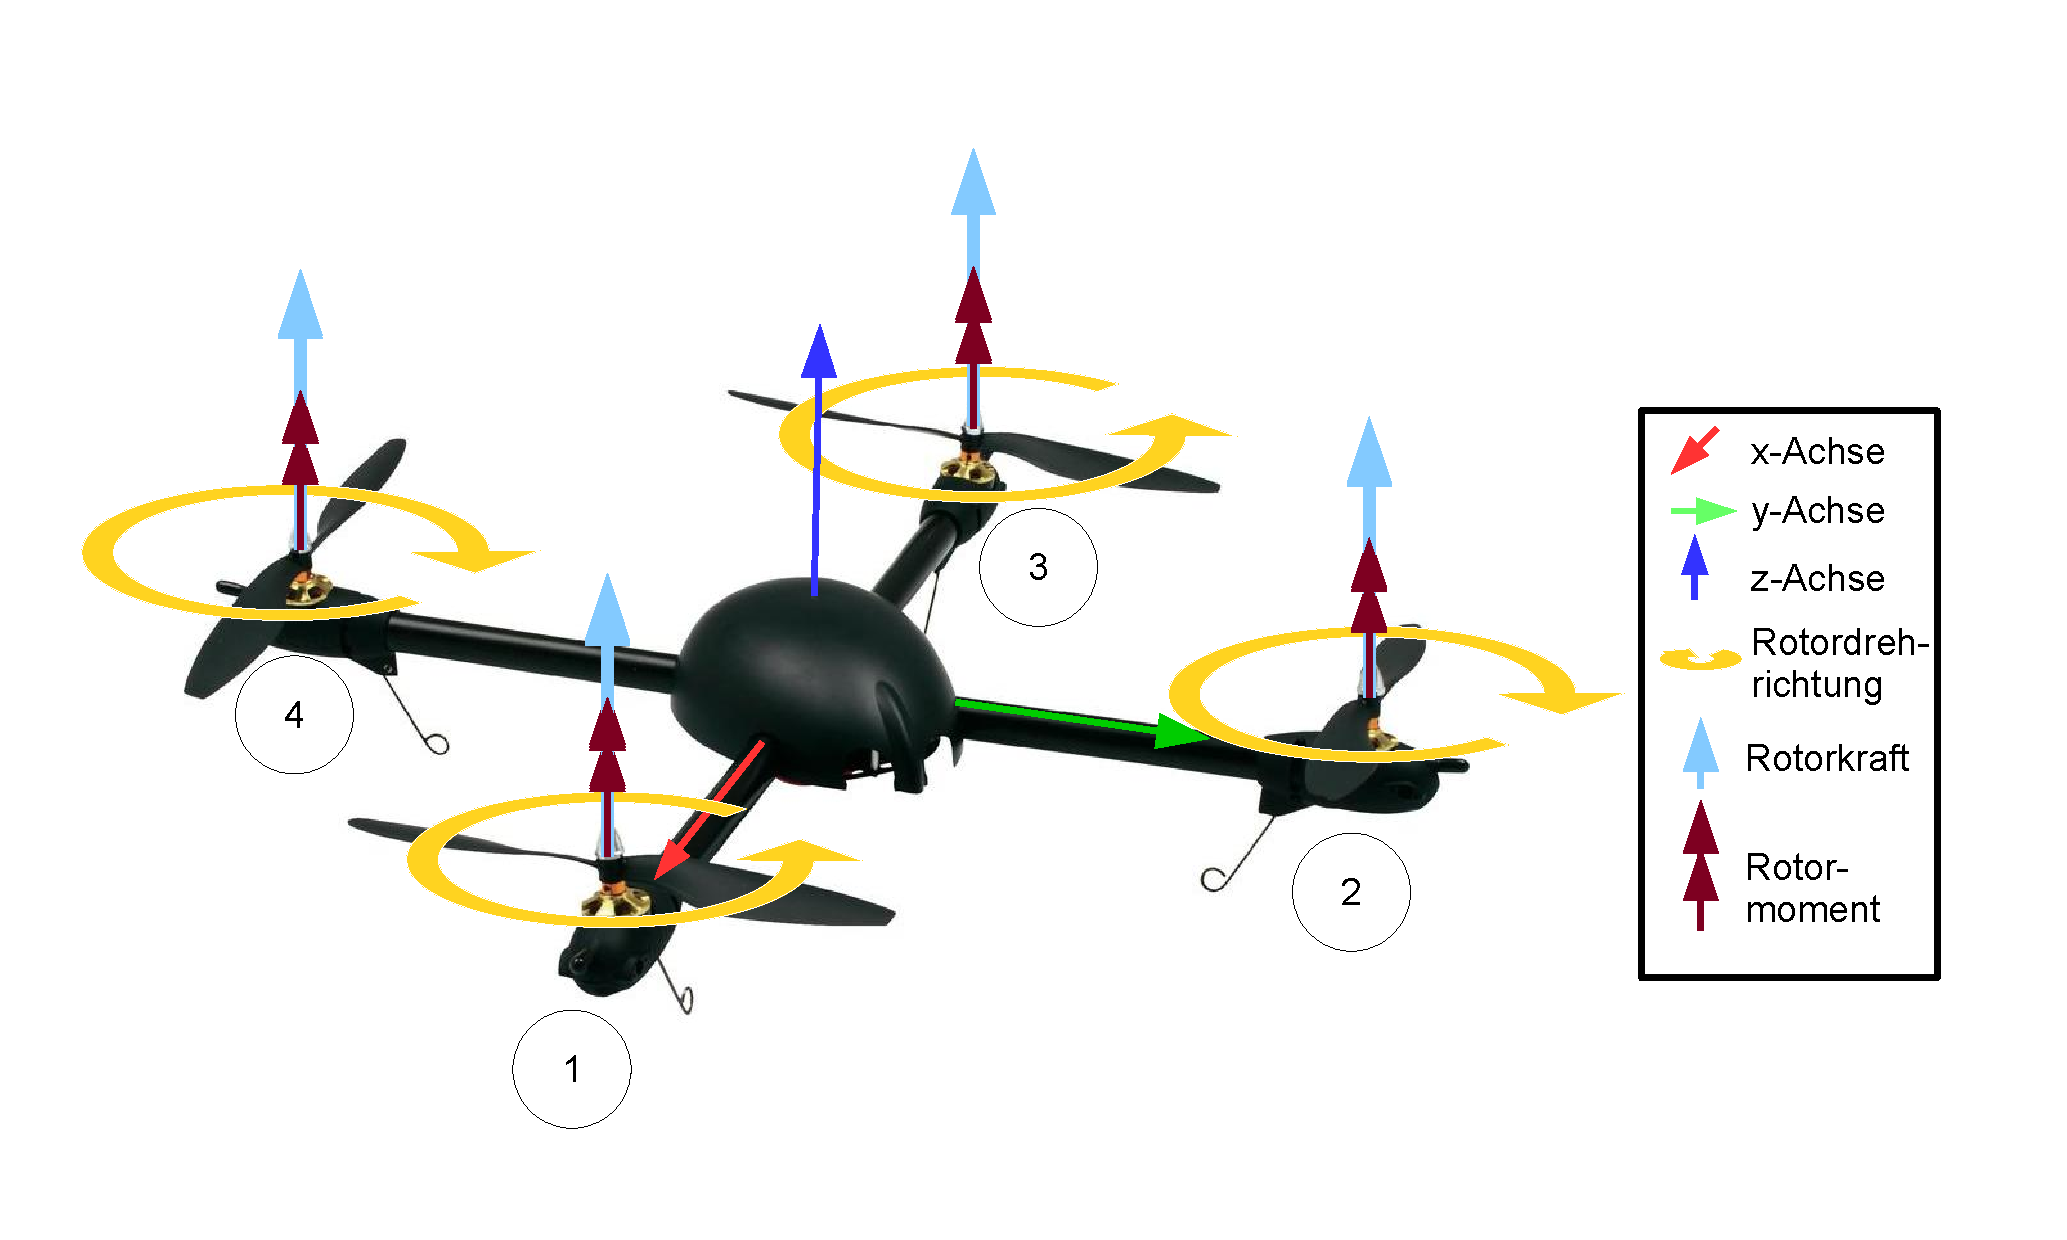
\includegraphics[width = 0.9\textwidth]{images/funktionsweise_quadrocopter}
	\caption[Momente und Kr�fte an einem Quadrocopter]{Momente und Kr�fte an einem Quadrocopter}
	\label{fig:funktionsprinzip}
\end{figure}

\begin{equation}
S^b = \begin{bmatrix}
S^{b}_x\\
S^{b}_y\\
S^{b}_z\\
\end{bmatrix}
=
\begin{bmatrix}
0\\
0\\
F_1+F_2+F_3+F_4\\
\end{bmatrix}
\label{eq:Schubvektor}
\end{equation}

Damit der Qudrocopter eine Bewegung im Raum vollziehen kann, muss dieser Vektor aus der Vertikalen ausgelenkt werden. Dies wird durch eine �nderung der Lage realisiert. Reduziert man zum Beispiel die Drehzahl $n_1$ und erh�ht gleichzeitig die Drehzahl $n_3$ hat das resultierende Kr�fteungleichgewicht �ber die L�nge $ l $ der Quadrocopterarme ein positives Moment um die $y^b$-Achse zur Folge. Der Quadrocopter dreht sich um die $y^b$-Achse, der Pitch-Winkel �ndert sich. Der Quadrocopter erf�hrt in der horizontalen Ebene des Raums eine Beschleunigung. Das gleiche Prinzip gilt auch f�r den Roll-Winkel, sprich Rotation um die $x^b$-Achse. Hier ist allerdings der Drehzahlenunterschied zwischen $n_2$ und $n_4$ verantwortlich f�r die Rotation.

Eine �nderung der Orientierung um die Hochachse z, sprich �nderung des Yaw-Winkels, l�sst sich ebenfalls �ber Variation der Rotordrehzahlen hervorrufen. Dabei kommt der Effekt zum tragen, dass der Widerstand der umgebende Luft entgegen der Drehrichtung der Motoren eine Kraft auf die Rotorbl�tter einpr�gt. Je nach Drehrichtung der Rotoren wirkt damit ein Moment auf den Quadrocopter.
% Somit �ber die Rotoren Momente auf den Quadrocopter wirken.
Diese Momente, die an den Armen des Quadrocopters angreifen, lassen sich zur Vereinfachung in den Schwerpunkt verschieben. Damit bei gleicher Drehzahl aller Rotorbl�tter ein Momentengleichgewicht herrscht, drehen sich die Motoren eins und drei gegen, die Motoren zwei und vier mit dem Uhrzeigersinn. Um die gew�nschte Rotation zu erzielen, wird die Drehzahl $n_1$ und $n_3$ erh�ht und gleichzeitig  $n_2$ und $n_4$  reduziert. Das Ergebnis ist eine Rotation in positive Richtung.

Zusammenfassen lassen sich die f�r die Rotation um die Quadrocopter-Achsen verantwortlichen Momente $M^{b}_{x,y,z}$ in einem Vektor $M^b$ zusammenfassen.  

\begin{equation}
M^b = \begin{bmatrix}
M^{b}_x\\
M^{b}_y\\
M^{b}_z\\
\end{bmatrix}
=
\begin{bmatrix}
l(F_3-F_1)\\
l(F_2-F_4)\\
M_1-M_2+M_3-M_4\\
\end{bmatrix}
\end{equation}

Aufzukl�ren ist, warum mit einer Erh�hung der Drehzahl auch immer eine Reduzierung des Gegenparts verkn�pft ist. Die Begr�ndung lautet, dass der Schubvektor $S^b$ durch eine Rotation m�glichst wenig beeinflusst werden soll.%, um mit der Gesamtschubvorgabe ganz einfach bestimmt zu werden. 


\section{Aufbau der Hardware}
\label{sec:Hardwareaufbau}
Zum Einsatz kommt der AscTec Pelican der Firma \gls{asctec} \cite{hmpgasctec}. Dieser Quadrocopter ist eine spezielle Entwicklung f�r die Forschung. Seine Turmstruktur erm�glicht eine einfache Integration zus�tzlicher Sensoren und Nutzlasten. Durch die Flexibilit�t im Aufbau ist das Ziel dieses Teilkapitels, einen �berblick zur Position der einzelnen Komponenten zu geben. Begleitend zum Text sind diese in Abbildung \ref{fig:hardwareaufbau} dargestellt.\\

	\begin{figure}
		\centering
		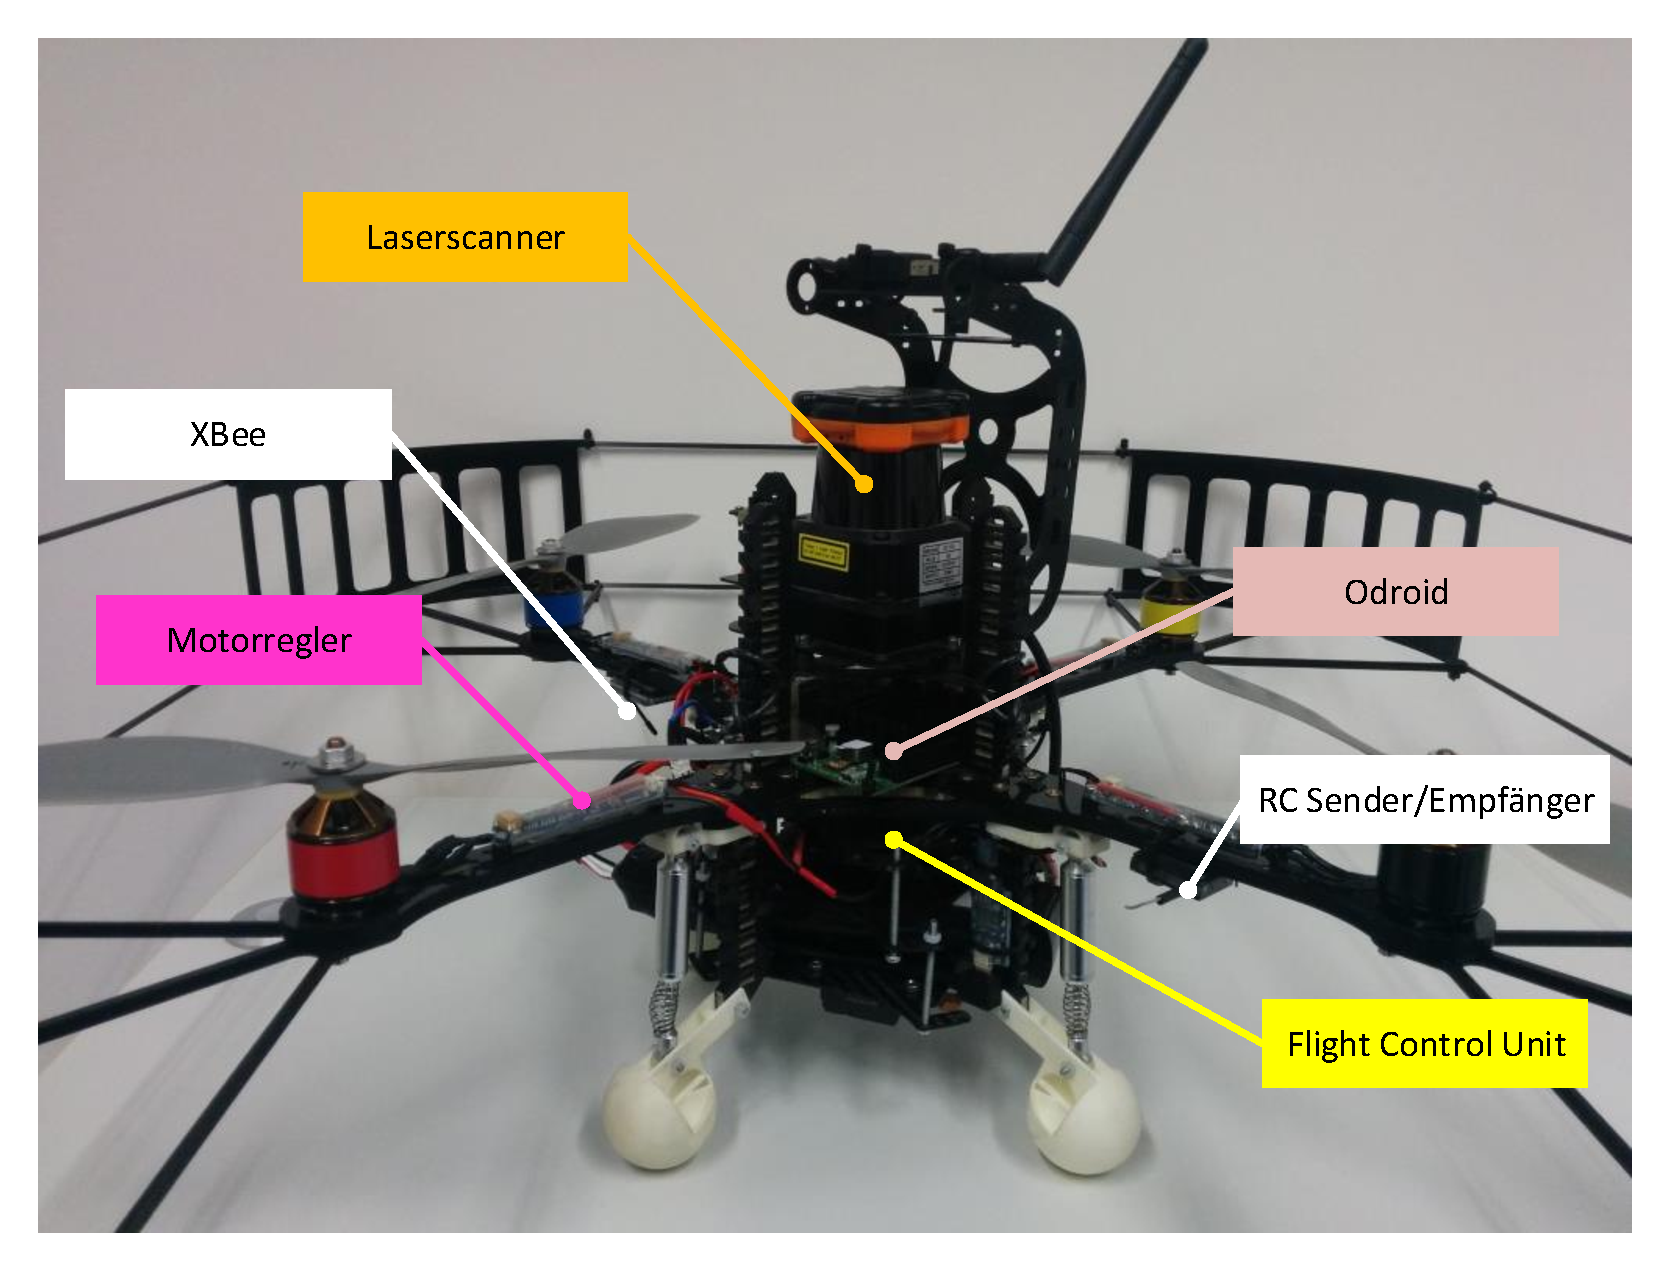
\includegraphics[width = 0.75\textwidth]{images/Hardwareaufbau}
		\caption[Hardwareaufbau des Quadrocopters]{Hardwareaufbau des Quadrocopters}
		\label{fig:hardwareaufbau}
	\end{figure}

F�r jeden der vier mit einem Propeller verbundenen Elektromotoren sind separate Motorcontroller zust�ndig. Diese sorgen daf�r, dass sich die von der \gls{fcu} angeforderten Drehzahlen einstellen.

Die \gls{fcu} ist die zentrale Steuer- und Regeleinheit des Quadrocopters. Sie besitzt zwei ARM7 Prozessoren, einen \gls{llp} und einen \gls{hlp}, zudem verschiedene Kommunikationsschnittstellen (vgl. Kapitel \ref{fig:Kommunikationsstruktur}). Zus�tzlich besitzt \gls{fcu} eine inertiale Messeinheit (engl. \gls{imu}). Diese Einheit wird zur Bewegungsdetektion sowie zur Bestimmung der Lage und Ausrichtung ben�tigt. Sie ist nicht zur Positionsbestimmung in einem ortsfesten Koordinatensystem geeignet. Bestandteile der \gls{imu} sind ein 3D-Beschleunigungssensor, drei Drehratensensoren (Gyros), ein Kompass sowie ein Drucksensor zur Ermittlung der Flugh�he anhand des Luftdrucks. Verbaut sind die Sensoren mit Ausnahme des Kompass direkt auf der Platine (Abbildung \ref{fig:fcuplatien}).

Da der Einsatzbereich im Indoorbereich liegt, ist der Drucksensor zur H�henbestimmung in geschlossenen R�umen nicht geeignet. Er liefert erst ab einer H�he von $ 5~m $ zuverl�ssige Werte. Daher wurde in einer vorangegangen Arbeit von Jan Kallwies \cite{JanKal13} die Hardware um ein Modul zur Messung der H�he im Indoorbereich erweitert. Auf diesem Modul befinden sich zwei Infrarotsensoren f�r den Nahbereich. Beide zusammen decken einen Bereich von $ 4~cm $ bis $ 142~cm $ ab. Erweitert wird der Messbereich durch einen Ultraschallsensor f�r Entfernungen von bis zu $ 5~m $. Aus diesen drei Sensordaten wird �ber einen Extended-Kalman-Filter die Flugh�he bestimmt. Eine genaue Beschreibung dieses Fusionsfilters kann in der Arbeit von Jan Kallwies \cite{JanKal13} nachgelesen werden. Da in der vorliegenden Arbeit die Navigation in der horizontale Ebene den Schwerpunkt darstellt, wird dieses Modul hier nicht weiter behandelt.

	\begin{figure}
		\centering
		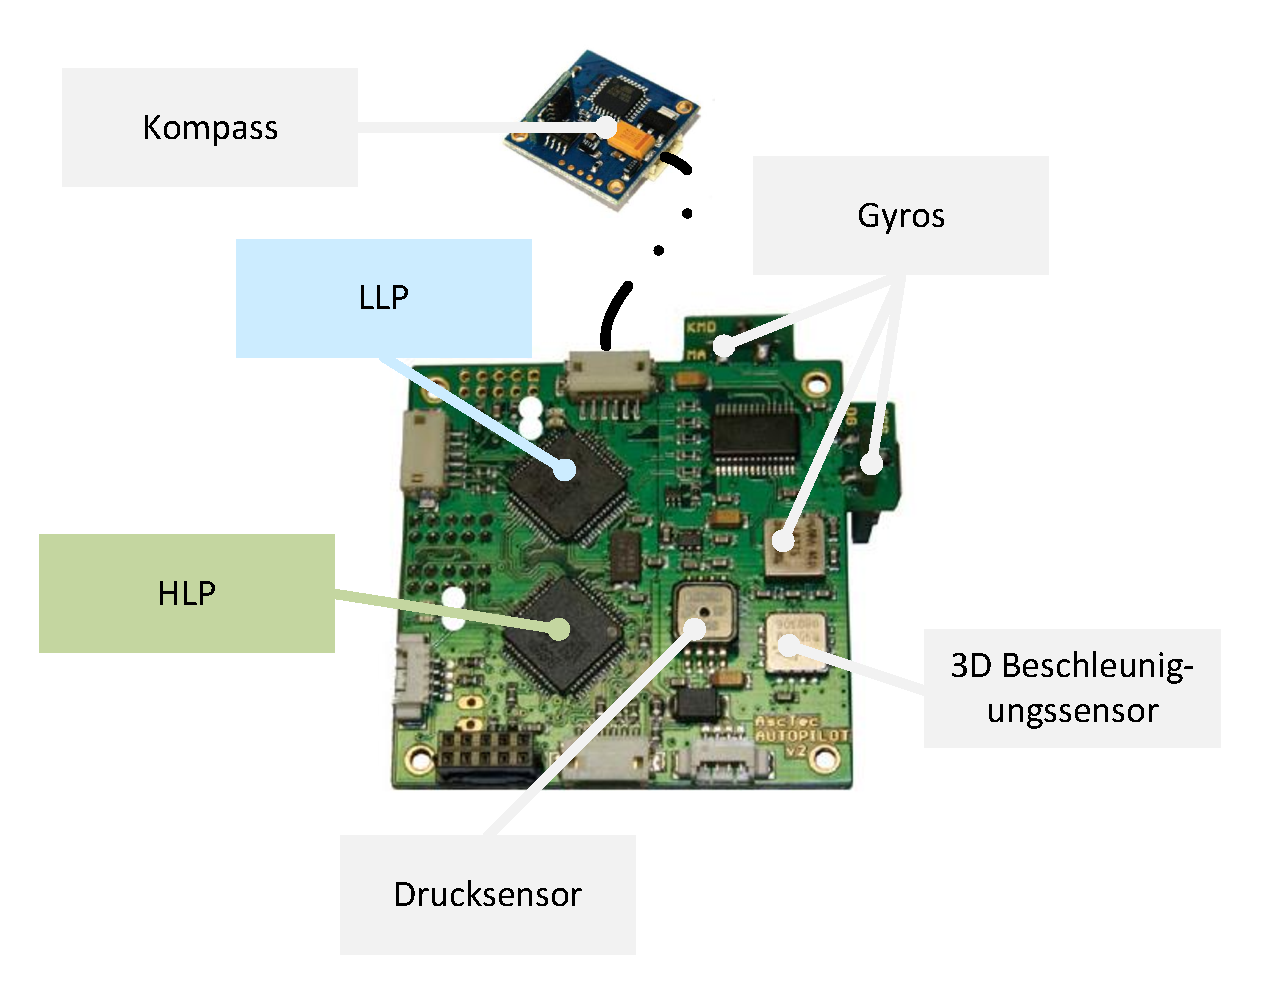
\includegraphics[width = 0.75\textwidth]{images/FCU_Platine}
		\caption[Platine der \gls{fcu}]{Platine der \gls{fcu}}
		\label{fig:fcuplatien}
	\end{figure}
	
Um in der Horizontalen die Navigation zu gew�hrleisten, muss die Position des Flugk�rpers in der xy-Ebene bekannt sein. Da dies, wie schon beschrieben, nicht mit der Inertialsenorik m�glich ist, wurde in die Turmstruktur der Laserscanner UTM-30LX der Firma Hokuyo (Datenblatt Anhang \ref{anh:datasheet}) integriert. Dieser Scanner hat eine maximale Reichweite von $ 30~m $ und ein Abtastbereich von $ 270^\circ $. Die Umlauffrequenz betr�gt dabei $ 40~Hz $, d.h. alle $ 25~ms $ steht ein neuer Scan zur Verf�gung.    

Damit zur Berechnung der Position sowie der Implementierung weiterer Algorithmen und Funktionen ausreichend Rechenleistung zur Verf�gung steht, befindet sich auf dem Quadrocopter ein zus�tzlicher Odroid-X Mikrocomputer mit einem Quad Core Prozessor mit $ 1.4~GHz $ und $ 1024~MB $ LP-DDR2 Arbeitsspeicher. Au�erdem besitzt diese Entwicklungsplattform sechs USB-Schnittstellen sowie einen $ 10/100~Mbps $ Ethernet-Anschluss.\\


%Nach dem �berblick �ber die im Quadrocopter verbaute Hardware und deren Komponenten, geht das folgende Kapitel \ref{sec:Kommunikationsarchitekur} auf die Implementierung der Intelligenz �ber Software ein.

%Nun sollte man einen �berblick �ber die im Quadrocopter verbauten Komponenten besitzen. Wie die Einheiten untereinander vernetzt sind, darauf wird im folgenden Kapitel \ref{sec:Kommunikationsarchitekur} eingegangen.

     
\section{Softwarearchitektur und Kommunikationsstruktur}
\label{sec:Kommunikationsarchitekur}

Nachdem im vorhergegangenen Kapitel \ref{sec:Hardwareaufbau} die verbaute Hardware vorgestellt wurde, geht es in diesem Abschnitt um die Softwarearchitektur (Abbildung \ref{fig:Kommunikationsstruktur}). Es wird aufgezeigt, welche Software bereits fest implementiert ist und wo adaptive Applikationen integriert werden k�nnen. Des Weiteren wird die Kommunikationsstruktur dargelegt, wie und �ber welche Protokolle die einzelnen Komponenten miteinander kommunizieren. \\
\begin{figure}
	\centering
	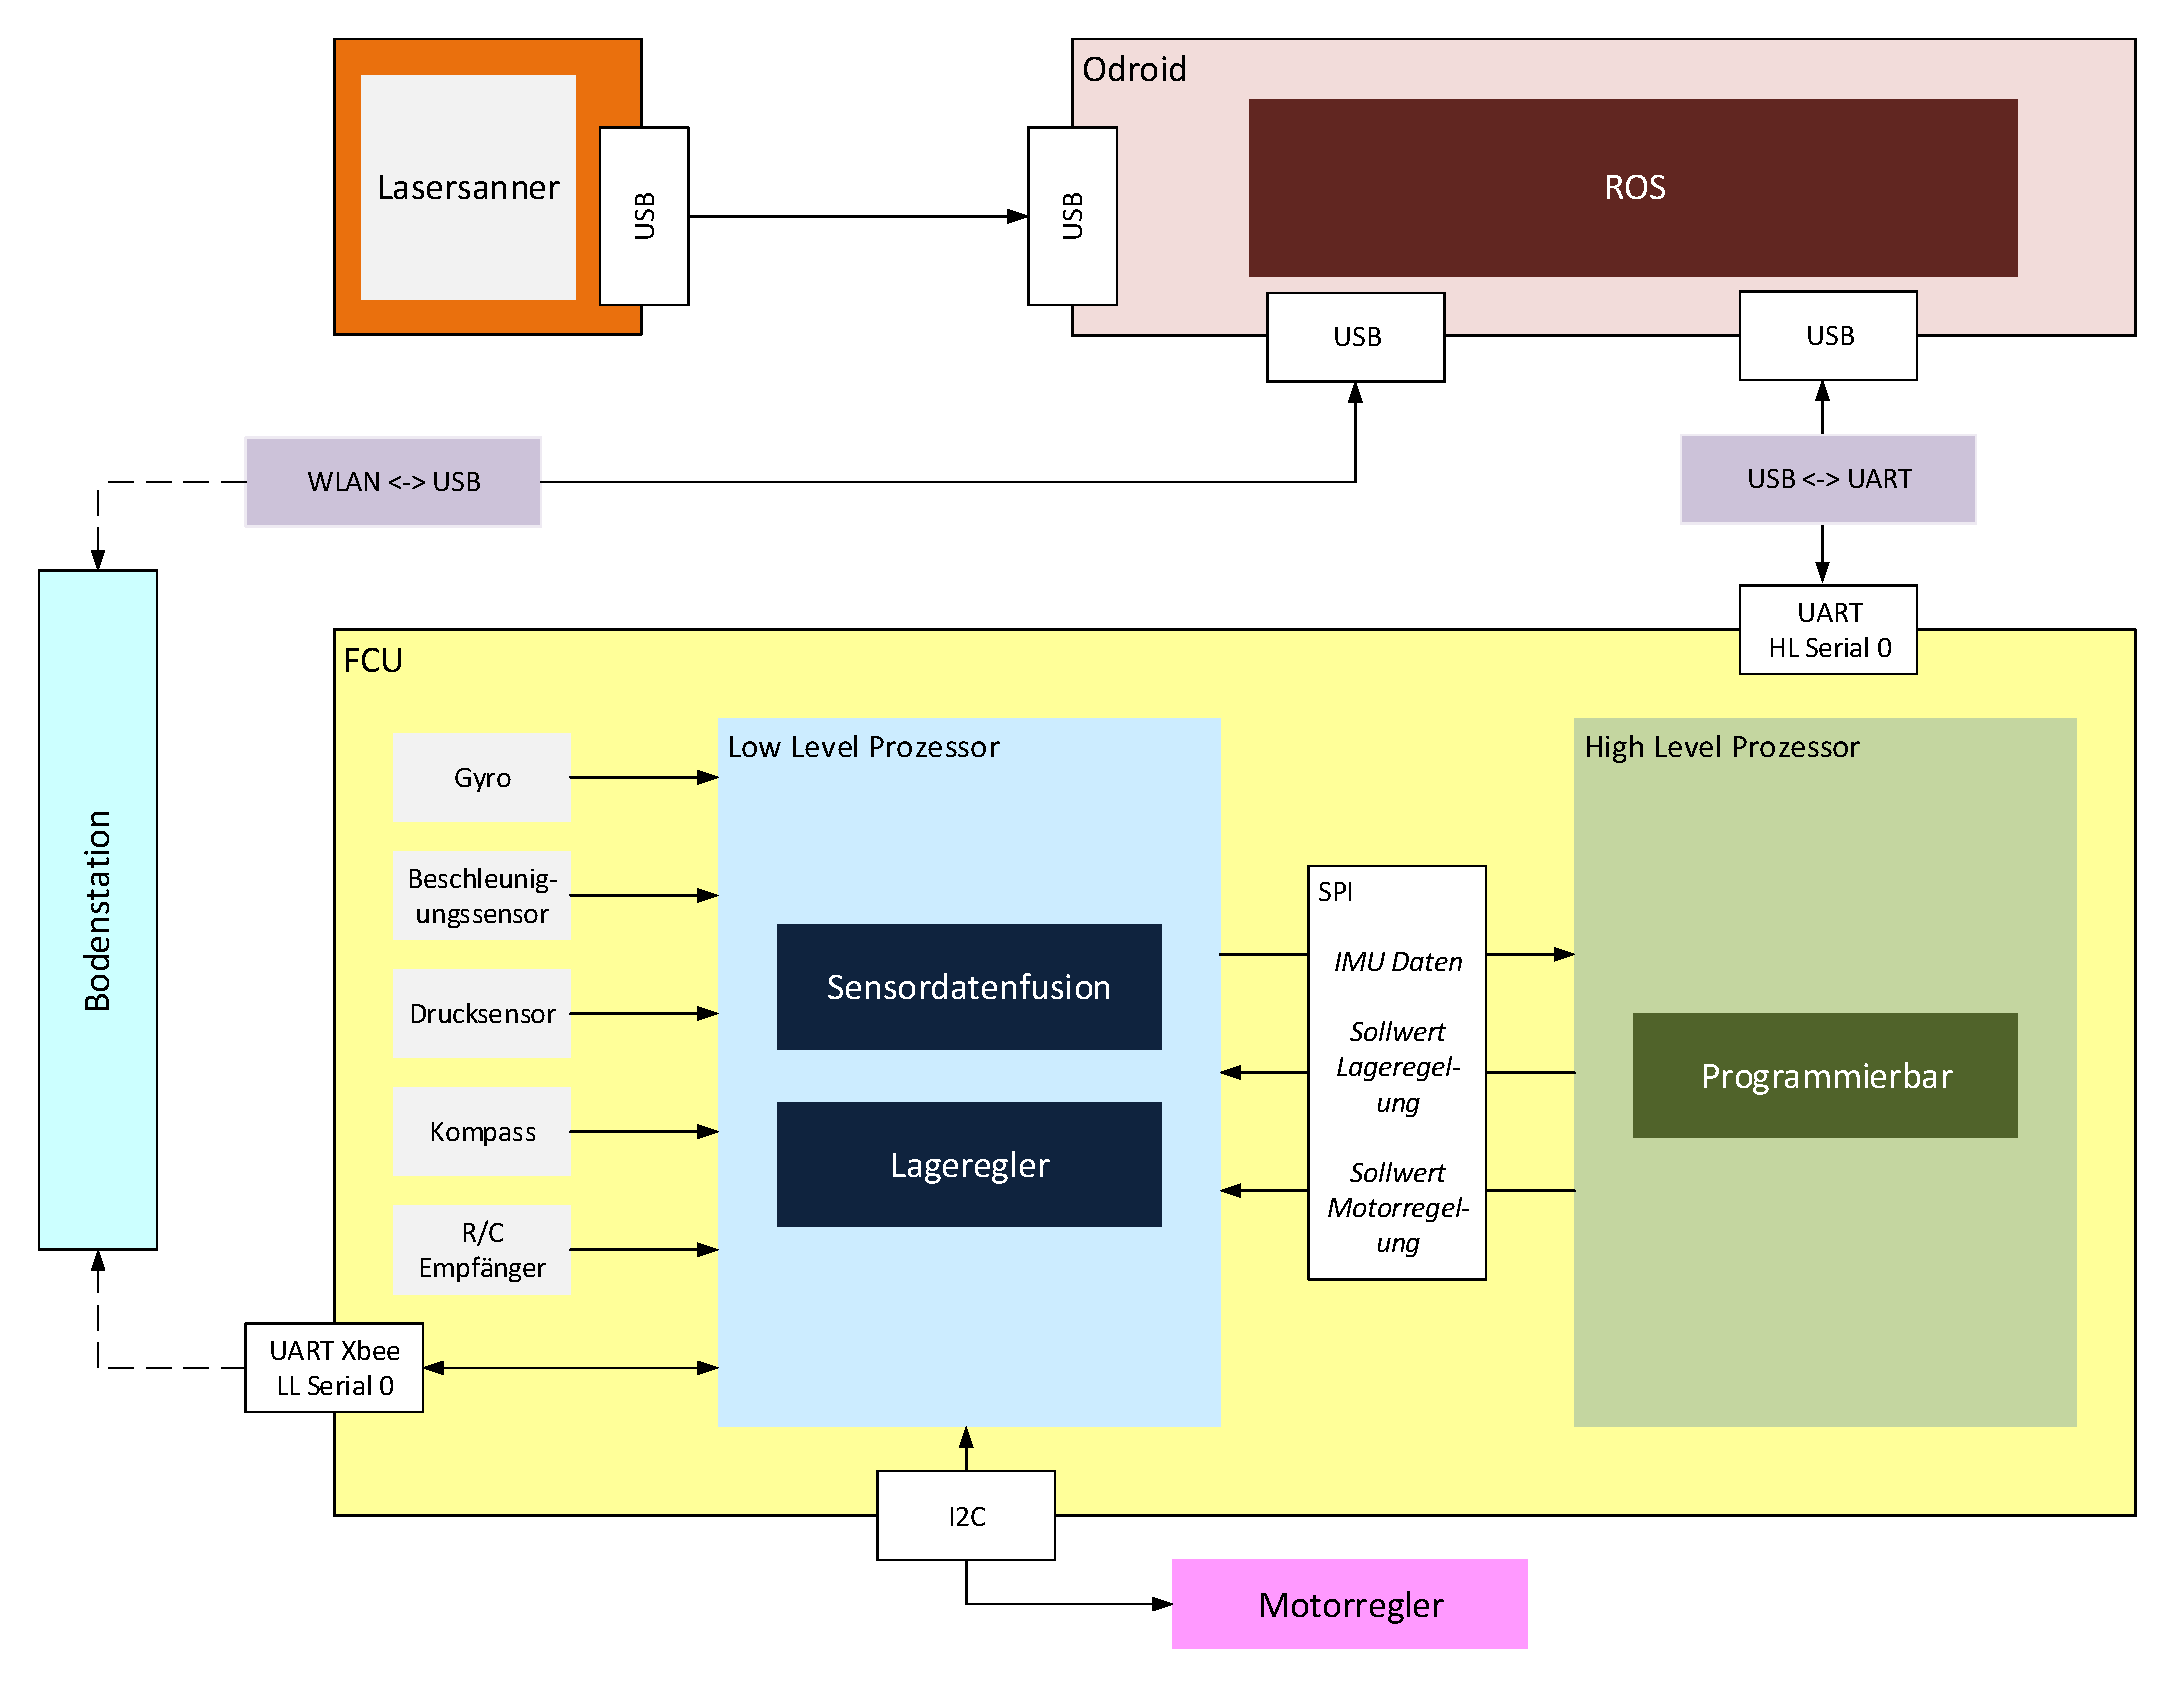
\includegraphics[width = \textwidth]{images/Kommunikationsarchitektur}
	\caption[Softwarearchitektur und Kommunikationsstruktur des Quadrocopters]{Softwarearchitektur und Kommunikationsstruktur des Quadrocopters}
	\label{fig:Kommunikationsstruktur}
\end{figure}
Beginnend mit den beiden Prozessoren 
%der \gls{llp} und \gls{hlp} 
der \gls{fcu}, deren Hauptschleifen der Software mit einer Frequenz von $ 1~kHz $ durchlaufen werden und die 
%mit der \gls{fcu}, deren beiden Prozessoren \gls{llp} und \gls{hlp} mit einer Frequenz von 1kHz getaktet werden und 
�ber einen \gls{spi} Bussystem verkn�pft sind, wird zun�chst der \gls{llp} betrachtet. Auf dem Low Level Prozessor befindet sich die Sensordatenfusion der \gls{imu}-Sensorik zur Lagebestimmung des Quadrocopters. Darauf basiert die Lageregelung, die das Flugverhalten stabilisiert. Hier�ber werden die geforderten Sollwinkel bzw. die Solllage eingestellt, die dem \gls{llp} �ber die Fernbedienung oder den \gls{hlp} �bergeben werden. Kombiniert mit der Schubvorgabe werden den Motorreglern die jeweiligen Solldrehzahlen der Rotoren �ber einen \gls{i2c}-Bus �bergeben. Diese Algorithmen sind fest eingepflegt und gew�hrleisten bei Experimentalfl�gen eine sichere R�ckfallebene. Mit dem \gls{llp} stellt \gls{asctec} dem Benutzer eine Art White-Box zur Verf�gung, d.h. die Integration ist bekannt, jedoch nicht deren Umsetzung. �berwachen l�sst sich der LLP �ber einen externen \gls{pc}, in Abbildung \ref{fig:Kommunikationsstruktur} als Bodenstation bezeichnet. Zur Kommunikation werden zwei XBee Funkmodule ben�tigt. Eines ist am \gls{uart} LL-Serial0 Port der \gls{fcu} angeschlossen, das andere am USB Port der Bodenstation. Mit der AutoPilot Software lassen sich unter anderem der Akkustand, die \gls{imu}-Daten sowie die Stellgr��en der Fernsteuerung betrachten. Au�erdem ist es m�glich, Parameter der Sensorfusion und der Lageregelung auszulesen und zu ver�ndern.


Mit dem \gls{hlp} stellt \gls{asctec} eine Entwicklungsumgebung zur Implementierung eigener Algorithmen auf der \gls{fcu} zur Verf�gung. Hier k�nnen erweiternde Programmteile integriert werden, die den Lageregler des \gls{llp} ansprechen oder die direkt den Motorcontroller �ber den \gls{llp} mit Solldrehzahlen speisen.

Die experimentelle Software auf dem \gls{hlp} kann �ber die Fernbedienung aktiviert und deaktiviert werden. Eine fehlerhafte Programmierung des \gls{hlp} kann kritische Flugman�ver hervorrufen. Damit diese nicht zum Absturz f�hren, kann �ber die Fernbedienung die Experimentalsoftware deaktiviert und das Flugsystem �ber die ausgereifte Lageregelung auf dem \gls{llp} stabilisiert werden (R�ckfallebene).

Wie schon in Kapitel \ref{sec:Hardwareaufbau} beschrieben, befindet sich auf dem Quadorcopter zur Erh�hung der Rechenleistung der Odroid-X. Anders als bei den auf der \gls{fcu} befindlichen Prozessoren, besitzt das Odroid-Bord ein Betriebssystem. Es handelt sich dabei um das opensource Betriebssystem Ubuntu 13.04. Dieses wurde ausgew�hlt, da es die Installation eines weiteren opensource Betriebssystems erm�glicht, dem \gls{ros}, einem Software Framework f�r Roboteranwendungen (Kapitel \ref{sec:ros}). Zum Einsatz kommt der Odroid-X bei der Implementierung der Positionsbestimmung (Kapitel \ref{chap:2Dpositionsbestimmung}). Verbunden ist es zum einen �ber einen USB-Port mit dem Laserscanner. Zum anderen mittels eines weiteren USB-Port �ber einen \gls{ftdi}-Konverter am HL-Serial0 Port des \gls{hlp} angeschlossen.
Von der Bodenstation kann �ber \gls{wlan} eine \gls{ssh}~-~Verbindung aufgebaut werden, die in Folge die Entwicklungsplattform bedient.

Nun ist bekannt, wie die einzelnen Komponenten untereinander vernetzt sind. Im weiteren Verlauf der Arbeit l�sst sich nachvollziehen, an welchen Stellen die Anwendungen implementiert werden und �ber welche Verbindungen sie miteinander kommunizieren. 


\chapter{Grundlagen}
\label{chap:grundlagen}
Das Kapitel Grundlagen behandelt die Themen, die in mehreren Abschnitten dieser Arbeit relevant sind. Dabei handelt es sich um das Robot Operation System, die verwendeten Koordinatensysteme und die Transformation zwischen ihnen.

\section{Das Robot Operation System \gls{ros}}
\label{sec:ros}
Ziel dieses Unterkapitel ist es das Opensource Betriebssystem \gls{ros} vorzustellen. Wie es aufgebaut ist und welche Vorz�ge es besitzt.\\

\gls{ros} stellt dem Softwareentwickler Bibliotheken und Werkzeuge zur Verf�gung, die Helfen Roboteranwendungen zu erstellen. Das auf einem \gls{ip}-basierende  modulare Kommunikationsframework erm�glicht die Verkn�pfung von Anwendungssoftware, Sensoren und Aktoren sogar unter mehreren Robotern. Die Grundlage daf�r ist die sogenannte Hardwareabstraktion. Dabei wird durch hardwarespezifische Module erreicht, das Komponenten unterschiedlicher Hersteller miteinander verbunden werden k�nnen. In unserem Fall Hokuyo Lasersanner und \gls{asctec} \gls{fcu}. Au�erdem erm�glicht es eine hardwareunabh�ngige Programmierung, die  in den Programmiersprachen C/C++ oder in Python erfolgen kann. Jede Hardwareabstraktion oder Anwendung wird als Node, bzw. Konten bezeichnet und l�uft als eigener Prozess.
\begin{figure}
	\centering
	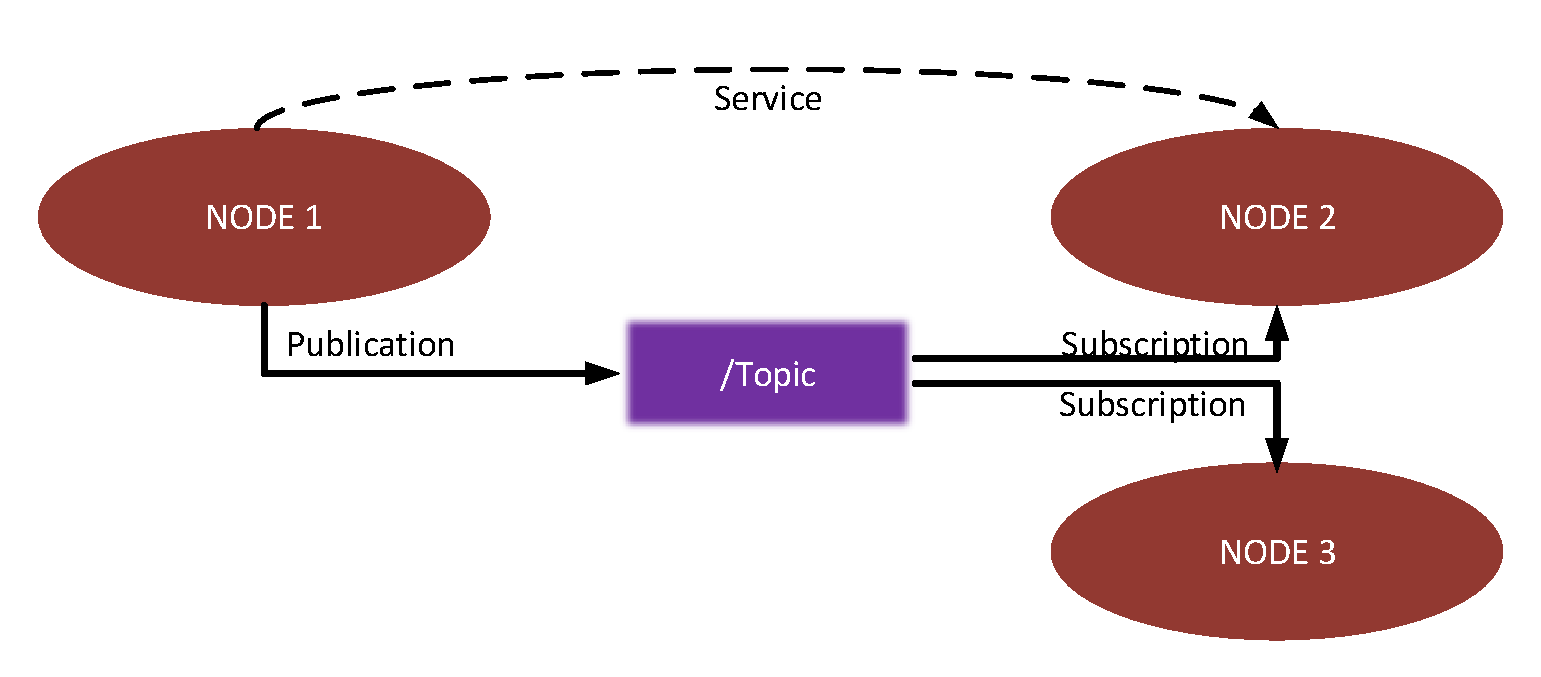
\includegraphics[width = 0.75\textwidth]{images/TopicUndService}
	\caption[Topic und Service]{Kommunikation von Nodes �ber Topics und Services}
	\label{fig:node_kommunikation}
\end{figure}


Der Austausch von Daten zwischen den Nodes erfolgt �ber so genannte Topics (Abbildung \ref{fig:node_kommunikation}]. Dabei werden von den Knoten Nachrichten (engl. Messages) in Topics gepostet und somit ver�ffentlicht (publication). Ben�tigt ein weiter Knoten den Inhalt dieses Topic kann er es abonnieren (subscription). Sobald die Nachricht im Knoten aktualisiert wurde, wird sie den abonnierenden Knoten �bertragen. Dabei sind Knoten nicht auf ein Topic beschr�nkt, es k�nnen beliebig viele Topics beschrieben oder empfangen werden. Alternative zu dieser Art der asynchronen Daten�bertragung, biete \gls{ros} die M�glichkeit einer Synchrone Kommunikation zwischen zwei Nodes �ber Services. Dabei wird auf einem Knoten ein Service gestartet. Dieser dient als Server und agiert nach dem Anfrage-Antwort-Prinzip. Schickt ein anderer Knoten eine Anfrage, wird ihm die geforderte Nachricht zu gesendet. 

Anzumerken ist, das durch das verwendete \gls{ip}-Protokoll keine deterministische Versendung der Nachrichten nicht gew�hrleistet ist, da es sein kann, das Nachrichten gleichen Types in Paketen zusammengefasst werden. Bei der Programmierung empfiehlt es sich daher auf Topics mit einem Zeitstempel (engl. timestamp) zur�ckzugreifen. Die Echtzeitf�higkeit des \gls{ros} ist durch allerdings nicht gef�hrdet. 

\begin{figure}
	\centering
	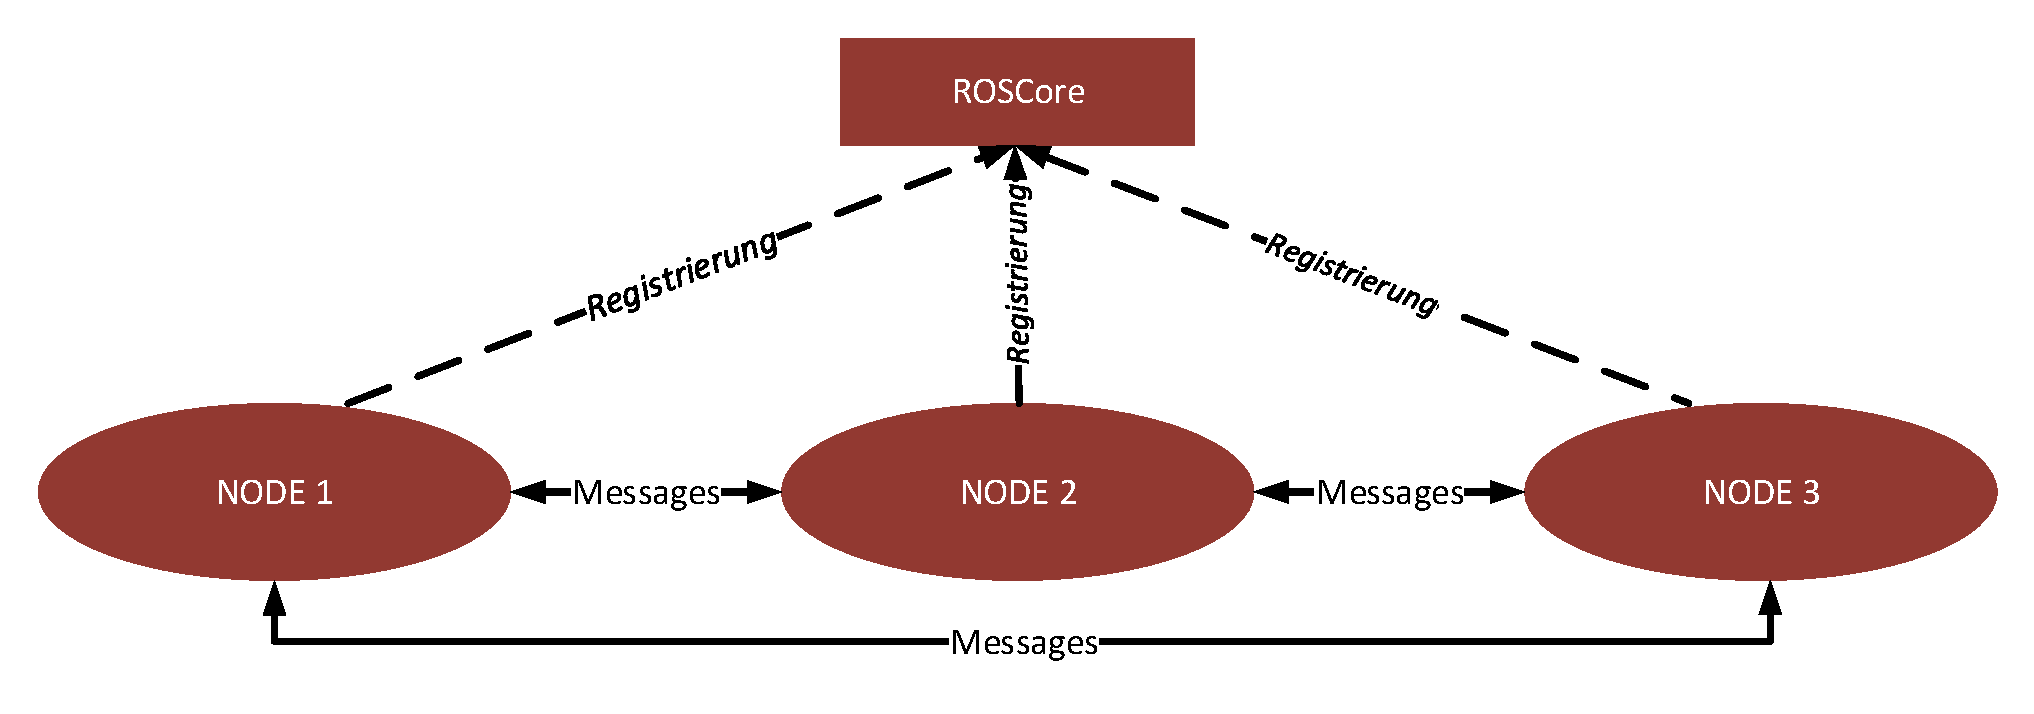
\includegraphics[width = \textwidth]{images/MasterAndNode}
	\caption[Registrierung der Knoten]{Registrierung der Knoten}
	\label{fig:node_master}
\end{figure}


Der wohl gr��te Vorteil von \gls{ros} ist die st�ndig wachsende Community. So stellen Forscher aus der ganze Welt ihre Algorithmen und Hardwareabstraktionen zur Verf�gung. Dadurch ist es m�glich bei der Erstellung einer Roboteranwendung auf Bausteine zur�ck zugreifen, die ohne diese Plattform selbst zu implementieren w�ren. Abgesehen davon stellt ROS eine Vielzahl von Hilfsmitteln wie zum Beispiel die Transferfunktion (/tf) bereit. Hier lassen sich Koordinatensysteme definieren. Die Transformation der Daten wird dann automatisch von \gls{ros} durchgef�hrt.

\section{Einf�hrung in die Koordinatensysteme und Koordinatentransformationen}
\label{sec:koordinatensysteme&transformationen}
Anhand von Koordinatensystemen und Transformationen l�sst sich die Lage von Punkten und  Objekten in einen Raum mathematisch beschreiben. Die Grundvoraussetzung zur Bestimmung der Position des Quadrocopters im 2D-Raum (siehe Kapitel HIER MUSS NOCH EINE REFERENZ HIN). Au�erdem erm�glicht die Einf�hrung von Koordinatensystemen die mathematisch/physikalische Beschreibung des Quadrocopters und stellt somit die Grundlage zur Modellbildung und Reglerentwurf (siehe Kapitel so und so).  

\subsection{Koordinatensysteme}
\label{subsec:koordinatensysteme}
�ber ein Koordinatensystem l�sst sich ein Vektor oder die Position eines Punktes bezogen auf den Koordinatenursprung in einer zweidimensionalen Ebene, bzw in einem dreidimensionalen Raum beschreiben. Ziel diese Teilabschnittes ist die Erl�uterung der in dieser Arbeit eingef�hrten Koordinatensysteme.\\

\begin{figure}
	
	\centering{
		\subfloat[ENU-Koordinatensystem]{
			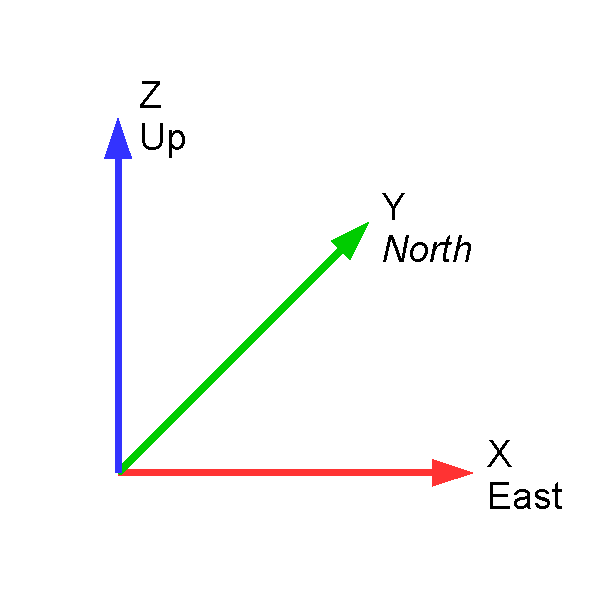
\includegraphics[width=0.3\textwidth]{images/ENU-koordinatensystem}
			\label{fig:enu}
		}
		\subfloat[NED-Koordimatemsystem]{
			\includegraphics[width=0.3\textwidth]{images/ned-koordinatensystem}
			\label{fig:ned}
		}
	}
	\caption[Kovention ]{test}
	\label{fig:konventionen}
	
\end{figure}

Zu Beginn werden nun zwei Konventionen bez�glich der Bezugssysteme vorgestellt. Nummer eins, die in Abbildung \ref{fig:enu} dargestellte \gls{enu} Konvention. Diese wird in vor allem bei der Landnavigation eingesetzt. Hier zeigt die z-Achse nach oben. Bei der zweiten Konvention, haupts�chlich in der Wasser-, Luft- und Raumfahrt eingesetzt, handelt es sich um das \gls{ned} Bezugssystem (Abbildung \ref{fig:ned}). Die z-Achse zeigt nach unten. Anzumerken ist, das in dieser Arbeit die Ausrichtung der x- und y -Achse nicht wie in Abbildung \ref{fig:konventionen} und auch der Namensgebung entsprechend den Himmelsrichtungen entspricht. Die Begriffe \gls{enu} und \gls{ned} dienen hier zur Beschreibung der Ausrichtung der Koordinatenachsen in Abh�ngigkeit der positiven z-Achse.

Bei der nun folgenden Einf�hrung der Koordinatensysteme (Abbildung \ref{fig:koordinatensysteme}) handelt es ausschlie�lich um kartesische, das hei�t orthogonale Koordinatensysteme, die nach der \gls{enu} Konvention ausgerichtet sind. Dies steht erstmal im Widerspruch mit dem Abschnitt zuvor, dort ist das \gls{ned} als Koordinatensystem f�r Flugk�rper eingef�hrt worden. Es ist allerdings so, dass die \gls{ros} Koordinatensysteme auf \gls{enu} basieren. Deshalb die Wahl von Bezugssystemen mit positiver z-Achse nach oben.

\begin{figure}
	\centering
	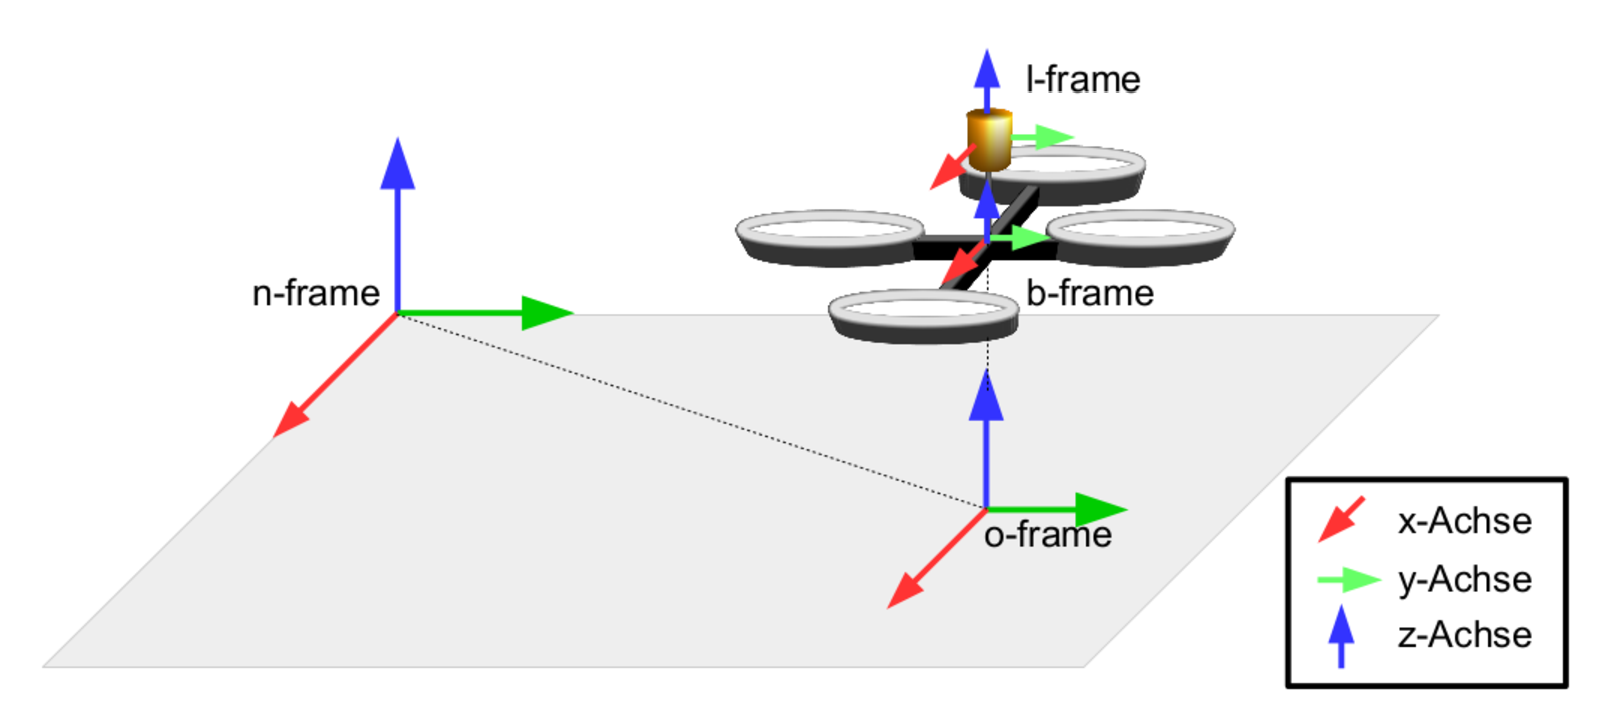
\includegraphics[width = \textwidth]{images/Koordinatensysteme}
	\caption[Koordinatensysteme]{In der Arbeit angewandte Koordinatensysteme }
	\label{fig:koordinatensysteme}
\end{figure}

Wie aus Abbildung \ref{fig:koordinatensysteme} zu entnehmen sind vier xyz-Koordinatensysteme definiert. 

\begin{itemize}
	\item \textbf{n-frame(Lokaler Navigationsframe):} Ortsfestes Koordinatensystem zur Beschreibung der Position im Raum. Da es in dieser Arbeit um die horizontale Positionsregelung geht, ist hier ausschlie�lich die xy-Ebene von Interesse. Der Ursprung des Koordinatensystem wird bei jedem Systemstart neu initialisiert. Zu beachten ist dies beim vollautonomen Flug in R�umen, dabei beziehen sich die Sollpositionen nicht auf ein Raumkoordinatensystem mit festem Ursprung, sondern auf den beim Systemstart initialsierten Bezugspunkt. Keinen Einfluss hat diese Tatsache auf die Geschwindigkeitsregelung per Fernsteuerung, da hier die relative Bewegung von Interesse ist.
	
	Es sei darauf hingewiesen, dass die Verwendung eines xyz Navigationsframes die Kr�mmung der Erdoberfl�che vernachl�ssigt. Diese ist legitim, da die Drohne in Geb�uden zum Einsatz kommt. M�chte man jedoch Weltweit navigieren, ben�tigt man ein  
	rotationsellipsische Koordinatensysteme[THIELECKE LITVERWEIS]

	\item \textbf{b-frame(Bodyframe):} Dieses Koordinatensystem ist fest mit dem Rahmen des Quadrocopters verbunden. Man spricht dabei von einen k�rperfesten Koordinatensystem. Dabei befindet sich der Ursprung des Systems im Schwerpunkt, die x-Achse zeigt in die als Vorne definierte Richtung. Die y- und z-Achse sind abh�ngig davon nach der \gls{enu} Konvention angeordnet. Informationen die sich auf dieses Referenzsystem beziehen sind unter anderen die \gls{imu}-Daten. Au�erdem l�sst sich mit diesem System die Lage des Quadrocoters im n-frame �ber die Position des Nullpunkts und Drehwinkel beschreiben. 
	 	
	\item \textbf{l-frame(laserframe):} Ebenfalls ein k�rperfestes Koordinatensystem. In die dem Entfernungsmessungen des Lasers aufgetragen werden. Der Bezugspunkt liegt dabei in der Sendequelle des Lasers. Die Ausrichtung der Achsen entspricht der des b-frames, mit Ausnahme eines Offsets in z-Richtung.
	
	\item \textbf{o-frame(Orthogonalframe):} Hierbei handelt es sich um ein objektbezogenes Bezugssystem, dessen Orientierung um seine z-Achse und die Position des Ursprungs im n-frame abh�ngig von dem Orthogonal �ber der Ebene befindlichen b-frame ist. Dadurch wird der Quadrocopter in der zu Navigierenden xy-Ebene abgebildet.  
	
	 \end{itemize}
 
Da sich Messwerte wie zum Beispiel die \gls{imu}-Daten oder die Laserdaten auf unterschiedlichen Koordinatensysteme beziehen, ben�tigt man Koordinatentransformation(Kapitel \ref{subsec:koordinatentransformation}). Mit Hilfe derer lassen sich die Vektoren und Koordinaten in die verschiedenen Bezugssysteme �bertragen.

 
\subsection{Koordinatentransformationen}
\label{subsec:koordinatentransformation}
Damit Daten eines Referenzsystem in einen anderes Transformiert werden k�nnen, muss deren Orientierung zueinander beschreibbar sein. Nach  [Buchholz Flugregelung] ist dies �ber die Rotationswinkel $\phi$ (Rollwinkel/engl. roll), Rotation um die x-Achse sowie der Winkel $\theta$ (Nickwinkel/engl. pitch) und $\psi$ (Gierwinkel/engl. yaw) f�r die y- und z-Achse m�glich. Die Reihenfolge um die die Achsen gedreht werden, ist dabei nicht beliebig. Sie ist in verschiedenen Konventionen festgelegt. In dieser Arbeit wird die in der Luftfahrt- und Fahrzeugtechnik gebr�uchliche z,y',x''- Konvention (Abbildung \ref{fig:zyx_konvention}) angewendet.   

\begin{figure}
	\centering
	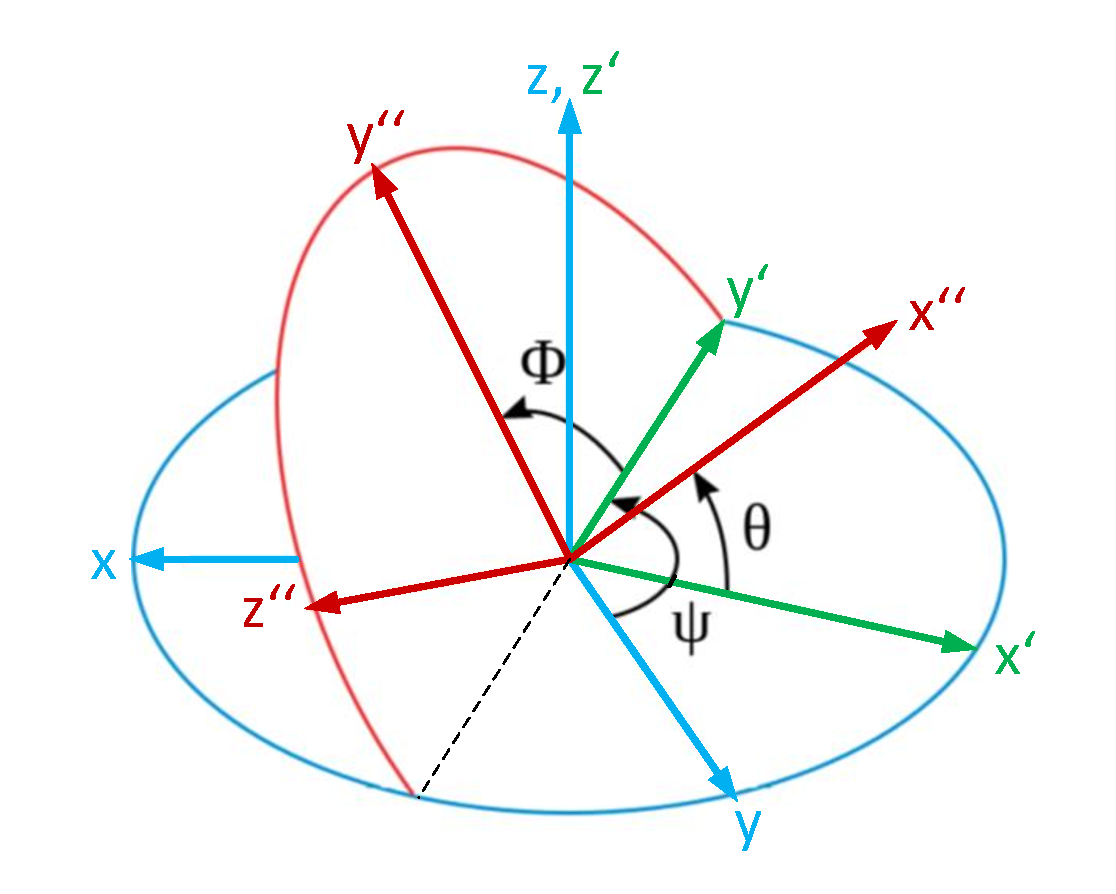
\includegraphics[width = .75\textwidth]{images/zyx_konvention}
	\caption[z,y',x''-Konvention]{z,y',x''-Konvention}
	\label{fig:zyx_konvention}
\end{figure}

Das Koordinatensystem wird zu beginn um den Winkel $\psi$, d.h. um die z-Achse gedreht. Daraus ergibt sich das in Abbildung \ref{fig:zyx_konvention} gr�n eingezeichnet Koordinatensystem. Dieses rotiert man anschlie�end um die Achse y', sprich den Winkel $\theta$. Zuletzt erfolgt eine Drehung mit dem Winkel $\phi$ um die x''-Achse. Das Ergebnis ist das rote x'',y'',z''-Koordinatensystem. Es sein nochmal darauf hinzuweisen, das die Reihenfolge der Winkel einzuhalten ist, da sonst die beschriebene von der tats�chlichen Lage abweicht. Ein veranschaulichendes Beispiel worin unterschiedliche Abfolgen bei der Rotation f�hren ist in der Literatur [Literaturverzeichnis] von Herr Thielecke zu finden.  

Nach Luftfahrtkonvention l�sst sich eine Transformationsmatrix $M$ aufstellen, mit der Vektoren und Koordinaten vom xyz-Koordinatensystem (Bsp.: n-frame) in das x''y''z''-Koordinatensystem (Bsp.: b-frame) �berf�hren lassen. Daf�r ben�tigt man zun�chst die drei Transformationsmatrizen, die jeweils eine Rotation um eine Koordinatenachse beschreiben[Literaturverzeichnis]. Diese sind wie folgt definiert:

\begin{itemize}
	\item Drehung um die z-Achse mit dem Winkel $\psi$
	\begin{equation}
		M_z = \begin{bmatrix}
		\cos\psi 	& -\sin\psi	& 0\\
		\sin\psi	& \cos\psi	& 0\\
		0			& 0 		& 1\\
		\end{bmatrix}
		\label{eq:Mz}
	\end{equation}
	\item Drehung um die y-Achse mit dem Winkel $\theta$
	\begin{equation}
	M_y = \begin{bmatrix}
	\cos\theta  & 0	& \sin\theta\\
	0			& 1	& 0\\
	-\sin\theta	& 0 & \cos\theta\\
	\end{bmatrix}
	\end{equation}
	\item Drehung um die x-Achse mit dem Winkel $\phi$
	\begin{equation}
	M_x = \begin{bmatrix}
	1	& 0			& 0\\
	0	& \cos\phi	& -\sin\phi\\
	0	& \sin\phi 	& \cos\phi\\
	\end{bmatrix}
	\end{equation}
\end{itemize}

Aus diesen Rotationsmatrizen l�sst sich �ber Matrizenmultiplikation eine Gesamttransformationsmatrix aufstellen. Die Reihenfolge der Multiplikation entspricht der in der Konvention festgelegten Drehfolge, von rechts nach links gelesen. Somit er gibt sich:

	\begin{equation}
	\begin{split}
	M_{bn} &	= M_x \cdot M_y \cdot M_z \\
	&= \begin{bmatrix}
	\cos\theta\cos\psi	& \cos\theta\sin\psi	& -sin\theta\\
	\sin\phi\sin\theta\cos\psi-\cos\phi\sin\psi	& \sin\phi\sin\theta\sin\psi+\cos\phi\cos\psi	& \sin\phi\cos\theta\\
	\cos\phi\sin\theta\cos\psi+\sin\phi\sin\psi	& \cos\phi\sin\theta\sin\psi-\sin\phi\cos\psi 	& \cos\phi\cos\theta\\
	\end{bmatrix}
	\end{split}
	\end{equation}
FORMEL �BERPR�FEN DA FEHLER IN ROATIONSMATRIZEN GEFUNDEN. DIESE SIND BEREITS BEHOBEN. NERNEUT �BERPR�FEN. WAR VORHER WAHRSCHEINLICH DOCH RICHTIG IN Gleichung POSE BESTIMMUNG HANDELT ES SICH IM EINE INVERSER ALSO TRANSFORMIERTE FORM VON MZ!!!!!!!!! Mz My Mx WAHRSCHEINLICH FALSCH SO WIE SIE DA STEHEN.
Mit Hilfe dieser Transformationmatrix l�sst sich jetzt ein Vektor zum Beispiel aus dem n-frame ins b-frame �bertragen.

\begin{equation}
\begin{bmatrix}
x^b\\
y^b\\
z^b\\	
\end{bmatrix} = M_{bn} \cdot 
\begin{bmatrix}
x^n\\
y^n\\
z^n\\	
\end{bmatrix}
\label{eq:inverse_transM} 
\end{equation}

Handelt es sich bei um eine Koordinate, ist zus�tzlich noch der Abstand der Koordinatenurspr�nge zu addieren. F�r die R�cktransformation muss die Gesamttransformationsmatrix transponiert werden. Daraus folgt,

   \begin{equation}
   \begin{bmatrix}
   x^n\\
   y^n\\
   z^n\\	
   \end{bmatrix} = M_{bn}^T \cdot 
   \begin{bmatrix}
   x^b\\
   y^b\\
   z^b\\	
   \end{bmatrix} = M_{nb} \cdot 
   \begin{bmatrix}
   x^b\\
   y^b\\
   z^b\\	
   \end{bmatrix}
   \label{eq:inverse_transM}
   \end{equation}

Nun lassen sich Vektoren in beide Richtungen in die verschiedenen Bezugssysteme �berf�hren. Nachteil der Methode mit Eulerwinkel ist, das diese auf Grund der trigonometrischen Funktionen nur f�r Winkel $\phi, \theta, \psi = \{x \in  \mathbb{R}| -\pi \le x \le \pi\}$ eindeutig durchf�hrbar ist. Wird dieser Bereich �berschritten, l�sst sich die Lage �ber Quaternionen beschreiben. Durch die Beschreibung der dreidimensionalen Orientierung in einem vierdimensionalen Raum lassen, ist die Lage auch f�r Rotationen um eine vielfaches von $2\pi$ eindeutig charakterisiert. Die genaue Definition findet sich in der  Literatur [THIELECKE] und [YOUTUBE]. Da die Definitionsbereich der Eulerwinkel f�r den in der Arbeit betrachteten Bereich ausreicht ist ausschlie�lich die Umrechnung der in Quaternion ($w_q$, $x_q$, $y_q$, $z_q$) angegebenen Orientierungsdaten der \gls{imu} in Eulerwinkel($\phi$, $\theta$, $\psi$). Zu beachten ist, das die nun folgende Umwandlung nur f�r die $z,y',x''$-Konvention G�ltigkeit besitzt. 
  
   \begin{equation}
	   \phi = \arctan(\frac{2(y_qz_q+w_qx_q)}{w_q^2-x_q^2-y_q^2+z_q^2})\\
	\end{equation}
   \begin{equation}
	  \theta =\arcsin(2(w_q y_q -x_q z_q))\\
   \end{equation}
   \begin{equation}
     \psi = \arctan(\frac{2(x_q y_q + w_q z_q)}{w_q^2+x_q^2-y_q^2-z_q^2})
   \end{equation}
 
 Mit dieser letzten Umrechnung sind alle Grundlagen f�r die Arbeit gelegt. So bilden die Koordinatensystem und Transformationen die Basis f�r die nachkommende Positionsbestimmung. 

\chapter[2D Positionsbestimmung]{Zweidimensionale Positionsbestimmung des Quadrocoters in xy-Ebene des Navigationsframes }
\label{chap:2Dpositionsbestimmung}
Wie schon in der Einleitung (Kapitel \ref{chap:Einleitung}) sowie der Aufgabenstellung Beschrieben, erfolgt die Positionsbestimmung �ber den auf dem Quadrocopter montierten Lasersanner. Man spricht hierbei von einem Onboard-Lokalisierungssystem. Die aufgenommen Entfernungen sind dabei im l-frame definiert. Die Rohdaten enthalten somit keine Information �ber die Position des Quadrocopters im Navigationskoordinatensystem, sondern jegentlich die Entfernung von umgebenden Objekten, bzw. W�nden. Anhand derer l�sst sich jedoch �ber die Methode des \glqq scanmatching\grqq  die Position in einer zweidimensionalen Ebene bestimmt werden (Kapitel \ref{sec:laser_scan_matching}). Da diese Ebene der xy-Ebene des n-frames entsprechen soll, m�ssen die Laserdaten zun�chst in das o-frame �berf�hrt werden (Kapitel \ref{sec:laser_ortho}). 


\begin{figure}
	\centering
	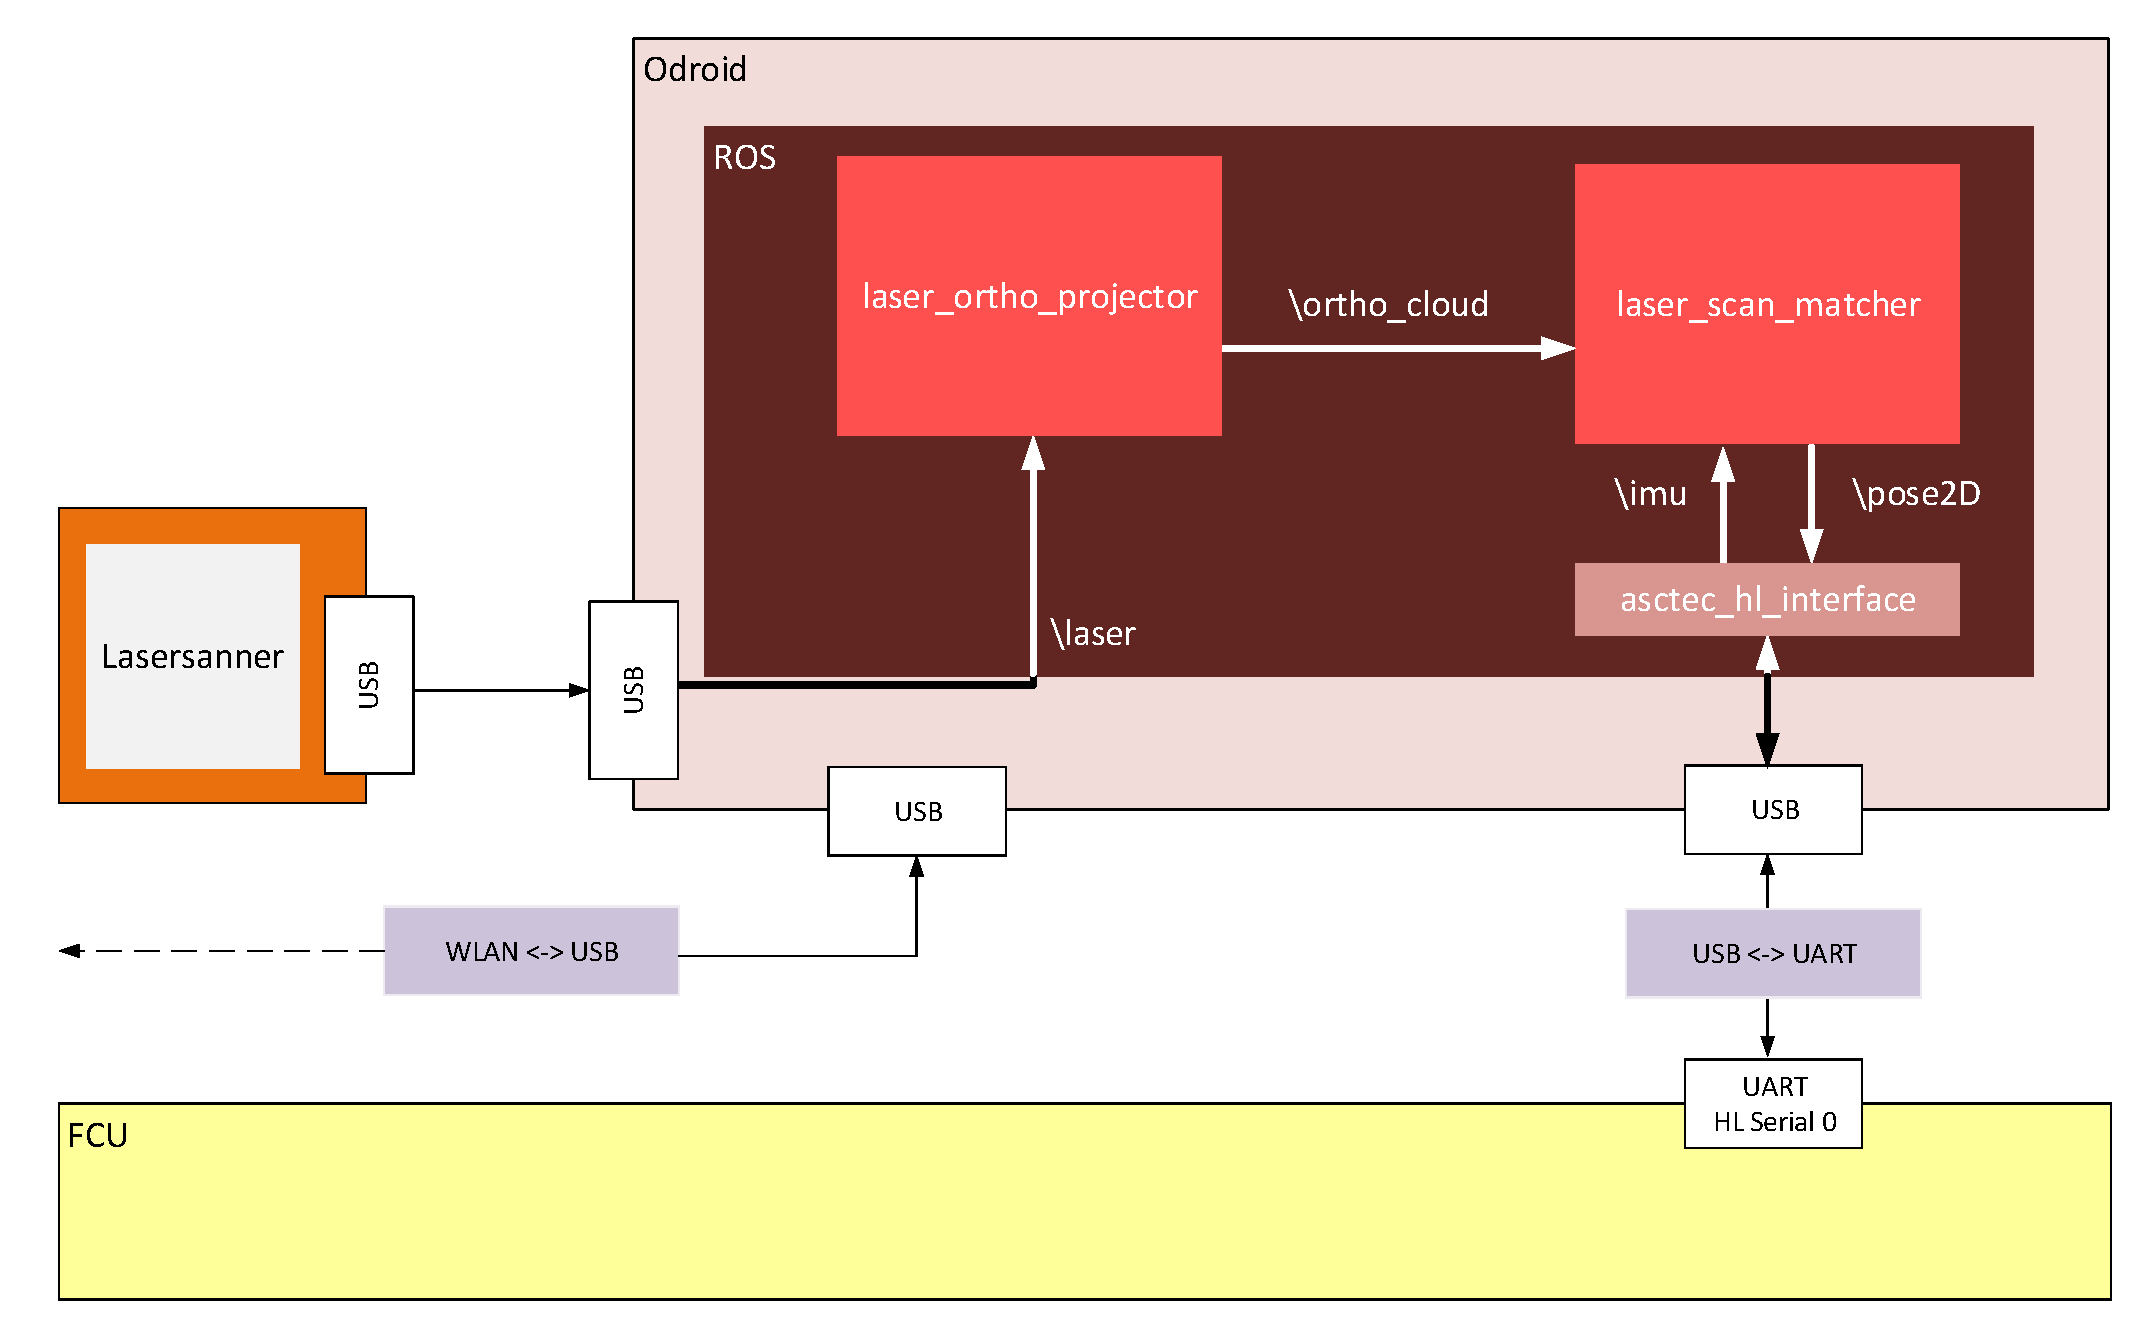
\includegraphics[width = .95\textwidth]{images/ros_ortho_scan_node}
	\caption[Verkn�pfung der Scantools]{Verkn�pfung des \glqq laser\_ortho\_projector \grqq - und des \glqq laser\_scan\_matcher\grqq -Knoten GRAFIK EVENTUELL �BERARBEITEN DA ASCTEC\_HL\_INTERFACE KNOTEN DER F�R DIE KOMMUNIKATION VERANTWORTLICH IST FEHLT} %
	\label{fig:verkn_scantools}
\end{figure}

Realisiert sind diese Vorg�nge in den von \gls{ros} zu Verf�gung gestellte scan\_tools.  Genauer gesagt handelt es sich dabei um dem \glqq laser\_ortho\_projector \grqq - und dem  \glqq laser\_scan\_matcher\grqq -Knoten (Abbildung \ref{fig:verkn_scantools}).Ziel der folgenden Kapitel ist es die Mathematik sowie die Funktionsweise die hinter diesen Algorithmen steht zu erl�utern. 	

ANMERKUNG ES FEHLT NOCH EIN LITERATURVERZEICHNIS!	



\section{Projektion der Laserdaten in das o-frame auf der xy-Ebene des n-frames (\glqq laser\_ortho\_projector\grqq) }
\label{sec:laser_ortho}
Bei der Laserprojektion werden die Laserdaten des l-frame orthogonal zur xy-Ebene des n-frames in die des o-frame transformiert. In allgemeiner Form ist dies in Abbildung \ref{fig:laser_proj_allg} dargestellt. Das o-frame definiert sp�ter in Kapitel \ref{sec:laser_scan_matching} die Position und Orientierung des Quadrocopters in der zweidimensionalen Ebene des n-frame. 
\begin{figure}
	
	\centering{
		\subfloat[Allgemeine Projektion der Laserdaten]{
			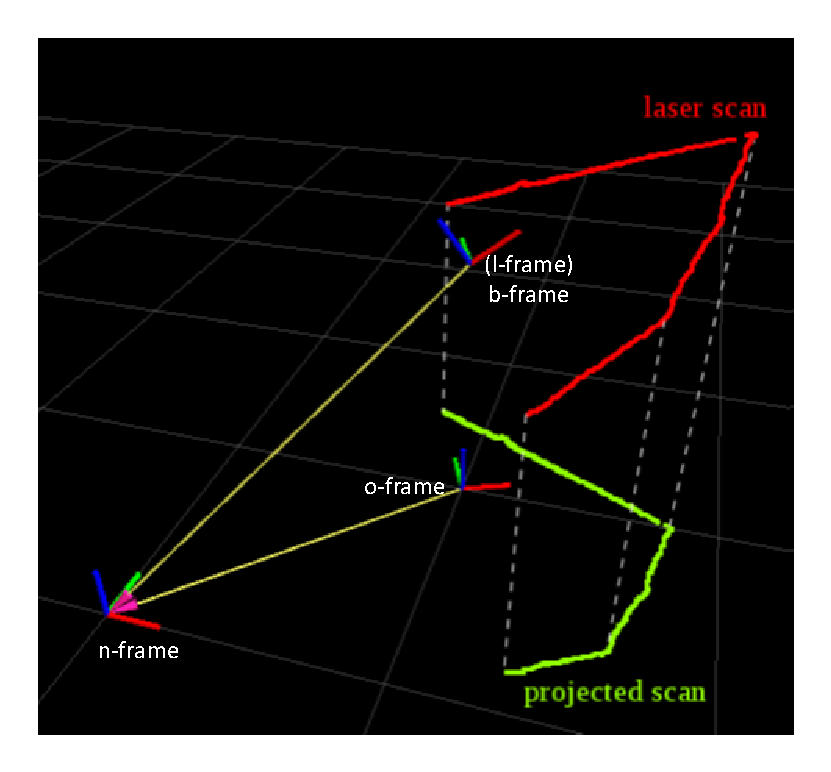
\includegraphics[width=0.5\textwidth]{images/laser_scan_project}
			\label{fig:laser_proj_allg}
		}
		\subfloat[Projektion eines Punkt $P_i$ in den o-frame]{
			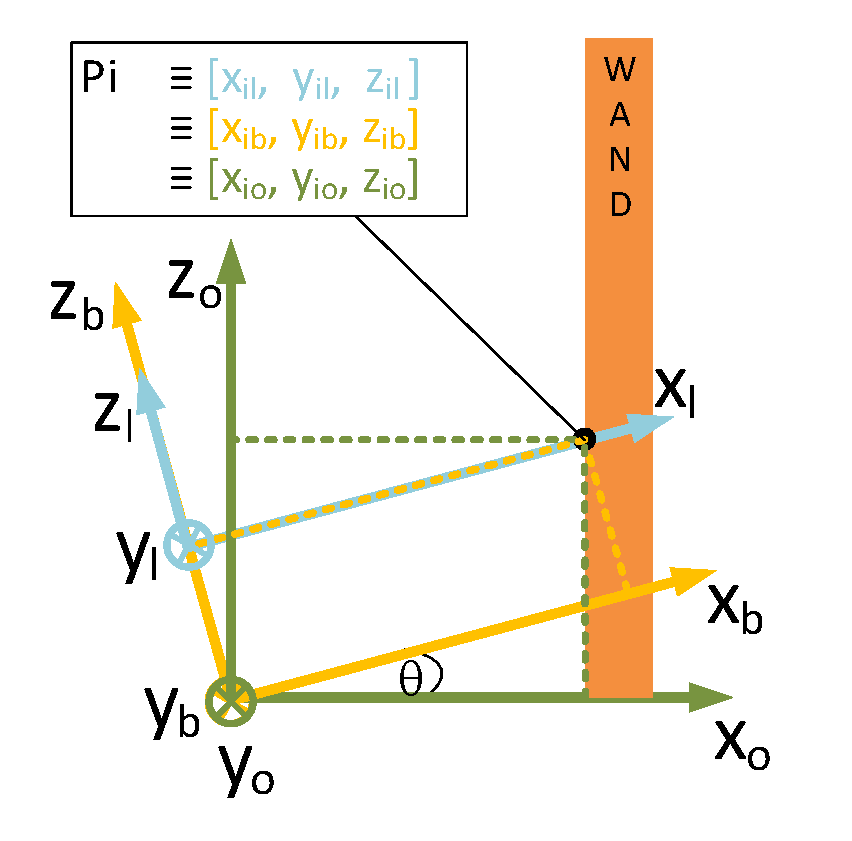
\includegraphics[width=0.5\textwidth]{images/laser_ortho_pro_zx_bsp}
			\label{fig:laser_proj_pi}
		}
	}	
	\caption[Laserprojektion]{Projektion der Laserdaten}
	\label{fig:laser_proj}
	
\end{figure}
M�glich ist die orthogonalen Projektion nur unter der Annahme, das es sich bei den erfassten Objekten um Gegenst�nde mit rechtwinkligen Eigenschaften handelt. Das bedeutet sie weisen unabh�ngig der H�he in der sie erfasst werden die gleich Formen auf. F�r geschlossen R�umen ist diese Annahme zutreffend, da es sich bei den Objekten haupts�chlich um senkrechte W�nde handelt. Durch Erf�llung dieser Voraussetzungen kann die Flugh�he des Quadrocopters vernachl�ssigt werden. Dies kann man aus Abbildung \ref{fig:laser_proj_pi} entnehmen. Eine Verschiebung des Koordinaten Ursprungs des b-frames auf der z-Achse des o-frames hat demzufolge keinen Einfluss auf die Projektion. Folglich kann f�r beide Koordinatensystem der identischen Ursprung angenommen werden. Unter Beachtung dieser Annahmen kann der Einfluss des Roll-($\phi$) und Nickwinkels ($\theta$) auf die Entfernungsmessung eliminiert werden. Die Winkelgr��en liefert die \gls{imu}. Der mathematische Ablauf der orthogonalen Transformation wird basierend auf Literatur \cite{Morris2010}  im Folgenden dargelegt.\\


Entfernungsdaten eines Laserumlaufs besteht aus mehreren diskreten Abtastungen (Abbildung~\ref{fig:l-frame}). �bergeben werden sie in Form von Entfernung $r_i$ in einem Array (Topic \textbackslash laser Abbildung \ref{fig:verkn_scantools}). Mittels der Schrittweite von $0.25^\circ$ l�sst sich anhand des Indizes $i$ f�r jeden Messpunkt einen Winkel $\gamma_i$ zuweisen. 
\begin{equation}
\gamma_i = 135^\circ - 0.25^\circ \cdot i
\end{equation}

\begin{figure}
	\centering
	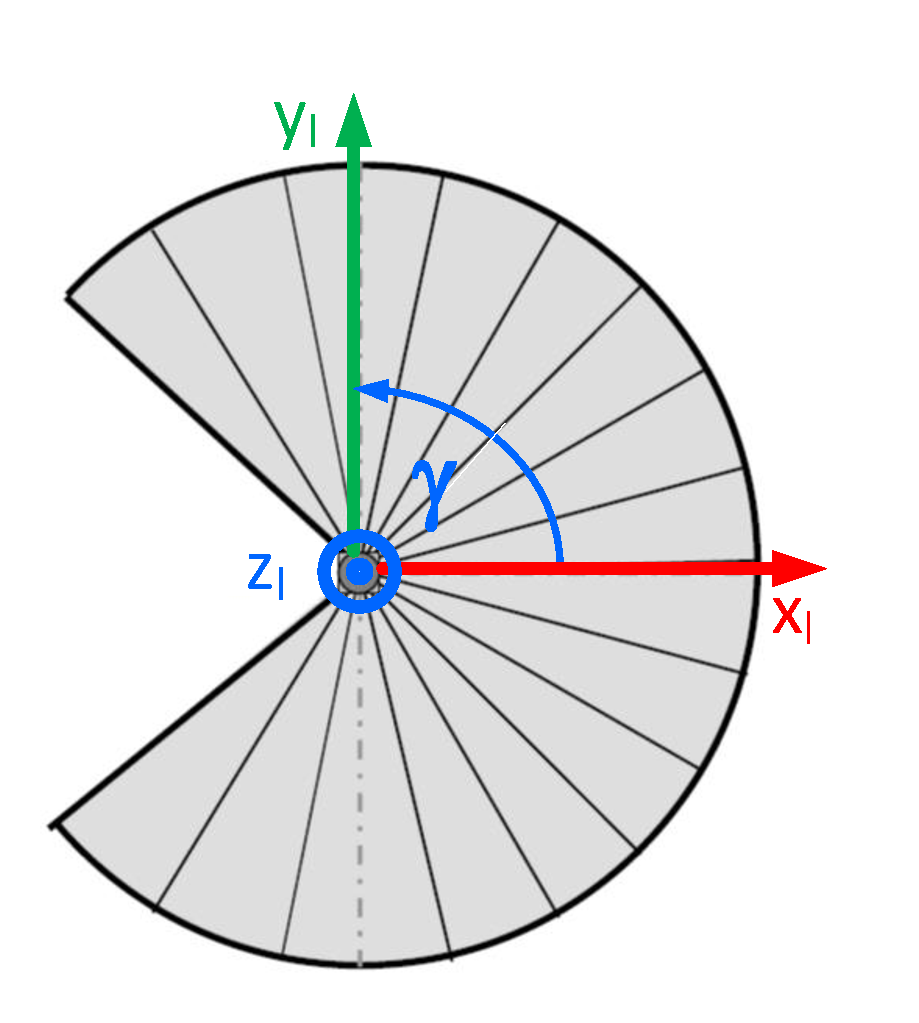
\includegraphics[width = .55\textwidth]{images/l_frame}
	\caption[l-frame]{Draufsicht l-frame} %
	\label{fig:l-frame}
\end{figure}

Die Entfernung eines Punktes $p_i$ ist somit �ber $\{r_i, \gamma_i\}$ definiert. Zur weiteren Verwendung ist es notwendig die Messungen im kartesischen Koordinatensystem des l-frame zu �bertragen.

  \begin{equation}
  p_i^l = 
  \begin{bmatrix}
  \cos(\gamma_i)\cdot r_i, & \sin(\gamma_i)\cdot r_i, & 0
  \end{bmatrix}^T
  \end{equation}
  
Da der Bezugspunkt des o-frames im Schwerpunkt des Quadrocoptes liegen soll, in dem auch der b-frame seinen Ursprung hat, ist es von n�ten die Laserdaten vom l-frame ins b-frame zu transformieren. Wie schon in Kapitel \ref{sec:koordinatensysteme&transformationen} erw�hnt handelt es sich dabei um eine konstante Transformation. Genauer gesagt um einen Offset von $10cm$ auf der $z^b$-Achse, da der Laser oberhalb des Quadrocopterschwerpunktes montiert ist.

\begin{equation}
p_i^b = 
\begin{bmatrix}
\cos(\gamma_i)\cdot r_i, & \sin(\gamma_i)\cdot r_i, & 0.1
\end{bmatrix}^T
\end{equation}

Nun da die Laserpunkte im b-frame definiert sind, kann die Transformation der Umgebungsdaten in die xy-Ebene des o-frames erfolgen. Angesichts der Tatsache, das die Winkel $\phi$ und $\theta$ als Verdrehung um die Achsen des o-frames definiert sind, ben�tigt man zur Umrechnung der Laserdaten die in Kapitel \ref{sec:koordinatensysteme&transformationen} eingef�hrte Gleichung \ref{eq:inverse_transM} zur inversen Koordinatentransformation. Dabei wird der Yaw-Winkel zu Null gesetzt. Grund hierf�r ist, das Ausrichtung der Flugrichtung in der zweidimensionalen Ebene mit der des b-frames �bereinstimmen sollen. Daraus ergibt sich f�r die Transformationsmatrix   

\begin{equation}
M_{no} = 
\begin{bmatrix}
\cos\theta\cdot r_i, 	& \sin\phi \sin\theta 	& \cos\phi \sin\theta\\
0 						& \cos\phi 				& -\sin\phi \\
-\sin\theta				& \sin\phi \cos\theta	& \cos\phi \cos\theta
\end{bmatrix}
\end{equation},

�ber die sich die Positionen der Laserpunkte $P_i^b$ im o-frame bestimmten lassen.  
\begin{equation}
p_i^o = M_{no} \cdot P_i^b
\end{equation}

Erneut kann unter der Annahme von rechtwinkligen Objekten die H�he des Punktes in $z^o$-Achse zu Null gesetzt werden. Somit sind die Punkte $p_i^l$ auf der xy-Ebene des o-frame folgenderma�en abgebildet.

\begin{equation}
p_i^o =  
\begin{bmatrix}
\cos\theta \cos(\gamma_i)\cdot r_i + \sin\phi \sin\theta \sin(\gamma_i)\cdot r_i + cos\phi sin\theta \cdot 0.1\\
\cos\phi\sin(\gamma_i)\cdot r_i - sin\phi \cdot  0.1\\
0
\end{bmatrix}
\end{equation}

Alle Punkte $p^o_i$ eines Umlaufs einen Scan $S$.
 
 \begin{equation}
 S^o = [p^o_i | i=1..1080]  
 \end{equation}
 
Diese Beschreibung $S$ der Laserscans im o-frame ist die Basis f�r die im anschlie�ende Kapitel \ref{sec:laser_scan_matching} behandelte Positionsbestimmung in der zweidimensionalen Ebene des n-frames. 


\section[Positonsbestimmung �ber Scanmatching]{Positionsbestimmung anhand der ins o-frame �berf�hrten Laserdaten �ber scanmatching}
\label{sec:laser_scan_matching}  
Aufbauend auf den im Kapitel \ref{sec:laser_ortho} vorgestellten Laser\_ortho\_projektor, ist es Aufgabe des Folgenden Teilkapitels zu erl�utern wie anhand eines Referenzscans $S_{ref}$ und einem weiteren Scan $S_{neu}$ die Position in der euklidischen xy-Ebene des n-frames bestimmt werden kann. Zur Anwendung kommt hier die Methode des Scanmatching. Dabei gilt die Annahme, das f�r jeden Scan $ S_{neu} $ und dessen dazugeh�rigen Position $ P_{neu} $ eine Rotation $ M^o_z $ um $ \psi^o $, inklusive Translation $ T $ existiert,  so dass die beiden Datenwolken $ S_{neu} $ und $ S_{ref} $ �bereinander liegen (Abbildung \ref{fig:prinzip_scanmatching}). Definiert ist $ S_{ref} $ dabei an der Stelle $ P_{ref} $.\\
\begin{figure}
	\centering{
		\subfloat[$S_{ref}$ und $S_{neu}$ im o-frame]{
			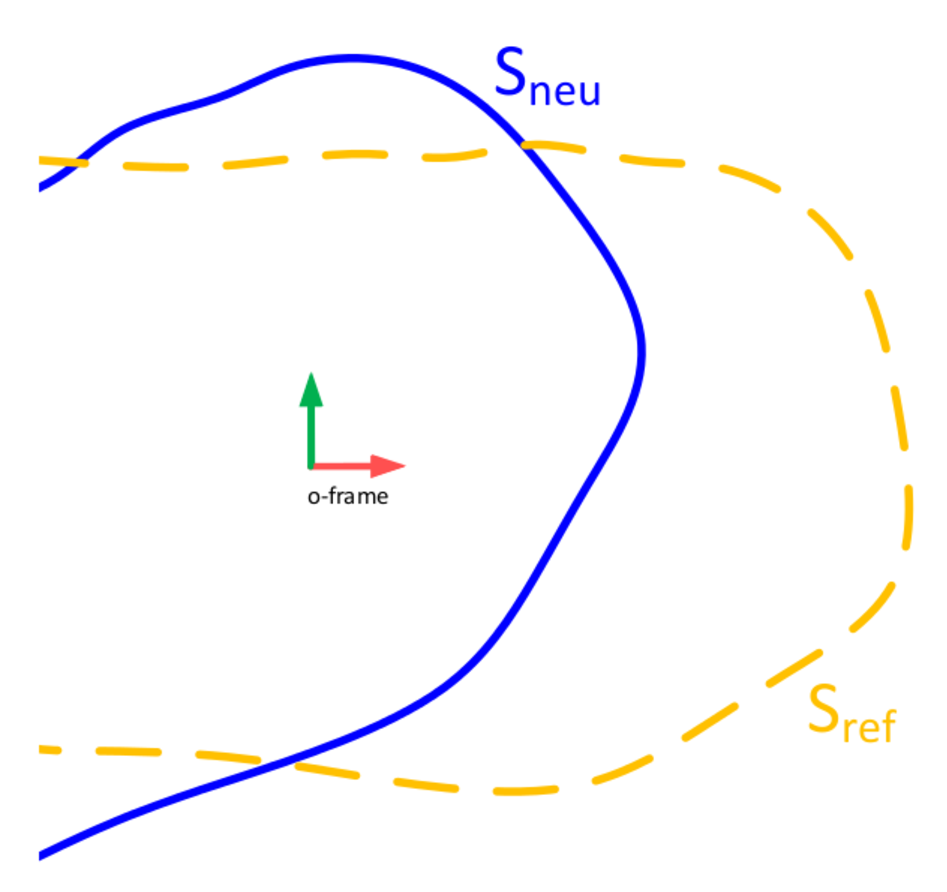
\includegraphics[width=0.4\textwidth]{images/scan_pose2d_a}
			\label{fig:scans_oframe}
		}
		\hspace{0.1\textwidth}
		\subfloat[Positon �ber Matching von $S_{neu}$ auf $S_{ref}$]{
			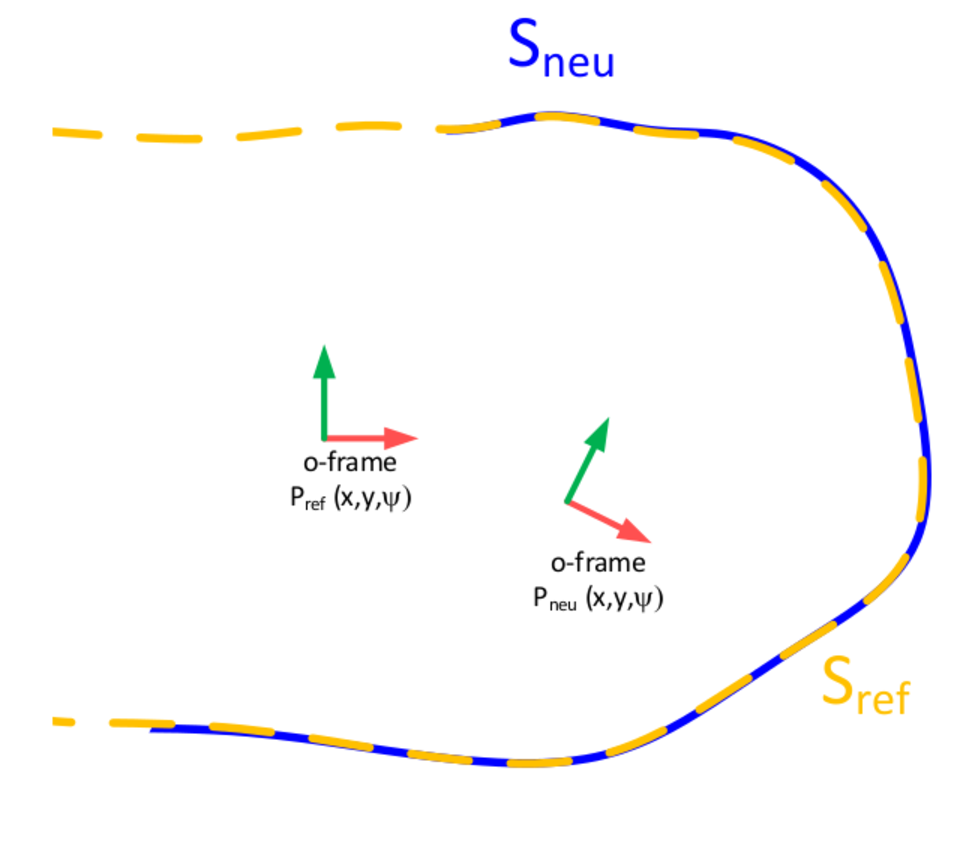
\includegraphics[width=0.4\textwidth]{images/scan_pose2d_b}
			\label{fig:scan_match}
		}
	}	
	\caption[Laserprojektion]{Prinzip Scanmatching}
	\label{fig:prinzip_scanmatching}
	
\end{figure}
Ausgangspunkt sind zwei im o-frame definierte Datenwolken. 
 \begin{equation}
 S_{ref} =[p_{ref_i} | i=1..n_{ref}]\\
 \end{equation}
 \begin{equation}
 S_{neu} =[p_{neu_i} | i=1..n_{neu}]  
 \end{equation}

Dargestellt in Abbildung \ref{fig:scans_oframe}. 

Zur Bestimmung des Matchings bzw. der Rotation $ M^o_z $ und der Translation $ T $ wurde im Jahr 1992 unter anderem von Paul Besl der \gls{icp}-Algorithmus entwickelt. Dabei handelt es sich um einen iterativen Algorithmus. Abgebildet sind die einzelnen Integrationsschritte in einem Flussdiagramm in Abbildung \ref{fig:icp_algorithmus}. Daran orientierend wird im folgenden jeder einzelne Vorgang erl�utert.

\begin{itemize}
	\item{
\underline{Vorgang 1,} Punktekorrespondenz.

 Hierbei bekommt jeder Punkt des $ S_{neu} $ einen korrespondierenden Punkt aus der Datenwolke $ S_{ref} $ zugewiesen. Man spricht hierbei von der Point-to-Point Arithmetik. Als Startwert werden als Korrespondenzpunkte die am n�chsten liegenden Nachbar �bergeben. Die Suche der entsprechenden Werte erfolgt �ber die Methode der ersch�pfenden Suche, d.h. jeden Punkt werden alle Punktast�nde ermittelt und der Punkt mit der geringsten Entfernung zugewiesen.  Das Ergebnis ist eine Datenmenge $ S'_{ref} $, deren Anzahl an Werten denen von $ S_{neu} $ entspricht.

\begin{equation}
S'_{ref} =[p'_{ref_i} | i=1..(n'= n_{neu})]\\
\end{equation}

Dieser Schritt stellt auf Grund des nicht optimierten Suchalgorithmus den rechenaufwendigsten Teil dar. Laut [LITERATUR AUT4] stellt dies f�r die Verarbeitung von 2D-Laserscans kein Problem dar.}

\item \underline{Vorgang 2,} Bestimmung des Rotationswinkel $\Delta\psi^o$ und der Translation $T$

Wie schon zu beginn angeklungen, soll eine rotatorische und translatorische Transformation zur �berlappung von $S_neu$ mit $S_ref$ f�hren. Idealit�t und eine sehr kleine �nderung vorausgesetzt k�nnte jeder Punkt von $ S_{neu} $ in den entsprechenden Punkt $ S_{ref}$ umgerechnet werden.

\begin{equation}
p_{ref_i} (M^o_z(\psi^o),T)) =  M^o_z(\psi^o) \cdot p_{neu_i}  + P_{ref} + T 
\label{eq:ideal_trans}
\end{equation}

Die Zweidimensionale Roationsmatrix $ M^o_z $ entspricht dabei der in Kapitel \ref{subsec:koordinatentransformation} eingef�hrten Koordinatentransformationsmatrix (\ref{eq:Mz}) reduziert auf die x und y Anteile. 

	\begin{equation}
M^o_z(\psi^o) = \begin{bmatrix}
	\cos\psi^o 	& -\sin\psi^o\\
	\sin\psi^o	& \cos\psi^o	\\
	
	\end{bmatrix}
	\label{eq:Mzo}
	\end{equation}



In der Praxis ist die Umgebung nicht ideal und aufgrund der hohen Dynamik k�nnen die �nderungen zwischen zwei Messwerten gr��er Ausfallen. Dadurch sind nicht alle Werte von $ S_{ref} $ und $ S_{neu} $ Indize f�r Indize vergleichbar. Der Grund warum in Vorgang~1 zu zum Scan $ S_{neu} $ ein korrespondier Scan $ S'_{ref} $ eingef�hrt wurde. Der im Folgenden Anwendung findet. Ein einsetzen von $ S'_{ref} $ in Gleichung (\ref{eq:ideal_trans}) ist jedoch nicht die L�sung des Problems, da es zu keiner eindeutigen Ergebnis f�hrt. Laut \cite{Lu94} kann aus dieser Formel (\ref{eq:ideal_trans}) als Fehlergleichung herangezogen werden. Mit dieser l�sst sich �ber die least-squar Methode die kleinste Summe der quadratischen Abweichungen ermitteln.

\begin{equation}
E(M^o_z(\Delta\psi^o),T) = \frac{1}{n'}\sum_{i=1}^{n'} ||p'_{ref_i}-( M^o_z(\Delta\psi^o)\cdot p_{neu_i} +T)||^2
 \label{eq:leastsquare}
\end{equation}

Um das Minimum  von abh�ngig $E(M^o_z(\Delta\psi^o),T)$ bestimmen zu k�nnen wird nach \cite{aut4} der Schwerpunkt ($c_{ref}$, $c_{neu}$) der korrespondierenden Punkte ermittelt.

\begin{equation}
c_{ref} = \frac{1}{n'}\sum_{i=1}^{n'} p'_{ref_i}
\end{equation}
\begin{equation}
c_{neu} = \frac{1}{n'}\sum_{i=1}^{n'} p_{neu_i}
\end{equation}

Damit ergibt sich die Datenwolken folgenderma�en beschreiben.

\begin{equation}
\tilde{S'}_{ref} = [\tilde{p'}_{pref_i} = p'_{pref_i} - c_{ref} |i=1..n']
\label{eq:Sref_tilde}
\end{equation}
\begin{equation}
\tilde{S}_{neu} = [\tilde{p}_{neu_i} = p_{neu_i} - c_{neu} |i=1..n']
\label{eq:Sneu_tilde}
\end{equation}

Setzt man \ref{eq:Sref_tilde} und \ref{eq:Sneu_tilde} in die Fehlergleichung \ref{eq:leastsquare} resultiert.
\begin{equation}
\begin{split}
 E(M^o_z(\Delta\psi^o),T) &= \frac{1}{n'}\sum_{i=1}^{n'} ||\tilde{p}_{ref_i}- M^o_z(\Delta\psi^o)\cdot \tilde{p}_{neu_i}-(T-c_{ref}+M^o_z(\Delta\psi^o)\cdot c_{neu} )||^2 \\
 &= \frac{1}{n'}\sum_{i=1}^{n'} ||\tilde{p}_{ref_i}- M^o_z(\Delta\psi^o)\cdot \tilde{p}_{neu_i}-\tilde{T}||^2
\end{split}
\end{equation}

�ber $\tilde{T}$ ist die Abweichung der Schwerpunkte translatorisch als auch rotatorisch beschrieben. Damit beide Schwerpunkte genau �ber einander liegen ist $\tilde{T} = 0$ zusetzen. Daraus ergibt sich.

\begin{equation}
0 = T-c_{ref}+M^o_z(\Delta\psi^o)\cdot c_{neu}
\label{eq:Ttilde0}
\end{equation}
    
und eine Fehlergleichung die nun mehr nur noch von der Rotation abh�ngig ist und dessen Betrag sich wie folgt darstellen l�sst. 

\begin{equation}
	\begin{split}
	E(M^o_z(\Delta\psi^o)) &= \frac{1}{n'}\sum_{i=1}^{n'} ||\tilde{p}_{ref_i}- M^o_z(\Delta\psi^o)\cdot \tilde{p}_{neu_i}||^2\\
	&= \frac{1}{n'}\sum_{i=1}^{n'} (\tilde{p}_{ref_i}^T\tilde{p}_{ref_i}+\tilde{p}_{neu_i}^T\tilde{p}_{neu_i}-2\tilde{p}_{ref_i}^T\cdot M^o_z(\Delta\psi^o)\cdot\tilde{p}_{neu_i})
	\end{split}	
\end{equation}

Weiterhin auf die Literatur \cite{aut4} beziehend ist es zur Minimierung von $E(M^o_z(\Delta\psi^o))$ ausreichend den gemischten Term zu $\tilde{E}(M^o_z(\Delta\psi^o))$ maximieren. 

\begin{equation}
\tilde{E}(M^o_z(\Delta\psi^o))_{max} = \underset{M^o_z(\Delta\psi^o)}{argmax} \hspace{.2cm} \sum_{i=1}^{n'} (2\tilde{p}_{ref_i}^T\cdot M^o_z(\Delta\psi^o)\cdot\tilde{p}_{neu_i})
\end{equation}

Beziehungsweise abh�ngig von $ \Delta\psi^o $.

\begin{equation}
\begin{split}
\tilde{E}(\Delta\psi^o)_{max} = \underset{}{argmax} \hspace{.2cm} \sum_{i=1}^{n'} (2(cos(\Delta\psi^o)(\tilde{x}_{ref}\cdot\tilde{x}_{neu}+\tilde{y}_{ref}\cdot\tilde{y}_{neu})\\+sin(\Delta\psi^o)(\tilde{y}_{ref}\cdot\tilde{x}_{neu}+\tilde{x}_{ref}\cdot\tilde{y}_{neu}))
\end{split}
\end{equation}

Aufgrund der trigonometrischen Addition besitzt der Summand eine Maximum f�r $ \Delta\psi^o $ wenn

\begin{equation}
\frac{\delta \tilde{E}(\Delta\psi^o)_{max} }{\delta (\Delta\psi^o) } = 0
\end{equation}

\begin{equation}
 \begin{split}
 0 = \hspace{.2cm} \sum_{i=1}^{n'} (-sin(\Delta\psi^o)(\tilde{x}_{ref}\cdot\tilde{x}_{neu}+\tilde{y}_{ref}\cdot\tilde{y}_{neu})\\+cos(\Delta\psi)^o(\tilde{y}_{ref}\cdot\tilde{x}_{neu}+\tilde{x}_{ref}\cdot\tilde{y}_{neu}))
 \end{split}
\end{equation}


draus folgt f�r $\Delta\psi^o $

\begin{equation}
\Delta\psi^o = \arctan(\frac{\sum_{i=1}^{n'}(\tilde{y}_{ref}\cdot\tilde{x}_{neu}+\tilde{x}_{ref}\cdot\tilde{y}_{neu})}{\sum_{i=1}^{n'}(\tilde{x}_{ref}\cdot\tilde{x}_{neu}+\tilde{y}_{ref}\cdot\tilde{y}_{neu})})
\label{eq:psio}
\end{equation}

Mit dem Ergebnis f�r $ \Delta\psi^o $ kann unter Verwendung von Gleichung \ref{eq:Ttilde0} die Translation T bestimmt werden.
\begin{equation}
T=c_{ref}-M^o_z(\Delta\psi^o)\cdot c_{neu}
\label{eq:T}
\end{equation}

Somit sind Translation und Rotation bestimmt.
 
\item\underline{Vorgang 3,} Ermittlung der Summe der quadratischen Fehler $E(M^o_z(\Delta\psi^o),T)$ 

Die aus der Formel \ref{eq:psio} stammende Rotation und die mit Hilfe der Gleichung \ref{eq:T} berechneten Translation werden in die Formel \label{eq:leastsquare} des quadratischen Fehlers eingesetzt.

\item\underline{Vorgang 4,} Vergleich von $E(M^o_z(\Delta\psi^o),T)$ mit Schwellwert $ E_{max} $ 

Der in Vorgang 4 berechnete quadratische Fehler wird mit dem Schwellwert des Maximal zul�ssigen Fehlers $ E_{max} $ verglichen. Wird unterschritten ist das Abbruchkriterium erf�llt,handelt es bei Rotation $ \Delta\psi^o $ und Translation $ T $ Werte die Transformation bzw. die neue Position $ P_{neu} $ mit einer ausreichenden Genauigkeit beschreiben. Ist das Kriterium beginnt der \gls{icp}-Algorithmus bei Vorgang 1 und bestimmt neue Korrespondenzen. 
\end{itemize}

\begin{figure}
	\centering
	
\includegraphics[width = .55\textwidth]{images/Platzhalter}
	\caption[l-frame]{Flussdiagram \gls{icp}-Algorithmus} %
	\label{fig:icp_algorithmus}
\end{figure}

F�r die Positionsbestimmung im n-frame wird mit der ersten Position $ P_{ref} $ der Bezugspunkt des Navigationskoordinatensystems gesetzt. Darauf aufbauend wird die weiteren Translationen bzw. Rotationen addiert. 

\begin{equation}
	P_{neu}= P_{ref}+T
\end{equation}
\begin{equation}
\psi^o_{neu}= \psi^o_{ref}+\Delta\psi^o
\end{equation}


Anzumerken sei hier das $ P_{ref} $ nicht im Ursprung verweilt, sondern sich auf den Refernzscan $ S_{ref} $ bezieht. Dieser kann der vorige Umlauf des aktuellen Scans $ S_{neu} $ darstellen. Oder einen in der nahen Vergangenheit liegenden Scan, bei dem die Summe der quadratischen Fehler sehr gering war.

Der vorgestellt \gls{icp}-Algorithmus kann weiterhin verbessert werden. So kann anstelle der Point-to-Point Arithmetik in Vorgang 1 eine Point-to-Line Arthmetik zur Ermittlung der Konvergenzpunkte angewendet werden. Mit diesem Thema besch�ftigt sich das Paper \cite{censi08plicp}. Au�erdem ist m�glich �ber die Inertialsenorik ausgehend von $ P_{ref} $ eine neue Position $ P_{imu} $ zu bestimmen. In $ P_{imu} $  wird der neue $ S_{neu} $ gelegt. So muss lediglich der Fehler der \gls{imu}-Positionssch�tzung �ber den \gls{icp}-Algorithmus eliminiert werden. Dies ist besonders n�tzlich wenn zwei Scans weit auseinander liegen, wie zum Beispiel in Abbildung \ref{fig:scan_match}. Es vereinfacht Vorgang 1. Behandelt wird dies unter anderem in \cite{Morris2010}.\\

Mit der Beschreibung Scanmatchingverfahren ist der letzte Baustein zur Lokalisierung des Quadrocopters in der horizontalen Ebene eines geschlossen Raum mittels eines 2D Laser geliefert worden. Darauf aufbauend ist es m�glich eine Positionsregelung zu implementieren.

%ANMERKUNG: DURCH VERWENDUNG DER IMU DATEN L�SST SICH EINE ERSTE POSITION SCH�TZEN SODASS 
%ES SEI DARAUF HINGEWIESEN DAS ES ALTERNATIVE ZUR PONIT ZU PONIT ARITHMETIK EINEN POINT TO LINE ARITHMETIK EXISTIERT
\chapter[Positionsregelung]{Verifizierung der Positionsregelung der ETH-Z�rich in Verbindung mit einem Laserscanner}
\label{chap:Positionsregelung}

In einer Zusammenarbeit von \gls{asctec} und der ETH-Z�rich wurde eine Regler zur Positionierung des Pelican Quadrocopters in geschlossenen R�umen entworfen und ver�ffentlicht. Der Entwurf basierte dabei auf einer monokularen Kamera �ber die mittels eines \gls{vslam}-Algorithmus und der Fusion der \gls{imu} die Position des Flugobjekts in der unbekannten Umgebung ermittelt wird. Regelung- und Fusionsalgortihmus sind im Paper \cite{Achtelik11} beschrieben. Aufgabe dieses Kapitel ist es die dort ver�ffentlichen Annahmen und Formel zu verifizieren. Dies erfolgt �ber Literaturrecherchen und Herleitung der publizierten Gleichungen. Unter Ber�cksichtigung, das die Position nun mehr vom Laser �ber die Kapitel \ref{chap:2Dpositionsbestimmung} vorgestellten Algortihmen bestimmt wird, ist Abschnitt \ref{sec:strukpositionsregelung} darauf ausgelegt eine �bersicht �ber die Bestandteile der Regelung zu geben. Herleitung der Komponenten erfolgt in den anschlie�end Unterkapiteln. 

%*************************************************************************************************************************
\section{Struktur der Positionsregelung}
\label{sec:strukpositionsregelung}
Das Hauptaugenmerk diese Unterkapitel liegt darauf, wie sich die Positionsregelung in die in Kapitel \ref{sec:Kommunikationsarchitekur} vorgestellte Systemstruktur einf�gt. Welche Softwarekomponenten daf�r auf dem \gls{hlp} integriert wurden. Wie die Kommunikation zwischen ihnen und der Umgebung aussieht. Mit dem Ziel ein grundlegendes Verst�ndnis f�r die Funktionsweise der Regelung zu generieren.\\
\begin{figure}
	\centering
	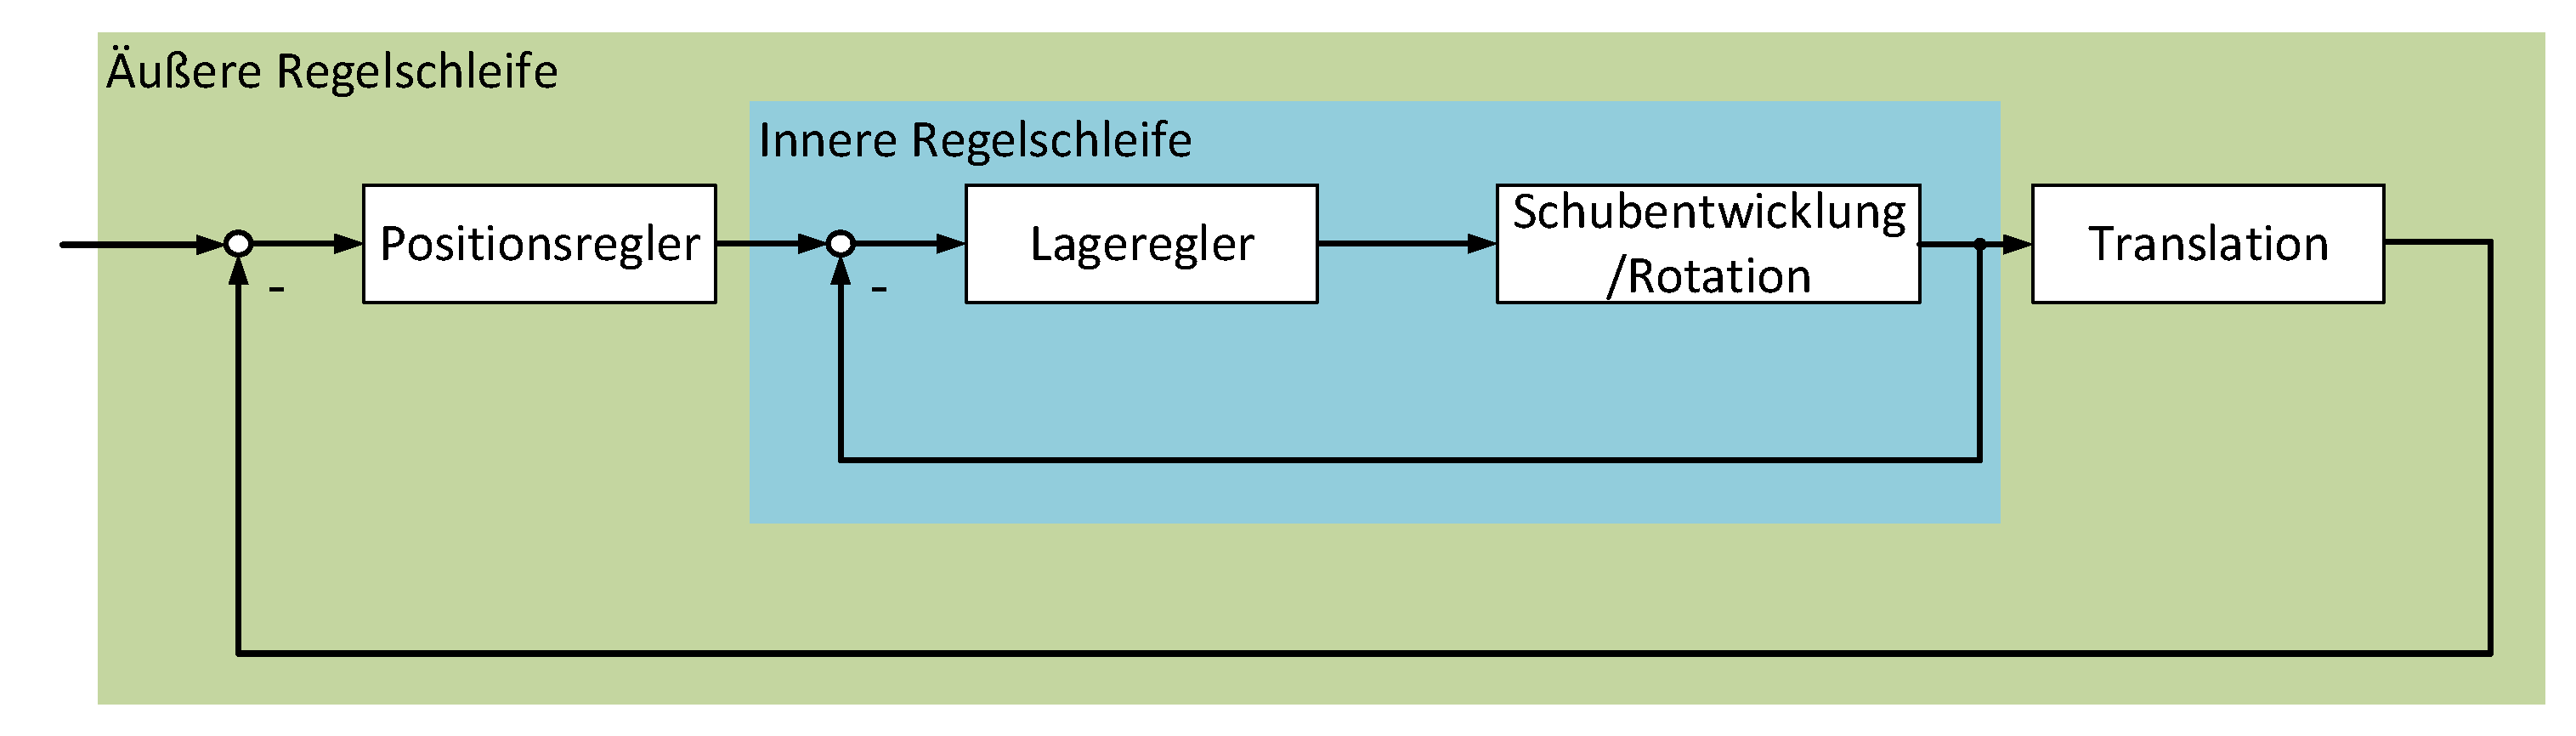
\includegraphics[width = .95\textwidth]{images/Kaskadenstruktur}
	\caption[Kaskadenstruktur]{Kaskadenstruktur der vereinfachten Positionsregelung } %
	\label{fig:kaskstruc}
\end{figure}


Die Positionsregelung wird auf die Lageregelung (engl. Attitudecontrol) aufgesetzt. Daraus resultiert eine Kaskadenstruktur (Abbildung \ref{fig:kaskstruc}). Diese Vorgehensweise ist nachvollziehbar, da die Lageregelung bereits Fest auf dem \gls{llp} implementiert ist. Diese besteht aus einem Regelalgorithmus der anhand der Regeldifferenz der Orientierung $e_{ori}$, resultierend aus der Abweichung Soll-Orientierung $O_{des}$ und Ist-Orientierung $ O  $, in Verbindung mit der Sollschubvorgabe $ T_s $ die Drehzahlen $ n_{1..4} $ der Rotoren berechnet und einstellt. Die Ist-Orientierung $ O =\begin{bmatrix} \phi&\theta&\psi\end{bmatrix}^T $ wird mittels eines Fusionsfilter bestimmt. Dieser fusioniert die Messwerte der auf der \gls{imu} befindlichen Gyroscope mit den Daten des 3D-Kompass. Wie dieser unterlagerte Regler und der dazugeh�rige Zustandssch�tzer genau ausgef�hrt sind ist nicht bekannt. Eine m�gliche Ausf�hrung ist in Paper \cite{hoffmann10} beschrieben. Die Ungewissheit �ber den Regleraufbau der Lageregelung stellt f�r den Entwurf der �berlagerten Positionsregelung kein Problem dar. Von Interesse ist lediglich, das die Annahme einer sehr hohen Dynamik dieses Reglers zur einer Vereinfachung des f�r die Positionsregelung ben�tigen Modells (Kapitel \ref{sec:Modelbildung}) f�hrt. Hohe Dynamik bedeutet, das der Sollwinkel in einer sehr kurzen Zeit $ t \rightarrow 0~s $ erreicht wird. Basierend auf einer Exakten Ein-/Ausgangslinearisierung der inneren Schleife (Kapitel \ref{sec:exkt.ealin}), ist die �u�ere Reglerschleife zur Positionsregelung auf dem \gls{hlp} realisiert. Dank der Inversion, realisiert Ein-/Ausgangslinearisierung, kann f�r die Positionierung des Quadrocopters eine linerare zwei Freiheitsgrade Regelung angewandt werden.
\begin{figure}
	\centering
	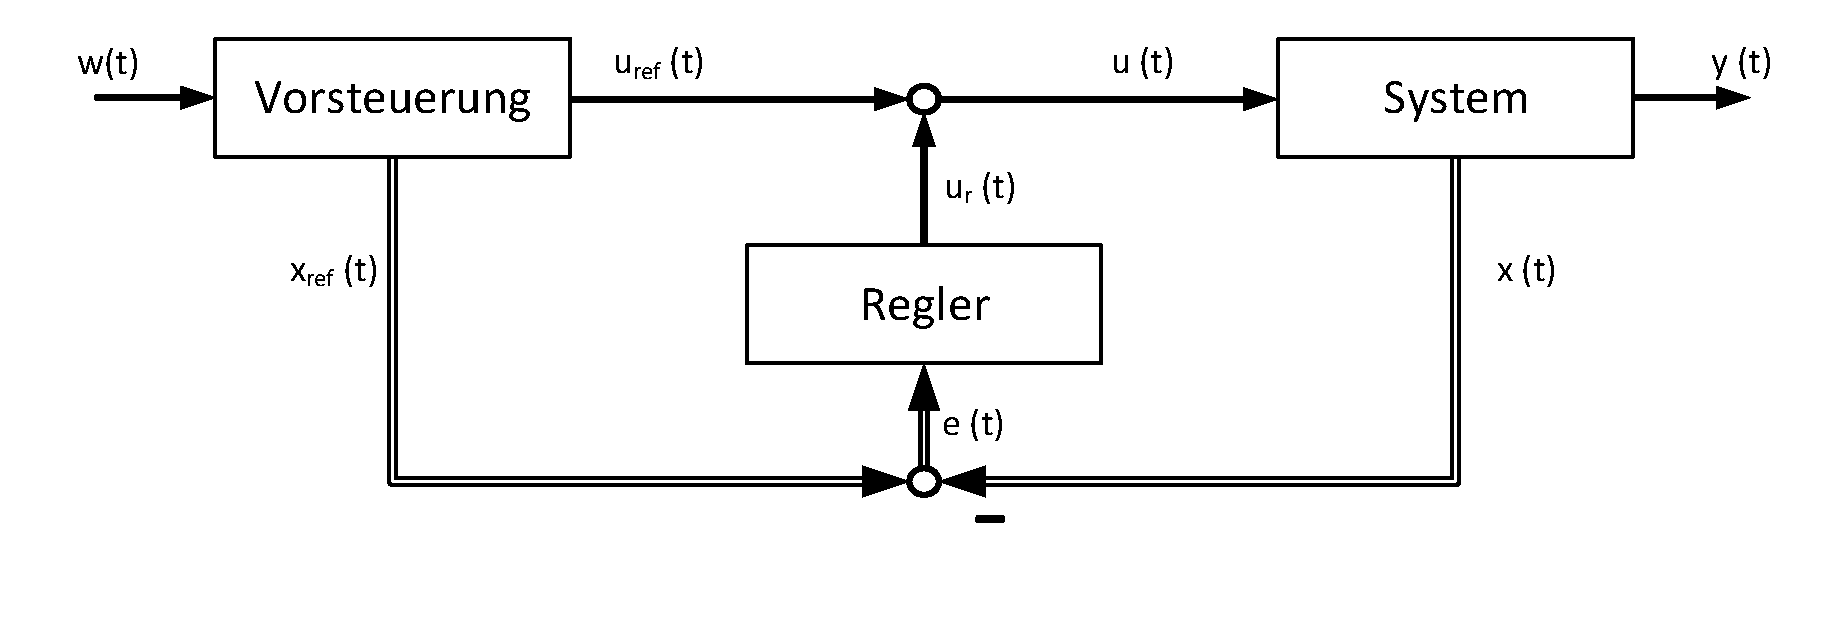
\includegraphics[width = .95\textwidth]{images/2-FHG-R}
	\caption[Gesamtstruktur Regelung]{Struktur zwei Freiheitsgraderegelung} %
	\label{fig:zweifgr}
\end{figure} Diese besteht aus einer Vorsteuerung und einem Folgeregler. Die Vorsteuerung auf dem \gls{hlp} ist in Form eines Referenzmodell (Kapitel \ref{sec:referenzmodell}), das dem Ein-/Ausgangslinearisierung nachempfunden ist, ausgef�hrt. Anhand der vorgegebenen Soll-Position $P^n_{des} = \begin{bmatrix} x&y&z\end{bmatrix}^T_{des} $ wird eine Referenz-Trajektorie \footnote{Trajektorien beschreiben einen zeitabh�ngigen Verlauf eines Wertes in einem Bezugssystem} zur �berf�hrung des Quadrocopters aus der aktuellen Ist-Position in die Soll-Position berechnet. Ergebnis ist ein Stellwert f�r die Inversion, der unter theoretischer Betrachtung die gew�nschte Bahnbewegung des Quadrocopters zur Ursache hat. In einem realen System ist dies durch ein Fl�sse der Umgebung, bsp. Wind nicht gew�hrleiste. Deshalb ist zus�tzlich der Folgeregler (Kapitel \ref{sec:folgeregeler}) implementiert, dessen Aufgabe besteht darin Abweichung der realen Zust�nde des Quadrocopters von den Referenzwerten auszuregelen. Die daf�r ben�tigten Zustandsgr��en des Flugsystems (Kapitel \ref{sec:Zustandsbestimmung}) werden durch die Fusion der in �ber den Laser bestimmten Position(Kapitel \ref{chap:2Dpositionsbestimmung}) mit den mit den Beschleunigungswerten der \gls{imu} ermittelt.

Bevor jede einzelne Komponente in den Folgekapiteln hergeleitet wird, ist in Abbildung~\ref{fig:strucregelung} die Verkn�pfung aller Komponenten noch einmal grafisch dargestellt.
\begin{figure}
	\centering
	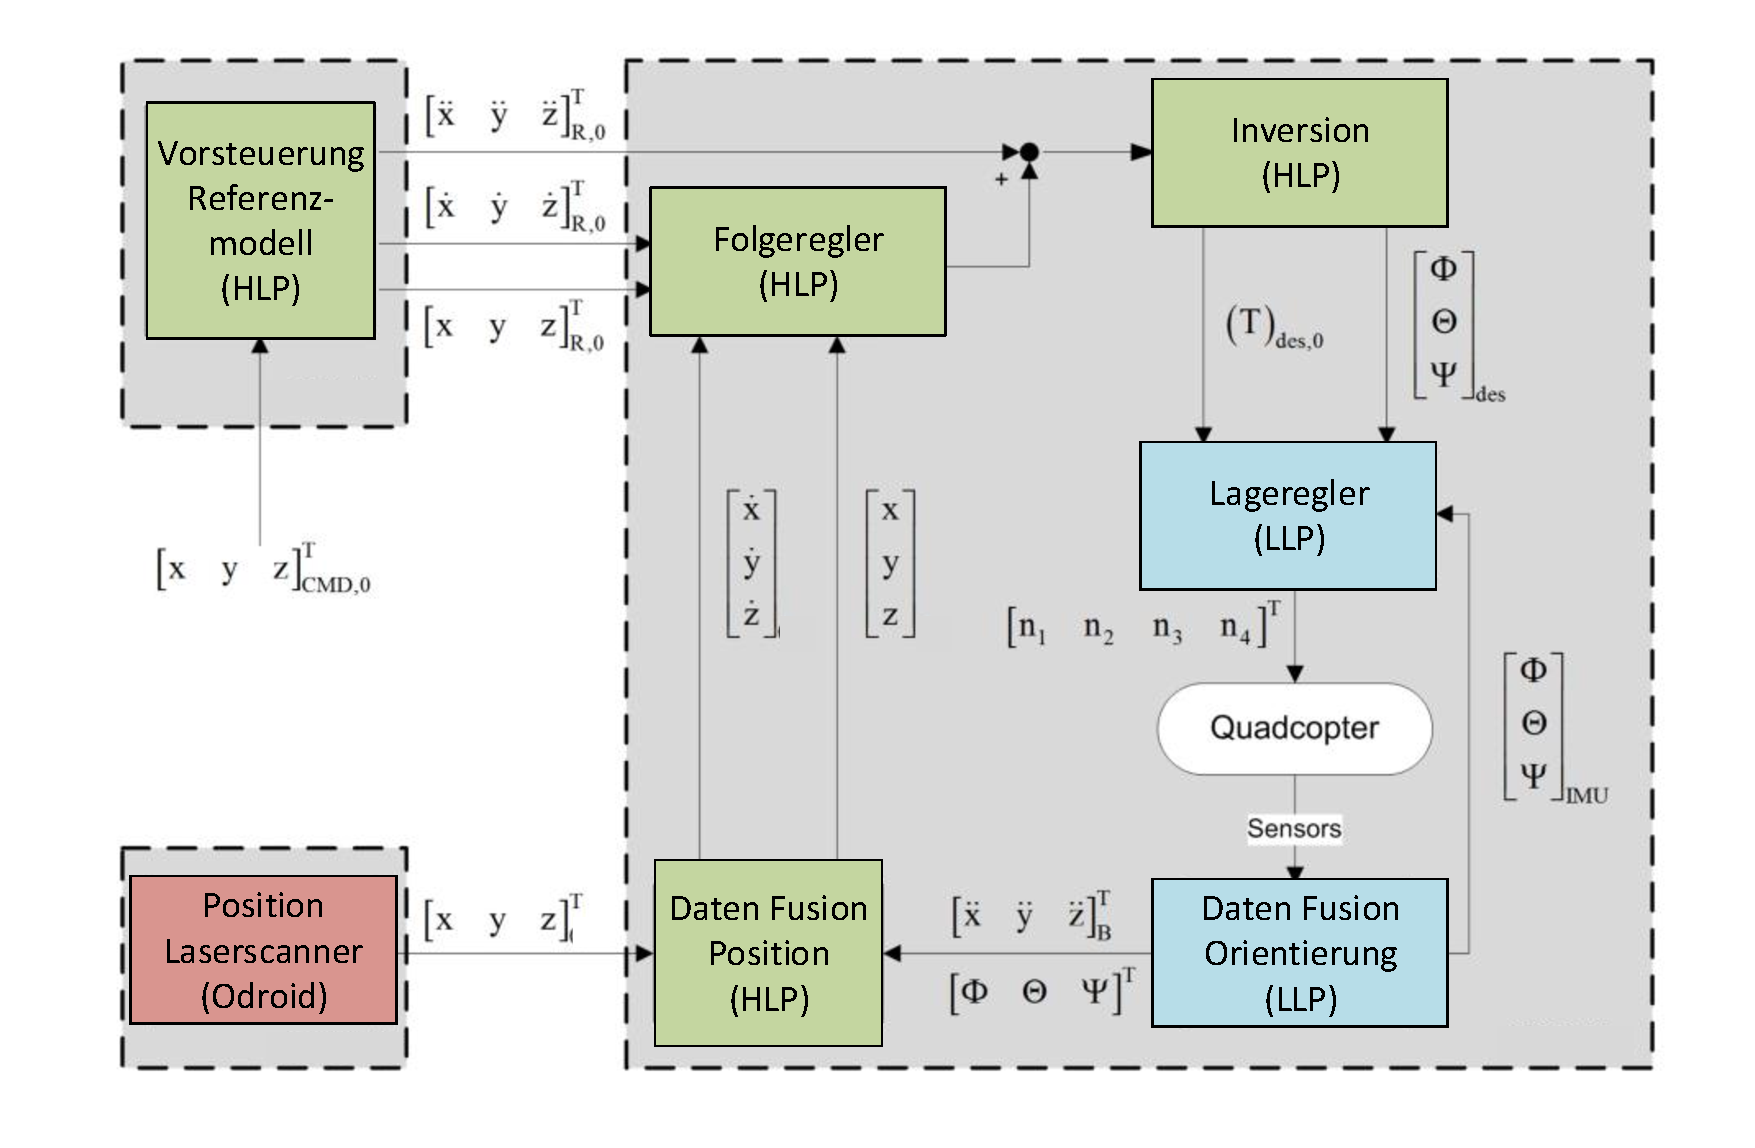
\includegraphics[width = .85\textwidth]{images/Reglerstruktur}
	\caption[Gesamtstruktur Regelung]{Struktur der Regelung} %
	\label{fig:strucregelung}
\end{figure}


Anzumerken ist, das die in Verbindung mit \gls{asctec} entworfene Positionsregelung, zur Ausrichtung des Quadrocopters in einem dreidimensionalen Raum entworfen ist. F�r die vertikale Positionierung ist jedoch in der vorrangegangen Arbeit\cite{JanKal13} von Jan Kallwies bereits eine Regelung entworfen worden. Da diese Regelung Effekte wie den Groundeffekt \footnote{In Bodenn�he verhindert der Untergrund das schnelle Abstr�men des durch die Rotoren erzeugten Luftstroms. Die daraus resultierende Krafterh�hung bei gleichbleibender Drehzahl der Rotoren, wird als Groundeffekt bezeichnet. } ber�cksichtigt, ist es Aufgabe einer dieser Arbeit folgenden Studentischen Projekt diese in das System der ETH-Z�rich einzupflegen. Somit reduziert sich die Validierung der Reglerstrukutur auf den horizontale Ebene. 

 

%*************************************************************************************************************************

\section{Modellbildung}
\label{sec:Modelbildung}
Die Modellbildung ist die Grundlage f�r den systematischen Entwurf einer Zustandsregelung. Dabei wird das Systemverhalten in Form von Differentialgleichungen abgebildet. Diese beschreiben die zeitliche Ver�nderung einer Ausgangsgr��e in Abh�ngigkeit ihrer zeitlichen Ableitungen sowie ver�nderlicher Eingangsgr��en. So lassen sich unter Beachtung der physikalischen Gesetze Bewegungsgleichungen aufstellen, welche das r�umliche und zeitliche Verhalten einen mechatronischen Systems abbilden. 

Bevor jedoch die Bewegungsgleichungen des Quadrocopter aufgestellt werden k�nnen, ist es notwendig die Freiheitsgrade des dynamischen Systems gegen�ber des Bezugssystem zu bestimmen. Da zwischen dem n-frame(Bezugssystem) und dem b-frame(Quadrocopter) keine mechanische Verbindung oder konstante Koordinatentransformation existiert besitzt das Flugsystem sechs Freiheitsgrade. Bestehend aus drei rotativen $\begin{bmatrix} \phi&\theta&\psi\end{bmatrix}^T$ und drei translatorischen $\begin{bmatrix} x&y&z\end{bmatrix}^T$. Sechs Freiheitsgrade sind gleichzusetzen mit sechs Differentialgleichungen zur Beschreibung der Bewegung im Raum. Damit ist jedoch nicht alle Dynamiken des Systems abgebildet. So sind zur Beschreiben des Gesamtsystems weitere Differentialgleichungen aufzustellen. Zum einen ist hier die Dynamik der Elektromotoren zu einzukalkulieren welche die Rotoren antreiben. Als auch die durch die Rotation der Rotorbl�tter ausgel�ste Schubentwicklung nach den Gesetzen der Str�mungslehre. Unter Beachtung aller Aspekte entsteht so eine mathematisch meist nichtlineare sowie sehr aufwendige und komplexe Systembeschreibung. Da mit der steigender Gr��e auch die Fehleranf�lligkeit steigt, wird in der Modellbildung folgender Leitsatz immer wieder aufgef�hrt. \glqq Ein Modell sollte das zu regelende Verhalten so einfach wie m�glich, aber so detailliert wie n�tig darstellen.\grqq  Betrachtet nun die Struktur des implementierten Flugregelung (Abbildung \ref{fig:strucregelung}) so l�sst sich das Modell aus Sicht der Positionsregelung stark reduzieren.  

Grund hierf�r ist die in Bild \ref{fig:kaskstruc} dargestellte Kaskadenstruktur der Regelung. In Verbindung mit Abbildung \ref{fig:strucregelung} ist zu erkennen, das der Lageregelung als Eingangsgr��en eine Soll-Orientierung $ O_{des} =\begin{bmatrix} \phi&\theta&\psi\end{bmatrix}^T $ und ein Schubvorgabe $T_{des}$ �bergeben wird. Aus Sicht der Positionsregelung sind dies auch die Eing�nge des zu regelnden Modells. Fest steht somit, das die rotative Dynamik als auch die Schubentwicklung �ber den auf dem \gls{llp} befindliche Regler eingestellt wird. Dieser ist ab Werk so gut parametriert, das die Zeitkonstante zwischen Vorgabe und Einstellen des Sollwerts sehr gering ist. Dies wurde auch durch einen Versuch best�tigt. Da der Aufbau der Lageregelung nicht bekannt ist wurde dazu das experimentelle Systemidentifikationstool von Manfred Ottens herangezogen. Um die Zeitkonstante sch�tzen zu k�nnen wurde das �bertagungsverhalten von Ist- zu Soll-Winkel als PT1-Glied abstrahiert. Aus den Messdaten des Sollwert und Istwert wurde daraus die Zeitkonstante T ermittelt. Dabei ergab das mittel �ber mehrere Messungen einen Zeitkonstante von T$\approx0.1~s$. Mit der Gewissheit, das die Dynamik der Positionsregelung um ein vielfaches geringer ausf�llt l�sst sich beim Entwurf dieser die Zeitkonstante T vernachl�ssigen. Es gilt somit Soll- entspricht Ist-Winkel.
 \begin{equation}
  O_{des} = O = \begin{bmatrix} \phi&\theta&\psi\end{bmatrix}^T
 \end{equation}
     
Somit reduziert sich die f�r Positionsregelung zu modellierende Dynamik auf die translatorische Differenzialgleichungen. Um zur Bestimmung dieser die Newtonsche Gesetze anwenden zu k�nnen, werden diese im n-frame definiert. Dabei kann der Quadrocopter als widerstandsfreie Kugel im dreidimensionalen Raum des Navigationskoordinatensystems abgebildet werden. Auf diese wirkt parallel zur z-Achse des n-frames die Gravitationskraft $ F^n_g $ und die in Richtung der $ z^b $-Achse angreifender Gesamtschub $ T $ (Gleichung \ref{eq:Schubvektor}) der Rotoren. Letzt genannte Kraft muss zur Anwendung der Newtonischen Gesetze in Kraftkomponenten des n-frames zerlegt werden (Abbildung \ref{fig:F_nframe}).
\begin{figure}
	\centering
	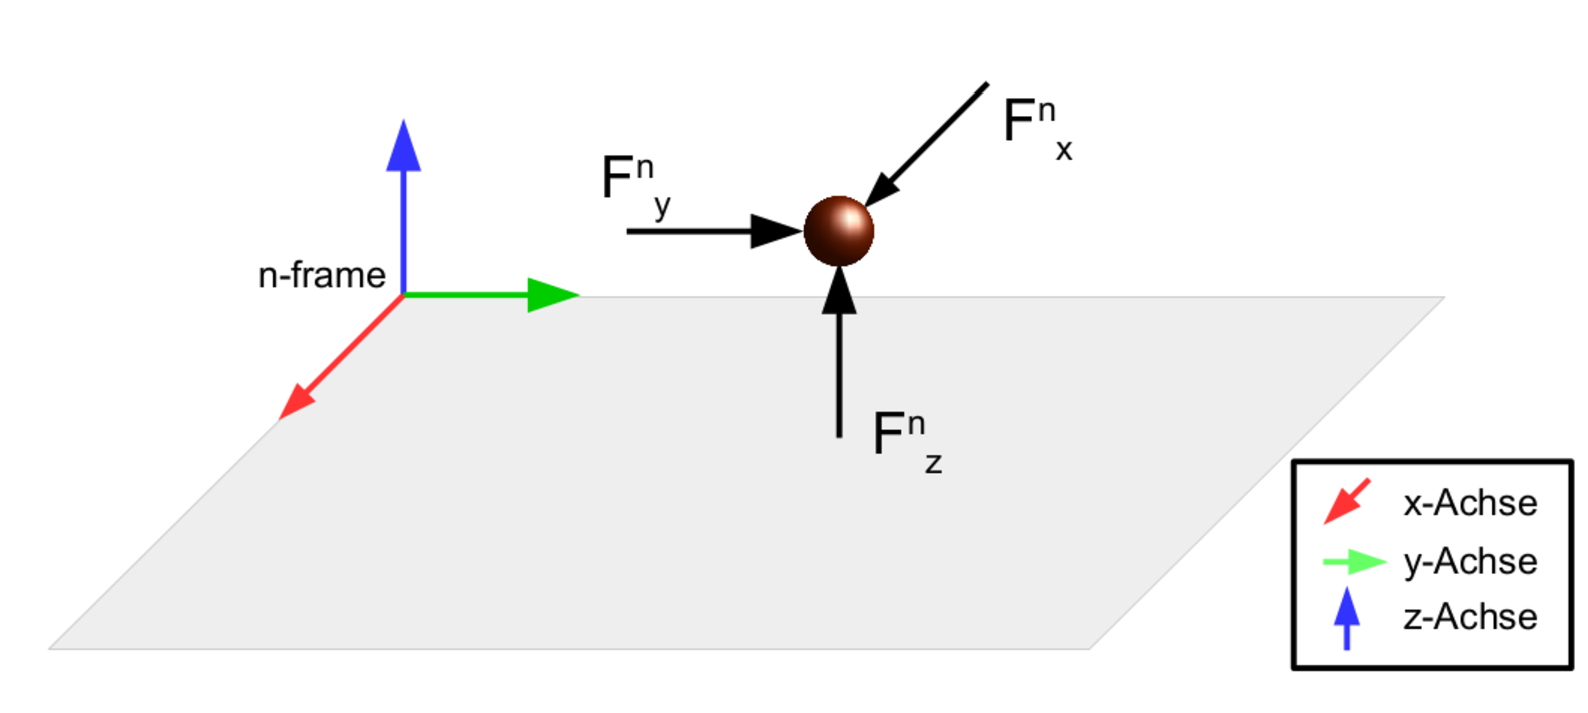
\includegraphics[width = .85\textwidth]{images/Force_nframe}
	\caption[]{Auf den Quadrocopter wirkende Kraft. Definiert im n-frame} %
	\label{fig:F_nframe}
\end{figure}     
Da die Dynamik der Lageregelung vernachl�ssigt wird, ist dies �ber eine einfache Koordinatentransformation vom b-frame ins n-frame realisierbar. Die entsprechende Transformation wurde in Kapitel \ref{subsec:koordinatentransformation} in Formel \ref{eq:inverse_transM} eingef�hrt. Daraus ergibt sich,

\begin{equation}
 F^n =	\begin{bmatrix}
	F^n_x \\
	F^n_y \\
	F^n_z \\
	\end{bmatrix}
	=
	M_{nb} \cdot F^b - F_g 
	=
	M_{nb} \cdot 
	\begin{bmatrix}
	0 \\
	0 \\
	T \\
	\end{bmatrix}
	-
	\begin{bmatrix}
	0 \\
	0 \\
	F_g \\
	\end{bmatrix}.
	\label{eq:superposF}
\end{equation} 
 
Nach dem zweiten Newtonschen Gesetz l�sst sich nun die Beschleunigung $ a $ des K�rpers bestimmen. Dieses besagt, eine �nderung der Bewegung resultiert proportional und gradlinig in Richtung der wirkenden Kraft. Dabei gilt die Beziehung. 
  
\begin{equation}
F^n =	\begin{bmatrix}
F^n_x \\
F^n_y \\
F^n_z \\
\end{bmatrix}
= m \cdot a = m \cdot	
\begin{bmatrix}
a^n_x \\
a^n_y \\
a^n_z \\
\end{bmatrix}
\label{eq:fma}
\end{equation} 

F�r die konstante Masse $ m (= 1.863~kg) $ des Quadrocoters, lassen sich die Beschleunigungen des K�rpers im dreidimensionalen Raum durch einsetzen von (\ref{eq:superposF}) in (\ref{eq:fma}) berechnen.
\begin{equation}
\begin{bmatrix}
a^n_x \\
a^n_y \\
a^n_z \\
\end{bmatrix}
=
\frac{1}{m} \cdot (
M_{nb} \cdot 
\begin{bmatrix}
0 \\
0 \\
T \\
\end{bmatrix}
-
\begin{bmatrix}
0 \\
0 \\
F_g \\
\end{bmatrix}
)
\label{eq:beschl}
\end{equation}

Basierend auf dem Weg-Zeit-Gesetz \cite{physik} l�sst sich f�r eine Anfangsgeschwindigkeit $ v^n_0  $ und eine Startposition $ P^n_0 $ die Position des Quadrocopters �ber die doppelte Integration der Beschleunigung aus Gleichung (\ref{eq:beschl}) bestimmen.
\begin{equation}
\begin{split}
a^n &= \dot{v}^n = \ddot{P}^n\\
v^n &= \dot{a}^n = \int a^n dt + v^n_0\\
P^n &= \int v^n dt + P^n_0
\end{split}
\label{eq:weg-zeit}
\end{equation}

Mit diesen Gleichung \ref{eq:weg-zeit} und \ref{eq:beschl} ist das translatorische Systemverhalten des Quadrocopters im n-frame mathematisch beschreibbar. Abh�ngig der Einganggr��en $ O_des $ und $ T_des $. Die resultierende Beschreibung der Zust�nde $ x =\begin{bmatrix}
v_x &
v_y &
v_z &
x &
y &
z 
\end{bmatrix}^T $ des Modells ergibt.
\begin{equation}
\begin{split}
\dot{x}_1 &= \frac{1}{m} \cdot ((\cos\phi\sin\theta\cos\psi+\sin\phi\sin\psi)\cdot T)\\
\dot{x}_2 &= \frac{1}{m} \cdot ((\cos\phi\sin\theta\sin\psi-\sin\phi\cos\psi)\cdot T)\\
\dot{x}_3 &= \frac{1}{m} \cdot ((\cos\phi\cos\theta)\cdot T)-g\\
\dot{x}_4 &= x_1\\
\dot{x}_5 &= x_2\\
\dot{x}_6 &= x_3\\
\end{split}
\label{eq:zstd}
\end{equation}
Zur Veranschaulichung ist das Modell zus�tzlich in Abbildung \label{fig:modstrukquad} visualisiert. 
\begin{figure}
	\centering
	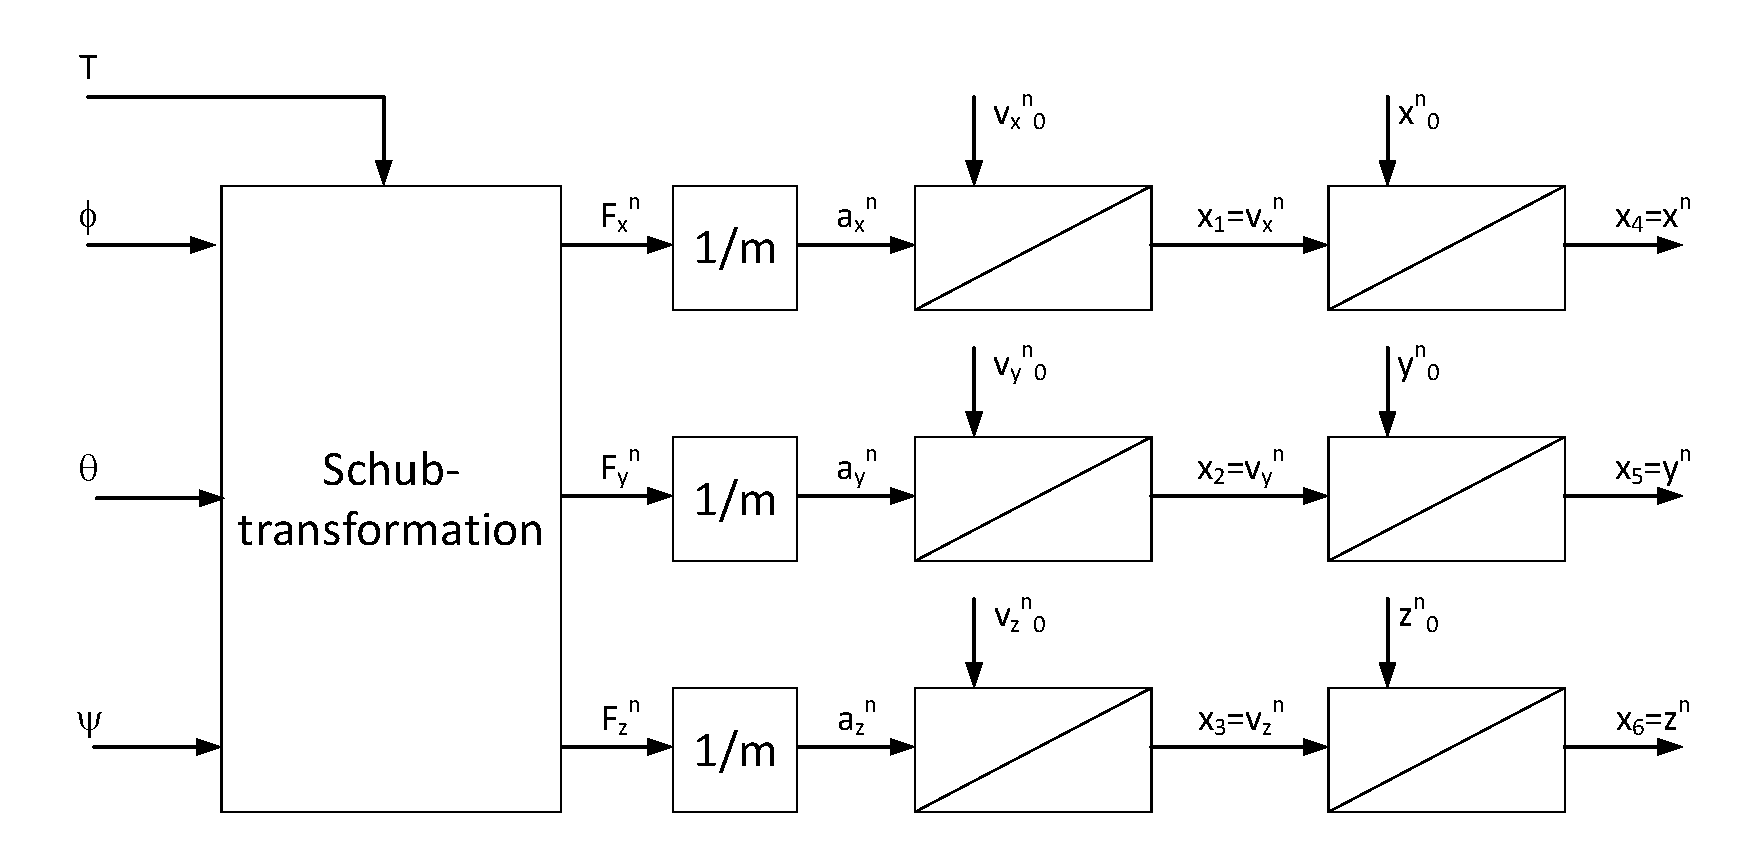
\includegraphics[width = \textwidth]{images/modell_lage_trans}
	\caption[]{Modellstruktur des Quadrocopters (FEHLER, GEWICHTSKRAFT FEHLT UND SUBTRANS ALS NICHTLINEAR MARKIEREN)} %
	\label{fig:modstrukquad}
\end{figure}

 
Durch die Koordinatentransformation bzw. die trigonometrichen Funktionen ist die Systembeschreibung nichtlinear. Das bedeutet, das von der �nderung der Eingangsgr��en keine direkt porportionale �nderung der Ausgangsgr��e ableitbar ist. Somit ist eine direkte Ansteuerung der Lageregelung �ber einen linearen Positionsregler nicht m�glich ist. Da allerdings einen ein solche linearer Regler vorgesehen ist, ben�tigt man einen Baustein. Der f�r fiktive Eing�nge das Systemverhalten linearisiert.    

%%++++++++++++++++++++++++++++++++++++++++++++++++++++++++++++++++++++++++++++++++++++++++++++

\section{Exakte Zustandslinearisierung}
\label{sec:exkt.zstdlin}
Zur Linearisierung eines nichtlinearen Modells wird in den Grundlagen der Regelungstechnik \cite{lunze08} die Arbeitspunktlinearisierung gelehrt. Nachteil eine solche Linearisierung besitzt oft nur f�r eine kleinen Umgebung um den Arbeitspunkt G�ltigkeit. Um mit dem Quadrocopter schnelle Positionswechsel vollziehen zu k�nnen, werden jedoch hohe Stellwinkel ben�tigt. Somit ist eine ann�hernde Linearisierung f�r einen Arbeitspunkt nicht ausreichend. Es wird daher eine Methode ben�tigt, die das Modell �ber den gesamten Arbeitsbereich linearisiert. 
\begin{figure}
	\centering
	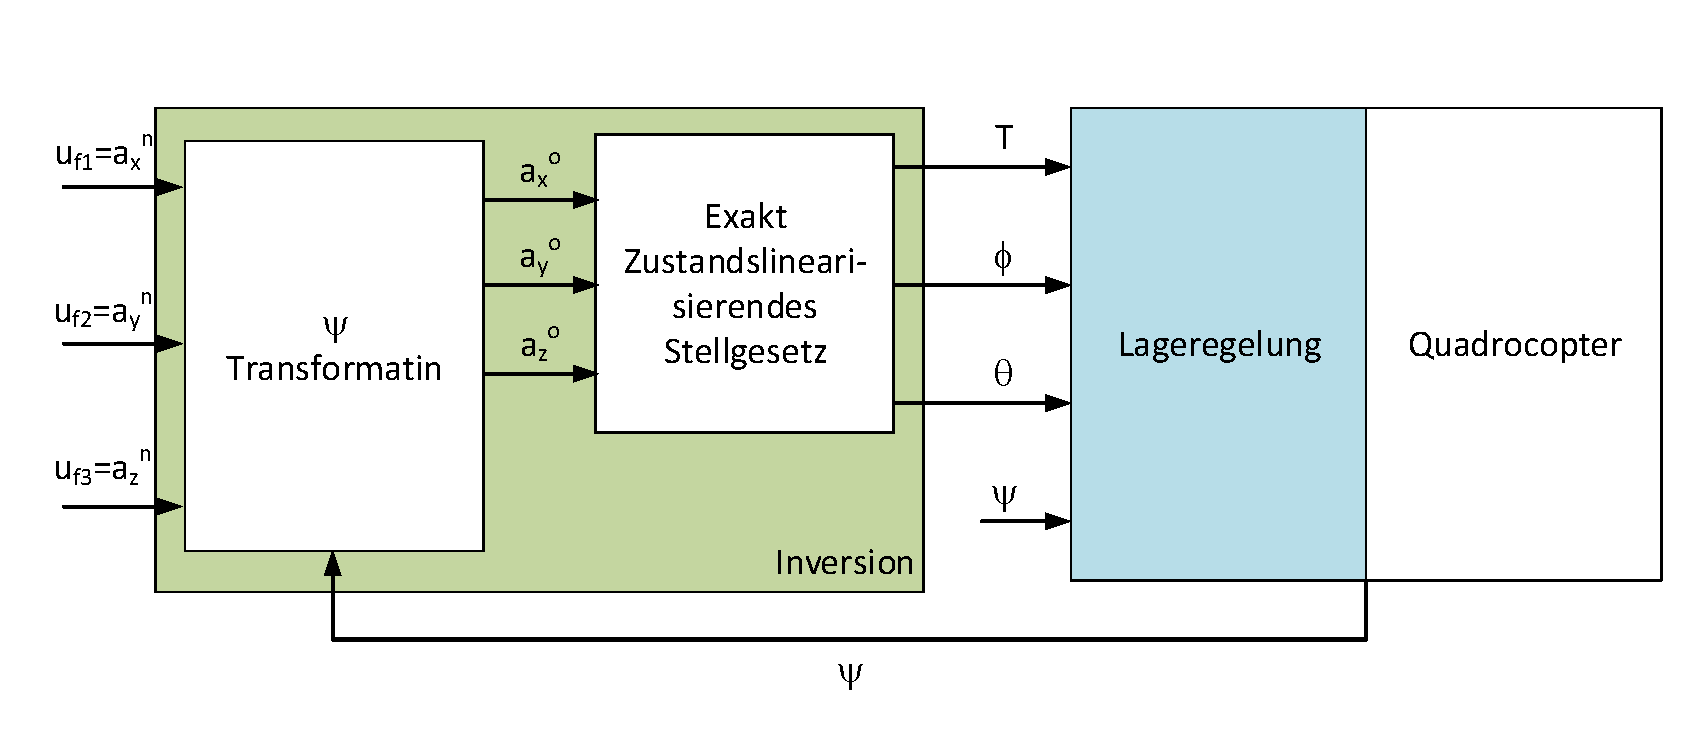
\includegraphics[width = \textwidth]{images/inversion}
	\caption[]{Gesamtinversion} %
	\label{fig:Gesamtinversion}
\end{figure} 

In \cite{deutNL} wird daf�r die exakte Zustandslinearisierung eingef�hrt. Dabei wird dem nichtlinearen System eine Inversion vorgeschaltet. Diese beinhaltet eine linearisierendes Stellgesetz so, dass sich das zu regelnde System f�r jeden Ausgang als entkoppelt und lineare Integrierekette darstellt. 

%Betrachtet man die Modellstruktur f�r die translatorische Bewegung (Abbildung \ref{fig:modstrukquad}) so kann man erkennen, das f�r fiktive Eing�nge $ u_f = \begin{bmatrix}
%a^n_x &
%a^n_y &
%y^n_z 
%\end{bmatrix}^T$ das Modell aus drei unabh�ngigen entkoppelten Integriererketten 2.Ordnung bestehen w�rde. Die per Definition der Linearit�t \cite{lunze08} ein lineares Zustandsverhalten aufweisen. Gesucht ist also ein Stellgesetz, das f�r die fiktiven Eing�ngen $ u_f $ die Stellgr��en der realen Eing�nge $ u = \begin{bmatrix} 
%T  &
%\phi &
%\theta &
%\psi 
%
%\end{bmatrix} $ generiert. Eine sogenannte Inversion. \\

Das bedeutet f�r das Quadrocoptermodell (Kapitel \ref{sec:Modelbildung}). Es ist ein Stellgesetz f�r $ u = \begin{bmatrix} T  &\phi &\theta &\psi \end{bmatrix} $ gesucht, welches das System f�r die Ausg�nge $ y =  \begin{bmatrix} 
x & y & z \end{bmatrix} $ entkoppelt. F�r die Positionsregelung steht so die fiktiven Eing�nge $u_f = \begin{bmatrix} a^n_x &	a^n_y & y^n_z \end{bmatrix}^T$ zur Verf�gung. Das bedeutet es k�nnen ohne Ber�cksichtigung der Orientierung des Quadrocopters Beschleunigungswerte im n-frame vorgegeben werden.

Damit eine solche Inversion f�r die Position als Ausgang $ y =  \begin{bmatrix}x & y & z & \end{bmatrix} $ m�glich ist, muss es sich bei diesem Ausgang um einen so genannten flachen Ausgang $ y_f = \begin{bmatrix} y_{f1} & y_{f2} & y_{f3} \end{bmatrix}$ handeln. 

%Vollst�ndige Definition siehe Anhang \ref{anh:def_fl}.  
%Damit aus dem nichtlinearen Modell Kapitel \ref{sec:Modelbildung} ein Exakt zustandslinearisierendes Stellgesetz (Inversion) generiert werden kann, muss es sich bei dem Ausgang $ y =  \begin{bmatrix} 
%x &
%y &
%z &  
%\end{bmatrix} $  um einen sogenannten flachen Ausgang $ y_f = \begin{bmatrix} 
%y_{f1} &
%y_{f2} &
%y_{f3} 
%\end{bmatrix}$ handeln. 

Per Definition (Anhang \ref{anh:def_fl}) muss daf�r das Kriterium, Anzahl der flachen Ausg�nge $ p_y $ entspricht der Anzahl der Eing�nge $ p_u $des nichtlinearen Systems, erf�hlt sein. Dieses ist f�r $ y_f = \begin{bmatrix} x & y & z \end{bmatrix}$ und die Eingangsgr��en $ u = \begin{bmatrix} T  & \phi & \theta & \psi \end{bmatrix} $ verletzt.
%kann es sich bei dem gew�nschten flachen Ausgang $ y_f = \begin{bmatrix} 
%x &
%y &
%z 
%\end{bmatrix}$ nur um einen solchen Handeln wenn die Anzahl der flachen Ausg�nge $ p $ derer der realen Eing�nge $ u $ entspricht. Dies ist nicht der Fall.
Nach \cite{deutNL} hei�t das, es muss ein neuer fiktiver Ausgang gesucht werden, sodass  $ p_y  = p_u$ gilt. Dieser neue Ausgang w�rde nicht mehr der Position entsprechen. Das bedeutet Positionsvorgaben m�ssten erst in die neuen Ausg�nge transformierten werden. Auch der gew�nschte fiktive Eingang der $u_f = \begin{bmatrix} a^n_x &	a^n_y & y^n_z \end{bmatrix}^T$ w�re nicht mehr gegeben.

Deshalb bedient sich die in Kooperation mit AscTec entwickelte Inversion \cite{Achtelik11} einem Trick.  
% Damit dennoch eine Inversion durchgef�hrt werden kann, ist es m�glich ein flacher Ausgang mit der selben Anzahl an Ausg�ngen wie Eing�ngen zu suchen. Dieser w�rde nicht mehr mit der Position $ P^n $ �bereinstimmen. Deshalb wurde in Paper \cite{Achtelik11} ein anderer Weg eingeschlagen.  
Um die Position als flachen Ausgang zu erhalten, bedient man sich der Tatsache, das eine Ver�nderung des $ \psi $-Winkels zu keiner Auslenkung des Schubvektors $ T $ f�hrt. So k�nnen die Beschleunigungsvorgaben $ u_f $ �ber eine einfache Transformation (Gleichung \ref{eq:Mz}) um den Winkel $ \psi $ ins o-frame �bertragen werden $\tilde{u}_f = \begin{bmatrix} a^o_x &	a^o_y & y^o_z \end{bmatrix}^T$. Gleiches gilt auch f�r den zugeh�rigen Ausgang $ y_f $. Somit ergibt sich f�r diesen $\tilde{y}_f = \begin{bmatrix} y^o_{f1} &	y^o_{f2} & y^o_{f2} \end{bmatrix}$.Durch diesen Trick reduziert sich die Anzahl der Eing�nge der f�r Inversion um einen. So entspricht die Anzahl der verbliebenen Eing�ngen $ \tilde{u} = \begin{bmatrix} \phi & \theta & T \end{bmatrix} $ denen des gew�nschten flachen Ausgangs. Damit ist die Flachheit des Ausgangs $ \tilde{y}_f $ nicht erwiesen. Es fehlt per Definition (vgl. Anhang \ref{anh:def_fl}) noch der Beweis, das sich alle Zust�nde $ \tilde{x} $ (vgl. Abbildung \ref{fig:modstrukquad}) und die reduzierten Eing�nge $ \tilde{u} $ durch die flachen Ausg�nge $ \tilde{y}_f $ und dessen Ableitungen darstellen lassen. F�r die Zust�nde ist dieser Beweis, ohne gro�en Rechenaufwand m�glich.

\begin{equation}
\begin{split}
\tilde{y}^o_{f1} &= x^o = x_4 \\
\tilde{y}^o_{f2} &= y^o = x_5 \\
\tilde{y}^o_{f3} &= z^o = x_6 \\
\\\dot{\tilde{y}}^o_{f1} &= \dot{x}^o = x_1 \\
\dot{\tilde{y}}^o_{f2} &= \dot{x}^o = x_2 \\
\dot{\tilde{y}}^o_{f3} &= \dot{z}^o = x_3 
\end{split}
\end{equation}

F�r die Eingangsgr��en $ \tilde{u} $ m�ssen die Zustandsgleichungen f�r $ \dot{\tilde{x}}_1$, $ \dot{\tilde{x}}_2 $ und $ \dot{\tilde{x}}_3 $ (vgl. Gleichung \ref{eq:zstd}) nach $ \phi $, $ \theta $ und $ T $ aufgel�st werden. Dabei entspricht $ \dot{\tilde{x}}_1 = a^o_x = \ddot{\tilde{y}}_{f1} = \tilde{u}_{f1}$, $ \dot{\tilde{x}}_2 = a^o_y = \ddot{\tilde{y}}_{f2} = \tilde{u}_{f2}$ sowie $ \dot{\tilde{x}}_3 = a^o_z = \ddot{\tilde{y}}_{f3} = \tilde{u}_{f3}$. Damit kann der Schub $ T $ als Betrag der im o-frame wirkenden Kr�fte, bzw. geforderten Beschleunigungen multipliziert mit der Masse dargestellt werden.

\begin{equation}
\begin{split}
T &= m \cdot \sqrt{\ddot{\tilde{y}}_{f1}^2 +\ddot{\tilde{y}}_{f}^2+(\ddot{\tilde{y}}_{f3}+g )^2 }\\
&= m \cdot \sqrt{{a^o_x}^2 +{a^o_y}^2+(a^o_z+g)^2}
\end{split}
\label{eq:invT}
\end{equation}    

Nun da $ T $ bestimmt, ist unter Beachtung das $ \psi = 0 $, durch die vorgelagerte Transformation, $ \dot{\tilde{x}}_2 $ aus  Gleichung \ref{eq:zstd} nach  $ \phi $ aufzul�sen. Damit ergibt sich,

\begin{equation}
\begin{split}
\phi &= -\arcsin(\frac{\ddot{\tilde{y}}_{f2}\cdot m}{T})\\
& = -\arcsin(\frac{a^o_y\cdot m}{T}).
\end{split}
\label{eq:invphi}
\end{equation}

$ \theta $ l�sst sich aufgrund der trigonometrischen Beziehung $ tan\alpha = \frac{\sin\alpha}{\cos\alpha} $ aus den Zustandsgleichungen f�r $ \dot{\tilde{x}}_1 $ und $ \dot{\tilde{x}}_3 $ berechnen.
\begin{equation}
\begin{split}
\theta &= \arctan(\frac{\ddot{\tilde{y}}_{f1}}{\ddot{\tilde{y}}_{f3}+g})\\
&=\arctan(\frac{a^o_x}{a^o_z+g})
\end{split}
\label{eq:invtheta}
\end{equation}

\begin{figure}
	\centering
	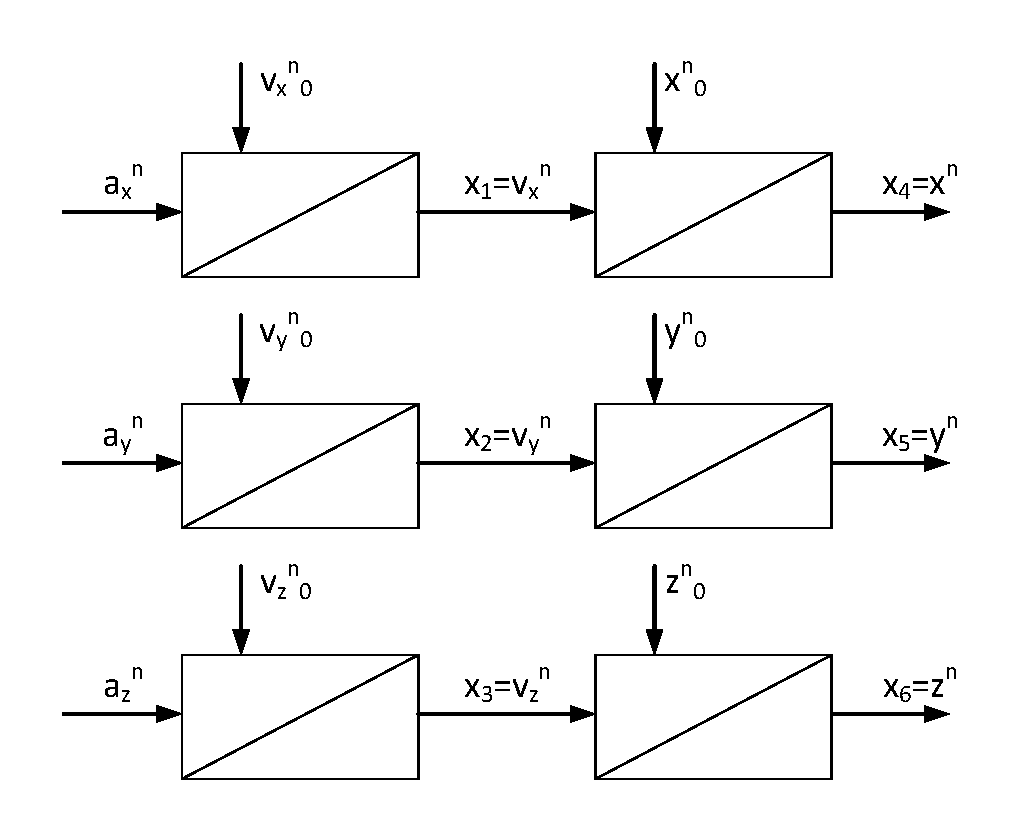
\includegraphics[width = .85\textwidth]{images/3intket}
	\caption[]{Modell aus Sicht der Positionsregelung dank Inversion} %
	\label{fig:drIntket}
\end{figure}

Die Stellgesetze der exakten Zustandslinearisierung sind damit �ber Gleichung (\ref{eq:invT}), (\ref{eq:invphi}) und (\ref{eq:invtheta}) mathematisch beschrieben. In Verbindung mit der Koordinatentransformation von $ \psi $ ergibt sich die in Abbildung \ref{fig:Gesamtinversion} dargestellte Inversion.

Die Richtigkeit dieser l�sst sich �ber eine Simulation beweisen. Das Modell besteht dabei aus Inversion (Abbildung \ref{fig:Gesamtinversion}) und Translationsmodell (Abbildung \ref{fig:modstrukquad}). �ber den neuen Eingang $ u_f $ werden dabei Beschleunigungswerte im n-frame vorgegeben (Abbildung \ref{fig:inv_uf}). Unter Einfluss st�ndig wechselnden  
Orientierung um die Hochachse (Abbildung ), ergeben sich die in Abbildung dargestellten Vorgaben f�r das Exaktzustandslineariesierden Stellgesetz. Die daraus resultierende Schubvorgabe und Winkel werden dem Bewegungsmodell �bergeben. Mit dem Ergenis, das die resultierendne Beschleunigungen des Modells denn Beschleunigunsvorgaben entspricht.

Dadurch kann nun das zu regelnde System als lineares Modell bestehend aus drei entkoppelten Integrierketten (Abbildung \ref{fig:drIntket}) gesehen werden. Dieses System ist jedoch instabil. Das bedeutet, f�r Vorgabe einer konstanten Beschleunigung, schwingt der Quadrocopter auf keiner konstanten Position ein, sondern Integriert seine Position immer weiter auf. Begr�ndet ist diese Verhalten auch durch das Weg-Zeit-Gesetz (Gleichung \ref{eq:weg-zeit}). M�glich ist es jedoch einen Beschleunigungsverlauf vorzugeben, f�r den der Quadrocopter in eine neue Position �berf�hrt wird. Daf�r ben�tigt wird eine Vorsteuerung.


 \begin{figure}
 	
 	\centering{
 		\subfloat[Neue fiktive Eing�nge]{
 			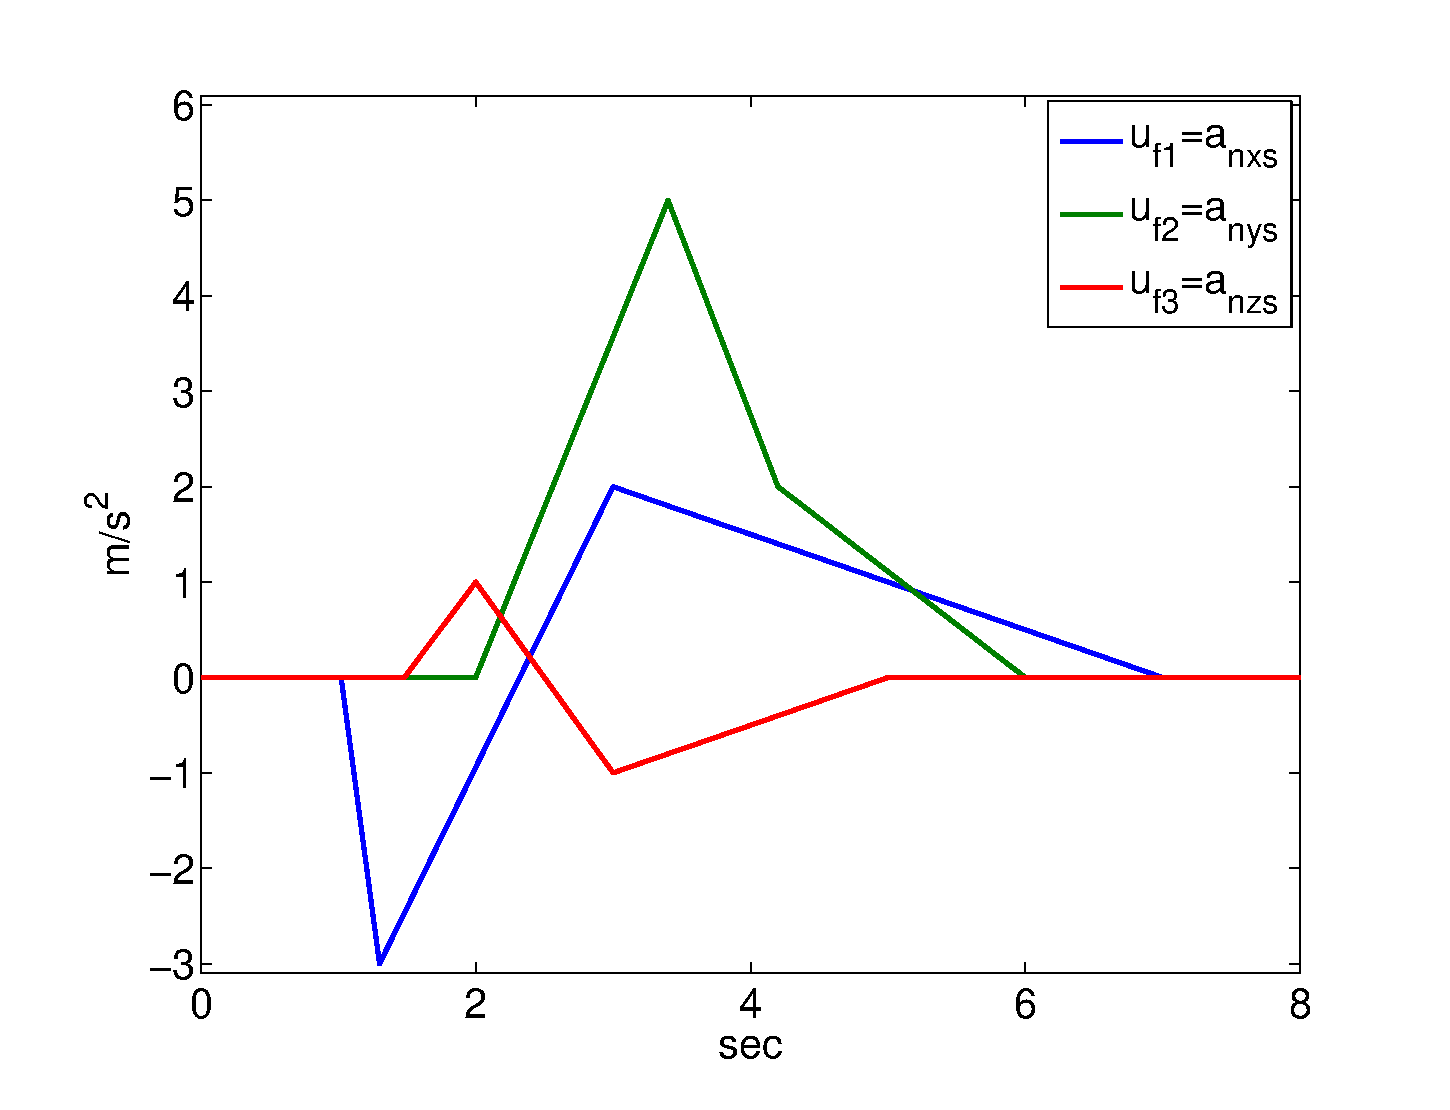
\includegraphics[width=0.5\textwidth]{images/inv_uf}
 			\label{fig:inv_uf}
 		}
 		\subfloat[Orientierung um z-Achse]{
 			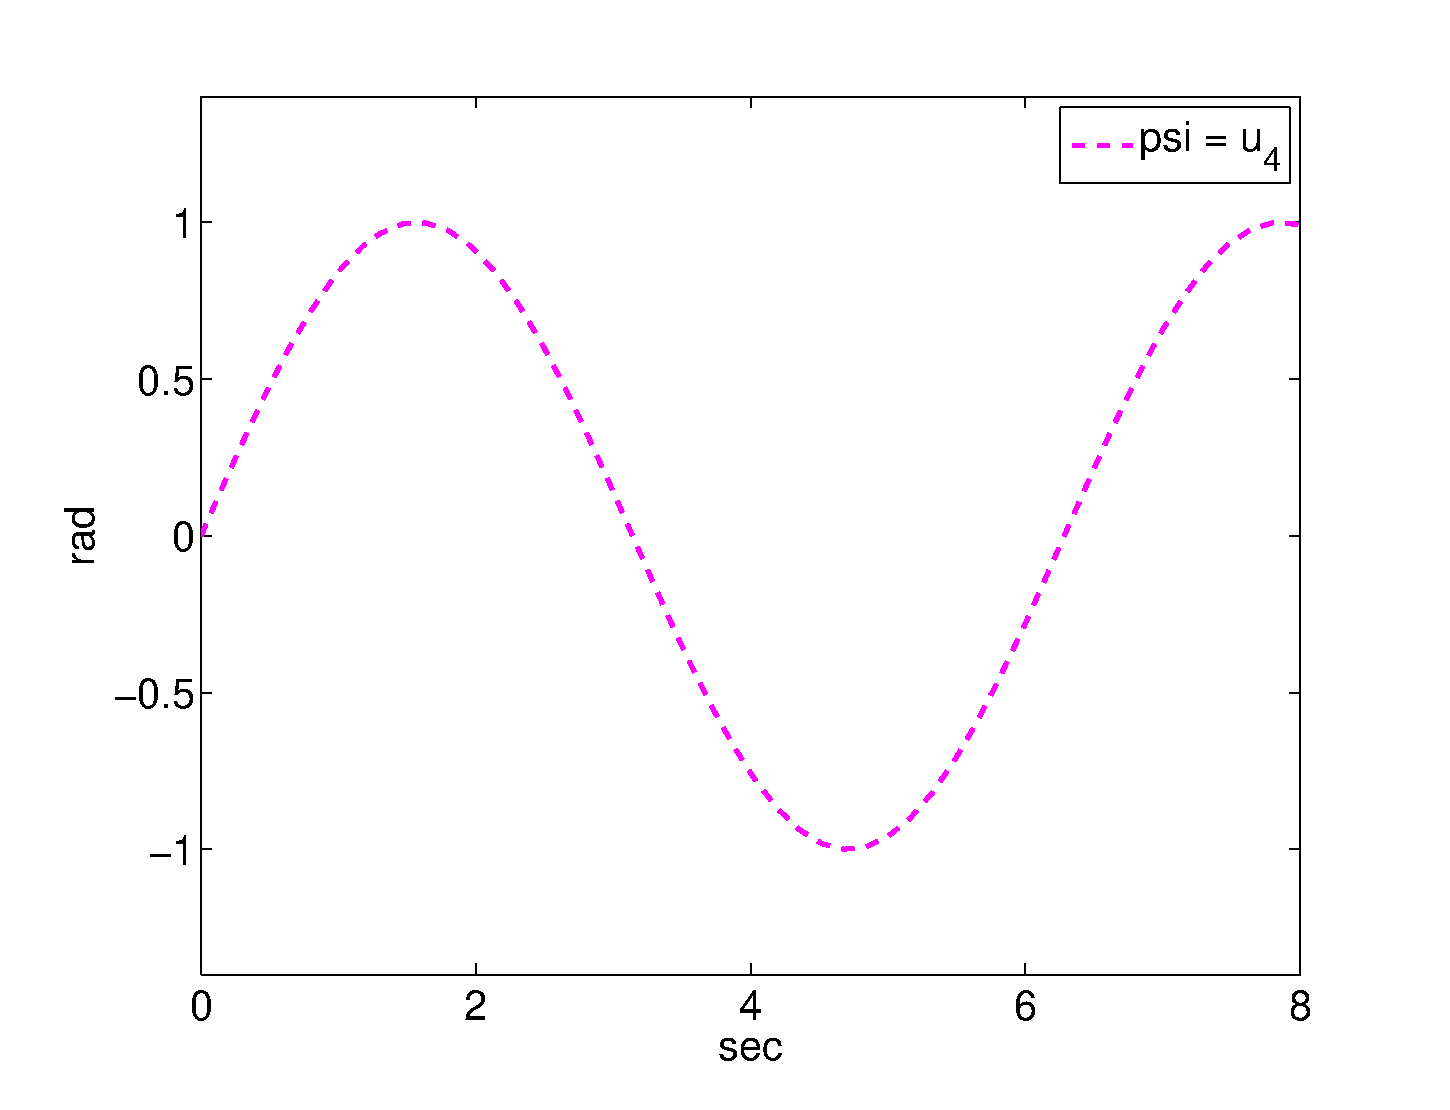
\includegraphics[width=0.5\textwidth]{images/inv_psi}
 			\label{fig:inv_psi}
 		}\\
 		\subfloat[Ins o-frame transformierte Beschleunigungsvorgaben]{
 			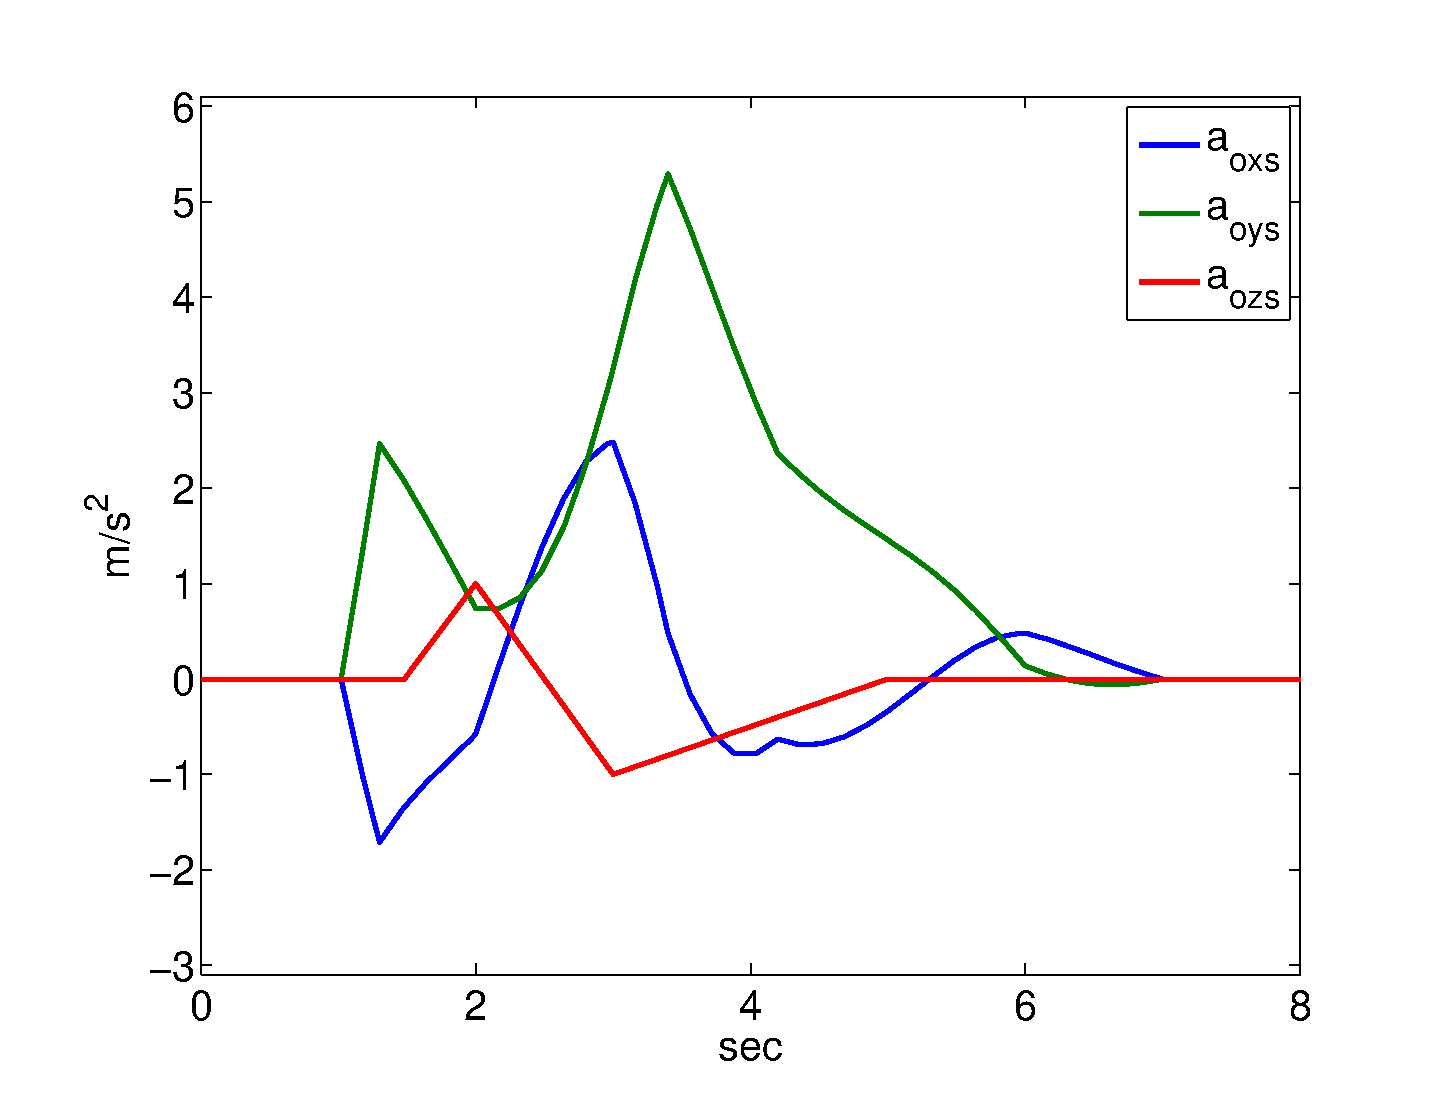
\includegraphics[width=0.5\textwidth]{images/inv_aso}
 			\label{fig:inv_aso}
 		}
 		\subfloat[Schubvorgabe der Inversion]{
 			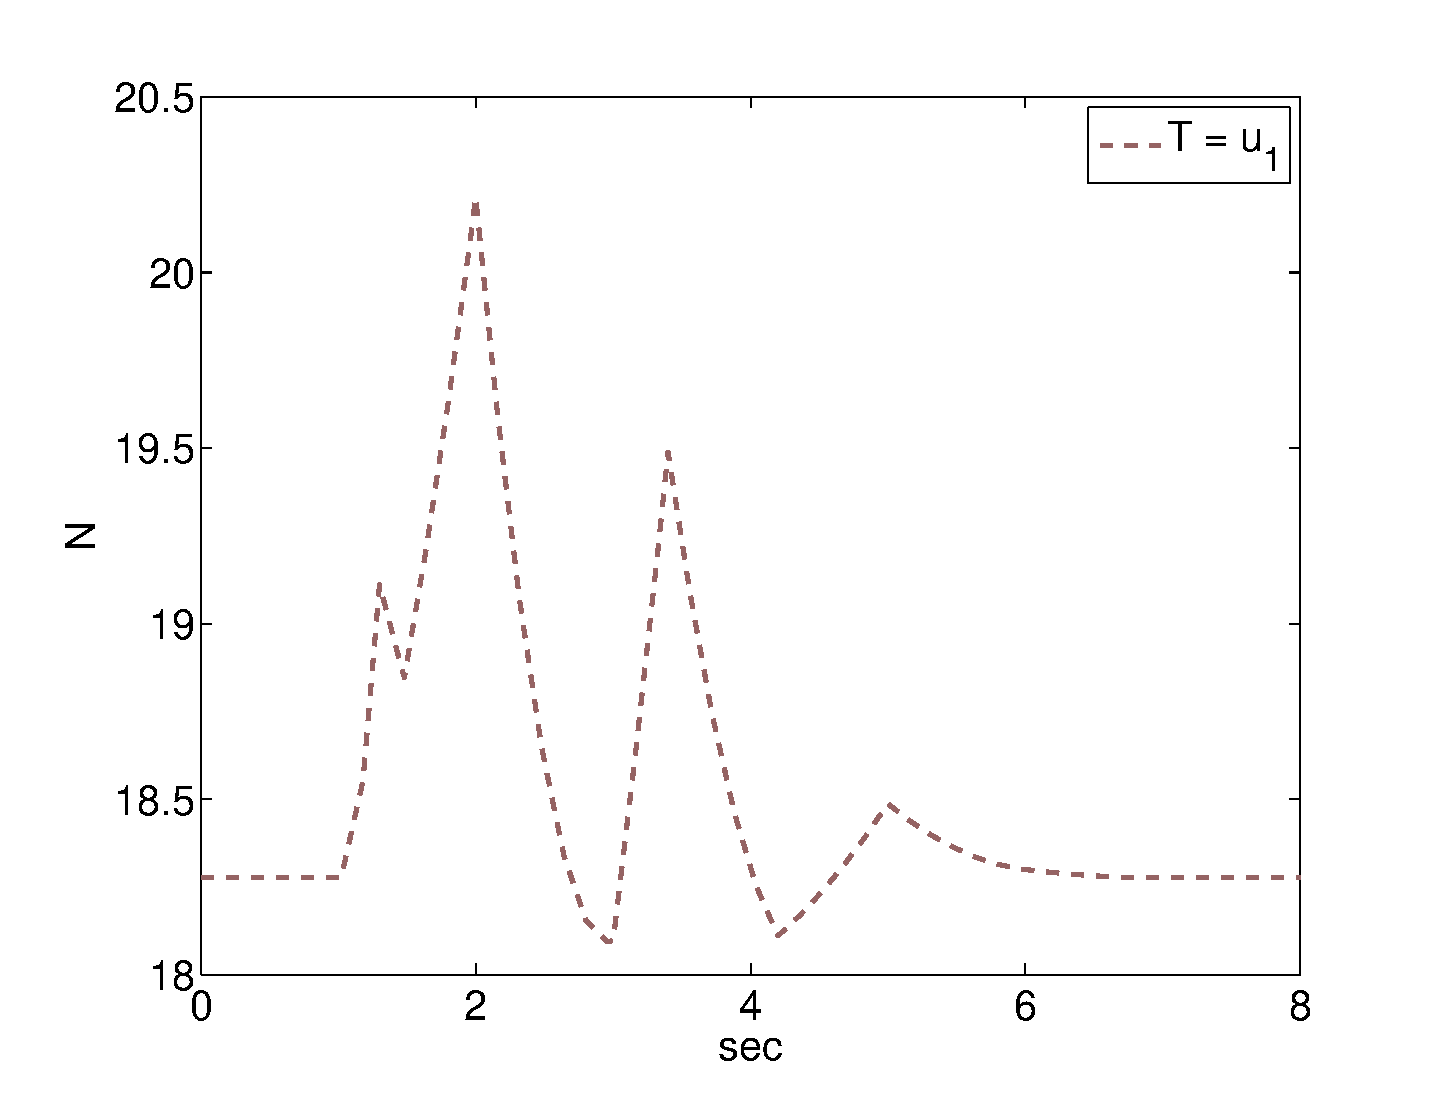
\includegraphics[width=0.5\textwidth]{images/inv_T}
 			\label{fig:inv_T}
 		}\\
 		\subfloat[Sollwinkel f�r die Lageregelung]{
 			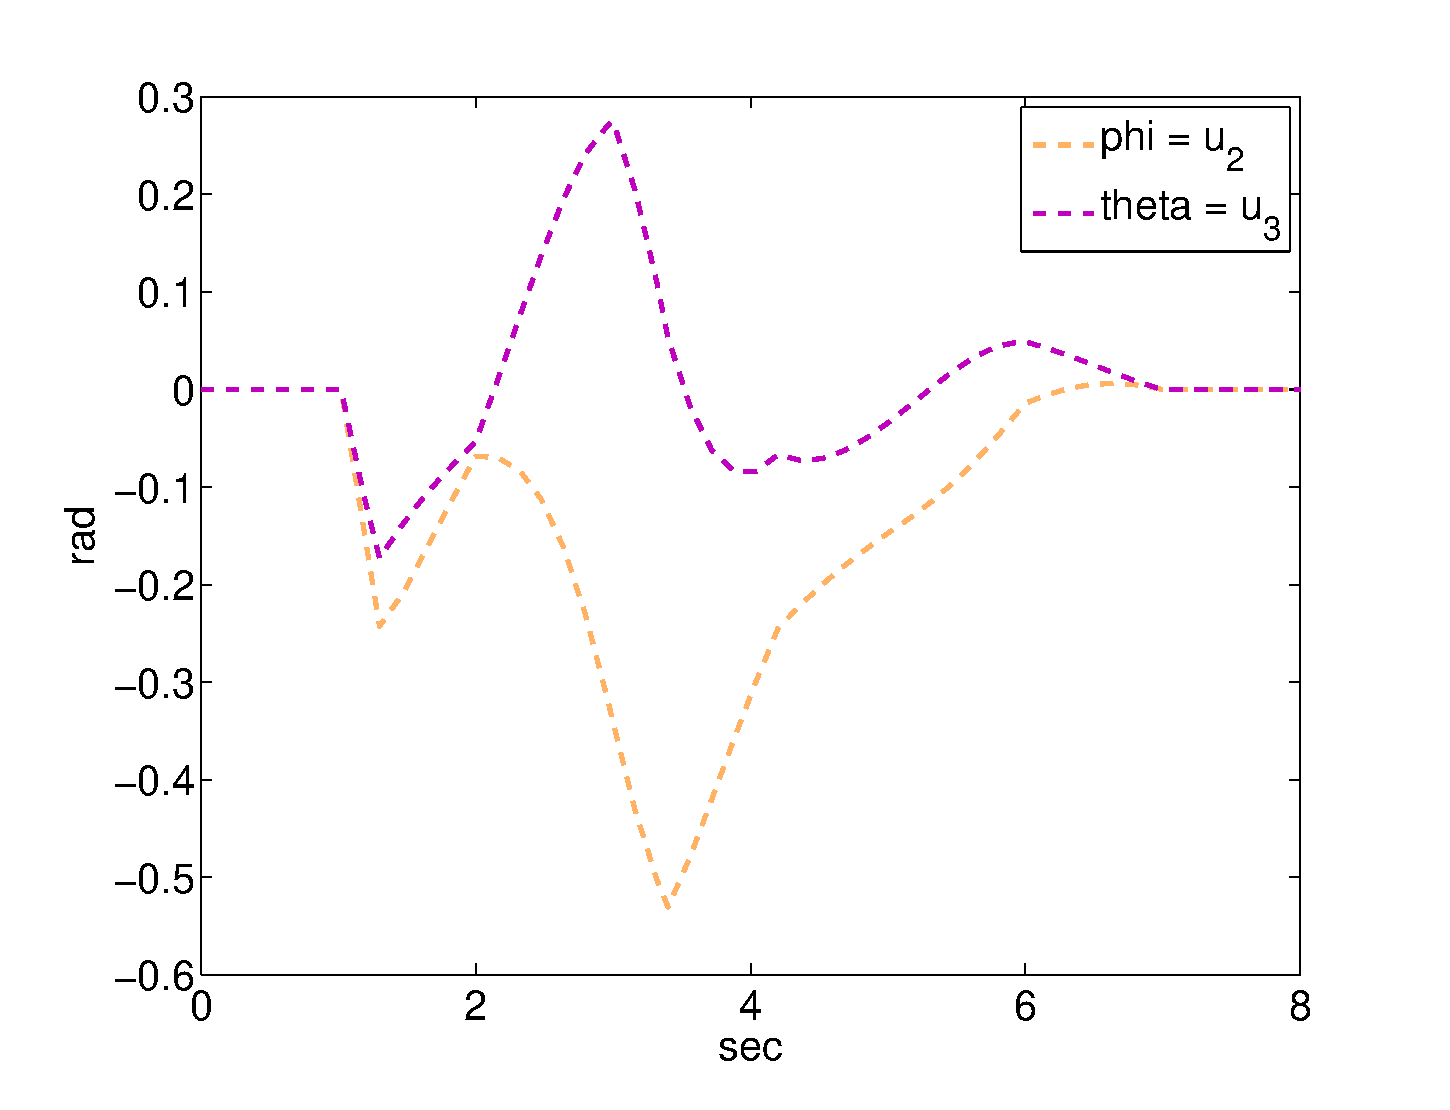
\includegraphics[width=0.5\textwidth]{images/inv_phitheta}
 			\label{fig:inv_phitheta}
 		}
 			\subfloat[Beschleunigungswerte im Translationsmodell]{
 				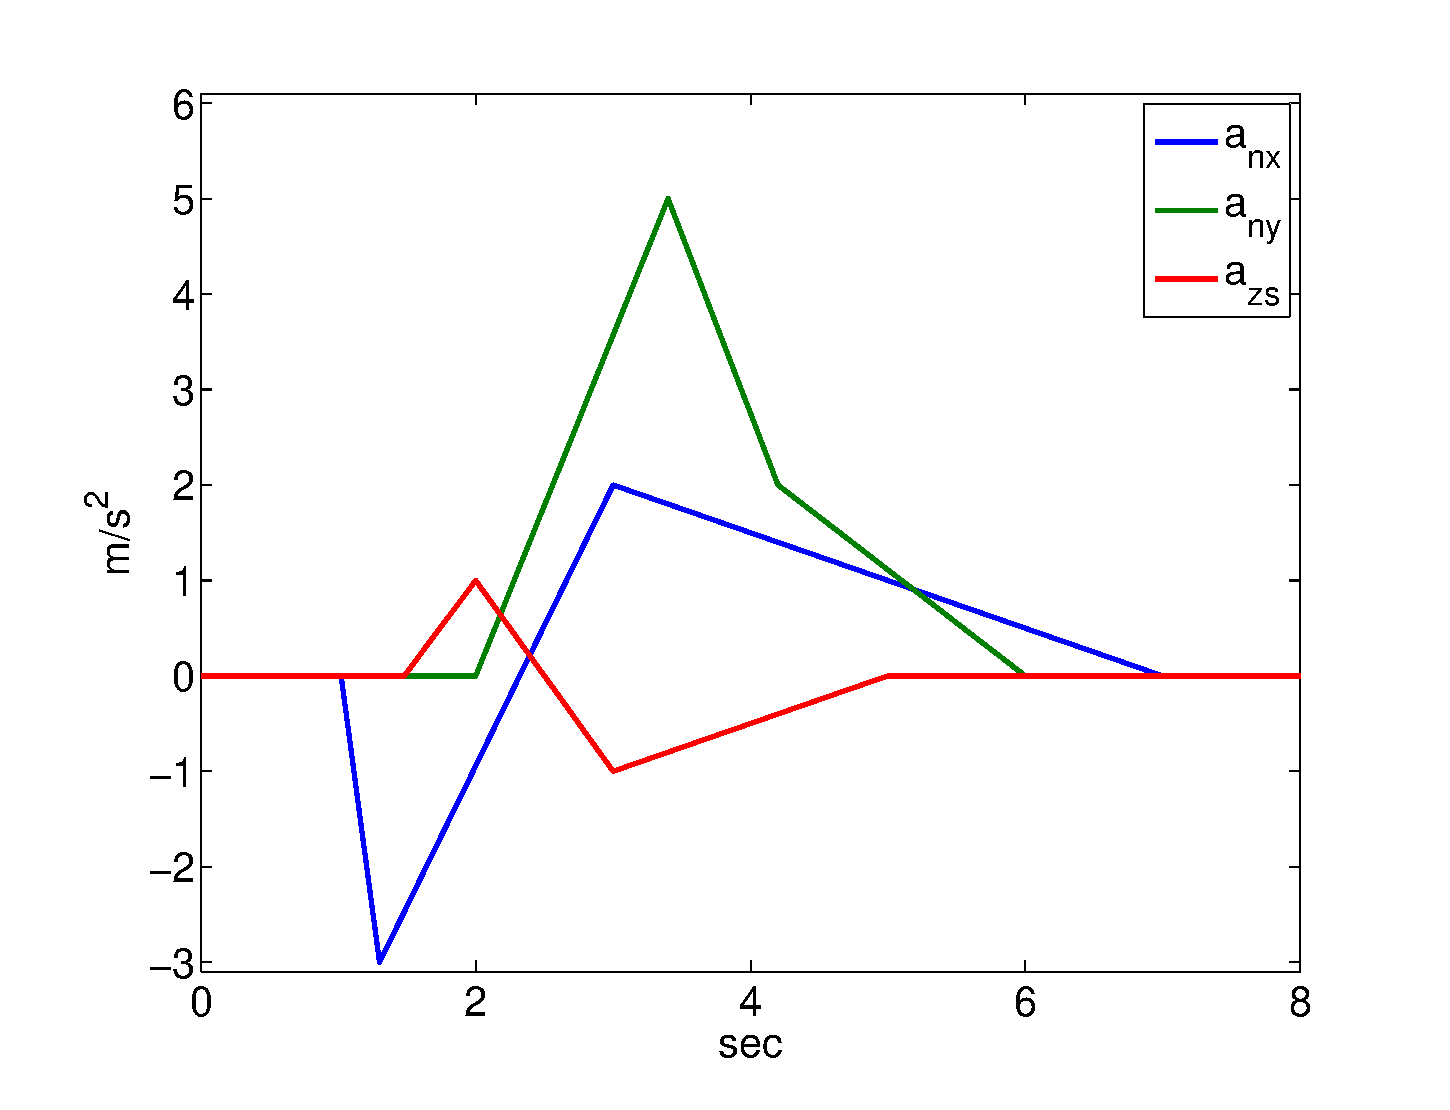
\includegraphics[width=0.5\textwidth]{images/inv_amdl}
 				\label{fig:inv_amdl}
 			}
 	}	
 	\caption[Simulation Inversion]{Simulation der Inversion}
 	\label{fig:sim_inversion}
 \end{figure}



\section{Vorsteuerung/Referenzmodell}
\label{sec:referenzmodell}
Eine Vorsteuerung erzeugt anhand einer Sollwertvorgabe einen Stellgr��enverlauf, der ben�tigt wird um System im st�rungsfreien Fall in diesen Zustand zu �berf�hren. In \cite{Achtelik11} wird deshalb auch von Referenzmodell gesprochen. 
 
Im Sachen Positionsregelung bedeutet dies, es wird eine anzufliegende Position $ P^n_{cmd} $ �bergeben. Daraus generiert die Vorsteuerung eine Trajektorie. Der Pfad $ P^n_{ref} $ mit dem der Quadrocopter in den Zustand �berf�hrt werden soll muss dabei einmal stetig differenzierbar sein. Der Grund, die Stellgr��e der Inversion sind Beschleunigungsvorgaben. Demzufolge muss die zweite Ableitung der Position mindestens st�ckweise existiert. Damit dies gew�hrleistet ist, ist nach \cite{deutNL} folgende Differenzialgleichung f�r das Referenzmodell aufzustellen. 
%Zur Vorgabe des gew�nschte ben�tigt man als Vorsteuerung ein Referenzmodell. Diesem werden die anzufliegenden Positionen $ P^n_{cmd} $ �bergeben. Aufgabe der Vorsteuerung ist es daraus eine Trajektorie zu generieren. Diese beschreibt den Pfad �ber den der Quadrocopter in diese Koordinate �berf�hrt wird. Da die neuen Eingangsgr��en $ u_f $ des zustandslinearisierten Modells Beschleunigungsvorgaben sind, muss der Verlauf der Positionsvorgabe der Vorsteuerung $ P^n_{ref} $ einmal stetig differenzierbar sein, sodass die zweite Ableitung existiert. Damit dies gew�hrleistet kann nach \cite{deutNL} die E/A Dynamik f�r dieses System �ber folgende Formel vorgegeben werden.
\begin{equation}
	\ddot{P}^n_{ref} + c_1 \cdot \dot{P}^n_{ref}+c_0\cdot P^n_{ref}=c_0 \cdot P^n_{cmd}
	\label{eq:dynref}
\end{equation}
Hierbei kann die Dynamik mit der das Flugger�t �berf�hrt werden soll, �ber die Koeffizienten eingestellt werden. Stellt man f�r (\ref{eq:dynref}) die �bertragungsfunktion $ G(s) $ auf.
\begin{equation}
\begin{split}
G(s)=\frac{P^n_{cmd}}{P^n_{ref}} &=\frac{c_0}{s^2+c_1\cdot s+c_0}\\
&= \frac{1}{\frac{1}{c_o}s^2+\frac{c_1}{c_0}\cdot s+1}
\end{split}	
\label{eq:gsref}
\end{equation}
Kann man erkennen das diese in ihrer Form einem PT2-Glied entspricht.
\begin{equation}
	G_{PT2}(s)=\frac{1}{(\frac{1}{\omega_o})^2s^2+\frac{2D}{\omega_0}\cdot s+1}
	\label{eq:gspt2}
\end{equation}

Setzt man (\ref{eq:gspt2}) mit (\ref{eq:gsref}) gleich kann man die Koeffizienten $ c_0 $ und $ c_1 $ abh�ngig der gew�nschten Eigenfrequenz $ \omega_0 $ und D�mpfung $ D $ w�hlen.
\begin{equation}
c_0= \omega_0^2
\label{eq:ref_c0}
\end{equation}
\begin{equation}
c_1= 2 D\omega_0
\label{eq:ref_c1}
\end{equation}
Der Vorteil, die Dynamik der Vorsteuerung ist �ber die in den Grundlagen der Regelungstechnik vermittelten Entwurfskriterien f�r PT2-Glieder einstellbar.
So l�sst sich �ber $ \omega $ einstellen wir schnell die Zielkoordinate erreicht werden soll. Das wie, l�sst sich �ber die D�mpfung $ D $ bestimmen. So wird f�r alle $ D \le 1 $ eine Pfad ohne �berschwinger generiert. 
Die Dynamikvorgabe ist jedoch durch die maximal zul�ssige Stellgr��e beschr�nkt. So kann zumindest $ \omega $ nicht beliebig Gro� gew�hlt werden. 

Der Stellgr��enverlauf $ u_{f_{ref}} = \ddot{P}^n_{ref}  $ ist somit �ber (\ref{eq:dynref}) mit (\ref{eq:ref_c0}) und (\ref{eq:ref_c1}) folgenderma�en festgelegt.
\begin{equation}
u_{f_{ref}} = \omega_0^2 \cdot(P^n_{cmd}-P^n_{ref})-2D\omega_0\cdot \dot{P}^n_{ref}
\label{eq:ref_mdl}
\end{equation}
%Vorteil dieser Darstellung ist, das die Dynamik der Vorsteuerung �ber die in den Grundlagen der Regelungstechnik \cite{lunze08} vermittelten Entwurfskriterien f�r PT2-Glieder bestimmen l�sst. So ist die Schwingungsf�higkeit �ber die D�mpfung $ D $ beeinflussbar ($ D \le 1 $, keine Schwingung). Mit $ \omega_0 $ kann schlie�lich eingestellt werden wie schnell die Zielkoordinaten erreicht werden sollen. $ \omega $ ist da bei durch die maximal zul�ssige Stellgr��e beschr�nkt.
\begin{figure}
	\centering
	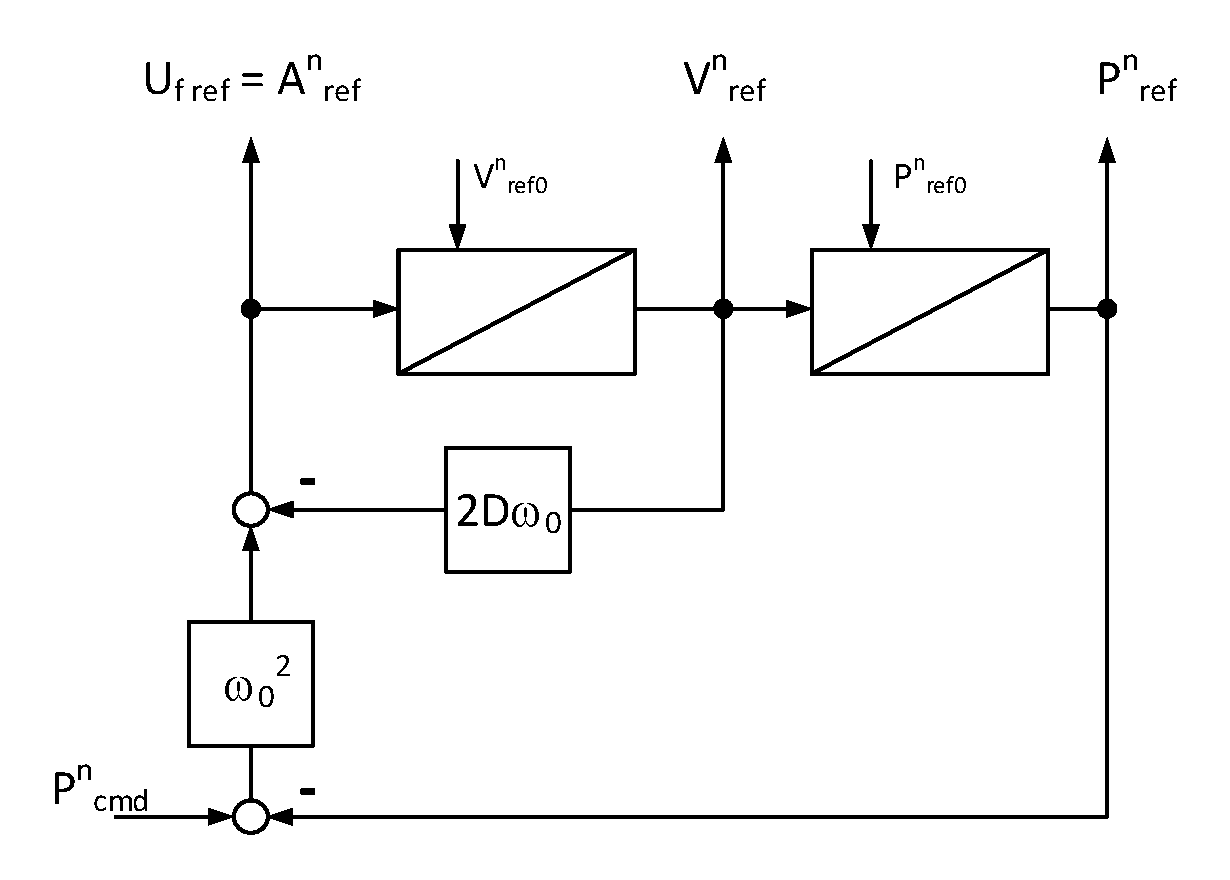
\includegraphics[width = \textwidth]{images/refmdl}
	\caption[]{Strukturbild Vorsteuerung} %
	\label{fig:strucref}
\end{figure}
Das resultierende Strukturbild der Vorsteuerung ist in Abbildung \ref{fig:strucref} visualisiert. F�r ein Positionsverschiebung von $ 1~m $ erzeugt das Referenzmodell die in Abbildung \ref{fig:tragen} Trajektorie bzw. den in Grafik \ref{fig:tragen_aref} dargestellten Stellwertverlauf. Hier ist anzumerken, das  aufgrund der entkoppelten Integriererketten (Kapitel \ref{sec:exkt.zstdlin}) eine separate Dynamikvorgabe f�r jeden Zweig des zustandslinearisierten Modells m�glich ist. 
 \begin{figure}
 	\centering{
 		\subfloat[Positionsvorgabe �ber $ p_{cmd} $ und generierte Positionsvorgabe $ p_{ref} $]{
 			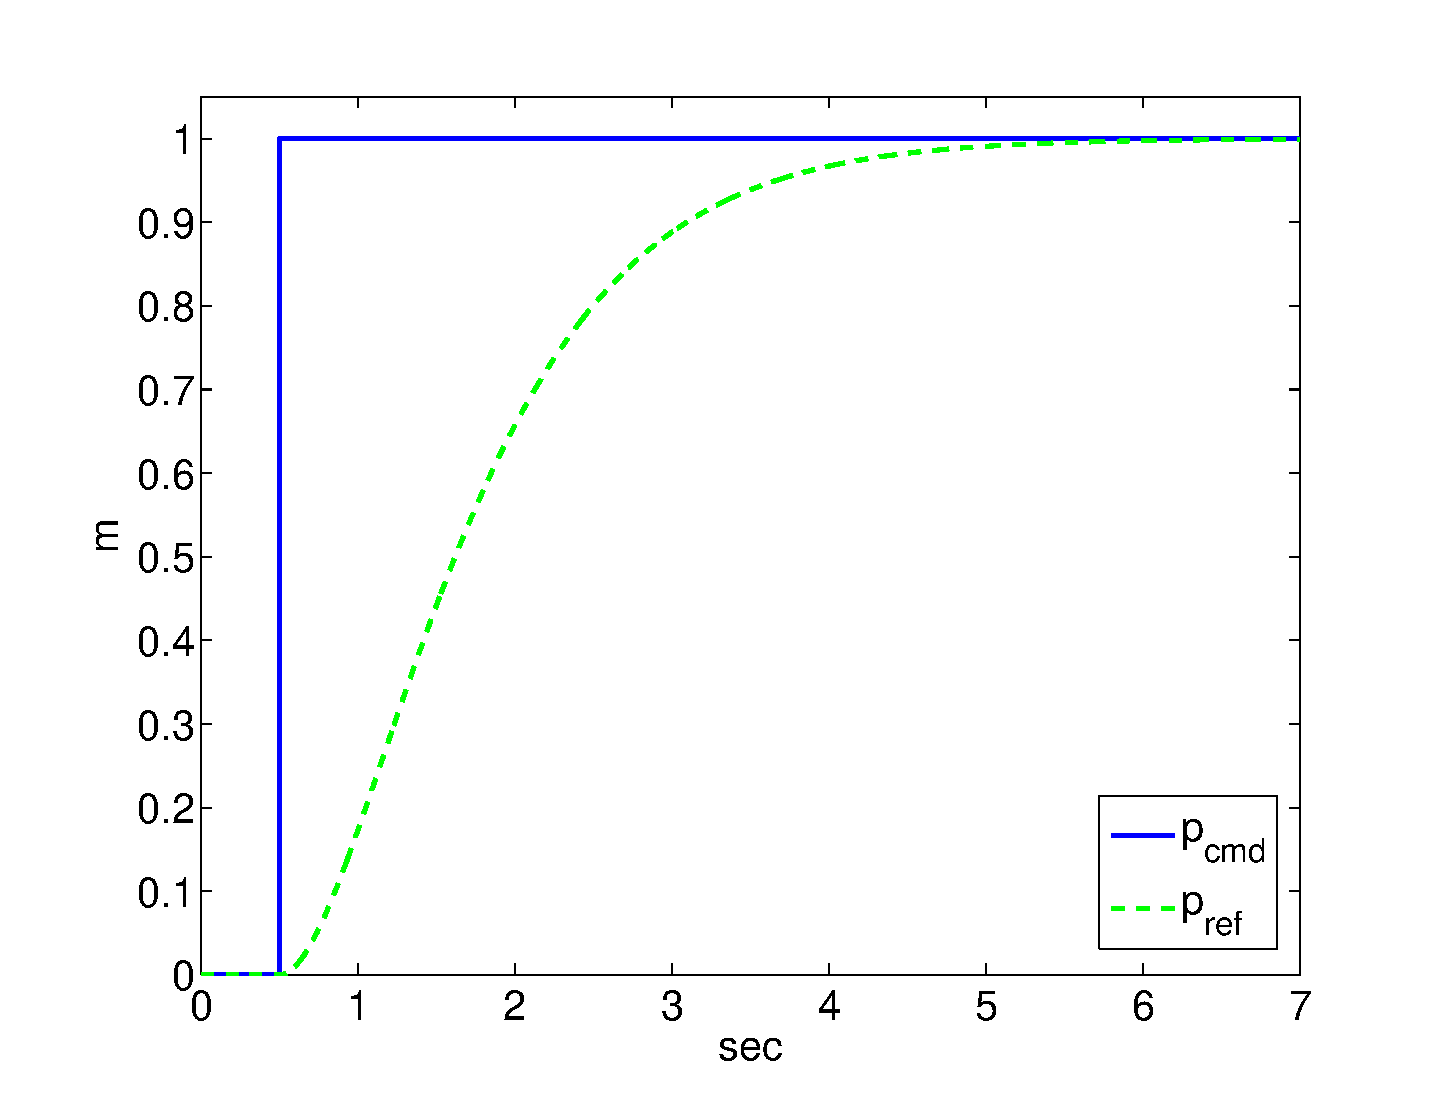
\includegraphics[width=0.5\textwidth]{images/p_cmdref}
 			\label{fig:tragen_pcmdref}
 		}\\
 		\subfloat[Geschwindigkeitsvorgabe $ v_{ref} = \dot{p}_{ref} $ der Trajektorie]{
 			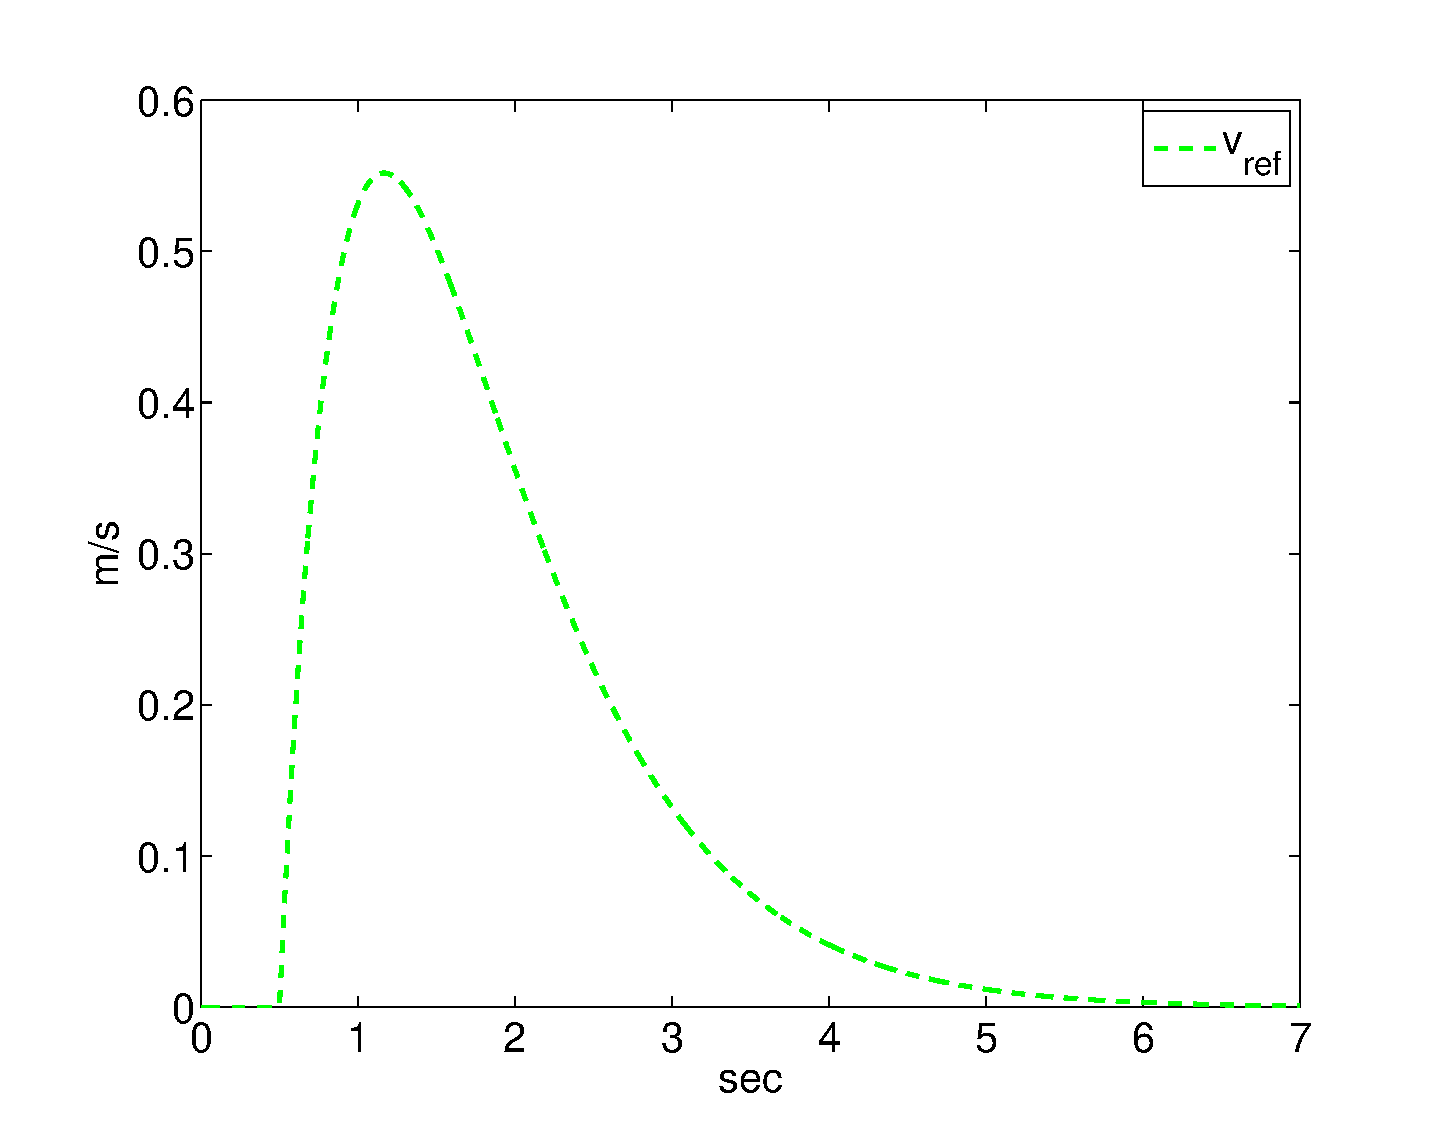
\includegraphics[width=0.5\textwidth]{images/v_ref}
 			\label{fig:tragen_vref}
 		}
 		\subfloat[Beschleunigungsvorgabe $ u_{f_{ref}} = a_{ref} = \ddot{p}_{ref}$]{
 			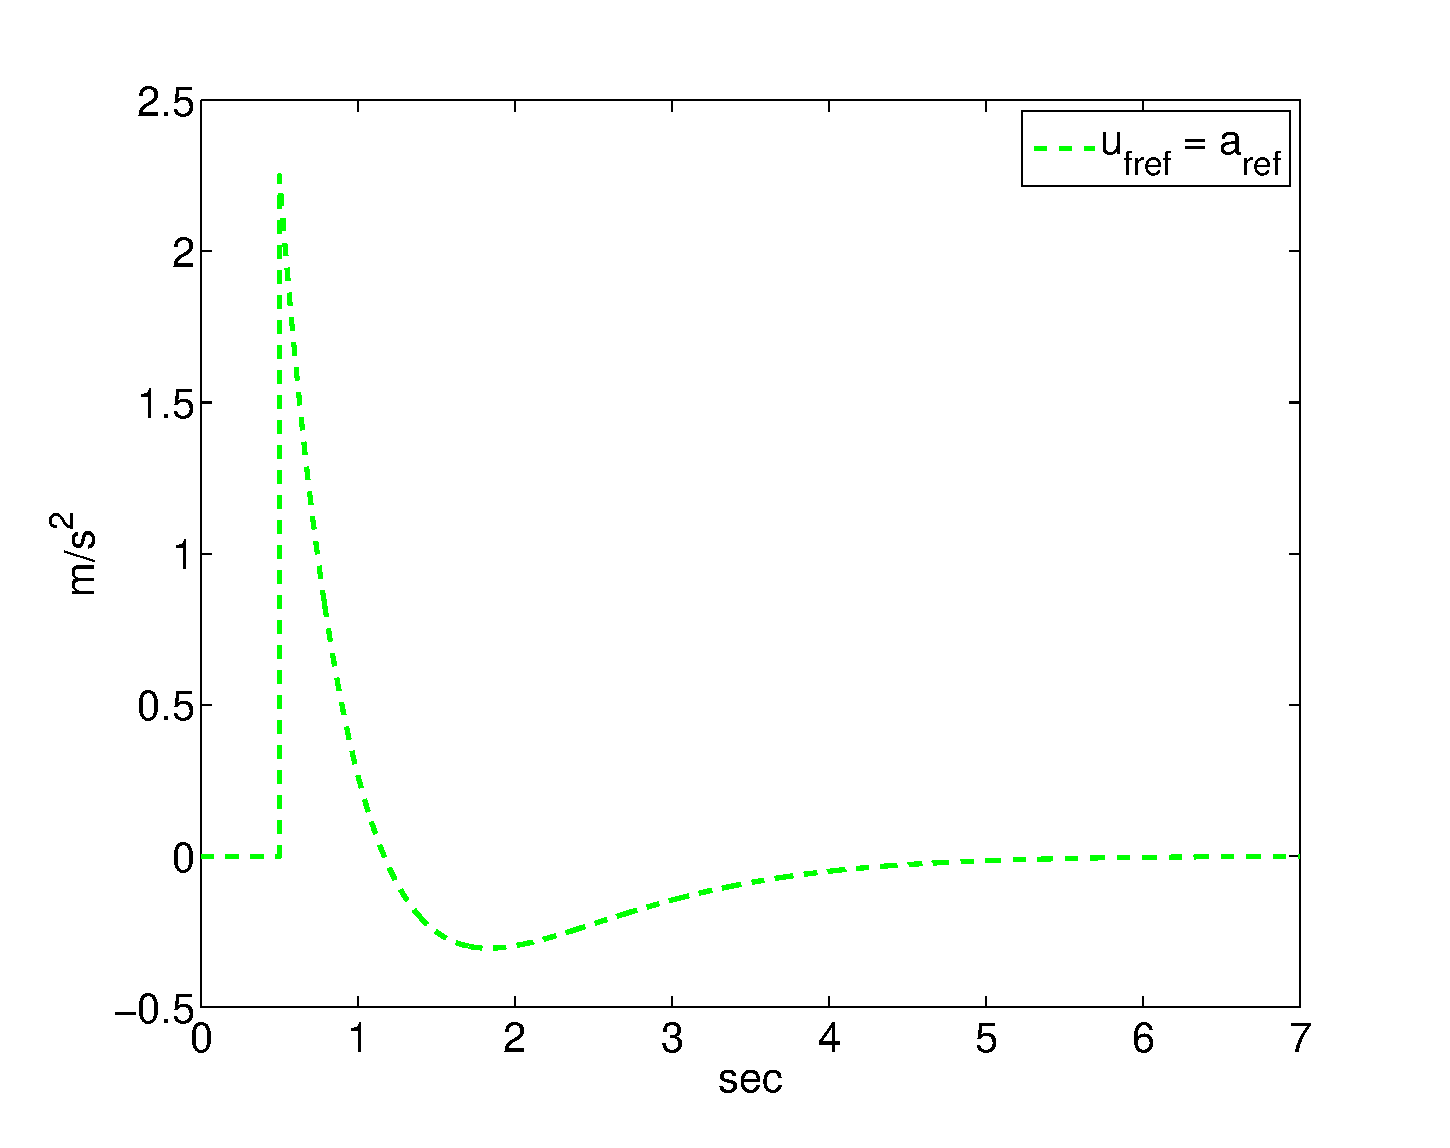
\includegraphics[width=0.5\textwidth]{images/a_ref}
 			\label{fig:tragen_aref}
 		}
 	}	
 	\caption[Simulationsergebnisse Referenzmodell]{Simulationsergebnis des Referenzmodells f�r eine Achse mit $ \omega_0 = 1.5~Hz$ $ D = 1 $}
\label{fig:tragen}
 \end{figure}
Weiterhin besteht die M�glichkeit die Vorsteuerung auszubauen, so dass  Geschwindigkeitsvorgaben gemacht werden k�nnen. Dies erleichtert unter anderem das manuelle Navigieren mittels einer Fernsteuerung. Dabei erfolgt die Vorgabe der Soll-Geschwindigkeiten $ v^o_{cmd} $ im o-frame. Diese Vorgabe wird ins n-frame transformiert und dort �ber die Zeit integriert. Somit ergibt sich eine stetig Positionsvorgabe f�r $ P^n_{cmd} $. 

\begin{equation}
P^n_{cmd} = \int (M_z^T\cdot v^o_{cmd}) dt + P^n_{cmd_0}
\label{eq:v_Pcmd}
\end{equation}

Mit dieser wird das Referenzmodell (\ref{eq:ref_mdl}) gespie�t. Es wird ein Stellgr��e erzeugt f�r das die Position des Quadrocopter der stetigen Positionsvorgabe (\ref{eq:v_Pcmd}) folgt. Die maximale Geschwindigkeit ist deshalb durch die Grenzfrequenz $ \omega_0 $ des Referenzmodells begrenzt. Je gr��er $ \omega_0 $ die desto h�her die m�gliche Geschwindigkeit.
  
Die Vorsteuerung ist somit f�r alle Anwendungszwecke entworfen. Speist man das exakt Zustandslinearisierte mit dem in Abbildung \ref{fig:tragen} generierten Sollwertverlauf so folgt der Quadrocopter der Trajektorie. Dies gilt allerdings nur f�r den Fall konsistenter Anfangszust�nde (Abbildung \ref{fig:vor_ohnestr}). Ist dies nicht gegeben, ist wie in Abbildung zu erkennen das Positionsverlauf des Translationsmodell f�r den gleichen Stellgr��enverlauf nicht der Referenz entspricht. Das gleiche gilt f�r Unsicherheiten der Modellparameter (Abbildung \ref{fig:vor_unsichmdlpara}). Hierbei berechnet die Inversion einen unzureichenden oder �berdimensionierten Schubvektor. 
%Simuliert man das Modell (Abbildung \ref{fig:Gesamtinversion}) inklusive des Stellgesetzes der Vorsteuerung Gleichung (\ref{eq:ref_mdl}) f�r konsistente Anfangsbedingungen $ P_{ref0}^n = P_0^n $ so ergibt sich die gew�nschte Flugkurve. In der Realit�t ist die Konsistens der Angfangsbedingungen jedoch nicht immer gegeben. 
Au�erdem k�nnen �u�ere Krafteinwirkungen wie zum Bespiel Winde wirken, die den Quadrocopter von der Trajektorie auslenken. Um all diesen Effekten entgegenzuwirken ben�tigt man einen Folgeregler. Dessen Aufgabe besteht darin diese Einfl�sse zu eliminieren, sodass das Modellverlauf auch im gest�rten Fall der Trajektorie entspricht.
 \begin{figure}
 	\centering{
 		\subfloat[Konsistente Anfangszust�nde $ p_{ref_0}~=~p_{mdl_0}~=~0 $ und $ v_{ref_0}~=v_{mdl_0}~=~0 $, ideales Modell]{
 			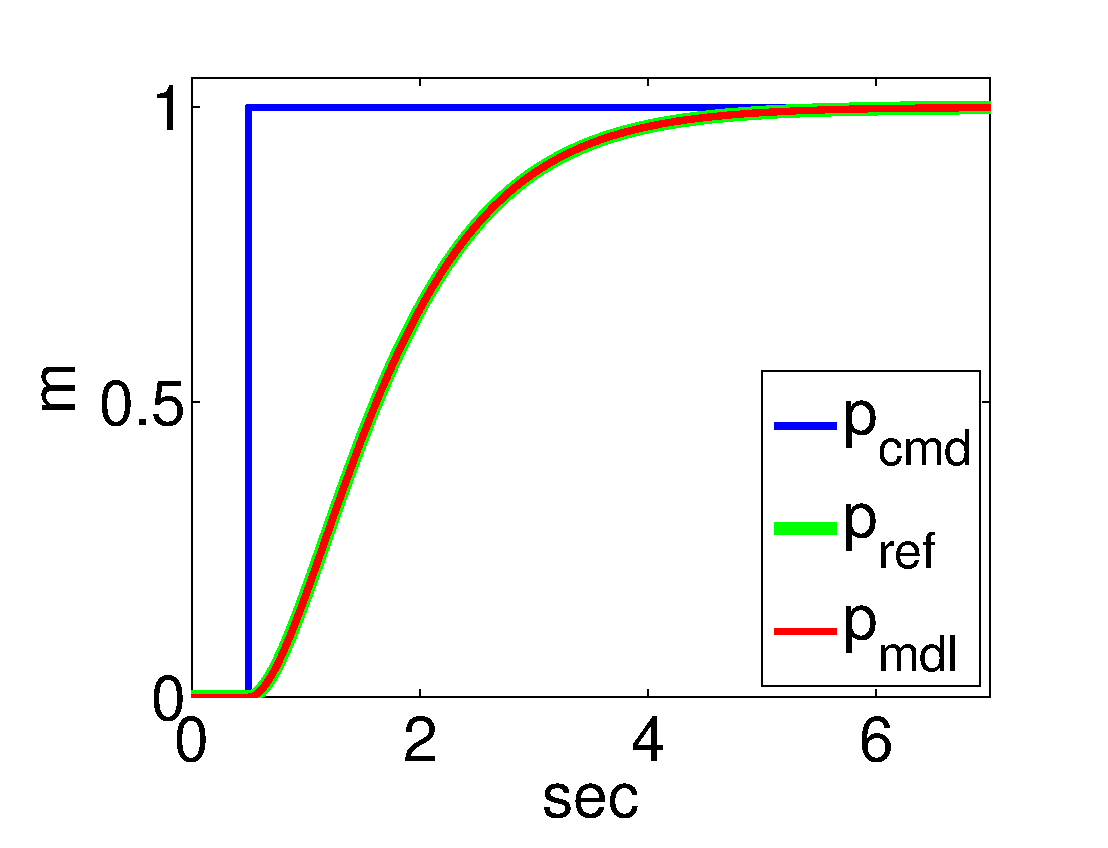
\includegraphics[width=0.5\textwidth]{images/vstr_ohnest}
 			\label{fig:vor_ohnestr}
 		}\\
 		\subfloat[Inkonsistene Anfangszust�nde $ p_{ref_0}~=~0~\ne~p_{mdl_0}~=~0.3 $ und $ v_{ref_0}~=~0~\ne~v_{mdl_0}~=~0.2 $, ideales Modell]{
 			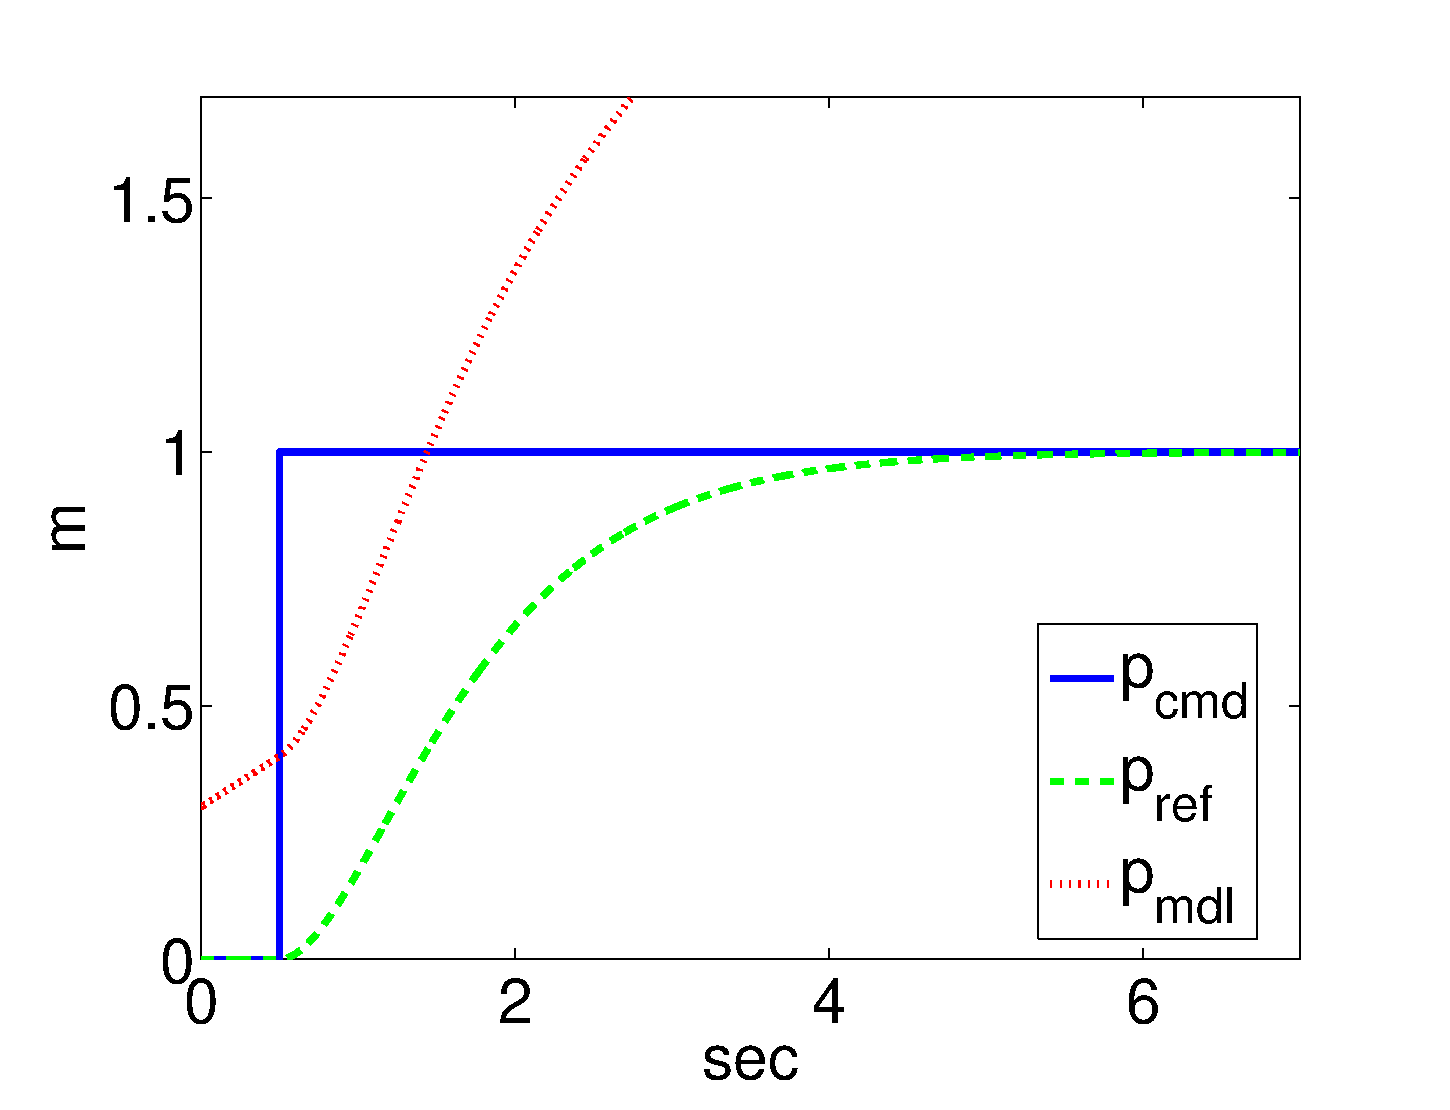
\includegraphics[width=0.5\textwidth]{images/p_p0_03_v0_02}
 			\label{fig:vor_inkonAzust}
 		}
 		\subfloat[Unsicherheit der Modellparamter $ m_{inv}~\ne~m_{mdl} $]{
 			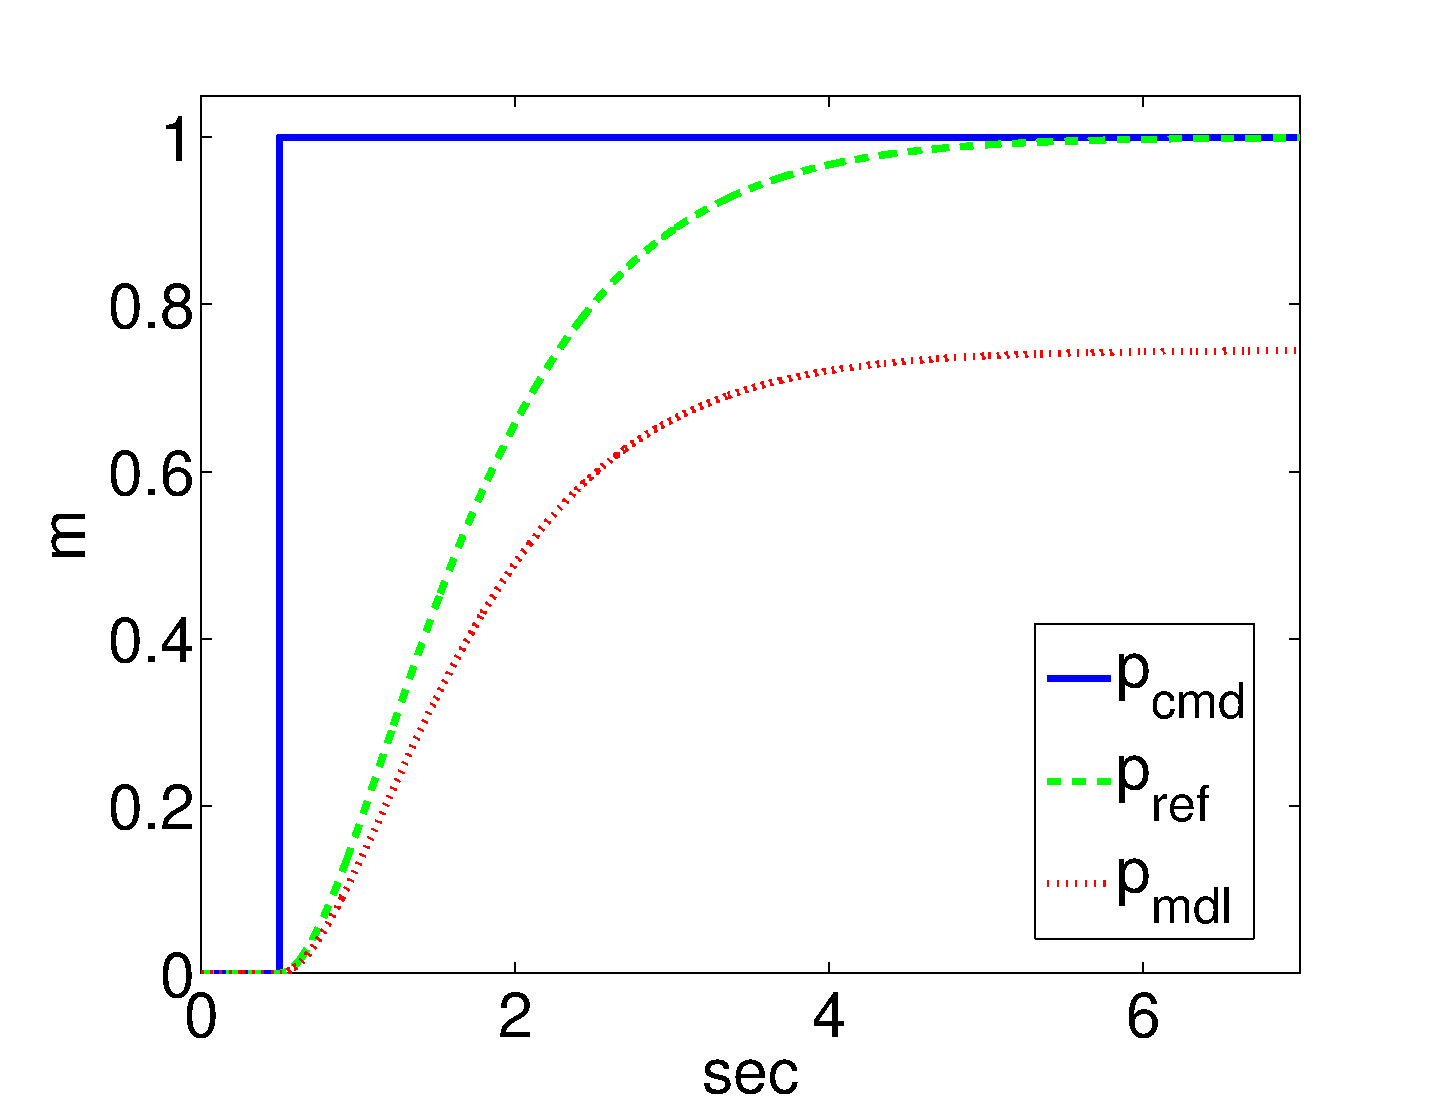
\includegraphics[width=0.5\textwidth]{images/p_m_mdl_2_5}
 			\label{fig:vor_unsichmdlpara}
 		}
 	}	
 	\caption[Referenzmodell als Vorsteuerung]{Steuerung der Regelstrecke �ber das Referenzmodell}
 	\label{fig:RefaliasVor}
\end{figure}
%++++++++++++++++++++++++++++++++++++++++++++++++++++++++++++++++++++++++++++++++++++++++++++++++++++++++
\section{Folgeregler}
\label{sec:folgeregeler}
Inkonsistente Anfangsbedingungen, externe St�rungen sowie Modellunsicherheiten bewirken einen Ausgangsfolgefehler $e = P^n_{ref} - P^n $. Dieser Pflanzt sich weiter fort, da es sich bei dem Stellsignal $  u_{f_{ref}} $ (\ref{eq:ref_mdl}) nicht um das Stellsignal $ u_f $ handelt welches den Quadrocopter zur�ck auf die Trajektorie f�hrt. Dies gilt auch im Falle eines unzureichenden Stellsignalverlaufs in Folge von Modellunsicherheiten. Modellieren l�sst sich die Fortpflanzung des Folgefehlers aufgrund des linearisierten Modells in Form einer doppelten Integriererkette. 
%Dieser ergibt sich durch die Fortpflanzung des f�r das reale System nicht ausreichenden Stellsignals $\ddot{e} = u_{f_{ref}} - u_f$. Das bedeutet, die Fehlerdynamik kann ebenfalls �ber eine zweifache Integriererkette modelliert werden. 
Zweifache Integriererkette ergo instabiles System. Damit sp�ter die Flugbahn des Quadrocopter mit der Solltrajektorie konvergiert, muss die Fehlerdynamik stabilisiert werden. 
%Daf�r ist es von n�ten, die Dynamik der Folgefehler vorgeben zu k�nnen. 
Zu diesem Zwecke werden die Zustandsgr��en des Ausgangsfolgefehlermodells zur�ckgef�hrt (Abbildung \ref{fig:r�ckfolgefeh}). Daraus ergibt sich f�r die Vorgabe, dass der Folgefehler $ e $ in einer endlichen Zeit gegen $ 0 $ strebt, folgende Differentialgleichung.
\begin{figure}
	\centering
	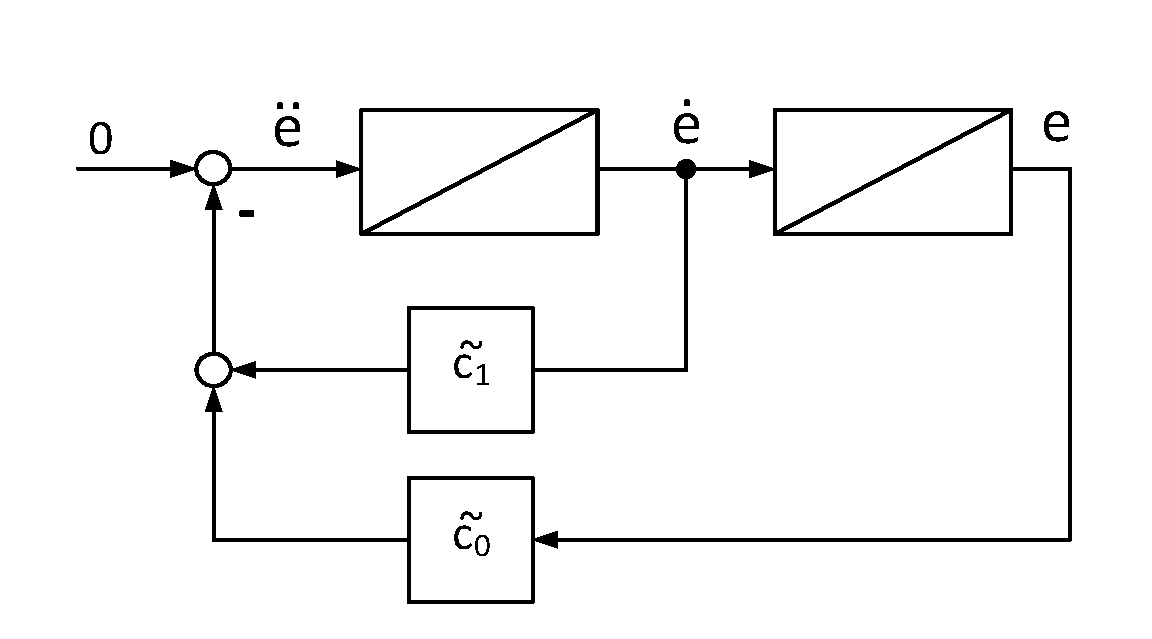
\includegraphics[width = \textwidth]{images/fehlermdl}
	\caption[]{Ausgabgsfolgefehlermodell mit Zustandsr�ckf�hrung} %
	\label{fig:r�ckfolgefeh}
\end{figure}
\begin{equation}
\ddot{e} + \tilde{c}_1 \cdot \dot{e}+ \tilde{c}_0\cdot e = 0
\label{eq:fehlerdyn}
\end{equation}
 mit 
\begin{equation}
\begin{split}
e &= P^n_{ref} - P^n\\
\dot{e} &= \dot{P}^n_{ref}-\dot{P}^n\\
\ddot{e} &= u_{f_{ref}} - u_f
\end{split}
\end{equation}
Diese kann nach $ u_f $ um gestellt werden. Damit ergibt sich das nachfolgende Stellgesetz f�r die Eingangsgr��e $ u_f $ des zustandslinearsierenten Systems welches den Folgefehler ausregelt. 
\begin{equation}
u_f = \underset{Vorsteuerung}{u_{f_{ref}}}+ \underset{Folgeregler}{\tilde{c}_1 \cdot (\dot{P}^n_{ref}-\dot{P}^n) +\tilde{c}_0\cdot (P^n_{ref} - P^n)}
\end{equation}
Die Ann�herungsverhalten ist Abh�ngig von den Koeffizienten $ \tilde{c}_0 $ und $ \tilde{c}_1 $. Anhand von \ref{eq:fehlerdyn} lassen sich f�r diese mittels der Polvorgabe (Kapitel \ref{subsec:polvor}) die Dynamik vorgegeben.

Nicht bek�mpft werden durch dieses Stellgesetz konstante Dauerst�rungen. Hervorgerufen zum Beispiel durch Winde die �ber einen l�ngeren Zeitraum als Konstant anzusehen sind. Mit einer konstanten Kraft wirken diese auf das Flugsystem. Beachtet man die von dieser Kraft hervorgerufenen Beschleunigungsbeitrag $ a_st $ in der Fehlerdifferenzialgleichung. 
\begin{equation}
\ddot{e} + \tilde{c}_1 \cdot \dot{e}+ \tilde{c}_0\cdot e +a_{st}= 0
\label{eq:fehlerdyn_st}
\end{equation}
Folgt im station�ren Zustand, das hei�t alle Zeitableitungen gleich Null, ein dauerhafter Positionsfehler.
\begin{equation}
e = -\frac{a_{st}}{\tilde{c}_0}
\end{equation} 
L�sung dieses Problems ist nach \cite{deutNL} die Erweiterung des Folgeregler mit einer Integrierenden Komponente.
\begin{equation}
\ddot{e} + \tilde{c}_1 \cdot \dot{e}+ \tilde{c}_0\cdot e + \underset{I-Anteil}{\tilde{c}_{-1} \int e(\tau)d\tau} +a_{st}= 0
\label{eq:integodif}
\end{equation} 
Der I-Anteil liefert einen Signalanteil zur Kompensation der St�rung im station�ren Zustand. Den Beweis daf�r erh�lt man, wenn man die Integro-Differentialgleichung (\ref{eq:integodif}) nach der Zeit ableitet. Danach ergibt sich Folgenden Differentialgleichung. 
\begin{equation}
	\dddot{e} + \tilde{c}_1 \cdot \ddot{e}+ \tilde{c}_0\cdot \dot{e} + \tilde{c}_{-1} \cdot e = 0
	\label{eq:ifehlerdyn}
\end{equation}
Im eingeschwungenen Zustand, ergibt sich so f�r den Positionsfehler
\begin{equation}
 e = 0
\end{equation}
Das Stellgesetz f�r einen Regler mit I-Anteil l�sst sich unter Vernachl�ssigung der Dauerst�rung $ a_{st} $ aus Gleichung (\ref{eq:integodif}) entwickeln (vgl. Abbildung \ref{fig:folgeregler}).
\begin{equation}
u_f = \underset{Vorsteuerung}{u_{f_{ref}}}+ \underset{Folgeregler\ inklusive\ I-Anteil}{\tilde{c}_1 \cdot (\dot{P}^n_{ref}-\dot{P}^n) +\tilde{c}_0\cdot (P^n_{ref} - P^n)+\tilde{c}_{-1} \int e(\tau)d\tau}
\end{equation}
\begin{figure}
	\centering
	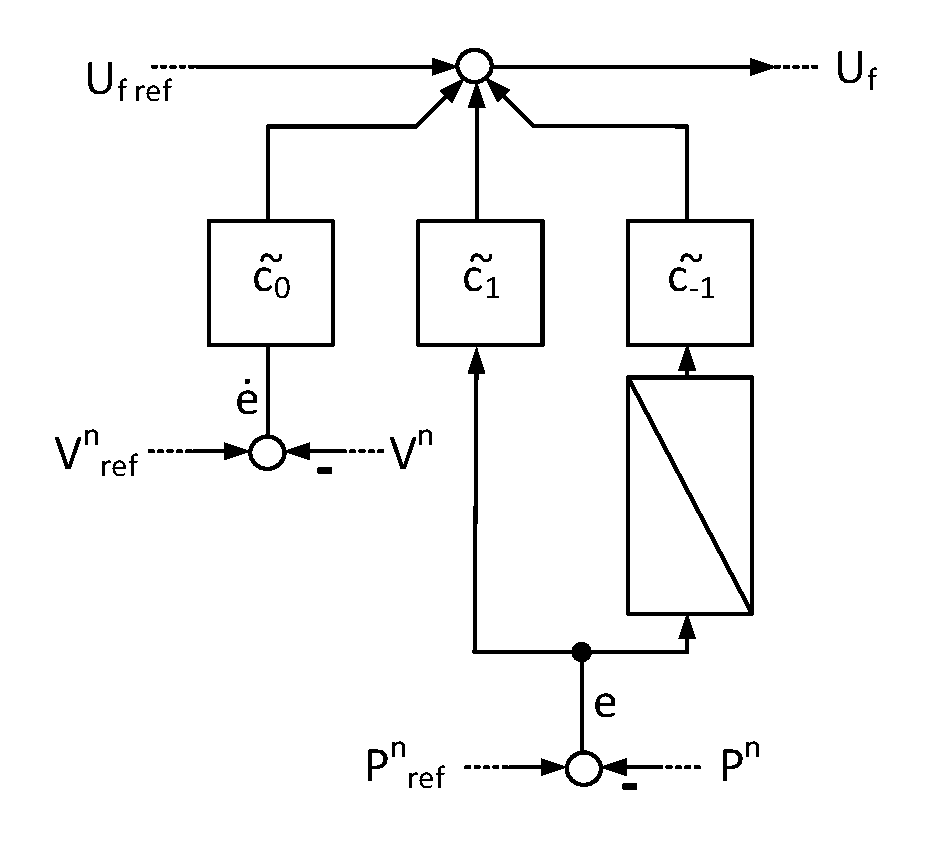
\includegraphics[width = 0.75\textwidth]{images/folgreg}
	\caption[Folgeregler]{Folgeregler} %
	\label{fig:folgeregler}
\end{figure}
Dieses Stellgesetz f�hrt den Quadrocopter entlang Referenztrajektorie. Zur erkennen ist dies auch in der Simulation (\ref{fig:folg_RefaliasVor}) mit Regler Regler. So wird f�r Inkonsistene Anfangsbedingungen (Abbildung \ref{fig:folg_inkonAzust}) das Flugger�t auf die Trajektorie gef�hrt. F�r Modellunsicherheiten (Abbildung \ref{fig:folg_unsichmdlpara}) passt der Folgeregler das Stellsignal so an, das der Quadrocopter entlang des vorgegebenen Pfad fliegt. Vergleich hierzu reine Vorsteuerung (Abbildung \ref{fig:RefaliasVor}).

Wie auch schon zuvor kann das Einschwingverhalten f�r den Folgeregler mit I-Anteil �ber die Polvorgabe festgelegt werden. F�r diesen ist die Differentialgleichung (\ref{eq:ifehlerdyn}) zu verwenden. 
 \begin{figure}
 	\centering{
 		
 		\subfloat[Inkonsistene Anfangszust�nde $ p_{ref_0}~=~0~\ne~p_{mdl_0}~=~0.3 $ und $ v_{ref_0}~=~0~\ne~v_{mdl_0}~=~0.2 $, ideales Modell]{
 			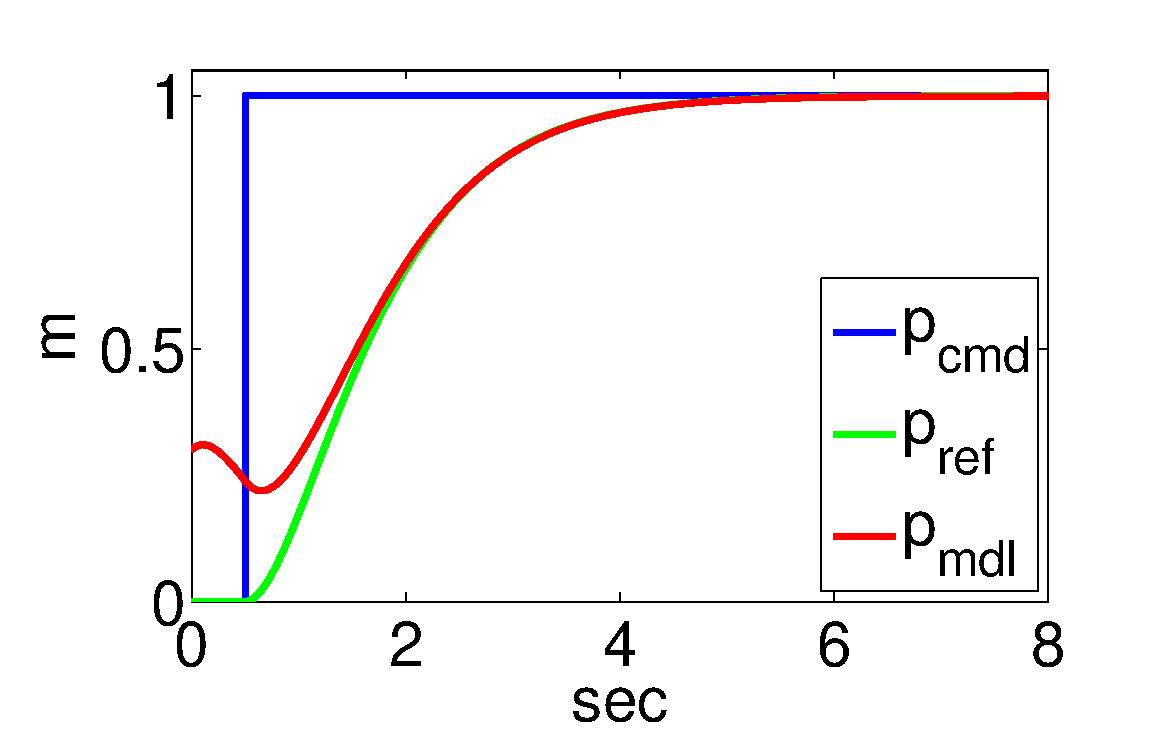
\includegraphics[width=0.5\textwidth]{images/p_p0_03_v0_02_Kd_4_Kp_5_Ki_001}
 			\label{fig:folg_inkonAzust}
 		}
 		\subfloat[Unsicherheit der Modellparamter $ m_{inv}=1.863~\ne~m_{mdl}=2.5 $]{
 			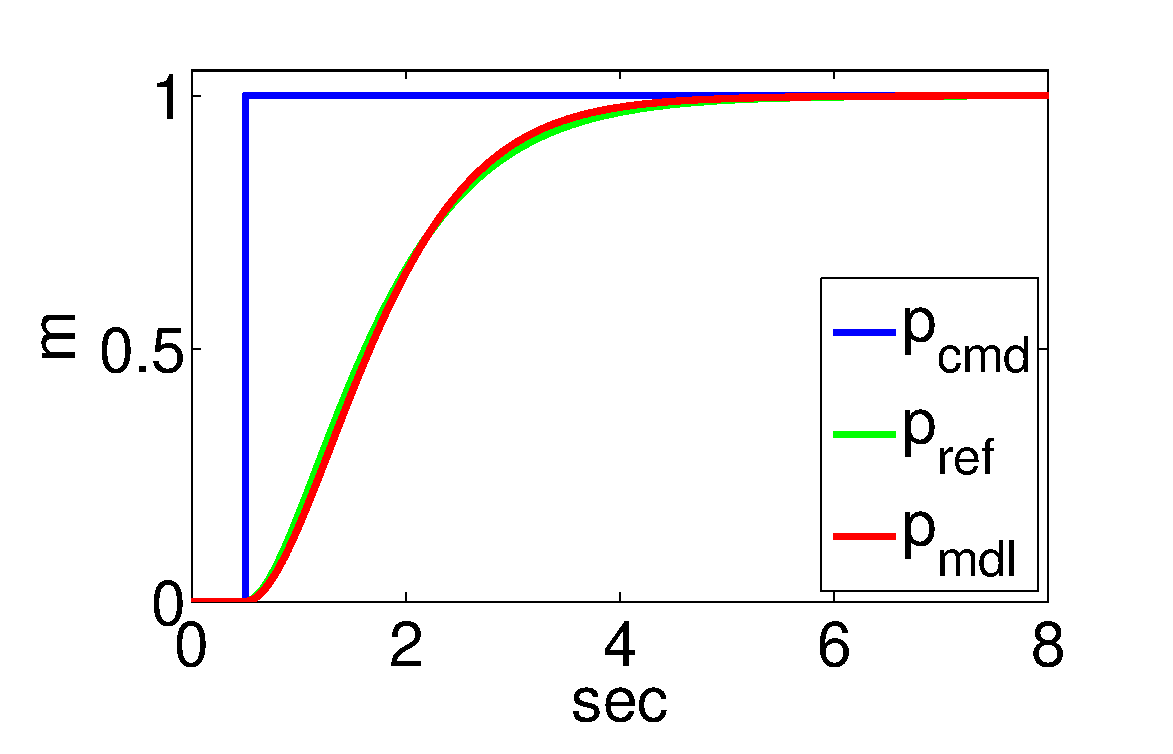
\includegraphics[width=0.5\textwidth]{images/p_m_mdl_2_5_Kd_4_Kp_5_Ki_001}
 			\label{fig:folg_unsichmdlpara}
 		}
 	}	
 	\caption[Grafiken Folgeregler]{Auswirkung von Folgeregler ($\tilde{c}_1=4$, $\tilde{c}_0=4$, $\tilde{c}_{-1}=0.01 $) auf inkonsistente Anfangszust�nde und Modellunsicherheiten }
 	\label{fig:folg_RefaliasVor}
 \end{figure}
 
 
 %++++++++++++++++++++++++++++++++++++++++++++++++++++++++++++++++++++++++++++++++++++++++++++++++++++++++++++++++++++
\subsection{Einstellung der Dynamik mittels Polvorgabe}
\label{subsec:polvor}
Anhand der Lage der Polstellen einer �bertragungsfunktion, k�nnen R�ckschl�sse �ber die Stabilit�t und das Einschwingverhalten getroffen werden. Ziel einer Zustandsregelung, wie der Folgereregelung, ist die Pollagen der zu regelnden Strecke so zu verschieben, dass das Einausgangsverhalten die gew�nschte Dynamik aufweist.

Zun�chst ist zu kl�ren was die Polstellenlage in der komplexen Ebene �ber das Verhalten aussagt. Dabei entspricht die Anzahl der Pole $ \lambda_i $ der Ordnung $ n $ des Systems.
\begin{figure}
	\centering
	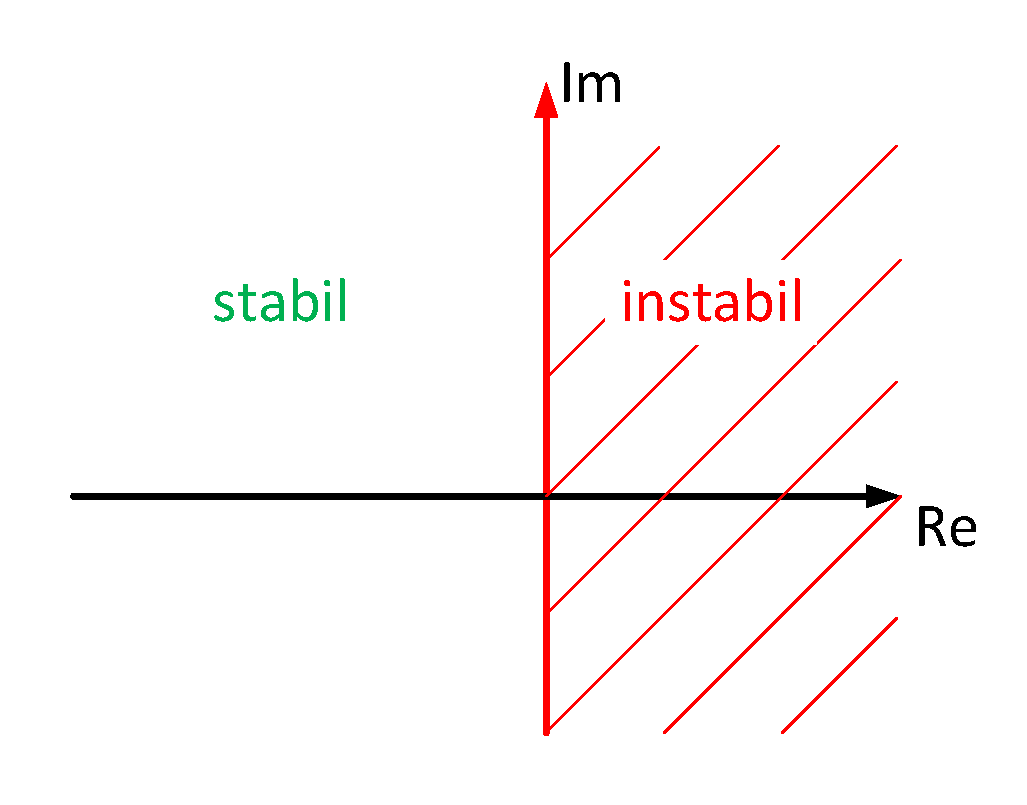
\includegraphics[width = 0.75 \textwidth]{images/stabgeb}
	\caption[Stabilit�tsgebiet]{Stabilit�tsgebiet} %
	\label{fig:stabgeb}
\end{figure}
\begin{itemize}
	\item Befinden sich alle Pole $ \lambda_i $ links der Imagin�rachse ($ Re(\lambda_i) < 0 $), so ist das System asymptotisch stabil, ansonsten instabil (Abbildung \ref{fig:stabgeb}).
	\item Komplexe Pole k�nnen nur in Formen von Polpaaren auftauchen. Ist ein Komplexes Polpaar vorhanden, f�hrt das System nach Anregung eine Schwingung aus . Befindet sich die Polpaare in der linken Halbebene des Imagin�rteil, nimmt die Amplitude der Schwingung exponentiell ab.
	\item Je weiter links sich die Pole auf der reellen Achse befinden, desto schneller ist das System. 
	\item Bei mehreren Polstellen wird das Verhalten haupts�chlich �ber den Pole bzw. die Polpaare mit dem gr��ten Realteil bestimmt. Sie werden deshalb als dominante Pole bezeichnet.
\end{itemize}
Betrachtet man eine beliebige �bertragungsfunktion im Bildbereich.
\begin{equation}
G_e(s) = \frac{Z(s)}{N(s)}
\label{eq:Ge}
\end{equation}  
Entsprechen die Polstellen $ \lambda_i $ des Systems, denn Nullstellen $ s_i $ des Nennerpolynom.
\begin{equation}
N(s)=  s^n+c_{n-1} \cdot s^{n-1}+ \cdots + c_1 \cdot s+ c_0 = \prod\limits_{n}^{i=1} (s-\lambda_i)= 0
\label{eq:N}
\end{equation}
Das dynamische Verhalten kann anhand dieser Pollage analysiert werden. Im Umkehrschluss k�nnen f�r frei w�hlbare Koeffizienten des Nennerpolynoms die Dynamik �ber Vorgabe von Polstellen $ \lambda_{si} $ erfolgen. Dies erfolgt �ber einen Koeffizientenvergleich.
\begin{equation}
N(s)=  s^n+c_{n-1} \cdot s^{n-1}+ \cdots + c_1 \cdot s+ c_0 =\prod\limits_{n}^{i=1} (s-\lambda_{si}) 
\end{equation}
Somit ist es m�glich �ber die Koeffizienten von (\ref{eq:fehlerdyn}) oder (\ref{eq:ifehlerdyn}) das Einschwingverhalten  des Folgereglers mittel der Platzierung von Polen vorzugeben. Wie jedoch die Polstellen optimal bestimmt, daf�r gibt es keine generelle Vorgehensweise. In der Regel werden sie empirisch �ber Simulationen festgelegt. Anschlie�end am realen Modell getestet und gegebenenfalls optimiert. Diese Optimierung gesieht meist h�ndisch. Allerdings gibt es hier Bem�hungen diese letzte Optimierung am realen System automatisiert durchzuf�hren. 
  
\subsection{Automatische Optimierung der Reglerparameter}
\label{sec:selftun}
In der Simulation ermittelte Parameter m�ssen meist f�r das realen System leicht angepasst werden. Von Vorteil ist es deshalb, einen Algorithmus zu implementieren, der online und kontinuierlich die Einstellung optimiert. Die Bezeichnung dieses Vorgangs hei�t selftuning. 

Da der implementierte Folgeregler inklusive I-Anteil besteht aus einem Proportionalverst�rker $ P $, einem Differentiellen Anteil $ D $ sowie einem Integrationsanteil $ I $ zusammensetzt.
\begin{equation}
u_f = \underset{Vorsteuerung}{u_{f_{ref}}}+ \underset{D-Anteil}{\tilde{c}_1 \cdot (\dot{P}^n_{ref}-\dot{P}^n)} +\underset{P-Anteil}{\tilde{c}_0\cdot (P^n_{ref} - P^n)}+\underset{I-Anteil}{\tilde{c}_{-1} \int e(\tau)d\tau}
\end{equation}
K�nnen Tuningalgorithmen angewandt werden, die f�r einen PID-Regler entwickelt worden sind. So kann der unter \cite{selftun} vorgestellte Algorithmus angewendet werden. Dieser tunt die Regelparameter �ber eine adaptive Interaktion tunt. Die Interaktion besteht dabei aus drei Differentialgleichungen zur Anpassung der Koeffizienten des Reglers.
\begin{equation}
\begin{split}
\dot{k}_p &= \dot{\tilde{c}}_0 = \gamma \cdot e^2\\
\dot{k}_i &= \dot{\tilde{c}}_{-1} = \gamma \cdot e \cdot \int e(\tau)d\tau\\
\dot{k}_d &= \dot{\tilde{c}}_1 = \gamma \cdot e\cdot \dot{e}
\end{split}
\end{equation} 

Dabei entspricht $ \gamma $ dem Anpassungskoeffizient. In \cite{selftun} ist $ \gamma = 10 $ empfohlen. Die Struktur des sich daraus ergebenden Folgeregler mit selbstoptimierung ist in Abbildung dargestellt. 
  \begin{figure}
  	\centering
  	
\includegraphics[width = \textwidth]{images/Platzhalter}
  	\caption[Selftuning Folgeregler]{Folgeregler inklusive Selftuning} %
  	\label{fig:selftun00}
  \end{figure}
Anzumerken ist das die Qualit�t der Optimierung  Abh�ngig von den zu Beginn �bergebenen Parameter ist. Welche zuvor zum Beispiel �ber die Polvorgabe bestimmt worden sind. 

\section{Zustandssch�tzung}
\label{sec:Zustandsbestimmung}
Bei der Folgeregelung handelt es sich um einen Zustandsregler. Das bedeutet die Werte aller Zust�nde des realen Systems m�ssen bekannt sein. Betrachtet man das Stellgesetz der Regelung inklusive Vorsteuerung, bedeutet dies, das Position $ P^n $ und die Geschwindigkeit $ v^n $, mit der sich der Quadrokobert im n-frame bewegt ben�tigt werden. Die Position $ P^n $ ist bereits �ber den Laser (Kapitel \ref{chap:2Dpositionsbestimmung}) bestimmt. Besitzt allerdings nur eine Updaterate von $ 40 Hz $. Hier w�re es n�tzlich Zwischenwerte zu sch�tzen, sodass die Positionsdaten dem Folgeregler mit einer h�heren Taktrate zur Verf�gung stehen. Der Zustand der Geschwindigkeit $ v^n $ l�sst sich  messtechnisch nur sehr schwer ermitteln. Eine M�glichkeit zur messtechnischen Erfassung w�re ein Dopplerradar \cite{ras12}. Dieser basiert auf dem Doppler-Effekt. Dabei wird ein periodisches Signal ausgesandt. Anhand der Frequenz�nderung des von einem Objekt reflektieren Signals, kann nun auf die Geschwindigkeit geschlossen werden. Dies w�rde eine zus�tzliche Sensor bedeutet, der wiederum mit kosten verbunden ist. Es ist somit eine Methoden gefragt, die �ber die vorhandene Sensorik (IMU und Laser) die Geschwindigkeit ermittelt.

\subsection{Geschwindigkeitbestimmung �ber die Inertialsenorik}
\label{subsec:Vimu}
(Eventuell noch mit erweitern wie sich die Position �ber weiter Eulerapproximation entwickelt)
Die \gls{imu} beinhaltet einen 3D-Bewegungsseonsor. Dieser nimmt die auf Beschleunigung in x, y und z- Achse des Quadrocopters auf und stellt mit einer Frequenz von 1kHz ($ T_{imu}=1ms $) die Messwerte zur Verf�gung. Aufgrund des Weg-Zeit-Gesetzes (\ref{eq:weg-zeit}) l�sst sich die Geschwindigkeit �ber die Integration der Beschleunigung bestimmen. F�r den diskreten Fall l�sst sich diese mittels des Eulerverfahren approximieren. Zuvor m�ssen die Beschleunigungsmesswerte jedoch ins n-frame Transformiert (Gleichung (\ref{eq:inverse_transM})) werden.  
\begin{equation}
v^n_{k+1} = v^n_k + T_{imu} \cdot (M_{nb}\cdot a^b_k) = v^n_k + T \cdot a^n_k 
\end{equation}
Somit ist die Geschwindigkeit bestimmt. In der Praxis f�hrt diese Methode allerdings zu keinem gutem Ergebnis. Grund daf�r ist das Sensorrauschen $ r_{a_k} $ sowie der Bias b, der trotz Intialisierung nicht vollst�ndig zu eliminiert ist. Somit der Messwert $ a^b_k $ nicht der tats�chlichen Beschleunigung $ a^b_{k_{tat}} $.
\begin{equation}
a^b_k = a^b_{k_{tat}} +  r_{a_k}+b
\end{equation}  
Das Problem daran, die Fehler werden mit Integriert. Damit driften gesch�tzte Geschwindigkeit und reele Geschwindigkeit auseinander. Somit ist eine Geschwindigkeitsbestimmung rein �ber die Inertialsensorik nicht m�glich. 

\subsection{Geschwindigkeit als Ableitung der Position}
\label{subsec:abpos}
Ebenfalls l�sst sich die Geschwindigkeit aufgrund des Weg-Zeit-Gesetzes (\ref{eq:weg-zeit}) �ber Ableitung der Quadrocopterpositionen bestimmen. Da es bei den Positionsdaten um diskrete Werte handelt, l�sst sich die Ableitung und somit die Geschwindigkeit (\ref{eq:v_eul})  anhand des Euler-Verfahren (\ref{eq:eul}) approximieren.
\begin{equation}
P^n_k=P^n_{k-1}+T_l \cdot v^n_k 
\label{eq:eul}
\end{equation}
\begin{equation}
v^n_k = \frac{P^n_k-P^n_{k-1}}{T_l}
\label{eq:v_eul}
\end{equation}
Die Abtastzeit $ T_l = 25ms $ ($f_l = 40Hz $). Dies entspricht der Updaterate mit der die Algorithmen zur Positionsbestimmung mit neuen Umgebungsscanns des Lasers gespei�t werden. Bei der Approximation der Geschwindigkeit ist zu beachten, dass das Positionssignal aufgrund von Sensorrauschen von Laser und Gyroskope sowie der Varianz des \gls{icp}-Algorithmus eine Abweichung vom tats�chlichen Positionswert $ P^n_{k_{tat}} $ aufweist. Diese Abweichung ist nicht konstant und ist als Positionsrauschen$ r_{P_k} $ darzustellen. 
\begin{equation}
P^n_k = P^n_{k_{tat}}+r_{P_k}
\end{equation}
Dieses Positonsrauschen $ r_P $ �bertr�gt sich auf die Geschwindigkeit. 
\begin{equation}
v^n_k = \frac{P^n_k-P^n_{k-1}}{T_l} + \frac{r_{P_k} -r_{P_{k-1}}}{T_l}
\label{eq:vn_diskabrau}
\end{equation} 
 Diese f�hrt jedoch nicht dazu, das wie bei der Geschwindigkeitsbestimmung mittels der Beschleunigungssensoren, das Sch�tzwert und Realwert auseinander divergiert. Nichtsdestotrotz hat das Rauschen einen Einfluss auf die Qualit�t der Geschwindigkeitsberechnung. So f�llt bei niedrigen Geschwindigkeiten der Abstand zwischen zwei Positionswerten geringer aus. Der Betrag des Rauschanteils jedoch bleibt konstant. Dies f�hrt vor allem bei Schwebefl�gen sowie Fl�gen mit geringer Dynamik zu einer erh�hten Unsicherheit der Sch�tzung (Abbildung \ref{fig:VarPosVerschHohe}). Zwar zeigt Grafik \ref{fig:VarPosVerschNierdrig} das der Einfluss des Rauschen auf die Varianz der errechneten Geschwindigkeit (\ref{eq:vn_diskabrau}) mit der Gr��e der Positionsverschiebung abnimmt. Ungeachtet dessen ist es jedoch notwendig gerade f�r Bewegungen mir geringer Geschwindigkeit den Einfluss des Positionsrauschens zu minimieren.  
 \begin{figure}
 	\centering{
 		\subfloat[Keine/kleine Positionsverschiebung, hohe Varianz]{
 			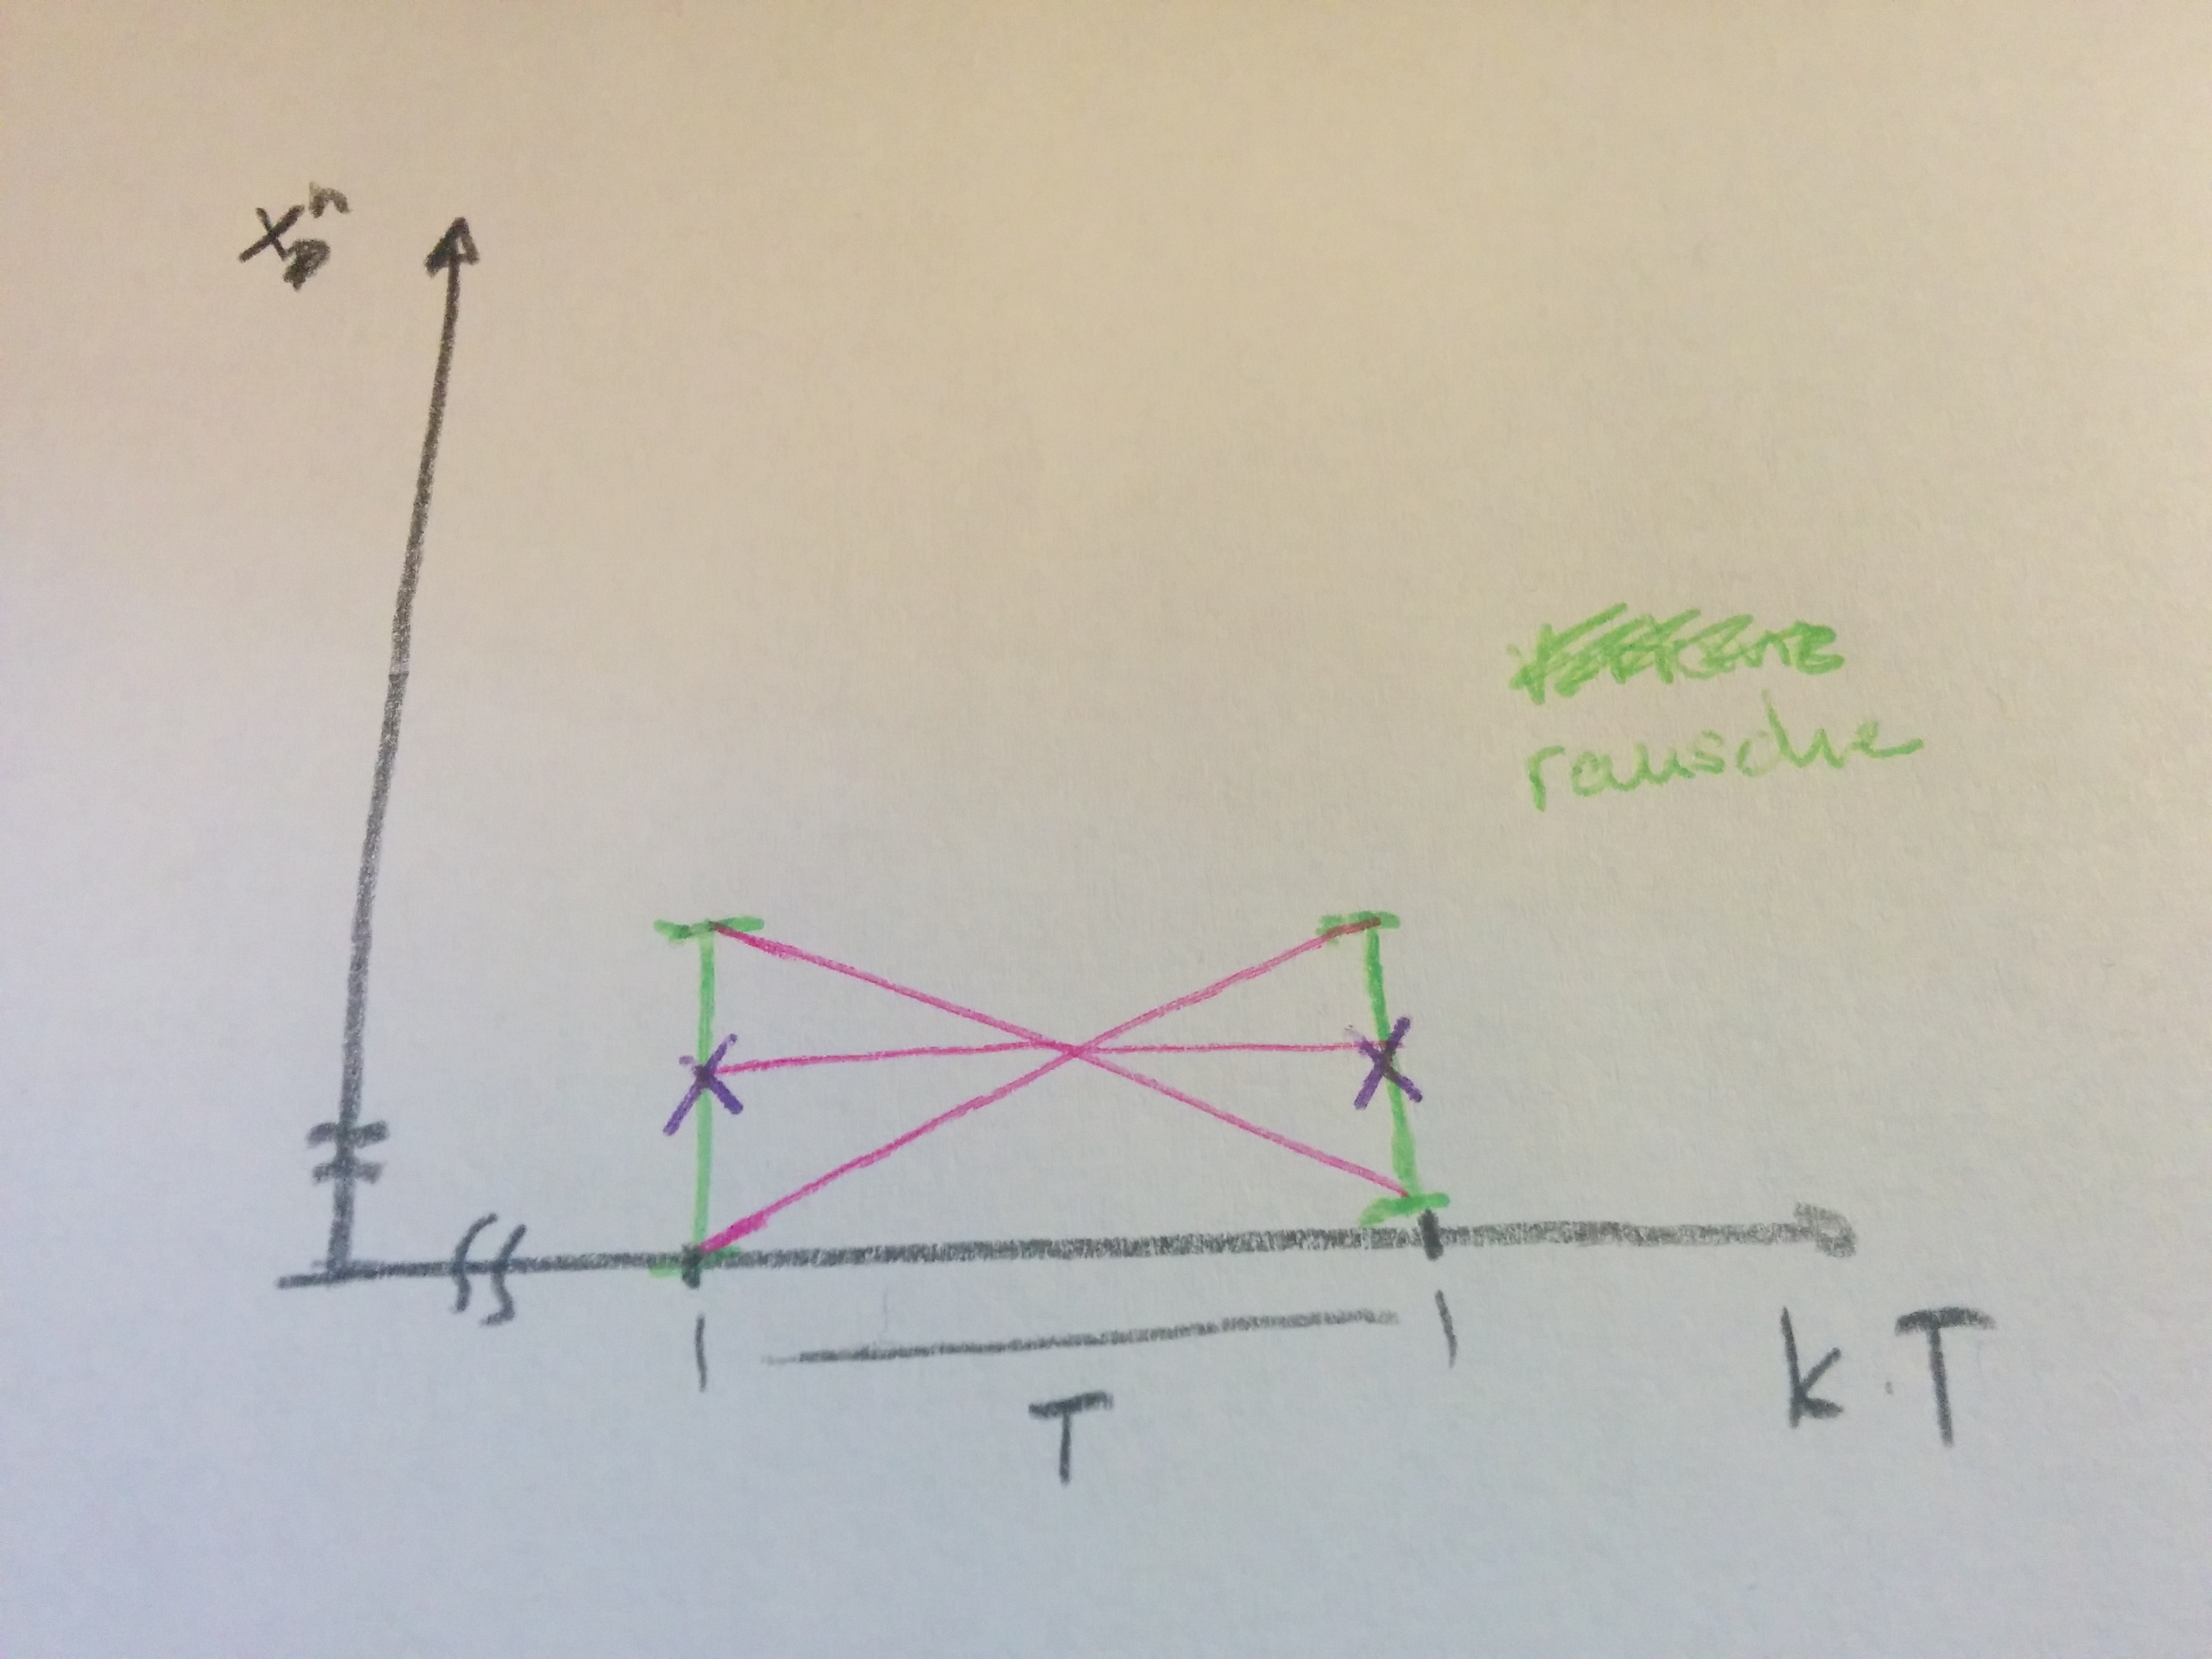
\includegraphics[width=0.4\textwidth]{images/hoheVar}
 			\label{fig:VarPosVerschHohe}
 		}
 		\hspace{0.1\textwidth}
 		\subfloat[Gro�e Positionsverschiebung, geringe Varianz]{
 			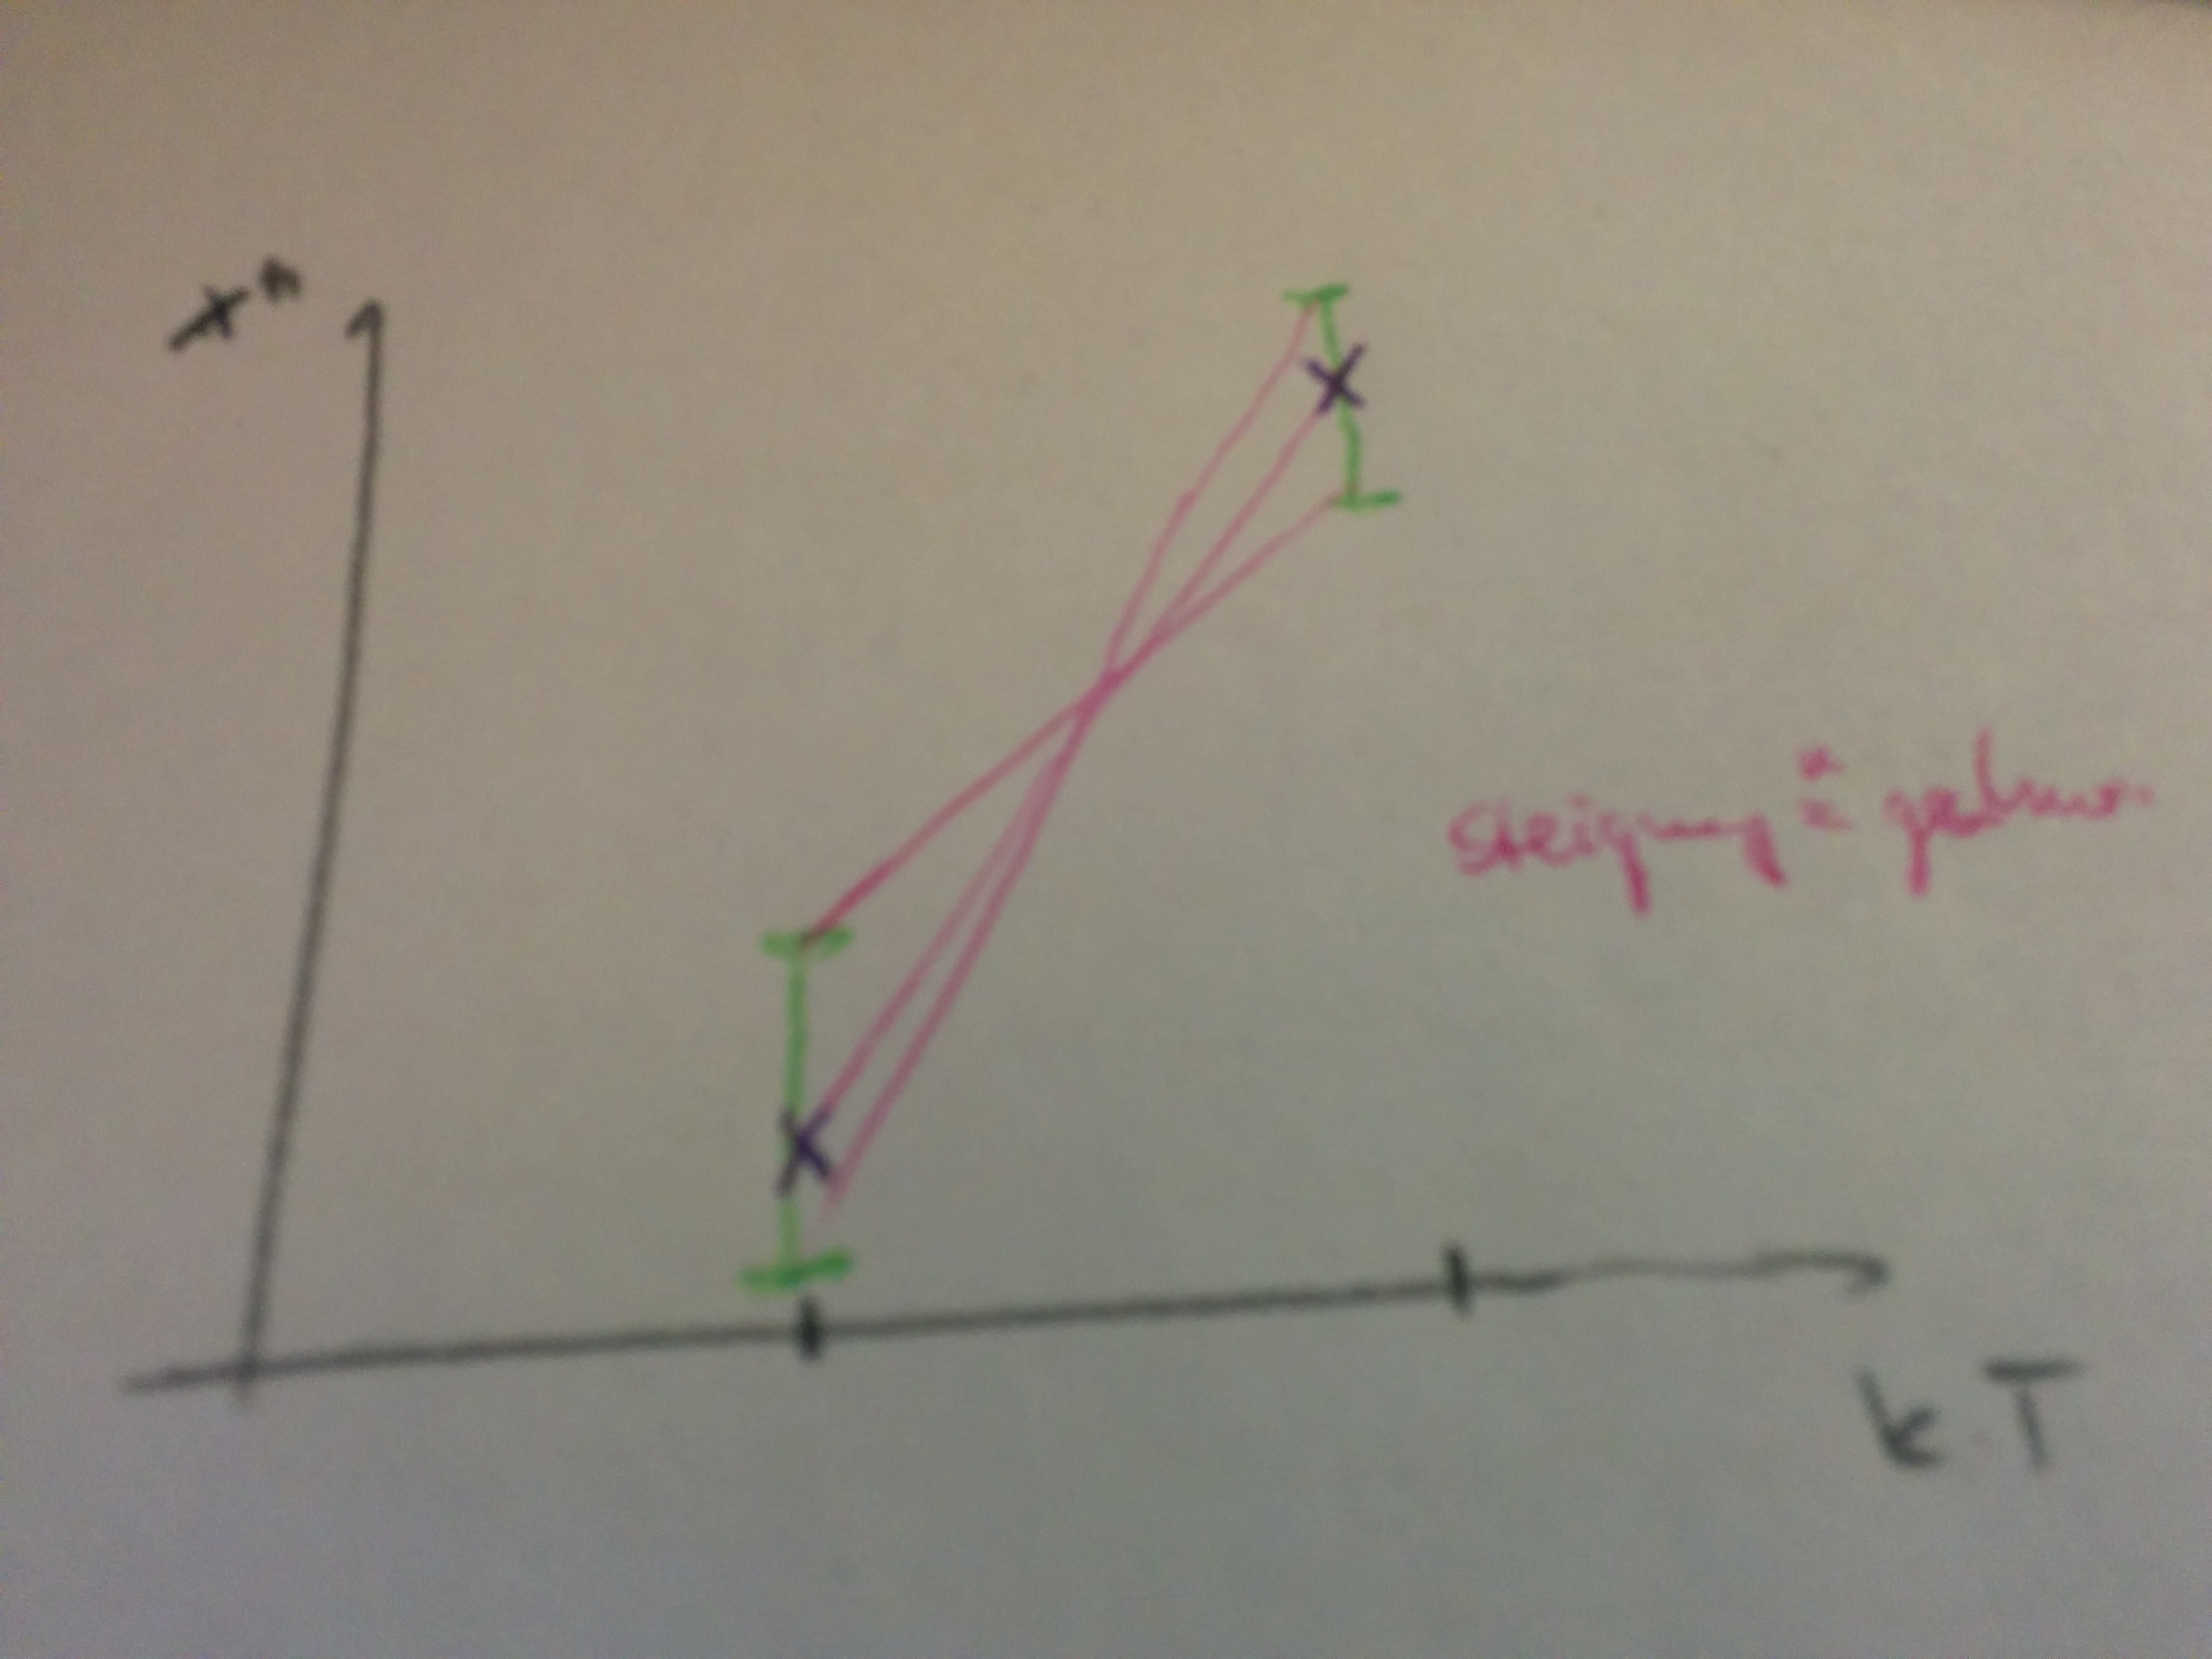
\includegraphics[width=0.4\textwidth]{images/kleineVar}
 			\label{fig:VarPosVerschNierdrig}
 		}
 	}	
 	\caption[Auswirkung der Positionsverschiebung auf Varianz der Geschwindigkeit]{Auswirkung der Gr��e der Positionsverschiebung innerhalb eines Sch�tzwertes auf die Varianz der Geschwindigkeitssch�tzung}
 	\label{fig:VarPosVersch}
 \end{figure}
 Geht man davon aus, das die Frequenz des Rauschanteils oberhalb des Frequenzbades der Positions�nderungen liegt. Kann das Nutzsignal mittels eines Tiefpassfilters vom Rauschanteil getrennt werden. Das Tiefpassfilter l�sst sich dabei mittels eines rekursiven \gls{iir}-Filters realisieren \cite{des14}. Die gefilterte Geschwindigkeit $ \hat{v}^n_k $ h�ngt dabei nicht nur von vorherigen Messwerten $v^n_k $  sondern auch von den vorherigen Filterergebnissen.
 \begin{equation}
 \hat{v}^n_k = \sum\limits_{j = 0}^{n}a_j \cdot v^n_{k-j}+ \sum\limits_{i = 1}^{n}b_j \cdot \hat{v}^n_{k-i}
 \label{eq:filter}
 \end{equation}
 Mittels der Koeffizienten $ a_j $ und $ b_i $ kann nun das gew�nschte Filterverhalten, zum Beispiel das eines Butterworth-Filters, mit der ben�tigten Grenzfrequenz realisiert werden. Die Ordnung $ n $ des Filter beschreibt wie viele der vorangegangenen Messwerten in die Filterung mit einzubeziehen sind. Beim Design des Filters m�ssen jedoch Kompromisse zwischen Zeitverz�gerung, Phasenverzerrung, D�mpfung und Stoppbandeigenschaften getroffen werden. F�r die Folgeregelung ist es dabei Wichtig, das die beiden erste genannten Kriterien m�glichst gering ausfallen. Ist dies nicht der Fall, wirkt es destabilisierend auf den Regler. 
 
 Des weiteren lassen sich Aufgrund der geringe Updaterate von $ 40 Hz $ der Positionsdaten, die Dynamik des Quadrocopters und das Positionsrauschen Spektral nicht von einander trennen. M�chte man also das Positionsrauschen unterdr�cken, werden auch schnelle Positions�nderungen des Quadrocoptes weg gefiltert. F�r die hohe Dynamik des Quadrocopters ist die Anwendung eines Tiefpassfilter mit Grenzfrequenz nicht m�glich. Gesucht ist nun eine Methode, die f�r Fl�ge mit geringer Dynamik die Varianz der Geschwindigkeitssch�tzung verursacht durch Positionsrauschen m�glichst stark verringert. Gleichzeitig jedoch der Hohen Dynamik des Quadrocopters folge leisten kann.  
 
 \subsection{Geschwindigkeitsbestimmung �ber die Methode First-Order Adaptive Windowing }
 \label{subsec:adaptwind}
 (Hier fehlt 1kHz und Position zwar h�hrer Abtastrate verf�gbar, Fehler drifftet durch doppelte Integration zu schnell zu weit weg)
 Wie schon in Kaptiel \ref{subsec:abpos} erkannt, nimmt die Varianz der Geschwindigkeitssch�tzung ab je weiter die Positionswerte auseinander liegen. Hierf�r sei auf Grafik \ref{fig:VarPosVerschNierdrig} verwiesen. Der gleiche Effekt tritt auf, je mehr Abtastschritte $ n $ der f�r die Eulerapproximation verwendete Bezugspunkt $ P^n_{k-n} $ in der Vergangenheit liegt. 
 \begin{equation}
 \hat{v}^n_k = \frac{P^n_k-P^n_{k-n}}{nT_l}=
 \label{eq:v_eul_n}
 \end{equation}
 Dabei ist die Verwendung der Bezugsposition $ P^n_{k-n} $ gleichzusetzen mit der Mittlung der letzten $ n $ Geschwindigkeitssch�tzungen ($ v^n_k,v^n_{k-1},\cdots,v^n_{k-1} $) mittels (\ref{eq:v_eul}). Deshalb spricht man auch von Fensterung beziehungsweise Windowing. Siehe zur Veranschaulichung Abbildung~\ref{fig:Fensterung}. Vergr��ert man das Fenster hat das eine �quivalente Wirkung wie die Reduzierung der Abtastrate.
  \begin{figure}
  	\centering
  	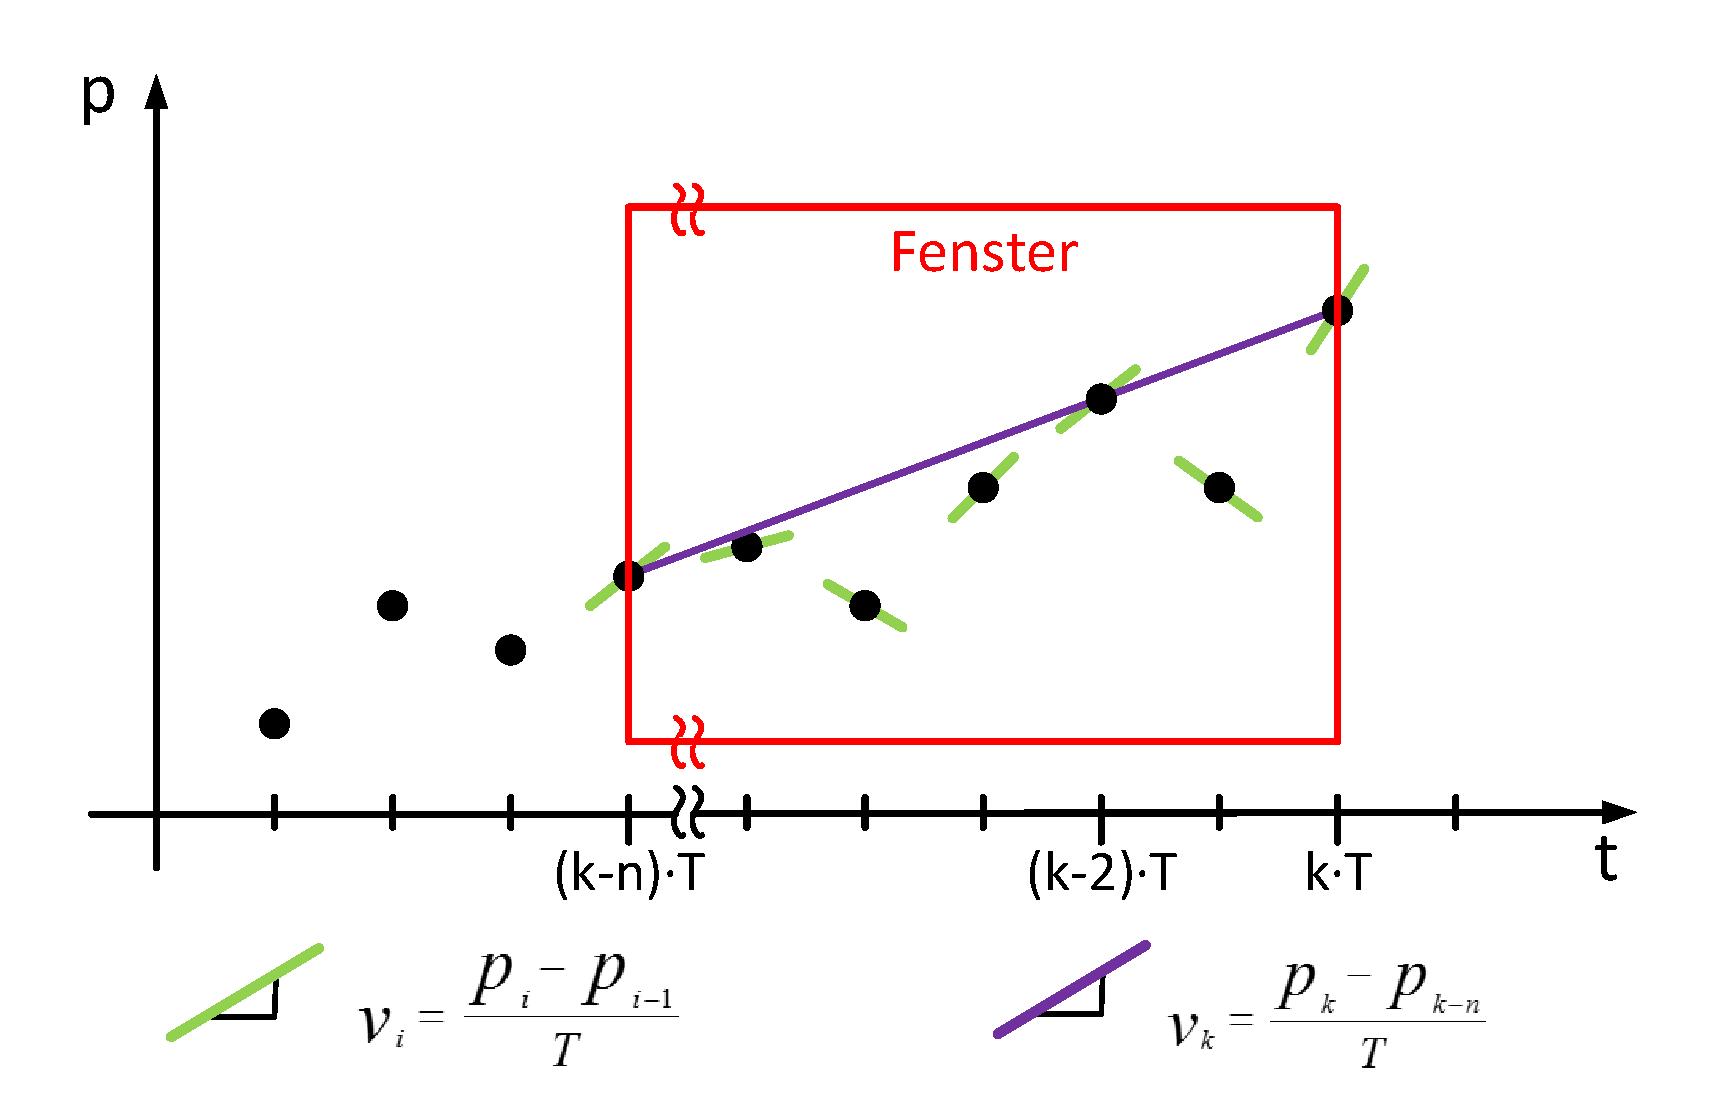
\includegraphics[width = \textwidth]{images/wind_avg}
  	\caption[Fensterung]{Fensterung} %
  	\label{fig:Fensterung}
  \end{figure}
 Das Windowing verh�lt sich wie ein Filter. So f�hrt ein gro�es Fenster bei geringen Dynamiken zu einer sehr pr�zisen Geschwindigkeitssch�tzung durch Rauschunterdr�ckung. Sch�tzungen f�r Hochfrequenter Bewegungen des Quadrocopter werden jedoch stark ged�mpft und Zeitverz�gert ausgegeben, womit die Verl�sslichkeit der Sch�tzung abnimmt. Es wirkt somit �hnlich wie das Filter (\ref{eq:filter}). Allerdings mit dem Vorteil, das Filterverhalten nur �ber eine Parameter einstellbar ist. Der Fenstergr��e $ n $. So sollte das Window klein sein, wenn der Quadrocopter Hochfrequente �nderungen der Bewegung vornimmt, damit die abrupten Geschwindigkeits�nderungen m�glichst unged�mpft erfasst werden. Bei geringen Dynamiken soll die Fenstergr��e jedoch zunehmen, wodurch der Einfluss des Positionsrauschens minimiert werden soll. 
   \begin{figure}
   	\centering
   	\includegraphics[width = \textwidth]{images/End-fit-foaw}
   	\caption[End-fit \gls{foaw}]{End-fit \gls{foaw}} %
   	\label{fig:foaw}
   \end{figure}
 Dabei muss die Anpassung der Fenstergr��e online und f�r jeden Punkt Abh�ngig der Achse des n-frame separat erfolgen. Im Paper \cite{adaptWin} wird daf�r die Methode des \gls{foaw} vorgestellt. Diese Besagt, existiert eine Grade zwischen den Positionswerten $ p^n_k $ und $ p^n_{k-n} $ einer Achse, die alle $ n $ Punkte innerhalb einer Tolerenz $ \pm d $ schneidet, stellt die Steigung dieser und somit die Geschwindigkeit einen optimalen Kompromiss zwischen Rauschunterdr�ckung (Pr�zision) und Verl�sslichkeit dar. Die m�glichen Sch�tzwerte f�r die Geschwindigkeit abh�ngig von der Fenstergr��e $ n $ und der Toleranz $ d $ sind im folgenden Datensatz dargestellt.
 
 \begin{equation}
 \hat{v}_k \in [\frac{p^n_k-p^n_{k-n}}{n T_l}-\frac{2d}{n T_l}, \frac{p^n_k-p^n_{k-n}}{n T_l}-\frac{2d}{n T_l}]
 \end{equation}
  Die Toleranz $ d $ ist dabei durch den Betrag der maximalen Rauschabweichung festgelegt und somit als Konstante zu sehen.
 \begin{equation}
 d = ||r_{max}||
 \end{equation}
Zu erkennen ist, das die Varianz der Sch�tzung f�r eine steigende Fenstergr��e $ n $ abnimmt. Somit ist ausgehend von der aktuellen Position $ p^n_k $ die maximale m�gliche Fenstergr��e $ n = max\{1,2,3,\dots\} $ zu ermitteln f�r die gilt,
\begin{equation}
|p^n_{k-i} - \hat{p}^n_{k-i}|\le d \hspace{1.5cm}\forall i \in \{1,2,\dots,n\}
\label{eq:toleranz}
\end{equation} 
Dabei entspricht $ \hat{p}^n_{k-i} $ den Punkte auf der approximierenden Geradengleichung.
\begin{equation}
\hat{p}^n_{k-i} = a_n + b_n \cdot(k-i) T_l
\label{eq:gradengl}
\end{equation}
In \cite{adaptWin} ist dazu ein iterativer Algorithmus zur L�sung dieses Problems beschrieben. Dabei sind die Parameter der Geradengleichung (\ref{eq:gradengl}) wie folgt parametriert.
\begin{equation}
a_n =\frac{k \cdot p^n_{k-i} + (n-k)p^n_{k}}{n}
\label{eq:a_n}
\end{equation}
\begin{equation}
b_n =\frac{p^n_{k} - p^n_{k-n}}{n T_l}
\label{eq:b_n}
\end{equation}



Da die Steigung $ b_n $ aus den zwei R�ndern des Fensters gebildet wird, spricht man von der End-fit-\gls{foaw}.  


Der Ablauf der des Interationsalgorithmus sieht dann wie folgt aus.

\begin{itemize}
	\item \textbf{Schritt 1:} Man verschiebt die Zeitachse so, dass f�r den Zeitpunkt des neusten Wert $ p^n_k $ gilt $ t_k = k\cdot T_l = 0 $. Die Folge ist eine vom Faktor $ k $ unabh�ngige Geradengleichung.
	\begin{equation}
	\hat{p}^n_{k-i} = a_n + b_n \cdot(-i) \cdot T_l
	\label{eq:gradengl_t0}
	\end{equation}
	F�r die gilt,
	 \begin{equation}
	a_n = p^n_k
	\end{equation}
	und $ b_n  $ weiterhin �ber (\ref{eq:a_n}) berechnet werden kann. Vorteil, es muss jeweils nur die Steigung neu berechnet werden.
	\item \textbf{Schritt 2:} Fenstergr��e j = 1.
	\item \textbf{Schritt 2:} Berechnung des Parameters $b_j $ (\ref{eq:b_n}) der Geradengleichung (\ref{eq:gradengl_t0}) in Abh�ngigkeit der Fenstergr��e $ j $.
	\item \textbf{Schritt 3:} �berpr�fen ob die berechnete Gerade alle im Fester befindlichen Punkte $p^n_{k-i} i \in \{1,2,\dots,j\} $ innerhalb  der Toleranz passiert. Bedingung (\ref{eq:toleranz}) 
	\item \textbf{Schritt 4:} Ist Schritt 3 erf�llt, inkrementiere die Fenstergr��e $ j =j+1 $ und gehe zu Schritt 2. Wenn Bedingung nicht erf�llt, ist die Steigung der vorhergegangen Geradengleichung als Sch�tzwert der Geschwindigkeit auszugeben. 
	\begin{equation}
	 \hat{v}_k = b_{j-1}=b_n
	\end{equation} 
	Die maximale Fenstergr��e $ n $ entspricht f�r Position $ p^n_{k} $  somit $ n = j-1 $ 
\end{itemize} 

 Dieser Vorgang wird f�r jeden Aktualisierung  $ k = k+1 $ des Positionswert $ p^n_{k} $ neu gestartet. Zur Veranschaulichung ist der Algorithmus noch einmal in einen Flussdiagramm (Abbildung \ref{fig:flussfoaw}) dargestellt.  

 \begin{figure}
 	\centering
 	\includegraphics[width = \textwidth]{images/Platzhalter}
 	\caption[Flussdiagramm \gls{foaw}]{Flussdiagramm \gls{foaw}} %
 	\label{fig:flussfoaw}
 \end{figure}
 Die End-fit-\gls{foaw} verwendet f�r den Sch�tzvorgang die zwei Endpunkte des Fensters. In \cite{adaptWin} wird deshalb noch die Best-fit\gls{foaw} vorgestellt. Dabei wird die Steigung, �ber die Methode der des kleinsten quadratischen Fehler bestimmt. Das bedeutet f�r die zeitnormierte Geradengleichung ist eine Steigung $ b_n $ gesucht f�r die die Summe der Fehlerquadrat $ e^2 $ ein Minimum aufweist.  
 \begin{equation}
 e_{min}^2 = min \sum\limits_{i=0}^{n}(p^n_{k-i} - \hat{p}^n_{k-i})^2
 \label{eq:quade}
 \end{equation}
 mit
 \begin{equation}
\hat{p}^n_{k-i} = p^n_{k} - b_n \cdot i \cdot T_l 
 \end{equation}
Um das Minimum der Fehlergleichung (\ref{eq:quade}) in Abh�ngigkeit der Steigung bestimmen zu k�nnen, muss diese nach $ b_n $ abzuleiten. Da es sich um eine quadratische Gleichung handelt, weist der Fehler Tiefpunkt auf wenn diese Ableitung Null ergibt.
\begin{equation}
\frac{d e^2}{d b_n}=0
\end{equation}
L�st man unter dieser Bedingung die Ableitung nach $ b_n $ auf. Erh�lt man die Steigung die die Summe der kleinsten quadratischen Fehler aufweist.
\begin{equation}
b_n = \frac{(n\sum\limits_{ i=0}^{n}y_{k-1}-2\sum\limits_{i=0}^{n} i\cdot y_{k-1})\cdot 6 }{T_l n(n+1)(n+2)}
\end{equation}
Nun ist die Steigung allgemeing�ltig f�r variable Fenstergr��en bestimmt. Die Umsetzung der best-fit-\gls{foaw} in der Software erfolgt nach dem gleichen Schema wie bei der end-fit-\gls{foaw}. Einziger Unterschied, zur Berechnung der Steigung $ b_n $ wir die Gleichung verwendet. Das Ergbnis ist eine pr�zisere Sch�tzung bei gleichbleibender Zuverl�ssigkeit der Messung. Beide Methoden sind jedoch anf�llig gegen sogenannte Outliner. Einzelne Signalwerte die eine h�heren Fehler als die maximale durch das Rauschen verursachte Abweichung $ d $ aufweisen. Outliner lassen sich jedoch sehr einfach durch eine robuster Abbruchkriterium in Schritt 3 bek�mpfen. So gilt die Bedingung (\ref{eq:toleranz}) erst dann f�r nicht bestimmt, wenn zwei aufeinanderfolgende Werte das Kriterum nicht erf�llen. Erst dann wird die Vergr��erung des Fensters gestoppt. Diese Variante nennt sich best-fit-\gls{foaw}-R.
 \begin{figure}
 	
 	\centering{
 		\subfloat[Positionsignal]{
 			\includegraphics[width=0.5\textwidth]{images/adap_position}
 			\label{fig:adapt_pos}
 		}
 		\subfloat[Ableitung (Kapitel \ref{subsec:abpos}) vs. endfit-\gls{foaw}]{
 			\includegraphics[width=0.5\textwidth]{images/adap_dtvsendfit}
 			\label{fig:adapt_ablvsend}
 		}\\
 		\subfloat[endfit-\gls{foaw} vs. bestfit-\gls{foaw}]{
 			\includegraphics[width=0.5\textwidth]{images/adap_endfitvsbestfit}
 			\label{fig:adapt_endvsbest}
 		}
 		\subfloat[bestfit-\gls{foaw} vs. bestfit-R-\gls{foaw}]{
 			\includegraphics[width=0.5\textwidth]{images/adap_bestfitvsbestfitr}
 			\label{fig:adapt_bestvsbestr}
 		}
 		}
 		
 	\caption[Messergebnis f�r \gls{foaw}]{Vergleich der Filterergebnisse f�r \gls{foaw}}
 	\label{fig:adap_vergleich}
 \end{figure}



Die Methoden des \gls{foaw} bietet eine sehr M�glichkeit die Geschwindigkeit auf Basis eines verrauschten Positionssignal zu ermitteln. Problematisch ist jedoch die geringe Abtastrate von $ 40 Hz $ des Lasers. Schon bei Fl�gen bei mittlerer Dynamik f�hrt dies dazu, das die Fenstergr��e stark reduziert wird. Somit auch der Einfluss des Positionsrauschens stark zunimmt. Somit kann selbst diese Konzept limitiert durch die Tastrate des Lasers der Dynamik des Quadrocopters nicht nachkommen. Es ist somit klar das eine Methode ben�tigt wird, die Position und Geschwindigkeit in einer h�hren Taktrate zur Verf�gung stellt. Gleichzeit m�ssen beide Signale ausreichend Rauschunterdr�ckt sein. 

 \subsection{Bestimmung der Zust�nde mittels eines Fusionsfilter}
 \label{subsec:Fusionsfilter}
 Wie aus den oberen Kapitel zuerkenne wird keine der Methoden den zuvor gestellten Anspr�che gerecht. So erf�llt die Integration der Beschleunigung (Kapitel \ref{subsec:Vimu}) zwar das Kriterium zur Erh�hung der Taktrate. Beschleunigungsmesswerte werden in einem Takt von $ 1 kHz $ zur Verf�gung gestellt. Doch durch den Bias des Beschleunigungssensors, divergieren innerhalb k�rzester Zeit die gesch�tzten Zust�nde von den realen Zust�nden. Dieses Ph�nomen tritt bei den Anwendungen Kaptiel und Kapitel nicht auf. Der Grund, sie beziehen sich auf die vom Laser berechneten Positionswerte. Die Abweichungen dieser Zustandswerte befinden sich dabei in einem konstanten Rahmen um die tats�chliche Position. Diese Positionsrauschen sorgt bei der Geschwindigkeitssch�tzung �ber die Ableitung der Positionswerte daf�r, dass das errechnete Geschwindigkeitssignal ebenfalls einen Rauschanteil aufweist. Diesen Rauschanteil zu minimieren ist Ziel der \gls{foaw} Methode. Aufgrund der geringen Abtastfrequenz von $ 40Hz  $ kann dieser Ansatz der hohen Dynamik nicht folge leisten. Schon f�r geringen Dynamiken ist die Fenstergr��e stark dezimiert und somit auch die Rauschunterdr�ckung. Das Ergebnis, Bechleunigungssensor der \gls{imu} und Laser jeweils f�r sich bieten keine ausreichende Zustandswerte. Abhilfe, Fusion beider Sensordaten mittels eines Fusionsfilters. Dabei sorgen die Beschleunigungswerte mit ihrer hohen update Rate von $ 1 Khz $ f�r eine schnelle Reaktionsf�higkeit und tragen somit der Dynamik des Quadrocopters sorge. Die Positionsdaten des Laser indes verhindern ein Abdriften der Sch�tzwerte. Somit stellen sie die Zuverl�ssigkeit der Fusionsergebnisse sicher. 
 
Das auf dem \gls{hlp} implementierte Fusionsfilter basiert auf einem Leunberger Beobachter\cite{Achtelik11}. Dieser besteht aus einen linearen Streckenmodell dessen Zust�nde $ \hat{x} $ mittels eines Korrekturterms ($ L\cdot (y-\hat{y})$) auf die Zust�nde $ x $ der Regelstrecke einschwingen. Die Zustandsdifferenzialgleichung eines Luenberger Beobachter stellt sich in allgemeiner Form  \cite{regB12} wie folgt dar.
\begin{equation}
\begin{split}
\dot{\hat{x}} &= A \cdot \hat{x}+ L \cdot (y-\hat{y}) + B \cdot u\\
\hat{y} &= C \cdot \hat{x}
\end{split}
\label{eq:algbeo}
\end{equation} 
Dabei entspricht $ A $ der Dynamikmatrix, $ B $ dem Eingangsmatrix und $ C $ dem Ausgangsmatrix des linearen Streckenmodells. Aufgrund der Inversion, ist das Bewegungsmodell f�r jede Achse im n-frame, als Integrationsglied 2.Ordnung gegeben (Abbildung \ref{fig:drIntket}). Dabei entspricht die Eingangsgr��en $ u $ den ins n-frame transformierten Beschleunigungswerten der \gls{imu}. Da die Ketten entkoppelt sind, muss der Beobachter nicht f�r alle drei Ketten gleichzeitig entworfen werden. Somit ist es ausreichen eine Integrationsglied 2.Ordnung als Streckenmodell heranzuziehen. Weiterhin ist bekannt, das die Beschleunigungswerte der \gls{imu} einen Bias aufweisen. Nach \cite{mzr13} kann das Streckenmodell deshalb wie in Abbildung \ref{emod} erweitert werden. 
   \begin{figure}
   	\centering
   	\includegraphics[width = \textwidth]{images/erwModell}
   	\caption[Erweitertes Streckenmodell]{Erweitertes Streckenmodell} %
   	\label{fig:emod}
   \end{figure}
Dieses erweiterte Modell ist �ber Zustandsdifferenzialgleichung (\ref{eq:emod}) beschreiben
\begin{equation}
\begin{split}
\dot{x} &= \underset{A}{\begin{bmatrix} 
	0&	1&	0\\
	0&  0&  1\\
	0&	0&  0
	\end{bmatrix}} \cdot x+ \underset{B}{\begin{bmatrix}
	0\\
	1\\
	0
	\end{bmatrix}} \cdot u\\
y &= \underset{C}{\begin{bmatrix}
	1& 0& 0
	\end{bmatrix}} \cdot x
\end{split}
\label{eq:emod}
\end{equation} 
mit,
\begin{equation}
\hat{x} = \begin{bmatrix}
p^n&	v^n& 	b
\end{bmatrix}^T
\end{equation}
Anhand von (\ref{eq:algbeo}) folgt daraus f�r den Beobachter.
\begin{equation}
\begin{split}
\dot{\hat{x}} &= \underset{A}{\begin{bmatrix} 
	0&	1&	0\\
	0&  0&  1\\
	0&	0&  0
	\end{bmatrix}} \cdot \hat{x}+ \underset{L}{\begin{bmatrix}
	l_1\\
	l_2\\
	l_3
	\end{bmatrix}} \cdot (y-\hat{y}) + \underset{B}{\begin{bmatrix}
	0\\
	1\\
	0
	\end{bmatrix}} \cdot u\\
\hat{y} &= \underset{C}{\begin{bmatrix}
	1& 0& 0
	\end{bmatrix}} \cdot \hat{x}
\end{split}
\end{equation} 
mit,
\begin{equation}
\hat{x} = \begin{bmatrix}
\hat{p}^n&	\hat{v}^n& 	\hat{b}
\end{bmatrix}^T
\end{equation}
Die Elemente der Beobachtermartix $ L $ sind so zu parametrieren das die Fehlerdynamik das gew�nschte Einschwingverhalten aufweist. Da der Zustandsfehler $ \tilde{x} = x-\hat{x} $ gilt, ergibt sich f�r die Dynamik des Zustandsfehlers
\begin{equation}
\dot{\tilde{x}}=\dot{x}-\dot{\hat{x}}=(A-LC)\cdot \tilde{x}
\end{equation}
Um diese mittels Polvorgabe einstellen zu k�nnen, muss charakteristische Polynom gebildet werden \cite{regB12}.
\begin{equation} 
N(s)=\det(A-LC)
\end{equation}
ergibt f�r das erweitere Zustandsmodell,
\begin{equation} 
N(s)=s^3+l_1\cdot s^2+l_2 \cdot s + l_3
\end{equation}
Anhand dieses Polynom sind Koeffizienten der Beobachtermatrix $ L $ nach Kapitel \ref{subsec:polvor} �ber Polvorgabe vorgebbar. 
  \begin{figure}
  	\centering
  	\includegraphics[width = \textwidth]{images/Platzhalter}
  	\caption[Beobachter]{Strukturbild Beobachter} %
  	\label{fig:strucB}
  \end{figure}
 
 \begin{figure}
 	
 	\centering{
 		\subfloat[Einspeisung]{
 			\includegraphics[width=0.5\textwidth]{images/ua}
 			\label{fig:bo_ua}
 		}
 		\subfloat[Einschwingverhalten Bias]{
 			\includegraphics[width=0.5\textwidth]{images/bias}
 			\label{fig:bo_bias}
 		}\\
 			\subfloat[Beschleunigung]{
 				\includegraphics[width=0.5\textwidth]{images/beschl}
 				\label{fig:bo_beschl}
 			}
 			\subfloat[Geschwindigkeit]{
 				\includegraphics[width=0.5\textwidth]{images/geschw}
 				\label{fig:bo_geschw}
 			}\\
 			\subfloat[Position]{
 				\includegraphics[width=0.5\textwidth]{images/Position}
 				\label{fig:bo_pos}
 			}
 		}	
 	\caption[Simulation Beobachter]{Simulationsergebnisse f�r das Fusionsfilter}
 	\label{fig:bo_sim}
 \end{figure}
  
  \begin{figure}
  	
  	\centering{
  		\subfloat[Positionsignal]{
  			\includegraphics[width=0.5\textwidth]{images/adap_position}
  			\label{fig:bo_adapt_pos}
  		}
  		\subfloat[Ableitung (Kapitel \ref{subsec:abpos}) vs. Beobachter]{
  			\includegraphics[width=0.5\textwidth]{images/obs_vxvsob}
  			\label{fig:bo_dvdtvsbo}
  		}
  	}	
  	\caption[Verbesserung des Fusionsfilter im Vergleich \gls{foaw}]{Verbesserung des Fusionsfilter im Vergleich \gls{foaw}}
  	\label{fig:bo_sim}
  \end{figure} 
 
\chapter[Flugversuche]{Verifizierung der Positionsregelung am realen System}
\label{chap:Flugversuche}
Nach dem die Funktionsf�higkeit der von \gls{asctec} und ETH-Z�rich entworfenen Positionsregelung mittels Herleitung der einzelnen Komponenten sowie einer abschlie�enden Simulation des Gesamtsystems (Kapitel \ref{sec:sim_posreg}) in der Theorie beweisen ist, fokussiert sich diese Kapitel \ref{chap:Flugversuche} auf die Verifizierung der Regelung am realen System. So gilt es zu darauf zu achten ob die Zeitkonstante der Lagerregelung, die in der Modellbildung vernachl�ssigt worden ist, eine Auswirkung auf die Positionsregelung hat. Auch zeigen wird sich ob die Positionsbestimmung mittels eines Lasers anhand der in Kapitel \ref{chap:2Dpositionsbestimmung} beschrieben orthogonalen Projektion sowie das scanmatching-Verfahren anwendbar ist. 

Daf�r wird in Kapitel \ref{sec:anflugKoor} eine Messung untersucht, bei der der Positionsregelung eine neue Koordinate �bergeben wird, in die der Quadrocopter �berf�hrt werden soll. Im Anschlie�end Kapitel \ref{sec:geschwReg} wird Bezugnehmend auf das urspr�ngliche Thema der Arbeit, der Geschwindigkeitsregelung des Quadrocopter, die Funktionsf�higkeit der Positionsregelung als eben diese Geschwindigkeitsregelung dargelegt.



\section{Anflug einer Koordinate im Raum}
\label{sec:anflugKoor}


\section{Geschwindigkeitsregelung }
\label{sec:geschwReg}





 
\chapter[Zusammenfassung und Ausblick]{Zusammenfassung und Ausblick}
\label{chap:zusammenfassungAusblick}

\section{Zusammenfassung}
\label{sec:zusammenfassung}
Im Rahmen dieser Masterthesis wurde eine Positions- und Geschwindigkeitsreglung, basierend auf einem Onboardlokalisierungssystem, mittels eines Laserscanners auf dem Pelican Quadrocopter der Firma \gls{asctec} implementiert. Zur Lokalisierung und Regelung wurden dabei bereits entwickelte Funktionsbausteine zu einem funktionierenden Gesamtsystem zusammengef�gt. So ist der Schwerpunkt darauf ausgelegt, die Theorie und die Konzepte dieser Bausteine offenzulegen.

Begonnen wurde mit der Lokalisierung des Quadrocopters. Dort wird aufgezeigt, wie der Einfluss der Neigungswinkel auf die Entfernungsmessung mittels einer orthogonalen Projektion der Messwerte auf die horizontale Ebene des Raumes eliminiert wird. Die Grundvoraussetzung f�r den bei Positionsbestimmung zum Einsatz kommenden Scanmatching-Algorithmus, dessen Funktionsweise in dieser Arbeit ebenfalls mathematisch dargelegt ist.

Im n�chsten Schritt erfolgte die Validierung der von \gls{asctec} in Verbindung mit der ETH-Z�rich entwickelten Positionsregelung. Angelehnt an die Funktionsbeschreibung des Reglers in \cite{Achtelik11} bestand die Herausforderung darin, den dort beschriebenen Aufbau der Regelung mittels Literaturverweise, der Herleitung der verwendeten Regelalgorithmen sowie anhand von Simulationsbeispielen zu legitimieren. Zus�tzlich wurde aufgezeigt, �ber welche Stellschrauben die Komponenten der Regelung zu parametrieren sind.

Nachdem die Legitimierung der Positionsregelung mit einer abschlie�enden Simulation des Gesamtsystems in der Theorie bewiesen war, erfolgten Flugversuche mit dem Quadrocopter. Diese belegten die Funktionsf�higkeit der Positionsregelung als auch der Geschwindigkeitsregelung in der Praxis, was auch aus den in dieser Arbeit ver�ffentlichen Messdaten zweier Flugversuche hervorgeht. Allerdings stellte sich dabei heraus, dass es kleine Defizite bei der Positionsbestimmung mittels des Lasers zu beheben gibt. Vereinzelt zeigte sich, dass �ber kurze Zeitr�ume von circa einer Sekunde die Position des Quadrocopters nicht aktualisiert wird. Dies f�hrte zu einer Fehlinterpretation der Positionsregelung �ber den Zustand des Quadrocopters, was im ung�nstigsten Fall zum Absturz des Flugobjektes f�hren kann. Hier gilt es im Anschluss dieser Arbeit Nachforschungen zur Ergr�ndung der Ursache dieser Positionsfehlstellen anzustellen. 

\section{Ausblick}
\label{sec:ausblick}
Ungeachtet der aktuell bekannten Defizite bei der Positionsbestimmung ist die Empfehlung zun�chst die H�hensch�tzung von Jan Kallwies \cite{JanKal13} auf dem Quadrocopter zu integrieren. Dies w�rde nicht nur dazu f�hren, dass mittels der Positionsregelung  Koordinaten in einem dreidimensionalen Raum vollst�ndig autonom angeflogen werden k�nnen, sondern er�ffnet gleichzeitig neue M�glichkeiten bei Positionsbestimmung mittels des Lasers. So kann unter Ber�cksichtigung der Flugh�he zur Bestimmung der Position ein 3D-\gls{slam}-Algortihmus eingesetzt werden. Diese Art der Lokalisierung hat gegen�ber des simplen Scanmatching-Verfahren den Vorteil, dass es unabh�ngig von senkrechten Eigenschaften der Umgebung ist. Ob dies jedoch dazu f�hrt das keine L�cken in der Positionsbestimmung auftreten, ist nicht garantiert. Deshalb gilt es, sich zus�tzlich mit der Entwicklung eines Notlaufprogramms zu besch�ftigen. Dieses k�nnte so aufgebaut sein, dass es ausbleibende Aktualisierungen der Positionsdaten erkennt, alle von der Regelung geforderten Stellwinkel zur�ck nimmt und erst nach Erhalten neuer Positionswerte diese wieder freigibt. Gleichzeitig w�re eine akustische Warnung denkbar, so dass der Bediener im Ernstfall die Regelung komplett deaktivieren und das Flugsystem rechtzeitig manuell stabilisieren kann.

Alles in allem ist das Ziel mit dem Quadrocopter einer autonome Referenzplattform f�r das am Fraunhofer-Insitut f�r Integrierte Schaltungen entwickelte Lokalisierungssysteme durch diese Arbeit ein St�ck n�her ger�ckt.

%\chapter[Flugversuche]{Verifizierung der Positionsregelung am realen System}
\label{chap:Flugversuche}
Nach dem die Funktionsf�higkeit der von \gls{asctec} und ETH-Z�rich entworfenen Positionsregelung mittels Herleitung der einzelnen Komponenten sowie einer abschlie�enden Simulation des Gesamtsystems (Kapitel \ref{sec:sim_posreg}) in der Theorie bewiesen ist, fokussiert sich \DIFdelbegin \DIFdel{diese }\DIFdelend \DIFaddbegin \DIFadd{dieses }\DIFaddend Kapitel \ref{chap:Flugversuche} auf die Verifizierung der Regelung am realen System. So gilt es zu darauf zu achten\DIFaddbegin \DIFadd{, }\DIFaddend ob die Zeitkonstante der Lagerregelung, die in der Modellbildung vernachl�ssigt worden ist, eine Auswirkung auf die Positionsregelung hat. Ausweisen wird sich\DIFaddbegin \DIFadd{, }\DIFaddend ob die Positionsbestimmung mittels eines Lasers anhand der in Kapitel \ref{chap:2Dpositionsbestimmung} beschrieben orthogonalen Projektion sowie das scanmatching-Verfahren anwendbar ist. 

Daf�r wird in Kapitel \ref{sec:anflugKoor} eine Messung untersucht, bei der der Positionsregelung eine neue Koordinate �bergeben wird, in die der Quadrocopter �berf�hrt werden \DIFdelbegin \DIFdel{soll. Im anschlie�end }\DIFdelend \DIFaddbegin \DIFadd{kann. Im anschlie�enden }\DIFaddend Kapitel \ref{sec:geschwReg} wird bezugnehmend auf das urspr�ngliche Thema der Arbeit, der Geschwindigkeitsregelung des Quadrocopter, die Funktionsf�higkeit der Positionsregelung als eben diese Geschwindigkeitsregelung dargelegt.



\section{Anflug einer Koordinate im Raum}
Um die Messergebnisse mit \DIFdelbegin \DIFdel{denn }\DIFdelend \DIFaddbegin \DIFadd{denen }\DIFaddend der Simulation in Kapitel \ref{sec:sim_posreg} vergleichbar zu gestalten, entspricht die Ausgangskoordinate ($ x = 0$, $y = 0 $) als auch die Zielkoordinate ($ x = -2$, $y = 1 $) denen des Simulationsbeispieles. Des Weiteren stimmen die Parameter \DIFdelbegin \DIFdel{es Beobachter }\DIFdelend \DIFaddbegin \DIFadd{des Beobachters }\DIFaddend ($ L= \begin{bmatrix} 18 & 46 & 3.75 \end{bmatrix}^T $) sowie die der Positionsregelung ($ \tilde{c}_1 = 4 $, $ \tilde{c}_0 = 5 $, $ \tilde{c}_1 = 0.01 $) mit der in der Simulation verwendeten Parametrierung �berein. Zus�tzlich erfolgte auch hier die Ausrichtung des Quadrocopters so, dass die Orientierung des o-frames �ber den Zeitraum der Messung mit dem n-frame �bereinstimmt ($ \psi = 0 $). Damit ist hier ebenfalls die Achsenbewegung einem bestimmten Neigungswinkel zuzuordnen.   
\label{sec:anflugKoor}
 \begin{figure}
 	\centering
 	\includegraphics[width = .75 \textwidth]{images/real_xy}
 	\caption[Positionsverschiebung des Quadrocopters]{Positionsverschiebung des Quadrocopters} %
 	\label{fig:real_xy}
 \end{figure}

 Betrachtet man zun�chst den Verlauf des Referenzpfades in Abbildung \ref{fig:real_xy} und vergleicht diesen mit dem in der Abbildung \ref{fig:gessim_xy} dargestellten der Simulation, f�llt auf, \DIFdelbegin \DIFdel{das }\DIFdelend \DIFaddbegin \DIFadd{dass }\DIFaddend diese nicht den gleichen Verlauf aufzeigen. \DIFdelbegin \DIFdel{Erkl�ren l�sst sich das damit, das es }\DIFdelend \DIFaddbegin \DIFadd{Erkl�rung ist, dass es sich }\DIFaddend bei dem auf dem \gls{hlp} realisierte Referenzmodell nicht eins zu eins um \DIFdelbegin \DIFdel{den }\DIFdelend die in Paper \cite{Achtelik11} als auch in Kapitel \ref{sec:referenzmodell} vorgestellte Vorsteuerung handelt. Pr�ziser ausgedr�ckt\DIFaddbegin \DIFadd{, }\DIFaddend deutet das Messergebnis darauf hin, \DIFdelbegin \DIFdel{das }\DIFdelend \DIFaddbegin \DIFadd{dass }\DIFaddend die Vorsteuerung eine Trajektorie mit einer h�heren Stetigkeitsbedingung generiert \cite{mzr13}. Das bedeutet\DIFaddbegin \DIFadd{, }\DIFaddend der vorgegebene Pfad ist zweimal stetig differenzierbar und nicht nur einmal\DIFdelbegin \DIFdel{sowie }\DIFdelend \DIFaddbegin \DIFadd{, wie }\DIFaddend in Kapitel \ref{sec:referenzmodell} beschrieben. Zur Folge hat dies, dass der gew�nschte Beschleunigungsverlauf und \DIFaddbegin \DIFadd{die }\DIFaddend damit verbunden Vorgabe der Neigunswinkel stetig ist, d.h. keine spunghaften �nderungen gefordert werden. Best�tigt wird diese Annahme, wenn man den Verlauf der vorgegeben Neigungswinkel in Abbildung \ref{fig:real} mit den Winkel der Simulation (Abbildung \ref{fig:gessim}) vergleicht. 

 Untersucht wird jetzt die Flugbahn des Quadrocopter anhand der vom Beobachter gesch�tzten Positionsdaten in Abbildung \ref{fig:real_xy}. \DIFdelbegin \DIFdel{Zu erkennen }\DIFdelend \DIFaddbegin \DIFadd{Erkennbar }\DIFaddend ist, dass die Position des Quadrocopter ausgehend von einer inkonsistente Anfangsbedingung dank des Folgereglers zu \DIFdelbegin \DIFdel{Beginn }\DIFdelend \DIFaddbegin \DIFadd{beginn }\DIFaddend mit der Referenztrajektorie konvergiert. Ab der Koordinate $ x = -1 $ und $ y = 0.75 $ entfernt sich \DIFdelbegin \DIFdel{jedoch }\DIFdelend \DIFaddbegin \DIFadd{allerdings }\DIFaddend der Quadrocopter von dem vorgegebenen Pfad\DIFdelbegin \DIFdel{bevor er }\DIFdelend \DIFaddbegin \DIFadd{, bevor er sich }\DIFaddend schlie�lich �ber der Zielposition einschwingt. Um zu ergr�nden warum die Position des Flugsystems pl�tzlich vom Referenzpfad divergiert\DIFaddbegin \DIFadd{, }\DIFaddend ist der zeitliche Verlauf der Zust�nde f�r jede Achse zu untersuchen (\ref{fig:real}). Dabei l�sst sich anhand Abbildung \ref{fig:real_x} und Abbildung \ref{fig:real_y} erkennen, \DIFdelbegin \DIFdel{das }\DIFdelend \DIFaddbegin \DIFadd{dass }\DIFaddend kurz bevor der Quadrocopter den Referenzpfad schneidet, f�r circa eine Sekunde keine \DIFdelbegin \DIFdel{Positionspdates vom Laser zu }\DIFdelend \DIFaddbegin \DIFadd{Positionsupdates vom Laser zur }\DIFaddend Verf�gung stehen. Dies hat zur Folge\DIFdelbegin \DIFdel{das }\DIFdelend \DIFaddbegin \DIFadd{, dass }\DIFaddend der Sch�tzwert des Beobachters auf der letzten bekannten Position \DIFdelbegin \DIFdel{verharrt, ob wohl sich in Wirklichkeit }\DIFdelend \DIFaddbegin \DIFadd{verweilt, obwohl in Wirklichkeit sich }\DIFaddend der Quadrocopter weiter bewegt. Die Folge, die Differenz zwischen \DIFdelbegin \DIFdel{ist und soll Position steigt, obwohl dies }\DIFdelend \DIFaddbegin \DIFadd{Ist- und Soll-Position steigt, obgleich das }\DIFaddend nicht der Realit�t entspricht. Gleichzeitig sinkt auch der Betrag \DIFdelbegin \DIFdel{die gesch�tzte }\DIFdelend \DIFaddbegin \DIFadd{der gesch�tzten }\DIFaddend Geschwindigkeit, zu sehen in Abbildung \ref{fig:gessim_vel_x}, bzw. f�r die y-Achse in Abbildung \ref{fig:gessim_vel_y}. Das Ergebnis der Zustandsfolgeregler sorgt daf�r, \DIFdelbegin \DIFdel{das }\DIFdelend \DIFaddbegin \DIFadd{dass }\DIFaddend der Betrag der Neigungswinkel erh�ht wird und somit der Quadrocopter f�lschlicher Weise weiter beschleunigt und sich dessen Geschwindigkeit erh�ht. Der Grund warum der Quadrocopter pl�tzlich  vom Referenzpfad divergiert (Abbildung \ref{fig:gessim_xy}). Nach dieser \DIFaddbegin \DIFadd{circa }\DIFaddend einen Sekunde ohne Positionsupdate wird die Position \DIFdelbegin \DIFdel{wieder }\DIFdelend \DIFaddbegin \DIFadd{erneut }\DIFaddend zuverl�ssig �ber den Laser bestimmt. Der Beobachter sch�tzt \DIFdelbegin \DIFdel{nun }\DIFdelend die zu hohe Geschwindigkeit mit der sich der Quadrocopter tats�chlich bewegt (Abbildung \ref{fig:gessim_vel_x} und Abbildung \ref{fig:gessim_vel_y}). Da jetzt Position und Geschwindigkeit deutlich von den Vorgaben des Referenzmodells abweichen, fordert der Folgeregeler in Verbindung mit der Inversion entgegengesetzte Neigungswinkel\DIFaddbegin \DIFadd{, }\DIFaddend um den Quadrocopter abzubremsen und zur�ck auf die gew�nschte Flugbahn zu f�hren. In Abbildung \ref{fig:real_theta} und Abbildung \ref{fig:real_phi} ist zu erkennen, \DIFdelbegin \DIFdel{das }\DIFdelend \DIFaddbegin \DIFadd{dass }\DIFaddend der Betrag dieser Winkel deutlich �ber den zuvor geforderten liegt.  Da die Lageregelung die vorgegebenen Winkel nahezu ohne Zeitverz�gerung einstellt, erfolgt \DIFdelbegin \DIFdel{somit }\DIFdelend die Bremsung bzw. die Richtungs�nderung hin zur Referenztrajektorie sehr abrupt. Klar zu erkennen ist die zackige Bewegung in Abbildung \ref{fig:real_xy} kurz vor \DIFdelbegin \DIFdel{erreichen }\DIFdelend \DIFaddbegin \DIFadd{Erreichen }\DIFaddend der Zielkoordinate. Der Quadrocopter �berfliegt dabei \DIFdelbegin \DIFdel{zwar nochmal }\DIFdelend \DIFaddbegin \DIFadd{nochmals }\DIFaddend den Referenzpfad, schwingt \DIFdelbegin \DIFdel{allerdings aufgrund de }\DIFdelend \DIFaddbegin \DIFadd{sich allerdings aufgrund der }\DIFaddend stabilisierenden Auslegung des Folgereglers und den \DIFdelbegin \DIFdel{nun }\DIFdelend kontinuierlich vorhanden Positionsdaten in einer Umgebung $ \pm 10~cm $ um die Endposition ein. Womit bewiesen ist, \DIFdelbegin \DIFdel{das }\DIFdelend \DIFaddbegin \DIFadd{dass }\DIFaddend die Positionsregelung mittels eines Lasersanners \DIFdelbegin \DIFdel{m�glich }\DIFdelend \DIFaddbegin \DIFadd{ausf�hrbar }\DIFaddend ist.
 \begin{figure}

 	\centering{
 		\subfloat[Position x-Achse]{
 			\includegraphics[width=0.5\textwidth]{images/real_x}
 			\label{fig:real_x}
 		}
 		\subfloat[Position y-Achse]{
 			\includegraphics[width=0.5\textwidth]{images/real_y}
 			\label{fig:real_y}
 		}\\
 		\subfloat[Geschwindigkeit x-Achse]{
 			\includegraphics[width=0.5\textwidth]{images/real_vx}
 			\label{fig:real_vx}
 		}
 		\subfloat[Geschwindigkeit y-Achse]{
 			\includegraphics[width=0.5\textwidth]{images/real_vy}
 			\label{fig:real_vy}
 		}\\
 		\subfloat[Nickwinkel]{
 			\includegraphics[width=0.5\textwidth]{images/real_theta}
 			\label{fig:real_theta}
 		}
 		\subfloat[Rollwinkel]{
 			\includegraphics[width=0.5\textwidth]{images/real_phi}
 			\label{fig:real_phi}
 		}
 	}	
 	\caption[Messergebnisse Flug]{Messergebnisse Flug}
 	\label{fig:real}
 \end{figure}

 Rein \DIFdelbegin \DIFdel{Optisch }\DIFdelend \DIFaddbegin \DIFadd{optisch visuell }\DIFaddend wirkte das Regelverhalten dieser Messung von au�en \DIFaddbegin \DIFadd{betrachtet }\DIFaddend sehr nerv�s, da ohne Kenntnis der Messdaten kein ersichtlicher Grund f�r die gro�en Stellwinkel zu erkennen war. Des Weiteren treten solche Definitionsl�cken bei der Lokalisierung nur sporadisch auf, so dass der Quadrocopter in den meisten F�llen in einer \DIFdelbegin \DIFdel{fl�ssigen }\DIFdelend \DIFaddbegin \DIFadd{kontinuierlichen }\DIFaddend Bewegung in die \DIFdelbegin \DIFdel{neun }\DIFdelend \DIFaddbegin \DIFadd{neue }\DIFaddend Position �berf�hrt wird. Nichtsdestotrotz gilt es den Einfluss der L�cken in der Positionsbestimmung zu minimieren, da vor allem bei l�ngeren Fl�gen die Wahrscheinlichkeit\DIFdelbegin \DIFdel{das }\DIFdelend \DIFaddbegin \DIFadd{, dass }\DIFaddend ein solcher Fehler auftritt\DIFaddbegin \DIFadd{, }\DIFaddend steigt. So gilt es im Anschluss dieser Masterthesis zu untersuchen, welche Umst�nde \DIFdelbegin \DIFdel{eine }\DIFdelend \DIFaddbegin \DIFadd{zu einer }\DIFaddend l�ckenhaften Lokalisierung mittels Laser f�hren. \DIFdelbegin \DIFdel{M�glich }\DIFdelend \DIFaddbegin \DIFadd{Vorstellbar }\DIFaddend ist, dass das von \gls{ros} verwendete IP-Protokoll zeitweise zu viele Umgebungsscans in einem Datenpaket zusammenfasst\DIFaddbegin \DIFadd{, }\DIFaddend womit die physische Abtastrate reduziert wird. \DIFdelbegin \DIFdel{Alternative }\DIFdelend \DIFaddbegin \DIFadd{Alternativ }\DIFaddend k�nnte \DIFdelbegin \DIFdel{die }\DIFdelend \DIFaddbegin \DIFadd{eine weitere }\DIFaddend Ursache darin liegen, \DIFdelbegin \DIFdel{das }\DIFdelend \DIFaddbegin \DIFadd{dass }\DIFaddend der Laser f�r zu gro�e Neigungswinkel den Boden bzw. die Decke erfasst, somit der ICP-Algorithmus (Kapitel \ref{sec:laser_scan_matching}) die aufeinanderfolgenden Scans nicht �bereinander legen kann und \DIFdelbegin \DIFdel{damit zu keinen }\DIFdelend \DIFaddbegin \DIFadd{zu keinem }\DIFaddend Positionsergebnis kommt. \DIFdelbegin \DIFdel{W�re dem so , best�nde }\DIFdelend \DIFaddbegin \DIFadd{Wenn dem so ist, existierte }\DIFaddend die M�glichkeit die maximalen Stellwinkel zu begrenzen. Dies w�rde \DIFdelbegin \DIFdel{jedoch }\DIFdelend \DIFaddbegin \DIFadd{allerdings }\DIFaddend zu einer Beschr�nkung der Dynamik f�hren. Deshalb \DIFdelbegin \DIFdel{w�re in dem Fall zu untersuchen}\DIFdelend \DIFaddbegin \DIFadd{sollte in diesem Fall untersucht werden}\DIFaddend , ob ein 3D-SLAM-Algorithmus \DIFdelbegin \DIFdel{, }\DIFdelend zur Positionsbestimmung nicht die besser Alternative darstellt. \DIFdelbegin \DIFdel{Vorraussetzung }\DIFdelend \DIFaddbegin \DIFadd{Voraussetzung }\DIFaddend daf�r ist jedoch eine genaue H�henbestimmung des Quadrocopters. Diese wurde zwar von Jan Kallwies \cite{JanKal13} entwickelt\DIFdelbegin \DIFdel{wurde}\DIFdelend , steht momentan allerdings nicht auf dem Quadrocopter zur Verf�gung. \DIFdelbegin \DIFdel{So w�re eine }\DIFdelend \DIFaddbegin \DIFadd{Eine }\DIFaddend kurzfristige L�sung zur Bek�mpfung des Einfluss von Lokalisierungsl�cken \DIFdelbegin \DIFdel{, }\DIFdelend \DIFaddbegin \DIFadd{ist }\DIFaddend die Implementierung eines Algorithmus\DIFaddbegin \DIFadd{, }\DIFaddend der ausbleibende Positionsdaten zuverl�ssig erkennt. Schl�gt dieser Algorithmus an, \DIFdelbegin \DIFdel{k�nnte die zu l�ssigen }\DIFdelend \DIFaddbegin \DIFadd{k�nnten die zul�ssigen }\DIFaddend Neigungswinkel auf ein Minimum \DIFdelbegin \DIFdel{reduzieren }\DIFdelend \DIFaddbegin \DIFadd{reduziert }\DIFaddend werden, sodass der Quadrocopter nicht weiter beschleunigt. Nach \DIFdelbegin \DIFdel{erhalten }\DIFdelend \DIFaddbegin \DIFadd{Erhalten }\DIFaddend neuer Positionsdaten ist diese Limitierung aufzuheben.  

 
 Schlussendlich ist\DIFaddbegin \DIFadd{, }\DIFaddend auch ohne diese \DIFaddbegin \DIFadd{weiteren Ideen/}\DIFaddend Ma�nahmen\DIFaddbegin \DIFadd{, }\DIFaddend die Funktionsf�higkeit der von AscTec in Verbindung mit der ETH-Z�rich entwickelten Positionsregelung bewiesen. Zum Abschluss gilt es \DIFdelbegin \DIFdel{noch }\DIFdelend \DIFaddbegin \DIFadd{nach wie vor }\DIFaddend die Anwendbarkeit der Positionsregelung als Geschwindigkeitsregler, mittels Fernsteuerung aufzuzeigen.      



 
    
 


\section{Geschwindigkeitsregelung }
\label{sec:geschwReg}
\DIFdelbegin \DIFdel{In der urspr�nglichen Ausschreibung zu dieser Masterthesis ist die Implementierung einer Geschwindigkeitsregelung als Ziel der Arbeit ausgegeben. Deshalb wird abschlie�enden in diesem Kapitel die Anwendbarkeit der Positionsregelung als Geschwindigkeitsregelung mittels eines Testergebnisses offengelegt.  
}%DIFDELCMD < 

%DIFDELCMD < %%%
\DIFdel{Die Vorgabe der Geschwindigkeiten erfolgt im o-frame, das hei�t es wird bestimmt mit welcher Geschwindigkeit sich der Quadrocopter vorw�rts, r�ckw�rts oder seitlich fortzubewegen hat. Da die Positionsregelung allerdings auf den Koordinaten des Navigationskoordinatensystem aufbaut, ist die gew�nschte Geschwindigkeit zun�chst ins n-frame zu transformieren. Dort sind diese wie im Kapitel \ref{sec:referenzmodell} beschrieben aufzuintegrieren. So erfolgt f�r Geschwindigkeiten ungleich null eine stetig Verschiebung der anzufliegenden Sollposition. Die Gr��e der Positionsveschiebung ist dabei Proportional zu den geforderten Geschwindigkeiten. Da der Quadrocopter mittels der Positionsregelung der Sollposition folgt (Abbildung \ref{fig:velpos}), spricht man auch von einer pseudo Geschwindigkeitsregelung.
 }%DIFDELCMD < \begin{figure}
%DIFDELCMD <  	

%DIFDELCMD <  	\centering{
%DIFDELCMD <  		\subfloat[Position auf der x-Achse des n-frames]{
%DIFDELCMD <  			\includegraphics[width=0.5\textwidth]{images/vel_x}
%DIFDELCMD <  			\label{fig:vel_x}
%DIFDELCMD <  		}
%DIFDELCMD <  		\subfloat[Position auf der x-Achse des n-frames]{
%DIFDELCMD <  			\includegraphics[width=0.5\textwidth]{images/vel_y}
%DIFDELCMD <  			\label{fig:vel_y}
%DIFDELCMD <  		}
%DIFDELCMD <  	}	
%DIFDELCMD <  	%%%
%DIFDELCMD < \caption[Positionsverlauf Versuch Geschwindigkeitsregler]{%
{%DIFAUXCMD
\DIFdelFL{Positionsverlauf Versuch Geschwindigkeitsregler}}
 	%DIFAUXCMD
%DIFDELCMD < \label{fig:velpos}
%DIFDELCMD <  \end{figure}
%DIFDELCMD <  

%DIFDELCMD < %%%
\DIFdel{Abbildung \ref{fig:velof} beleuchtet den zur Positionsschiebung f�hrenden Geschwindigkeitsverlauf im o-frame. Die Vorgabe der Geschwindigkeit erfolgte dabei �ber den Bedienhebel der Fernsteuerung, der bei manueller Steuerung zur Vorgabe der Neigungswinkel dient. Bei aktiver Geschwindigkeitsregelung werden die Rohdaten dieses Bedienhebel jedoch Geschwindigkeitsvorgaben im o-frame zugeordnet. Der Umrechnungsfaktor kann dabei beliebig festgelegt werden, solange der Quadrocopter der maximal einforderbaren Geschwindigkeit folgen kann. So Betrug der Faktor bei der Durchf�hrung der Messung $ 0.0004 $, das bedeutet ein Rohwert von $ 1000 $ entspricht einer geforderten Geschwindigkeit von $ 0.4 \frac{m}{s} $.
}%DIFDELCMD < 

%DIFDELCMD < %%%
\DIFdel{Um �berpr�fen zu k�nnen, ob sich f�r den Stellwertverlauf �ber die Fernbedienung (Abbildung \ref{fig:vel_nickheb} und Abbildung \ref{fig:vel_nickheb}) die geforderten Geschwindigkeiten aus der Sicht des Quadrocopters einstellen, sind die vom Referenzmodell generierte Sollgeschwindigkeit, als auch die vom Beobachter gesch�tzte Geschwindigkeit ins o-frame transformiert worden (Abbildung \ref{fig:vel_vxof} und Abbildung \ref{fig:vel_vyof}). Auf den ersten Blick f�llt auf, das der qualitative Verlauf der Vorgaben mit der sich tats�chlich einstellenden Geschwindigkeit �bereinstimmt. Zu sehen ist jedoch auch, das sich Geschwindigkeitsvorgaben des Bedienhebels ged�mpft und Phasenverschoben auf den Sollwertverlauf des Referenzmodells auswirken, deutlicher sieht man dies auch in Abbildung \ref{fig:velpos}. Zu erkl�ren ist dies durch die Zeitkonstanten des Referenzmodells, die f�r diese Flugversuch �ber die Eigenfrequenz $ \omega_0 = 1.5 $ und die D�mpfung $ D = 1 $ festgelegt sind. Ist gewollt, das sich Vorgaben �ber den die Fernsteuerung schneller einstellen, ist deshalb die Eigenfrequenz $ \omega_0$ des Referenzmodells zu erh�hen. Dies wird auch empfohlen um ein besseres Feedback �ber geforderte Geschwindigkeiten zu erlangen.  
}%DIFDELCMD < 

%DIFDELCMD < %%%
\DIFdel{Abschlie�end bewertet zeigt die Messdaten dieses Flugversuches (Abbildung \ref{fig:velof} ), dass die sich auf dem }%DIFDELCMD < \gls{hlp} %%%
\DIFdel{befindliche Positionsregelung auch den bei Ausschreibung formulierten Wunsch nach einer Geschwindigkeitsregelung erf�llt. Womit die Arbeit ihren Abschluss findet.
}\DIFdelend 

 \begin{figure}

 	\centering{
 		\subfloat[Geschwindigkeit in Richtung x des o-frames]{
 			\includegraphics[width=0.5\textwidth]{images/vel_vxof}
 			\label{fig:vel_vxof}
 		}
 		\subfloat[Geschwindigkeit in Richtung y des o-frames]{
 			\includegraphics[width=0.5\textwidth]{images/vel_vyof}
 			\label{fig:vel_vyof}
 		}\\
 		\subfloat[Fernsteuerung Nick-Hebel]{
 			\includegraphics[width=0.5\textwidth]{images/vel_nickheb}
 			\label{fig:vel_nickheb}
 		}
 		\subfloat[Fernsteuerung Roll-Hebel]{
 			\includegraphics[width=0.5\textwidth]{images/vel_rollheb}
 			\label{fig:vel_rollheb}
 		}
 	}	
 	\caption[Messergebnisse Geschwindigkeitsregelung]{Messergebnisse Geschwindigkeitsregelung}
 	\label{fig:velof}
 \end{figure}



 



% Anhang (Bibliographie darf im deutschen nicht in den Anhang!)
\bibliography{bib/BibtexDatabase}
\clearpage
%\addcontentsline{toc}{chapter}{Abbildungsverzeichnis}
\listoffigures
\clearpage
%\addcontentsline{toc}{chapter}{Tabellenverzeichnis}
\listoftables

% Anhang
\appendix
% \input{content/Z-Anhang-01-Herleitungen}

\chapter{Anhang}
\label{chap:Anhang}

Hier k�nnen weiterf�hrende Grafiken, Codefragmente oder �hnliches, das den Rahmen der Ausf�hrung der eigentlichen Arbeit sprengen w�rde, hinzugef�gt werden.



%% Dokument ENDE %%%%%%%%%%%%%%%%%%%%%%%%%%%%%%%%%%%%%%%%%%%%%%%%%%%%%%%%%%
\end{document}

